\chapter{METODOLOGI}
\label{sec:chap3_metodologi}

\section*{ }
Metodologi pada penelitian ini disusun sebagai pedoman utama dalam pelaksanaan perancangan dan pengembangan sistem drone otonom untuk deteksi orang. Metode yang digunakan bersandar pada kerangka Proses Desain Rekayasa (\textit{Engineering Design Process}) \cite{Dieter2020EngineeringDesign} yang dipadukan dengan prinsip Rekayasa Sistem (\textit{Systems Engineering}) \cite{Kossiakoff2011SystemsEngineering}. 

Secara umum, alur eksekusi metodologi penelitian ini dibagi ke dalam tiga tahap utama, yaitu Perancangan Perilaku Sistem Kontrol Drone, Perencanaan dan Desain Sistem, serta Integrasi dan Implementasi Sistem. Adapun pada fase akhir implementasi, evaluasi terhadap keberhasilan sistem diukur menggunakan metode penelitian kuantitatif dengan pendekatan eksperimental komparatif untuk menguji performa dan stabilitas parameter rekayasa yang dirancang \cite{Sugiyono2019MetodeKuantitatif}.

\begin{figure}[H]
	\centering
	
\includegraphics[width=0.8\linewidth]{bab3/flow3-1.pdf}
	\caption{Blok Diagram Penelitian}
	\label{fig:blokdiagram1}
\end{figure}

Sebelum memasuki pembahasan mendalam mengenai tiap tahapan utama dari metodologi tersebut, bagian berikutnya akan menjabarkan rincian bahan dan perangkat penelitian yang digunakan untuk menunjang pengujian serta keberhasilan riset.

\section{Bahan dan Perangkat Penelitian}
Untuk merealisasikan sistem drone otonom ini, diperlukan kombinasi perangkat keras dan perangkat lunak dengan spesifikasi tertentu. Perangkat ini diklasifikasikan menjadi alat pendukung pengembangan dan bahan utama yang terintegrasi pada Drone.

\subsection{Perangkat Keras (Hardware)}
Daftar perangkat keras yang digunakan dalam penelitian ini meliputi:
\begin{enumerate}
	\item Unit Komputasi: Raspberry Pi 5 (8GB RAM) sebagai \textit{companion computer}.
	\item Sensor Visual: Webcam Logitech C922 beresolusi High Definition.
	\item Flight Controller: Pixhawk 6C sebagai unit kendali terbang utama.
	\item Komponen Drone: Frame Quadcopter Holybro S500 beserta sistem propulsi (Motor Brushless dan ESC).
	\item Sistem Daya: Baterai LiPo 4S, Modul UBEC 5A Hobbywing, dan XT60 Y-Splitter.
	\item Komunikasi: Remote Controller Skydroid T10, Kabel JST GH 1.25mm 6 Pin, USB type C dan Modem MiFi 4G/5G.
	\item Pendukung Mekanik: Komponen cetak 3D berbahan PLA, baut M2, dan baut M3.
\end{enumerate}

\subsection{Perangkat Lunak (Software)}
Daftar perangkat lunak yang digunakan sebagai lingkungan pengembangan dan operasional meliputi:
\begin{enumerate}
	\item Sistem Operasi: Linux (Raspberry Pi OS) dalam mode \textit{headless environment}.
	\item Bahasa Pemrograman: Python 3.10 sebagai bahasa utama logika otonom \cite{Python2009}.
	\item Library AI: YOLOv8 (Ultralytics) dan ONNX Runtime untuk inferensi deteksi manusia.
	\item Framework Web: Flask (Backend), React 19 (Frontend), dan SocketIO untuk komunikasi data real-time.
	\item Protokol \& Driver: MAVSDK untuk komunikasi MAVLink, GStreamer untuk pipeline video, dan utilitas \texttt{v4l2-ctl}.
\end{enumerate}

\section{Perencanaan Perilaku Sistem Kontrol Drone}
Pada tahap ini dilakukan perancangan perilaku sistem kontrol drone otonom yang digunakan sebagai dasar pengembangan keseluruhan sistem. Perancangan perilaku sistem bertujuan untuk mendefinisikan alur operasi drone selama misi pencarian korban, mulai dari siklus mode otonom, deteksi manusia, hingga pengambilan keputusan. Perilaku sistem dirancang menggunakan pendekatan state machine sehingga drone mampu melakukan transisi tindakan secara otomatis berdasarkan kondisi sistem, data telemetri, dan hasil deteksi visual secara real-time. Dengan pendekatan ini, sistem dapat menjalankan misi pencarian secara mandiri tanpa ketergantungan terhadap kendali manual selama mode otonom aktif.

\begin{figure}[H]
	\centering
	
\includegraphics[width=0.8\linewidth]{bab3/flow3-2.pdf}
	\caption{Blok Diagram Alur Perencanaan Perilaku Sistem Kontrol Drone}
	\label{fig:blokdiagram2}
\end{figure}

Gambar \ref{fig:blokdiagram2} menunjukkan diagram alir perencanaan perilaku sistem kontrol drone otonom yang meliputi rancangan siklus operasi, sistem deteksi, dan mesin pengambil keputusan. Berdasarkan implementasi tersebut, alur perancangan ini memandu interaksi data antara input sensor and output kontrol terbang. Dapat diamati bahwa setiap tahapan direncanakan secara terstruktur guna mewujudkan penerbangan otonom yang stabil dan responsif. Dengan demikian, diagram alir ini bertindak sebagai kerangka acuan utama dalam merancang logika kecerdasan buatan pada drone.

\subsection{Perancangan Siklus Operasi Otonom}
Perancangan siklus operasi ini direpresentasikan dalam bentuk flowchart untuk menggambarkan urutan proses yang dijalankan drone selama misi pencarian korban. Alur operasi mencakup tahap inisialisasi sistem, aktivasi mode otonom melalui mode OFFBOARD, proses pencarian dan dokumentasi target, perpindahan area pencarian, hingga mekanisme penghentian misi melalui prosedur pengamanan (\textit{safety procedure}) dan Return to Launch (RTL). Pada sistem yang dirancang, pilot tetap memegang kendali utama pada tahap lepas landas untuk menjaga keselamatan penerbangan. Setelah drone berada pada kondisi terbang stabil dan mode OFFBOARD diaktifkan, sistem otonom mulai mengambil alih proses navigasi dan pencarian korban secara otomatis.

\begin{figure}[H]
	\centering
	
\includegraphics[width=0.5\textwidth]{bab3/flow3-3.pdf}
	\caption{Flowchart Siklus Operasi Otonom Scout Mission}
	\label{fig:blokdiagram3}
\end{figure}

Flowchart pada Gambar \ref{fig:blokdiagram3} menunjukkan urutan operasi sistem otonom selama pelaksanaan misi pencarian. Alur dimulai dari aktivasi mode OFFBOARD oleh pilot, dilanjutkan dengan proses pencarian target, pendekatan, dokumentasi, dan pergeseran area pencarian secara berulang. Siklus tersebut terus berlangsung hingga kondisi Return to Launch (RTL) terpenuhi akibat baterai kritis atau kehilangan koneksi sistem.

\subsubsection{Inisialisasi Sistem}
Tahap inisialisasi sistem merupakan tahap awal sebelum drone menjalankan mode otonom. Pada tahap ini seluruh komponen utama sistem diperiksa untuk memastikan kondisi operasional drone berada dalam keadaan layak terbang. Sistem melakukan pemeriksaan terhadap koneksi flight controller, validitas data GPS, kapasitas baterai, status kamera, dan ketersediaan data telemetri. Selain itu, sistem juga memastikan bahwa komunikasi antara companion computer dan flight controller telah berjalan dengan baik sebelum mode otonom diaktifkan. Proses inisialisasi bertujuan untuk meminimalkan risiko kegagalan sistem selama misi berlangsung dan memastikan seluruh subsistem dapat bekerja secara stabil sebelum drone menjalankan operasi pencarian.

\subsubsection{Aktivasi Mode Otonom}
Aktivasi mode otonom dilakukan setelah drone berhasil lepas landas secara manual dan berada pada posisi hover yang stabil. Pada tahap ini pilot mengubah mode penerbangan menuju mode OFFBOARD menggunakan remote controller. Setelah mode OFFBOARD aktif, sistem otonom mulai mengambil alih kendali navigasi drone dan mengaktifkan perilaku pencarian korban berdasarkan state machine yang telah dirancang. Mekanisme ini diterapkan untuk menjaga keamanan operasional penerbangan sekaligus memberikan kemampuan override kepada pilot apabila terjadi kondisi darurat selama misi berlangsung.

\subsubsection{Siklus Pencarian Korban}
Siklus pencarian korban merupakan perilaku utama drone selama mode otonom aktif. Pada tahap ini drone melakukan proses pencarian manusia secara otomatis menggunakan data visual dari kamera. Perilaku sistem dirancang menggunakan pendekatan state machine sehingga drone mampu melakukan transisi tindakan secara dinamis berdasarkan kondisi lingkungan dan hasil deteksi visual secara real-time.

Tahap awal pencarian dimulai pada state SCAN, di mana drone melakukan rotasi yaw secara perlahan pada posisi hover untuk memperluas area pengamatan kamera. Selama proses tersebut sistem deteksi manusia bekerja secara kontinu untuk mengidentifikasi keberadaan target pada area pengamatan. Ketika sistem berhasil mendeteksi manusia dengan tingkat keyakinan tertentu, maka state sistem berpindah menuju tahap APPROACH.

Pada tahap APPROACH, drone bergerak mendekati target berdasarkan posisi objek terhadap pusat frame kamera. Pergerakan dilakukan secara bertahap agar kestabilan penerbangan tetap terjaga selama proses pendekatan berlangsung. Setelah target berada pada jarak tertentu dan memenuhi kondisi dokumentasi, sistem memasuki tahap DOCUMENT untuk melakukan pengambilan data visual terhadap korban yang terdeteksi.

Setelah proses dokumentasi selesai dilakukan, drone memasuki tahap \texttt{DISPLACING} untuk melakukan pergeseran posisi secara lateral (sejauh 2 meter ke arah kanan) guna melanjutkan pencarian di area baru. Setelah perpindahan lateral tersebut selesai, drone kembali memasuki \textit{state} \texttt{SCAN} untuk melanjutkan proses pencarian target berikutnya. Siklus ini bertujuan untuk perluasan area cakupan pengamatan secara kontinu serta pencarian korban yang persisten, sehingga misi pencarian tetap berlanjut secara otonom setelah dokumentasi berhasil diambil. Perlu dicatat bahwa prosedur pulang (\texttt{RETURN\_HOME}) tidak termasuk dalam siklus pencarian otonom normal, di mana prosedur kembali otonom akibat baterai kritis dipicu secara terpisah oleh PX4-native RTL.

\subsubsection{Mekanisme Prosedur Keselamatan dan Override}
Untuk menjaga keselamatan platform selama penerbangan otonom, arsitektur dilengkapi dengan beberapa prosedur keselamatan (\textit{safety procedure}) dan override. Prosedur pengamanan (\textit{protective mechanism}) digunakan untuk menangani kondisi kritis seperti kapasitas baterai rendah, kehilangan koneksi telemetri, kegagalan komunikasi, maupun gangguan operasional lainnya. Apabila kondisi kritis terdeteksi, mekanisme secara otomatis membatalkan operasi pencarian dan menjalankan prosedur Return to Launch (RTL) atau pendaratan darurat.

Selain mekanisme otomatis, sistem juga menyediakan fitur RC override yang memungkinkan pilot mengambil alih kendali drone kapan saja dengan mengubah mode penerbangan menggunakan remote controller. Dengan adanya mekanisme ini, keselamatan penerbangan tetap dapat dijaga meskipun sistem otonom mengalami gangguan selama operasi berlangsung.

Sebagai perangkat intervensi kendali utama, penelitian ini menggunakan \textit{Remote Controller} Skydroid T10. Perangkat ini tidak hanya berfungsi sebagai instrumen kendali manual pada tahap lepas landas dan pendaratan, tetapi juga bertindak sebagai sakelar utama (\textit{master switch}) yang memegang otoritas tertinggi untuk mengaktifkan mode penerbangan \textit{OFFBOARD} maupun memicu interupsi darurat secara instan di udara.

\begin{figure}[H]
	\centering
	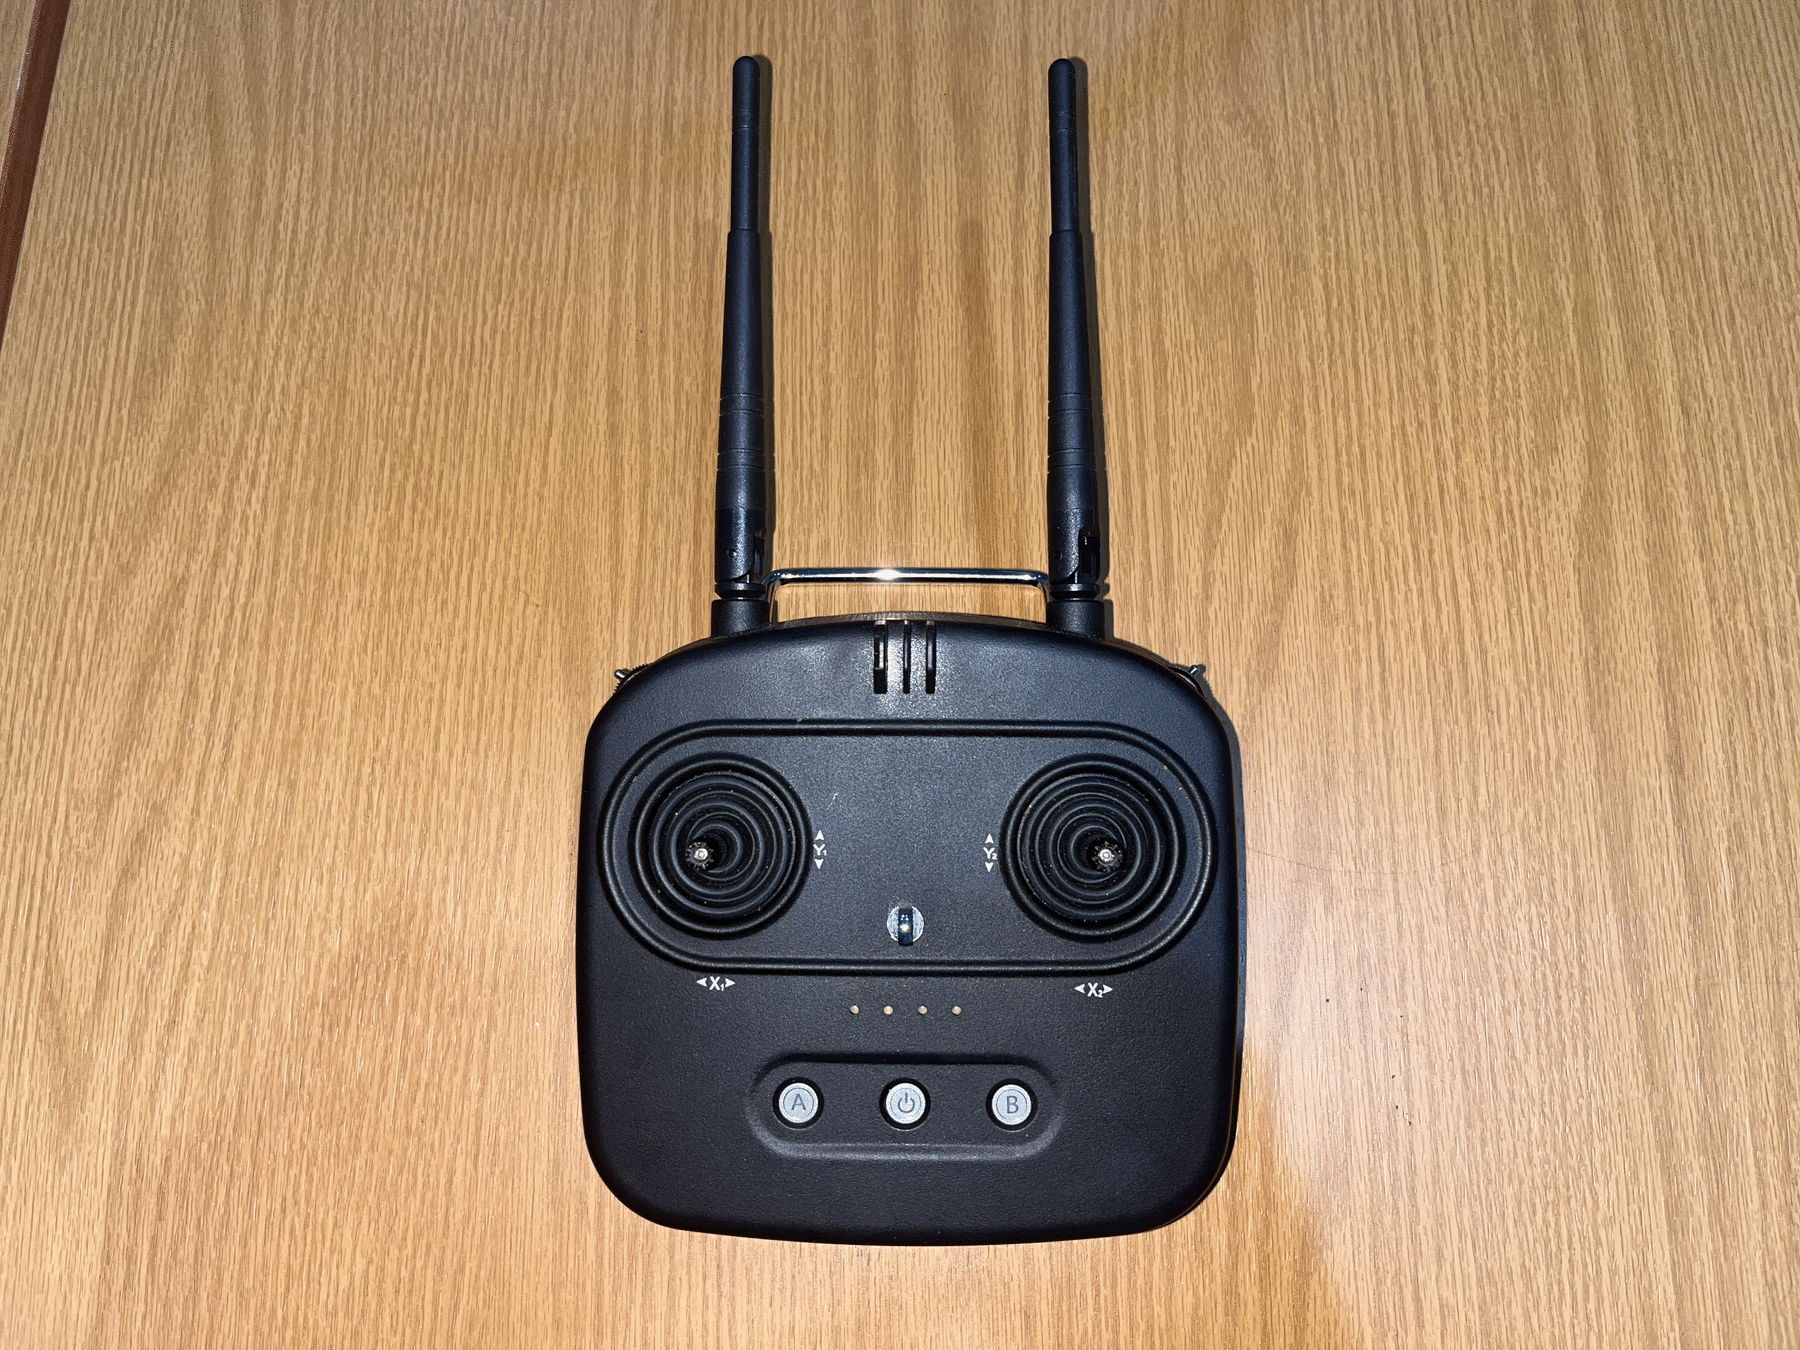
\includegraphics[width=0.6\linewidth]{bab3/rc_t10}
	\caption{Remote Controller T10 yang digunakan untuk transmisi kendali dan RC Override}
	\label{fig:rc_t10}
\end{figure}

Gambar \ref{fig:rc_t10} menunjukkan bentuk fisik unit pemancar radio kendali yang digunakan untuk mengoperasikan drone secara manual dan memicu mekanisme keselamatan. Berdasarkan implementasi tersebut, perangkat ini memegang peranan vital sebagai jembatan kendali darurat antara operator di darat dan unit autopilot PX4. Dapat diamati bahwa integrasi transmitter ini menyediakan saluran override fisik yang kebal terhadap kegagalan perangkat lunak di companion computer. Dengan demikian, keberadaan kendali radio ini menjadi lapisan pertahanan pertama dalam meminimalkan risiko kecelakaan selama misi otonom berlangsung.

\subsection{Perancangan Sistem Deteksi Manusia}
Perancangan sistem deteksi manusia dilakukan untuk menghasilkan kemampuan identifikasi korban secara otomatis menggunakan data visual dari kamera drone. Sistem deteksi manusia dirancang sebagai pipeline pemrosesan citra yang bekerja secara kontinu selama mode otonom aktif. Hasil deteksi kemudian digunakan sebagai dasar pengambilan keputusan navigasi drone selama proses pencarian berlangsung. Tahapan utama pada sistem deteksi manusia meliputi proses akuisisi citra, preprocessing, deteksi manusia, validasi target, dan distribusi informasi deteksi menuju sistem navigasi otonom dan sistem monitoring.

\begin{figure}[H]
	\centering
	
\includegraphics[width=\linewidth]{bab3/flow3-4.pdf}
	\caption{Blok Diagram Alur Deteksi Orang}
	\label{fig:blokdiagram4}
\end{figure}

Gambar \ref{fig:blokdiagram4} menunjukkan diagram alur pemrosesan data visual dari sensor webcam hingga menjadi informasi deteksi korban. Berdasarkan implementasi tersebut, aliran data citra mentah diolah melalui beberapa tahap fungsional untuk menghasilkan estimasi spasial target. Dapat diamati bahwa pembagian tahapan ini memastikan setiap proses mulai dari akuisisi hingga validasi berjalan secara teratur dan berulang. Dengan demikian, alur pemrosesan deteksi ini mampu memasok koordinat target secara konsisten ke modul pengendali otonom.

\subsubsection{Akuisisi Citra}
Akuisisi citra dilakukan menggunakan kamera webcam yang dipasang pada drone. Kamera mengambil frame citra secara kontinu selama sistem berjalan untuk menyediakan data visual bagi sistem deteksi manusia. Frame yang diperoleh kemudian dikirimkan menuju modul pemrosesan citra untuk dianalisis lebih lanjut oleh model deteksi. Proses akuisisi citra dirancang agar mampu menyediakan aliran data visual secara stabil sehingga sistem tetap dapat melakukan deteksi secara real-time selama drone bergerak dan menjalankan misi pencarian korban.

\subsubsection{Preprocessing Citra}
Tahap preprocessing dilakukan untuk menyesuaikan karakteristik citra dengan kebutuhan model deteksi manusia. Pada tahap ini citra mengalami beberapa proses penyesuaian seperti perubahan ukuran citra, normalisasi nilai piksel, dan penyesuaian format input model. Tahap preprocessing bertujuan untuk meningkatkan kestabilan proses inferensi dan menjaga kompatibilitas data terhadap model deteksi yang digunakan sehingga proses deteksi dapat berjalan secara optimal pada companion computer.

\subsubsection{Deteksi Manusia}
Tahap deteksi manusia dilakukan menggunakan model YOLOv8 berformat ONNX (Open Neural Network Exchange) dengan resolusi input sebesar 320x320 piksel. Model ini bertugas mengidentifikasi keberadaan manusia pada citra hasil preprocessing. Dari proses inferensi tersebut, model menghasilkan beberapa informasi utama berupa posisi bounding box, label kelas objek, dan nilai confidence untuk setiap objek yang terdeteksi. Hasil deteksi ini kemudian digunakan sebagai dasar penentuan target yang akan didekati oleh drone selama misi pencarian berlangsung. Dengan spesifikasi model tersebut, sistem mampu melakukan identifikasi manusia secara otomatis dan lebih efisien berdasarkan data visual yang diperoleh dari kamera webcam.

\subsubsection{Validasi dan Target Lock}
Untuk meningkatkan kestabilan navigasi drone, sistem menerapkan mekanisme validasi target dan target lock. Pada tahap ini sistem melakukan evaluasi terhadap objek hasil deteksi berdasarkan ukuran bounding box, nilai confidence, posisi objek terhadap pusat frame, dan konsistensi deteksi antar frame. Mekanisme target lock digunakan untuk mencegah perpindahan target secara tiba-tiba ketika terdapat lebih dari satu manusia pada area pengamatan kamera. Dengan pendekatan ini drone dapat mempertahankan fokus terhadap target yang sedang diamati sehingga pergerakan sistem menjadi lebih stabil selama proses pendekatan berlangsung.

\subsubsection{Distribusi Informasi Deteksi}
Setelah target berhasil diproses, hasil deteksi didistribusikan menuju sistem navigasi otonom dan sistem monitoring. Informasi deteksi digunakan oleh sistem otonom untuk menentukan perilaku navigasi drone, sedangkan pada sisi monitoring data digunakan untuk menampilkan hasil deteksi kepada operator secara real-time. Distribusi informasi ini memungkinkan sistem kontrol dan sistem monitoring berjalan secara bersamaan tanpa saling mengganggu proses utama drone selama operasi berlangsung.

\subsection{Perancangan Mesin Pengambil Keputusan}
Mesin pengambil keputusan merupakan bagian utama sistem otonom yang bertugas menentukan tindakan drone berdasarkan kondisi sistem dan hasil deteksi manusia. Pada tahap ini sistem mengintegrasikan data telemetri penerbangan dan informasi deteksi visual untuk menentukan aksi navigasi yang sesuai selama misi berlangsung. Pendekatan ini memungkinkan drone merespons perubahan kondisi lingkungan secara otomatis dan real-time sehingga perilaku sistem dapat tetap stabil selama operasi pencarian berlangsung.

\begin{figure}[H]
	\centering
	
\includegraphics[width=\linewidth]{bab3/flow3-5.pdf}
	\caption{Blok Diagram Alur Mesin Pengambil Keputusan}
	\label{fig:blokdiagram5}
\end{figure}

Gambar \ref{fig:blokdiagram5} menunjukkan arsitektur mesin pengambil keputusan otonom yang bekerja berdasarkan evaluasi kondisi sistem dan kejadian dinamis. Berdasarkan implementasi tersebut, drone dapat menentukan tindakan navigasi yang sesuai dengan prioritas misi dan status keselamatan. Dapat diamati bahwa pembagian logika ini menghasilkan transisi keputusan yang andal saat menangani kejadian tak terduga di lapangan. Dengan demikian, mesin pengambil keputusan ini menjamin kelancaran misi otonom dengan tetap mengutamakan aspek keselamatan terbang.

\subsubsection{Monitoring Kondisi Sistem}
Tahap monitoring kondisi sistem dilakukan secara kontinu selama mode otonom aktif. Sistem memantau beberapa parameter penting seperti status baterai, posisi drone, ketinggian penerbangan, kualitas GPS, dan mode penerbangan. Informasi tersebut digunakan untuk memastikan drone tetap berada pada kondisi operasional yang aman selama misi berlangsung. Selain itu, data telemetri yang diperoleh juga digunakan sebagai dasar evaluasi kondisi sistem sebelum drone menentukan tindakan navigasi berikutnya.

\subsubsection{Evaluasi Event}
Pada tahap evaluasi event, sistem melakukan identifikasi dan prioritas terhadap berbagai kondisi yang terjadi selama penerbangan. Sistem mengevaluasi keberadaan target manusia, kondisi baterai, kehilangan koneksi, serta perubahan status penerbangan yang dapat memengaruhi perilaku drone. Berdasarkan tingkat prioritasnya, sistem menentukan event mana yang harus diproses terlebih dahulu agar perilaku drone tetap stabil dan aman selama mode otonom aktif.

\subsubsection{Pemilihan Tindakan Otonom}
Setelah proses evaluasi selesai dilakukan, sistem menentukan tindakan navigasi yang akan dijalankan drone. Tindakan yang dapat dipilih meliputi rotasi pencarian, pendekatan target, dokumentasi korban, pergeseran posisi otonom, maupun prosedur keselamatan (\textit{safety procedure}) seperti Return to Launch (RTL). Pemilihan tindakan dilakukan secara otomatis berdasarkan kondisi sistem dan state aktif pada state machine sehingga drone mampu menyesuaikan perilaku secara dinamis selama operasi berlangsung.

\subsubsection{Siklus Pergeseran Posisi dan Kelanjutan Pencarian}
Tahap pergeseran posisi otonom (\texttt{DISPLACING}) secara lateral dilakukan setelah drone menyelesaikan proses dokumentasi target (\texttt{DOCUMENT}). Langkah ini bertujuan untuk melanjutkan misi pencarian korban secara persisten dengan memperluas cakupan area pengamatan. Setelah perpindahan lateral selesai atau jika drone kehilangan target yang sedang diamati, sistem akan kembali memasuki \textit{state} \texttt{SCAN} untuk memulai siklus pencarian baru. Logika otonom ini dirancang agar misi tetap berlanjut dan tidak melakukan pemulangan (\texttt{RETURN\_HOME}) dalam kondisi normal, karena skenario pulang akibat baterai kritis ditangani terpisah oleh fitur RTL bawaan PX4.

\section{Perencanaan dan Desain Sistem}
Tahap perencanaan dan desain sistem merupakan tahap lanjutan setelah perancangan perilaku sistem kontrol drone. Pada tahap ini, perilaku sistem yang telah dirumuskan sebelumnya diterjemahkan ke dalam bentuk rancangan teknis yang mencakup perangkat keras, perangkat lunak, dan arsitektur sistem secara keseluruhan. Tujuan utama dari tahap ini adalah memastikan bahwa sistem yang dirancang dapat direalisasikan secara teknis serta mendukung seluruh fungsi yang dibutuhkan selama operasi drone otonom.

\begin{figure}[H]
	\centering
	\includegraphics[width=0.8\linewidth]{bab3/flow3-6.pdf}
	\caption{Blok Diagram Alur Perencanaan dan Desain Sistem}
	\label{fig:blokdiagram6}
\end{figure}

Gambar \ref{fig:blokdiagram6} menunjukkan alur integratif dari perancangan arsitektur fisik, perangkat lunak, dan interkoneksi sistem secara keseluruhan. Berdasarkan implementasi tersebut, pembagian tugas rekayasa dapat direncanakan secara paralel untuk mempercepat perakitan dan pemrograman drone. Dapat diamati bahwa integrasi seluruh komponen pendukung dikelompokkan ke dalam tiga pilar desain utama guna menyederhanakan pelacakan kegagalan. Dengan demikian, rancangan terpadu ini menjadi dasar teknis dalam memproduksi purwarupa fisik drone otonom.

\subsection{Desain Hardware}
Tahap desain hardware berfokus pada perancangan komponen fisik yang mendukung operasional sistem drone. Sebelum merancang struktur mekanik dan kelistrikan pendukung, ditentukan terlebih dahulu dua perangkat keras utama yang menjadi pusat komputasi dan akuisisi data otonom.

Komponen pertama adalah Raspberry Pi 5 yang berfungsi sebagai \textit{companion computer}. Perangkat ini dipilih karena memiliki kapabilitas pemrosesan yang mumpuni untuk menjalankan seluruh arsitektur \textit{multi-thread}, mengeksekusi model deteksi manusia secara \textit{real-time}, dan melayani transmisi data ke \textit{frontend}. Komponen kedua adalah sensor visual berupa \textit{Webcam} Logitech C922. Kamera ini diplih karena kemampuannya menangkap aliran video beresolusi tinggi dengan tingkat latensi rendah, yang merupakan syarat mutlak agar akurasi kotak pembatas (\textit{bounding box}) dari algoritma model deteksi manusia tetap sinkron dengan posisi fisik drone.

\begin{figure}[H]
	\centering
	\begin{subfigure}[b]{0.45\textwidth}
		\centering
		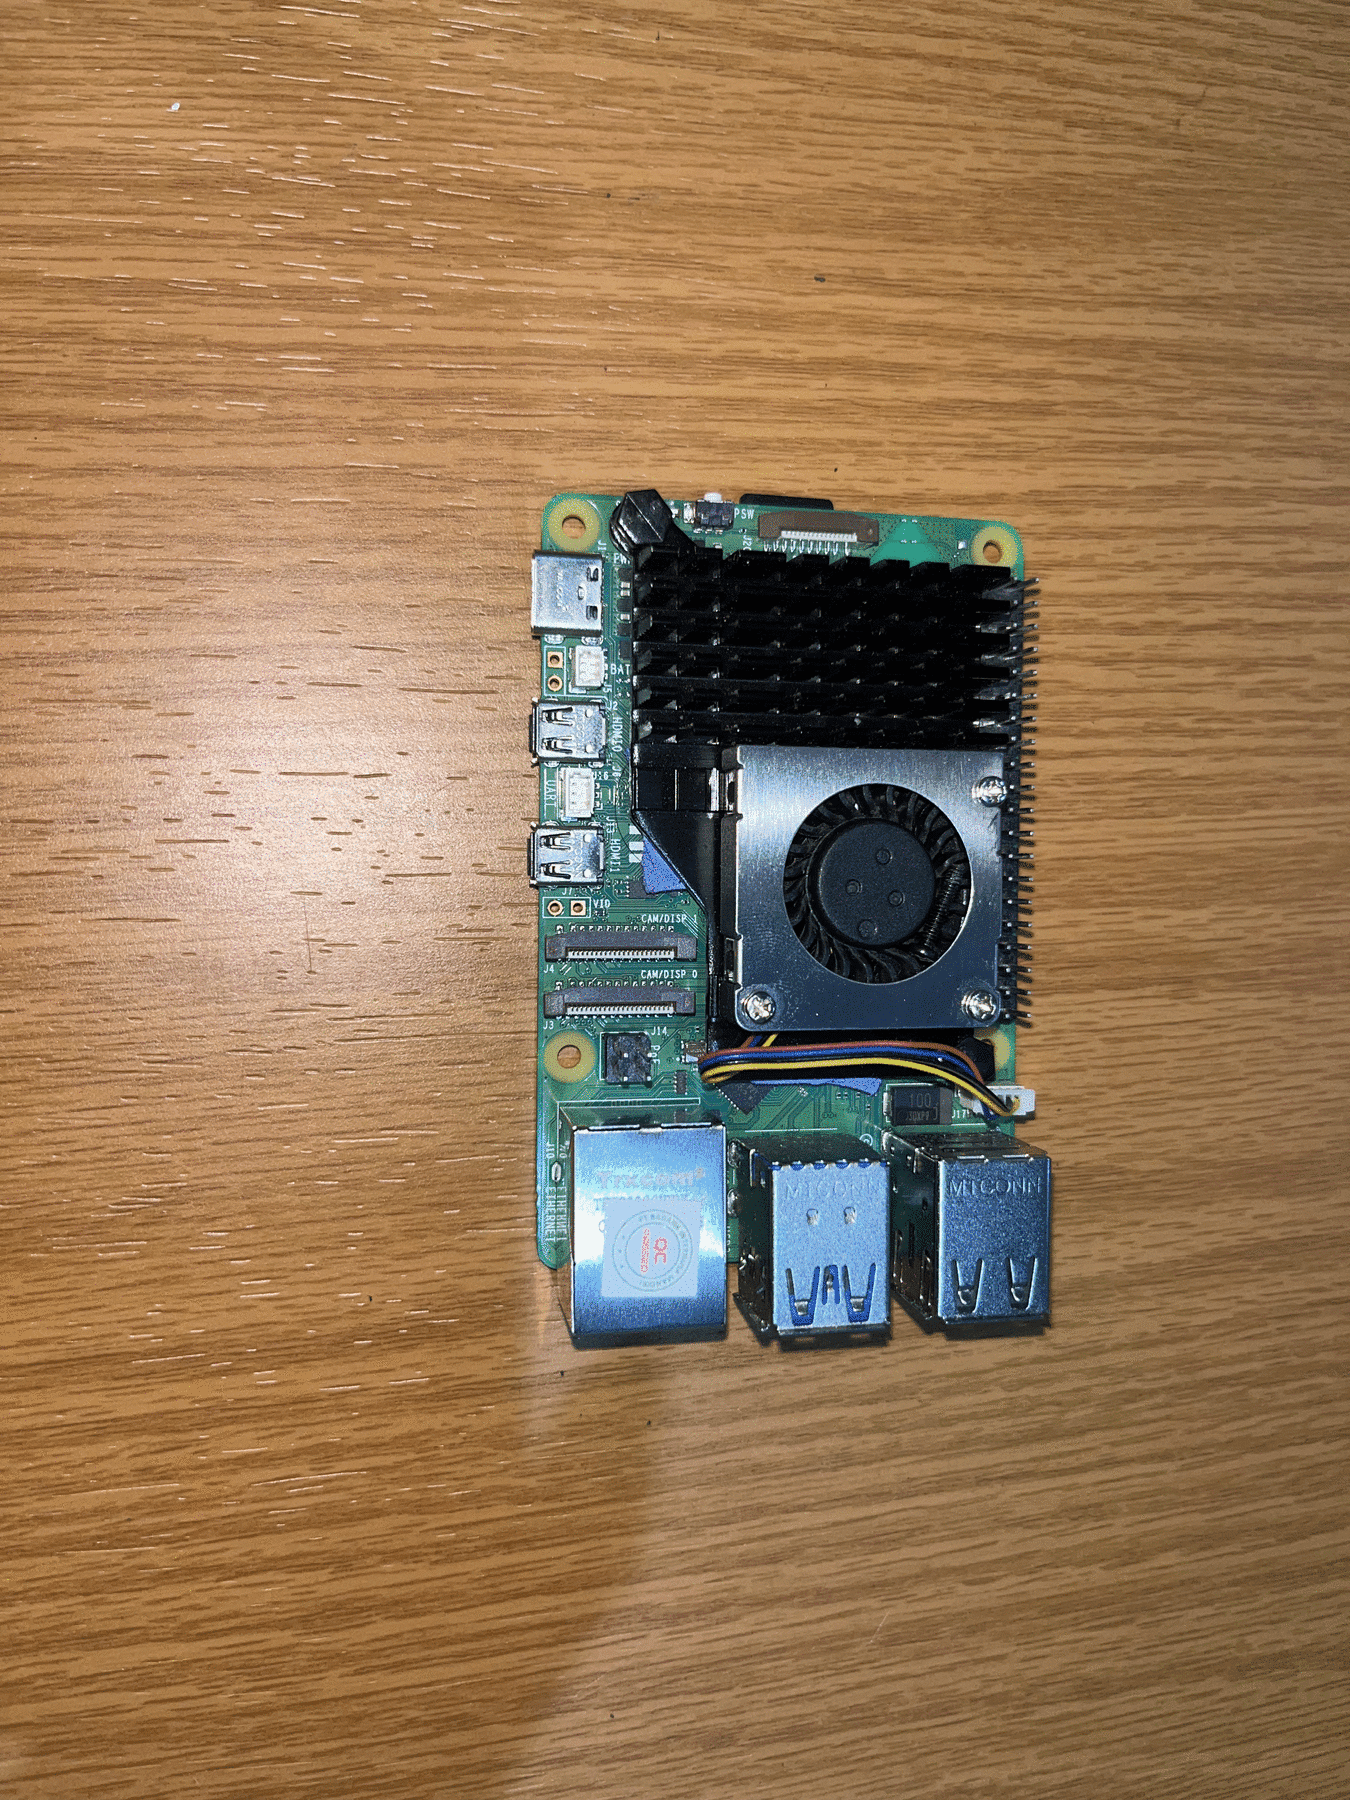
\includegraphics[width=\linewidth]{bab3/rpi5} 
		\caption{Unit komputasi utama Raspberry Pi 5}
		\label{fig:rpi5_raw}
	\end{subfigure}
	\hfill
	\begin{subfigure}[b]{0.45\textwidth}
		\centering
		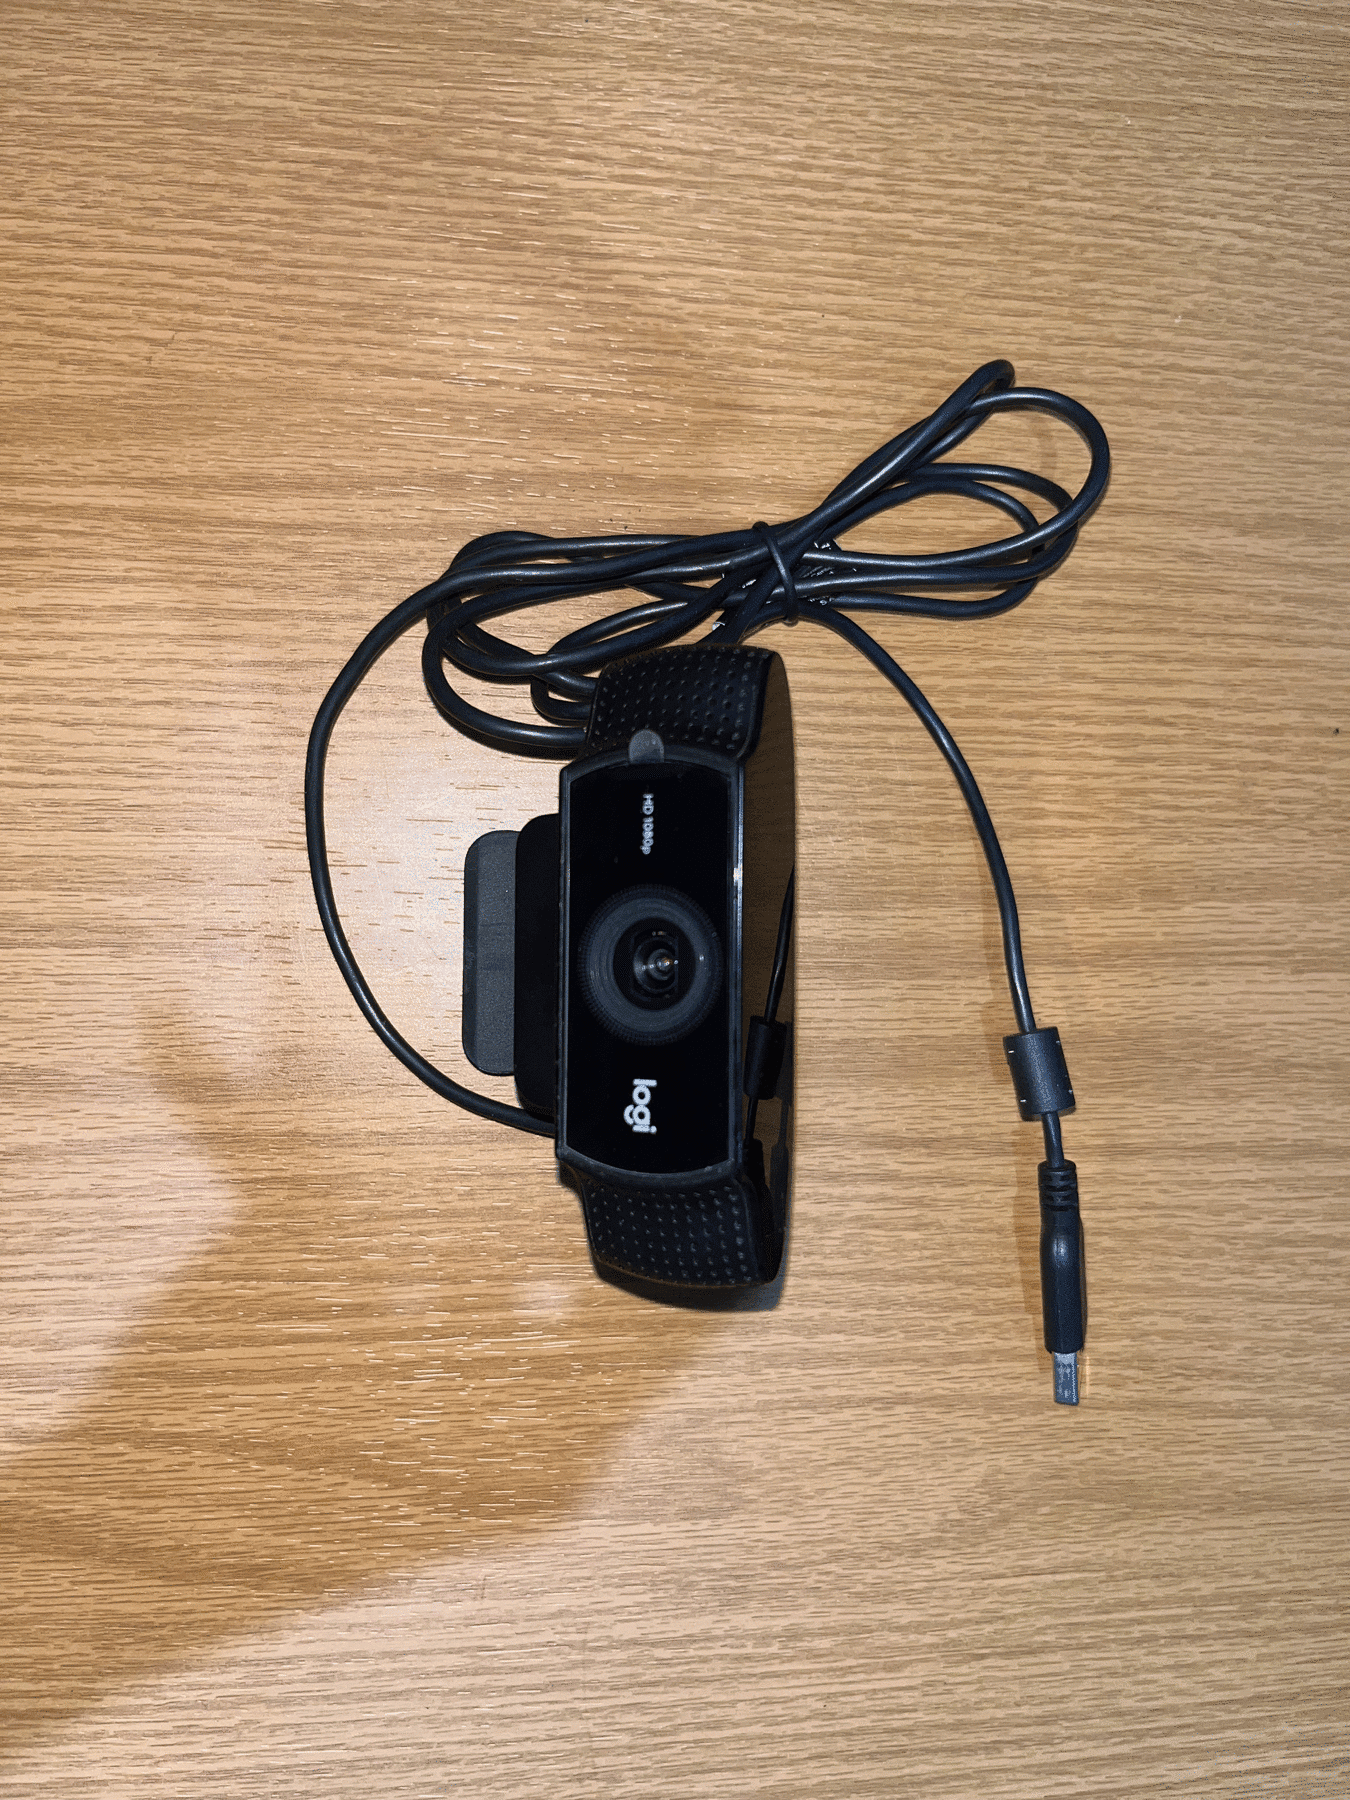
\includegraphics[width=\linewidth]{bab3/c922}
		\caption{Sensor visual utama Webcam Logitech C922}
		\label{fig:webcam_raw}
	\end{subfigure}
	\caption{Perangkat keras utama komputasi dan sensor visual}
	\label{fig:hardware_utama}
\end{figure}

Perancangan selanjutnya dilakukan terhadap sistem kelistrikan dan distribusi catu daya yang akan menyuplai perangkat-perangkat tersebut.

\subsubsection{Desain Elektrikal}
Desain elektrikal bertujuan untuk mengatur skema aliran daya ke seluruh komponen sistem drone, mencakup flight controller, sistem propulsi (motor dan ESC), serta companion computer (Raspberry Pi 5) beserta sensor visualnya (Webcam Logitech C922). Perancangan kelistrikan ini dibagi menjadi beberapa subsistem utama:
\begin{enumerate}
	\item Sistem Daya Utama Penerbangan (\textit{Main Power System})\\
	Sumber energi utama untuk keseluruhan sistem drone berasal dari baterai \textit{Lithium Polymer} (LiPo) 4S dengan kapasitas arus tinggi dan tegangan nominal 14,8 V. Distribusi daya utama diatur melalui mekanisme berikut:
	\begin{itemize}
		\item XT60 Y-Splitter: Baterai terhubung ke konektor XT60 \textit{Y-Splitter female to 2 male} yang berfungsi sebagai titik percabangan paralel primer. Jalur pertama diarahkan menuju sistem penggerak (\textit{Power Module \& PDB}), sementara jalur kedua didedikasikan untuk sistem komputasi pendukung melalui UBEC 5A.
		\item Power Module \& PDB: Pada jalur penerbangan, daya mengalir melalui \textit{Power Module} yang berfungsi sebagai sensor arus dan tegangan untuk dikirimkan ke Pixhawk sebagai data telemetri baterai. Output dari \textit{Power Module} diteruskan ke \textit{Power Distribution Board} (PDB) pada rangka Holybro S500 untuk didistribusikan secara paralel ke empat \textit{Electronic Speed Controller} (ESC).
		\item \textit{Regulasi Tegangan FCU}: \textit{Power Module} juga melakukan regulasi tegangan menjadi 5V DC yang terisolasi untuk menyuplai daya ke Pixhawk \textit{Flight Controller Unit} (FCU), memastikan sistem navigasi tetap aktif secara stabil meskipun terjadi fluktuasi arus pada motor \textit{brushless}.
	\end{itemize}
	
	\item Sistem Daya Pendukung Komputasi (\textit{Companion Computer Power})\\
	Suplai daya untuk komputasi otonom dan pemrosesan visual pada Raspberry Pi 5 dirancang melalui proses iterasi kelistrikan guna mendapatkan stabilitas operasional yang optimal.
	
	\begin{enumerate}
		\item Desain Kelistrikan Awal\\
		\begin{enumerate}
			\item Modul Mini UPS 18650: Dirancang untuk menyuplai daya awal melalui pin ekspansi GPIO. Modul ini memiliki spesifikasi tegangan input (\textit{input}) maksimal 5V, tegangan keluaran (\textit{output}) 5V, arus maksimal 3A, dan batas daya regangan sebesar 15W.
			\item Regulator Step-Down XL4015E1: Dirancang untuk menurunkan tegangan dari konfigurasi baterai 18650 2S. Spesifikasi modul ini memiliki rentang tegangan input 8V--36V, tegangan keluaran yang dapat diatur (\textit{adjustable}) antara 1.25V--32V, dengan efisiensi konversi sebesar 96\%, dan arus keluaran maksimal sebesar 5A.
			\item Regulator Step-Down XL4016E1: Dipilih sebagai opsi peningkatan kapasitas daya dengan spesifikasi rentang tegangan input 4V--40V, tegangan keluaran \textit{adjustable} 1.25V--36V, frekuensi \textit{switching} 180 kHz, dan arus keluaran maksimal mencapai 8A.
			\item Modul UBEC (\textit{Universal Battery Elimination Circuit}) 5A: Dirancang untuk skema kelistrikan revisi akhir. Memiliki spesifikasi input 5.5V--26V (2S--6S LiPo), keluaran stabil pada tegangan 5V, dan kemampuan hantaran arus kontinu sebesar 5A dengan perlindungan \textit{noise} elektromagnetik.
		\end{enumerate}
		
		Perancangan jalur distribusi daya juga mengalami perubahan dari yang awalnya direncanakan memanfaatkan pin ekspansi GPIO hingga dialihkan menuju port input USB-C bawaan Raspberry Pi 5 guna memanfaatkan sirkuit regulasi internal board.
		
		\item Desain Kelistrikan Akhir (Berbasis UBEC 5A)\\
		Untuk mengatasi kendala \textit{under-voltage}, desain kelistrikan akhir diimplementasikan menggunakan modul UBEC 5A tersebut yang disuplai langsung oleh baterai LiPo. Baterai LiPo memiliki tingkat pelepasan arus (\textit{C-Rating}) yang sangat tinggi sehingga memastikan Raspberry Pi 5 menerima tegangan 5V yang stabil tanpa \textit{drop}. Konfigurasi desain kelistrikan ini mendukung dua mode operasional:
		
		\begin{enumerate}
			\item Konfigurasi Baterai Tunggal (Paralel)\\
			Memanfaatkan satu baterai utama drone (LiPo 4S). Distribusi daya dicabangkan dari PDB menuju ESC/motor dan secara paralel dialirkan menuju modul UBEC 5A untuk Raspberry Pi 5. Keunggulan konfigurasi ini terletak pada efisiensi bobot (\textit{payload}).
			
			\item Konfigurasi Baterai Ganda (Terisolasi)\\
			Menggunakan dua baterai LiPo terpisah. Satu baterai didedikasikan untuk PDB dan sistem propulsi, sementara satu baterai sekunder dihubungkan khusus untuk menyuplai UBEC 5A ke Raspberry Pi 5. Konfigurasi ini menjamin isolasi daya penuh dari fluktuasi tegangan saat motor menarik arus maksimal, meskipun menambah beban angkut keseluruhan.
		\end{enumerate}
	\end{enumerate}
	
	\item Koneksi Data dan Komunikasi\\
	Antarmuka komunikasi antara Raspberry Pi 5 dan Pixhawk 6C dirancang untuk memastikan pengiriman pesan protokol MAVLink berjalan secara \textit{real-time} dan stabil. Berdasarkan pengujian operasional, transmisi data terbukti berjalan lancar tanpa kendala referensi tanah (\textit{ground reference}) atau interferensi \textit{ground loop}, baik saat sistem disuplai oleh konfigurasi baterai LiPo tunggal (menggunakan konektor XT60 \textit{Y-Splitter} ke PDB dan UBEC 5A) maupun konfigurasi baterai LiPo ganda. Sistem mendukung dua skenario antarmuka fisik yang fleksibel:
	\begin{enumerate}[]
		\item Koneksi Serial UART (Kabel JST)\\
		Menggunakan jalur komunikasi serial langsung ke \textit{port} TELEM3 pada Pixhawk. Jalur data ini ideal untuk integrasi \textit{library} MAVSDK Python dengan manajemen kabel yang ringkas. 
		
		Penggunaan jalur komunikasi ini mewajibkan adanya konfigurasi awal pada sistem operasi Raspberry Pi. Pengaturan dilakukan melalui antarmuka terminal dengan menjalankan perintah \texttt{sudo raspi-config}. Pada menu yang muncul, navigasi diarahkan ke Interface Options, kemudian pilih Serial Port. Sistem akan memberikan dua pertanyaan konfigurasi: pertama, pilih No untuk menonaktifkan login shell via serial; kedua, pilih Yes untuk mengaktifkan antarmuka serial port hardware. Menonaktifkan \textit{login shell} pada langkah pertama sangat krusial; apabila opsi ini dibiarkan aktif, sistem akan mengalokasikan jalur serial tersebut sebagai \textit{console login}, yang berakibat pada hilangnya akses remote ke Raspberry Pi melalui protokol SSH meski berada di dalam jaringan lokal yang sama.
		
		\begin{figure}[H]
			\centering
			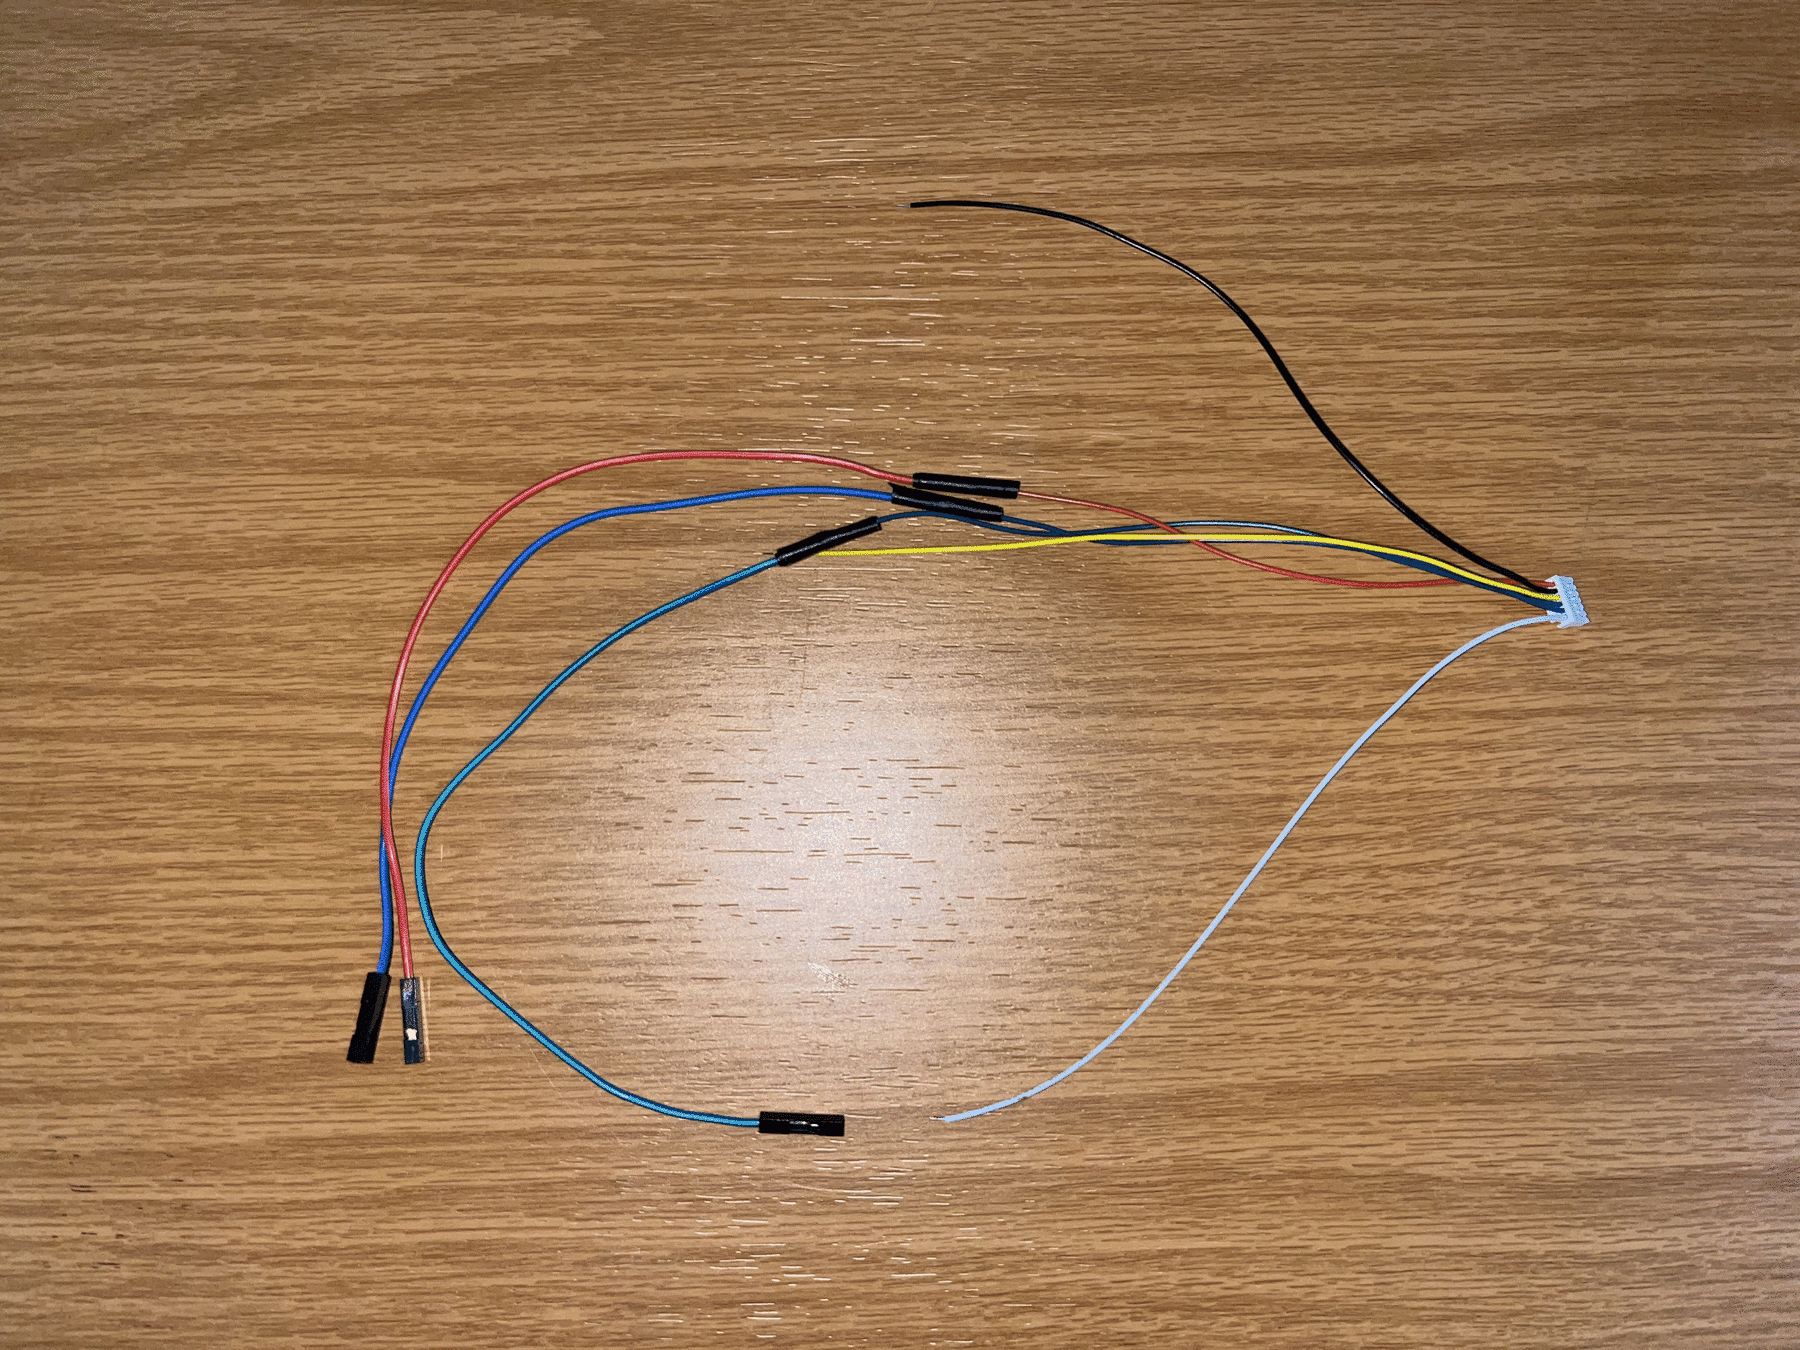
\includegraphics[width=0.5\textwidth]{bab3/kabel_konektor_serial} 
			\caption{Kabel konektor komunikasi serial (UART) untuk port TELEM3}
			\label{fig:kabel-serial}
		\end{figure}
		
		\item \textit{Direct USB Connection}\\
		Menggunakan koneksi kabel USB standar antara kedua perangkat. Metode ini sering diandalkan karena kemudahan \textit{plug-and-play} dan keandalan isolasi internal pada \textit{port} standar.
	\end{enumerate}
	Sebagai catatan tambahan, potensi masalah perbedaan potensial (\textit{ground loop}) secara teoritis hanya perlu diantisipasi apabila suplai daya Raspberry Pi diubah menggunakan modul UPS eksternal (dengan rentang daya 15-25 Watt yang bersumber dari dua buah baterai 18650 yang dirangkai seri). Namun, hal ini merupakan skenario periferal yang masih memerlukan pengujian lebih lanjut, sedangkan untuk standar operasional berbasis LiPo saat ini sistem dipastikan aman.
	Seluruh pengambilan citra tetap menggunakan antarmuka USB 3.0 khusus untuk \textit{webcam} Logitech C922 guna menjamin \textit{bandwidth} tinggi dan latensi rendah yang dibutuhkan untuk pemrosesan algoritma YOLOv8 secara \textit{real-time}.
	
	Untuk merealisasikan skema kelistrikan yang stabil-baik pada konfigurasi tunggal maupun terisolasi-diperlukan beberapa perangkat keras kelistrikan spesifik. Sumber energi utama mengandalkan baterai LiPo 4S yang dirawat tegangan selnya menggunakan \textit{Charger Balance} khusus agar siklus hidup baterai tetap optimal. Pada jalur distribusi daya, aliran arus dari baterai dicabangkan secara paralel menggunakan konektor XT60 \textit{Y-Splitter}. Cabang yang menuju sistem komputasi kemudian dihubungkan pada modul regulator UBEC 5A. Modul penurun tegangan (\textit{step-down}) ini berperan krusial dalam menyaring \textit{noise} listrik sekaligus memastikan Raspberry Pi 5 menerima suplai 5V konstan, terbebas dari fluktuasi saat motor propulsi menarik arus buang yang sangat besar.
	
	\begin{figure}[H]
		\centering
		\begin{subfigure}[b]{0.45\textwidth}
			\centering
			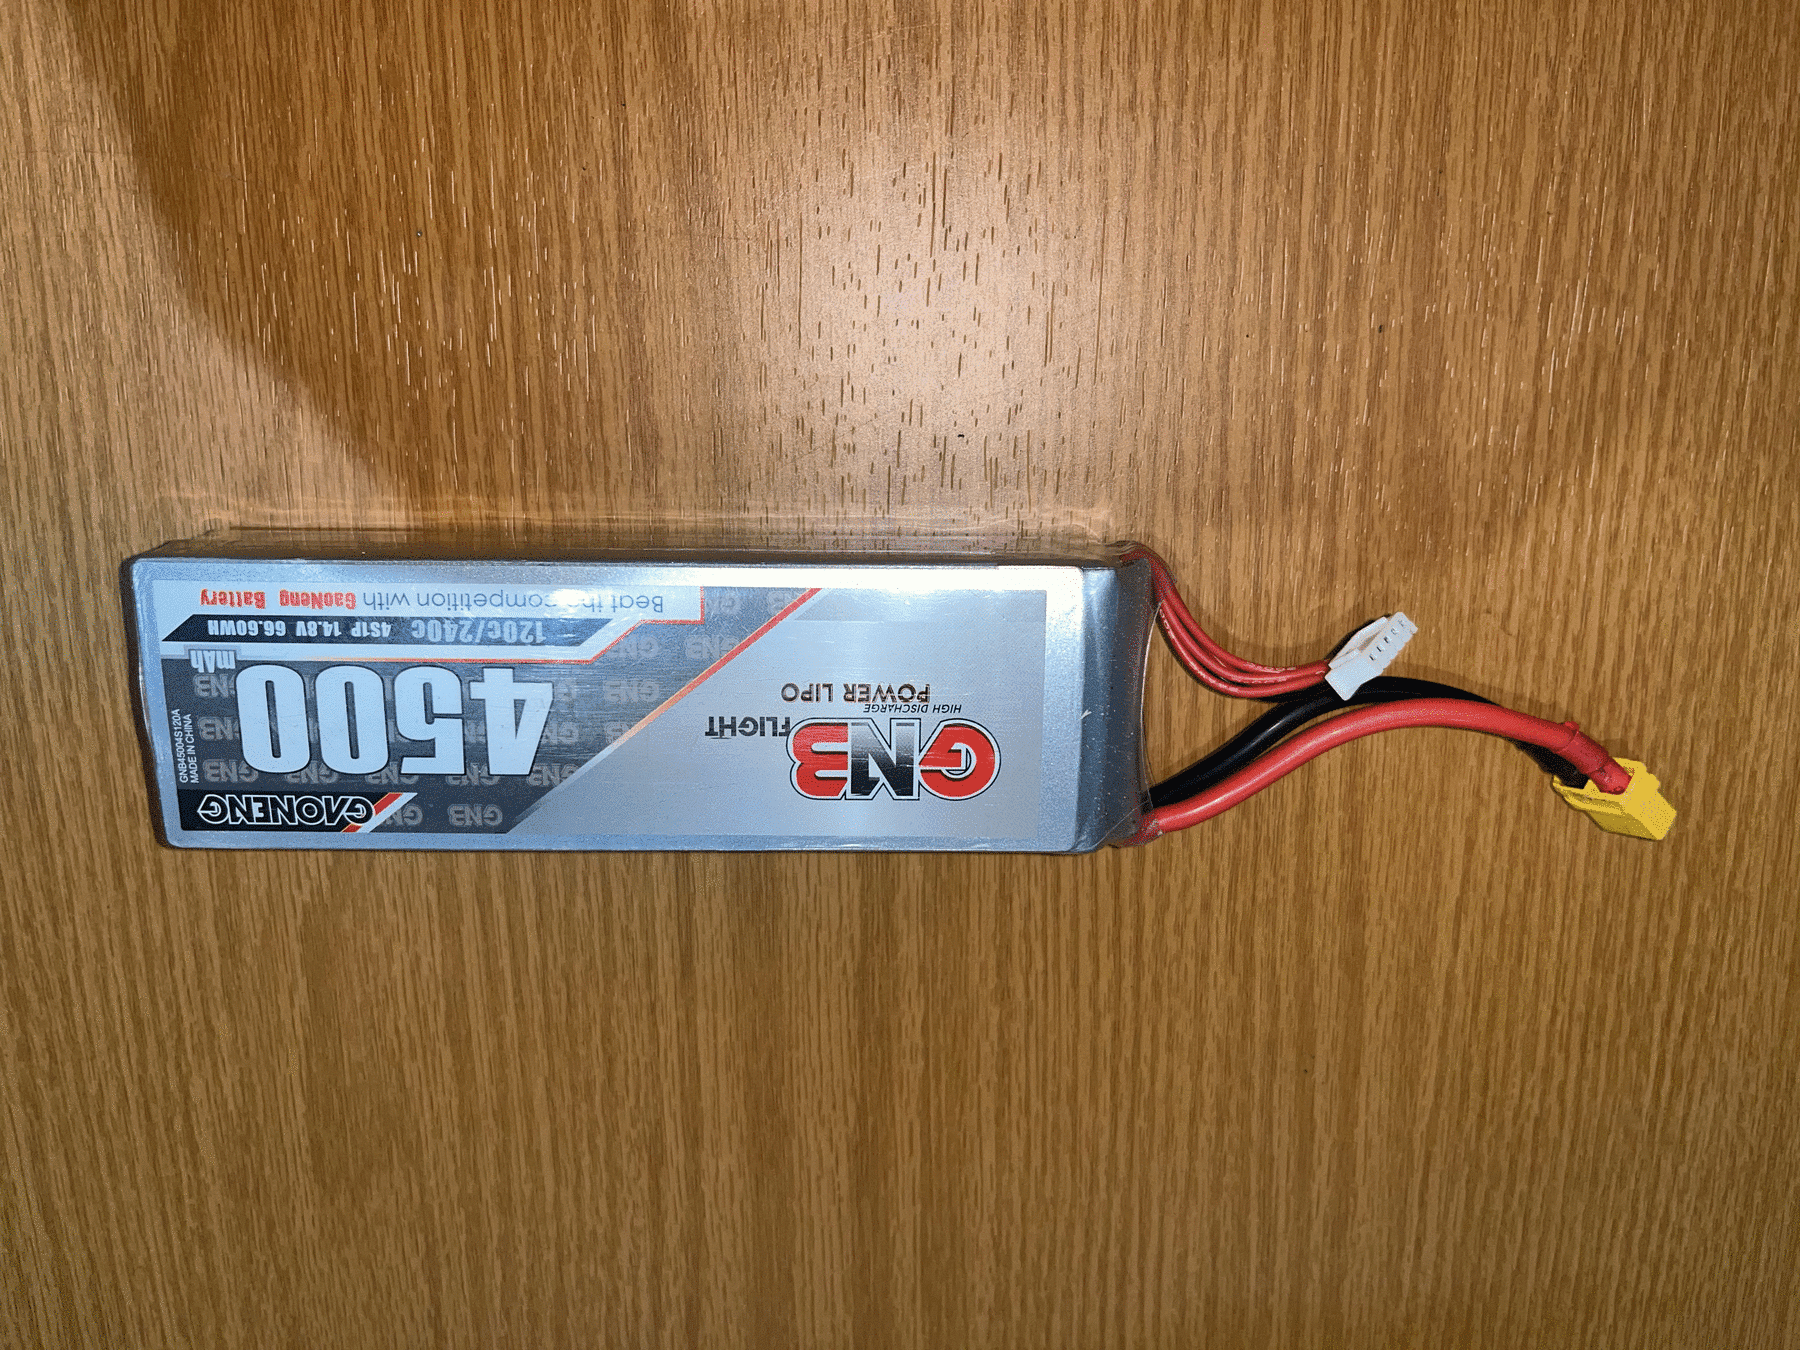
\includegraphics[width=\linewidth]{bab3/baterai_lipo}
			\caption{Baterai LiPo 4S utama drone}
			\label{fig:baterai_lipo_raw}
		\end{subfigure}
		\hfill
		\begin{subfigure}[b]{0.45\textwidth}
			\centering
			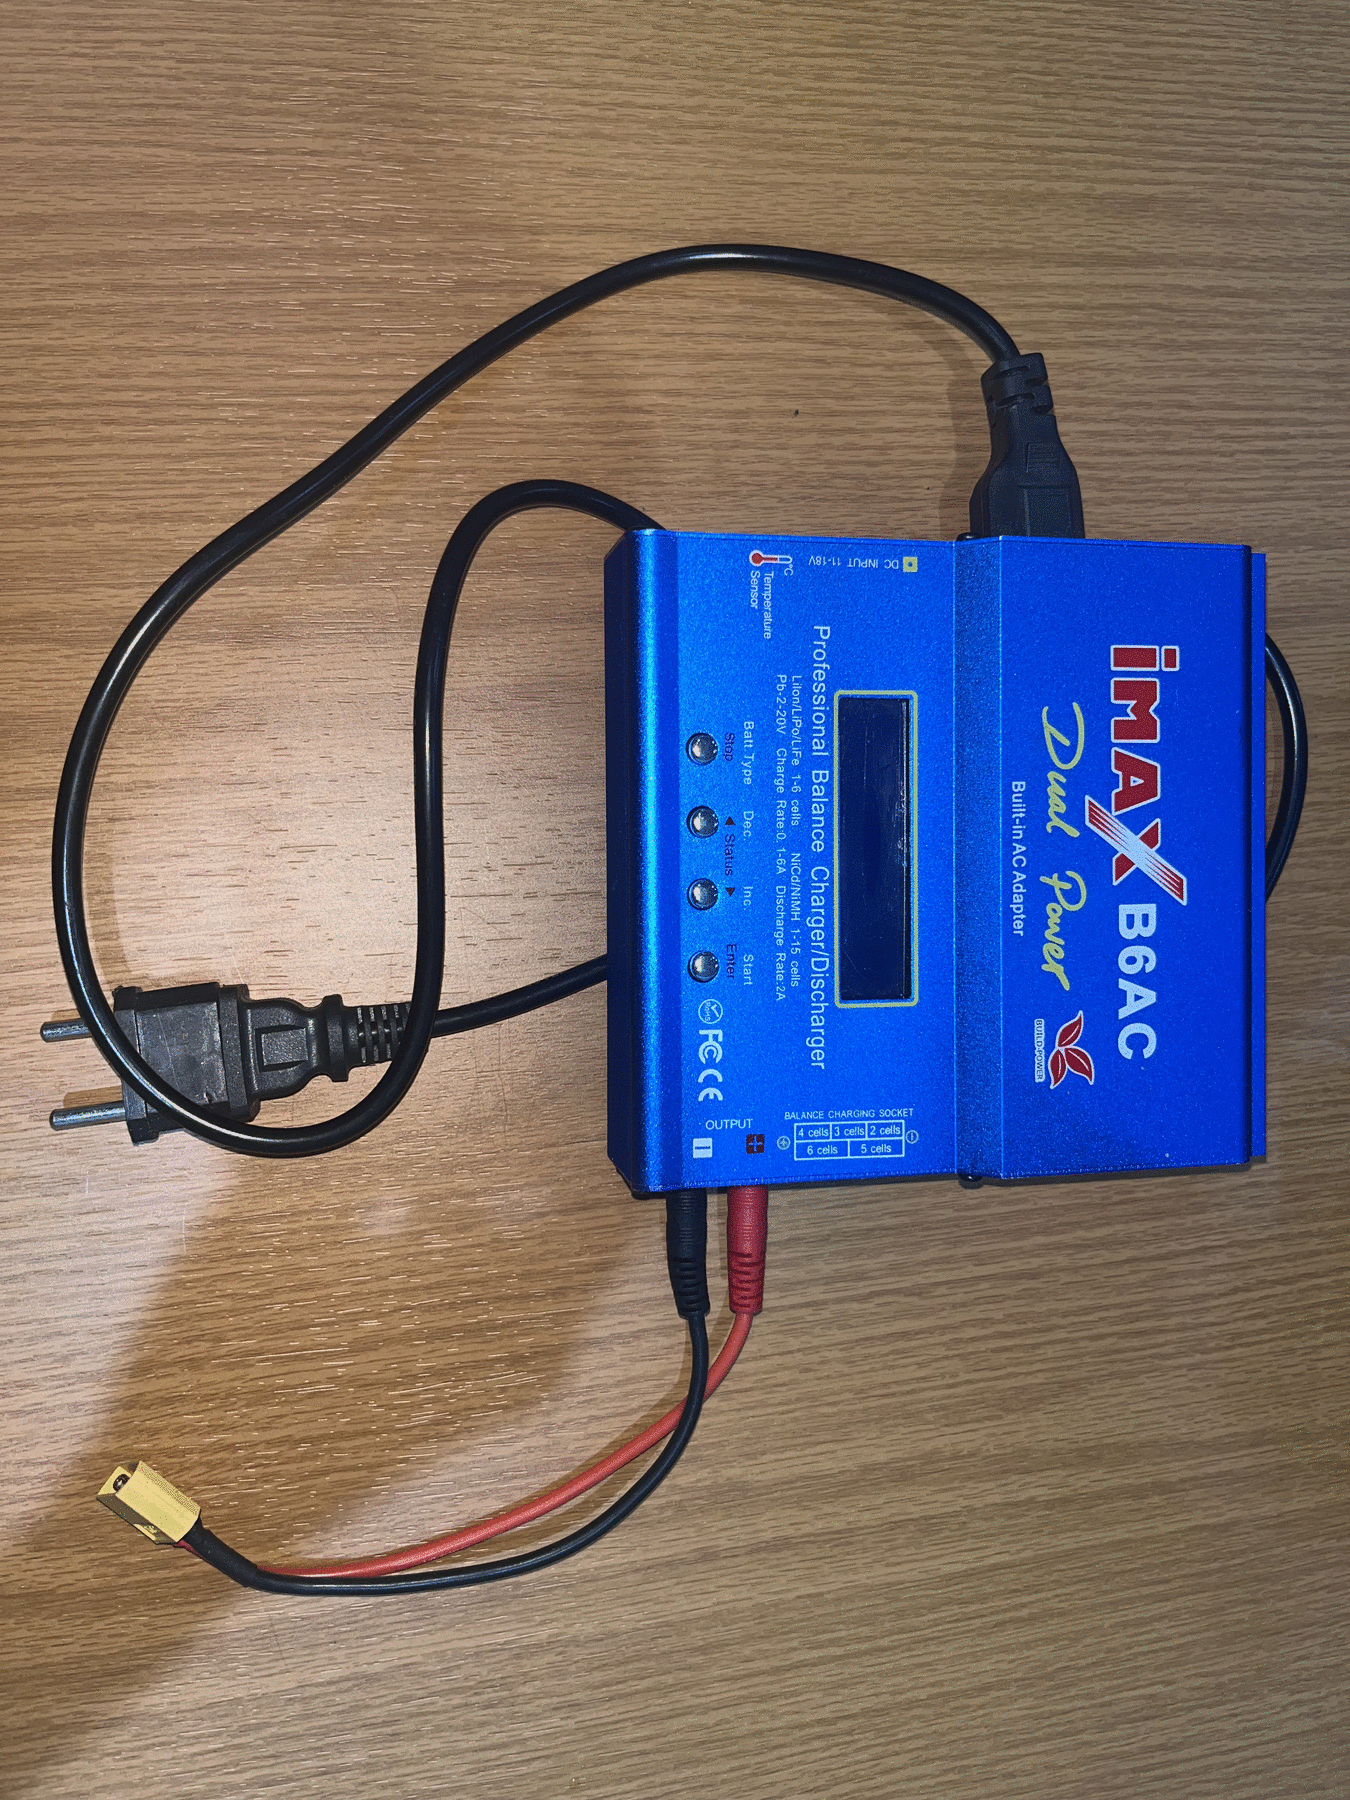
\includegraphics[width=\linewidth]{bab3/imax_charger_lipo}
			\caption{Charger Balance untuk perawatan baterai}
			\label{fig:charger_balance}
		\end{subfigure}
		
		\vspace{0.5cm} 
		
		\begin{subfigure}[b]{0.3\textwidth}
			\centering
			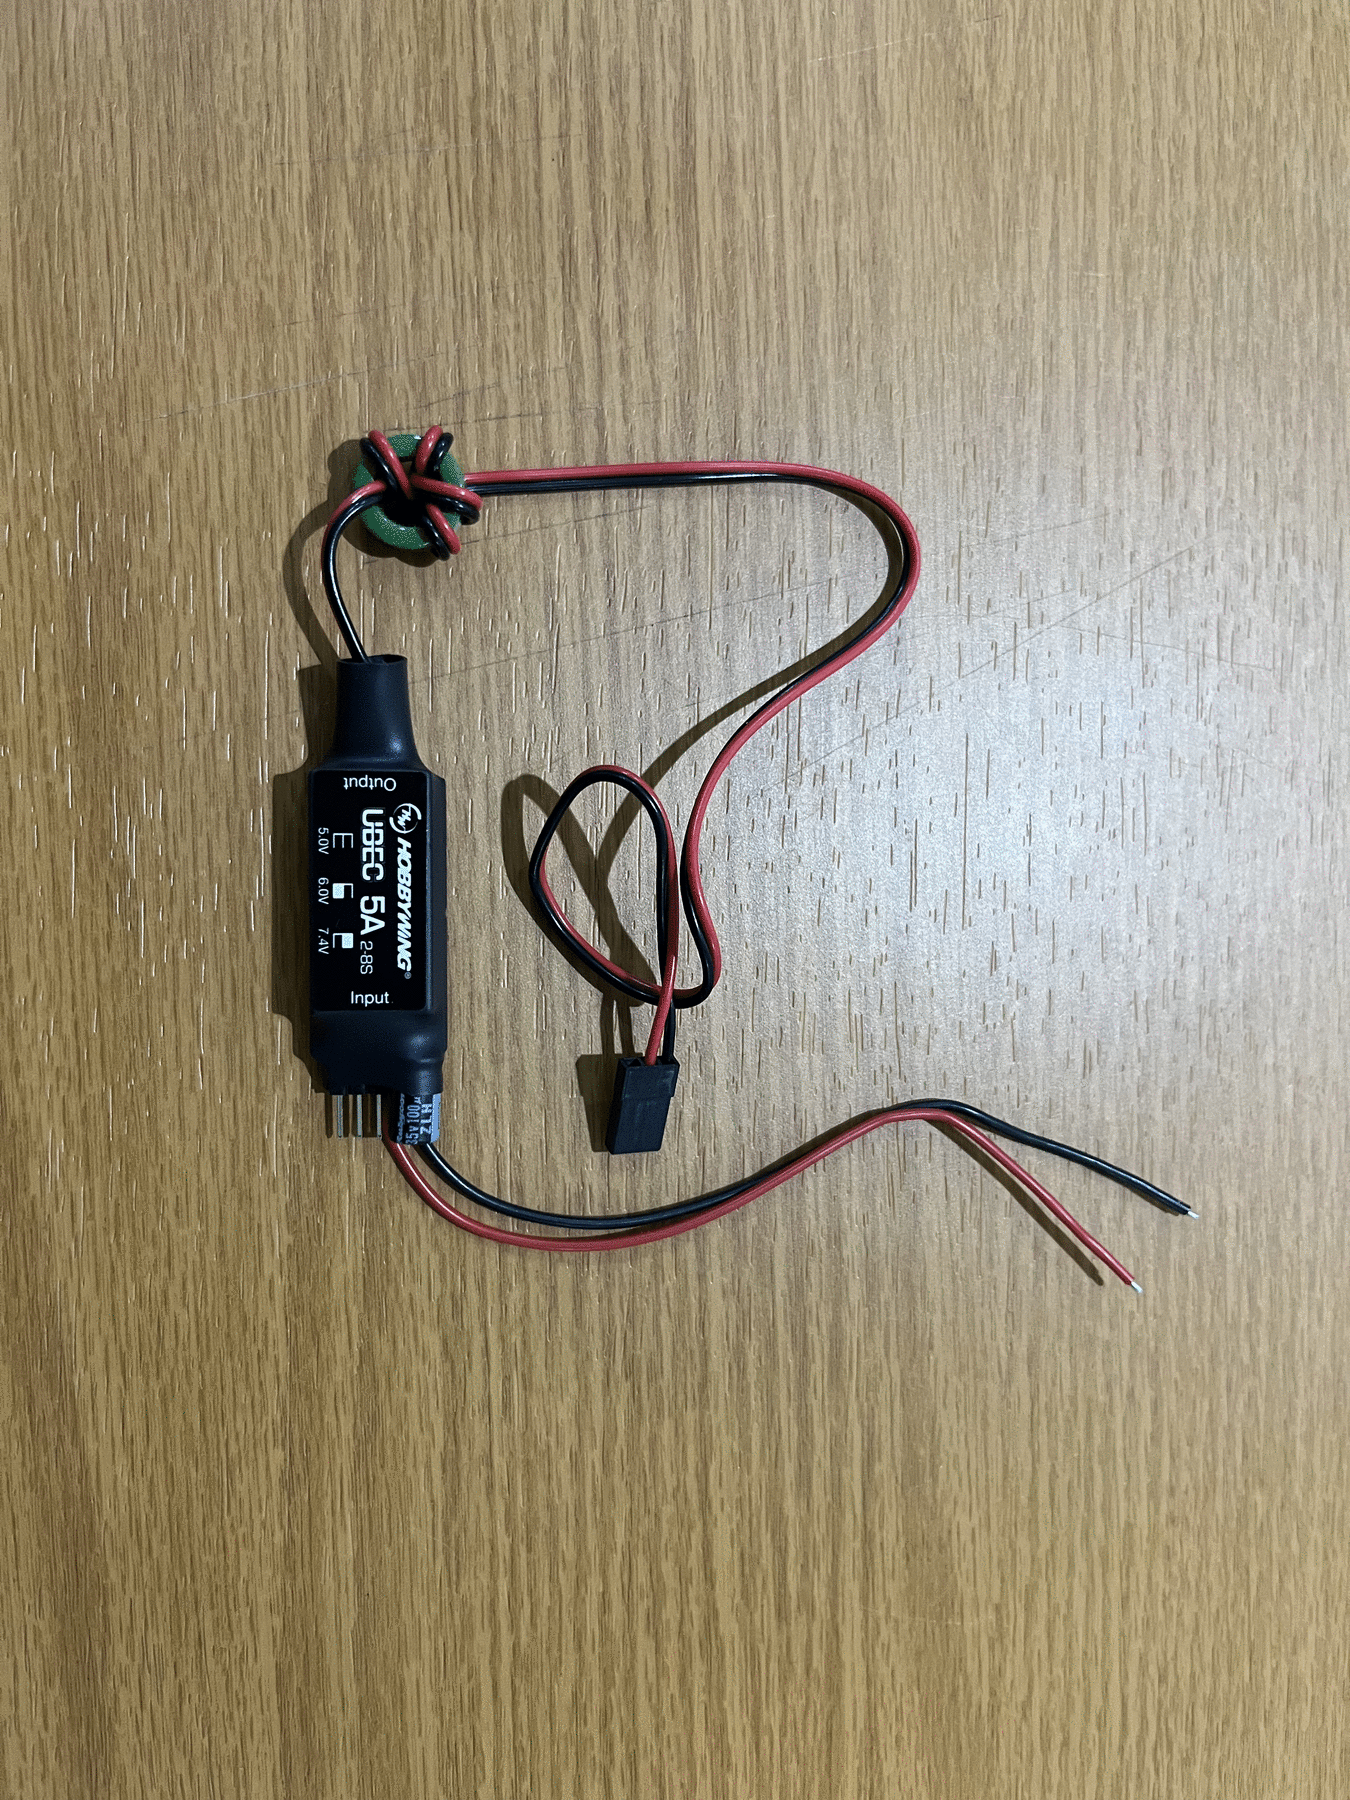
\includegraphics[width=\linewidth]{bab3/ubec}
			\caption{Modul Regulator Daya UBEC 5A}
			\label{fig:ubec_raw}
		\end{subfigure}
		\hfill
		\begin{subfigure}[b]{0.3\textwidth}
			\centering
			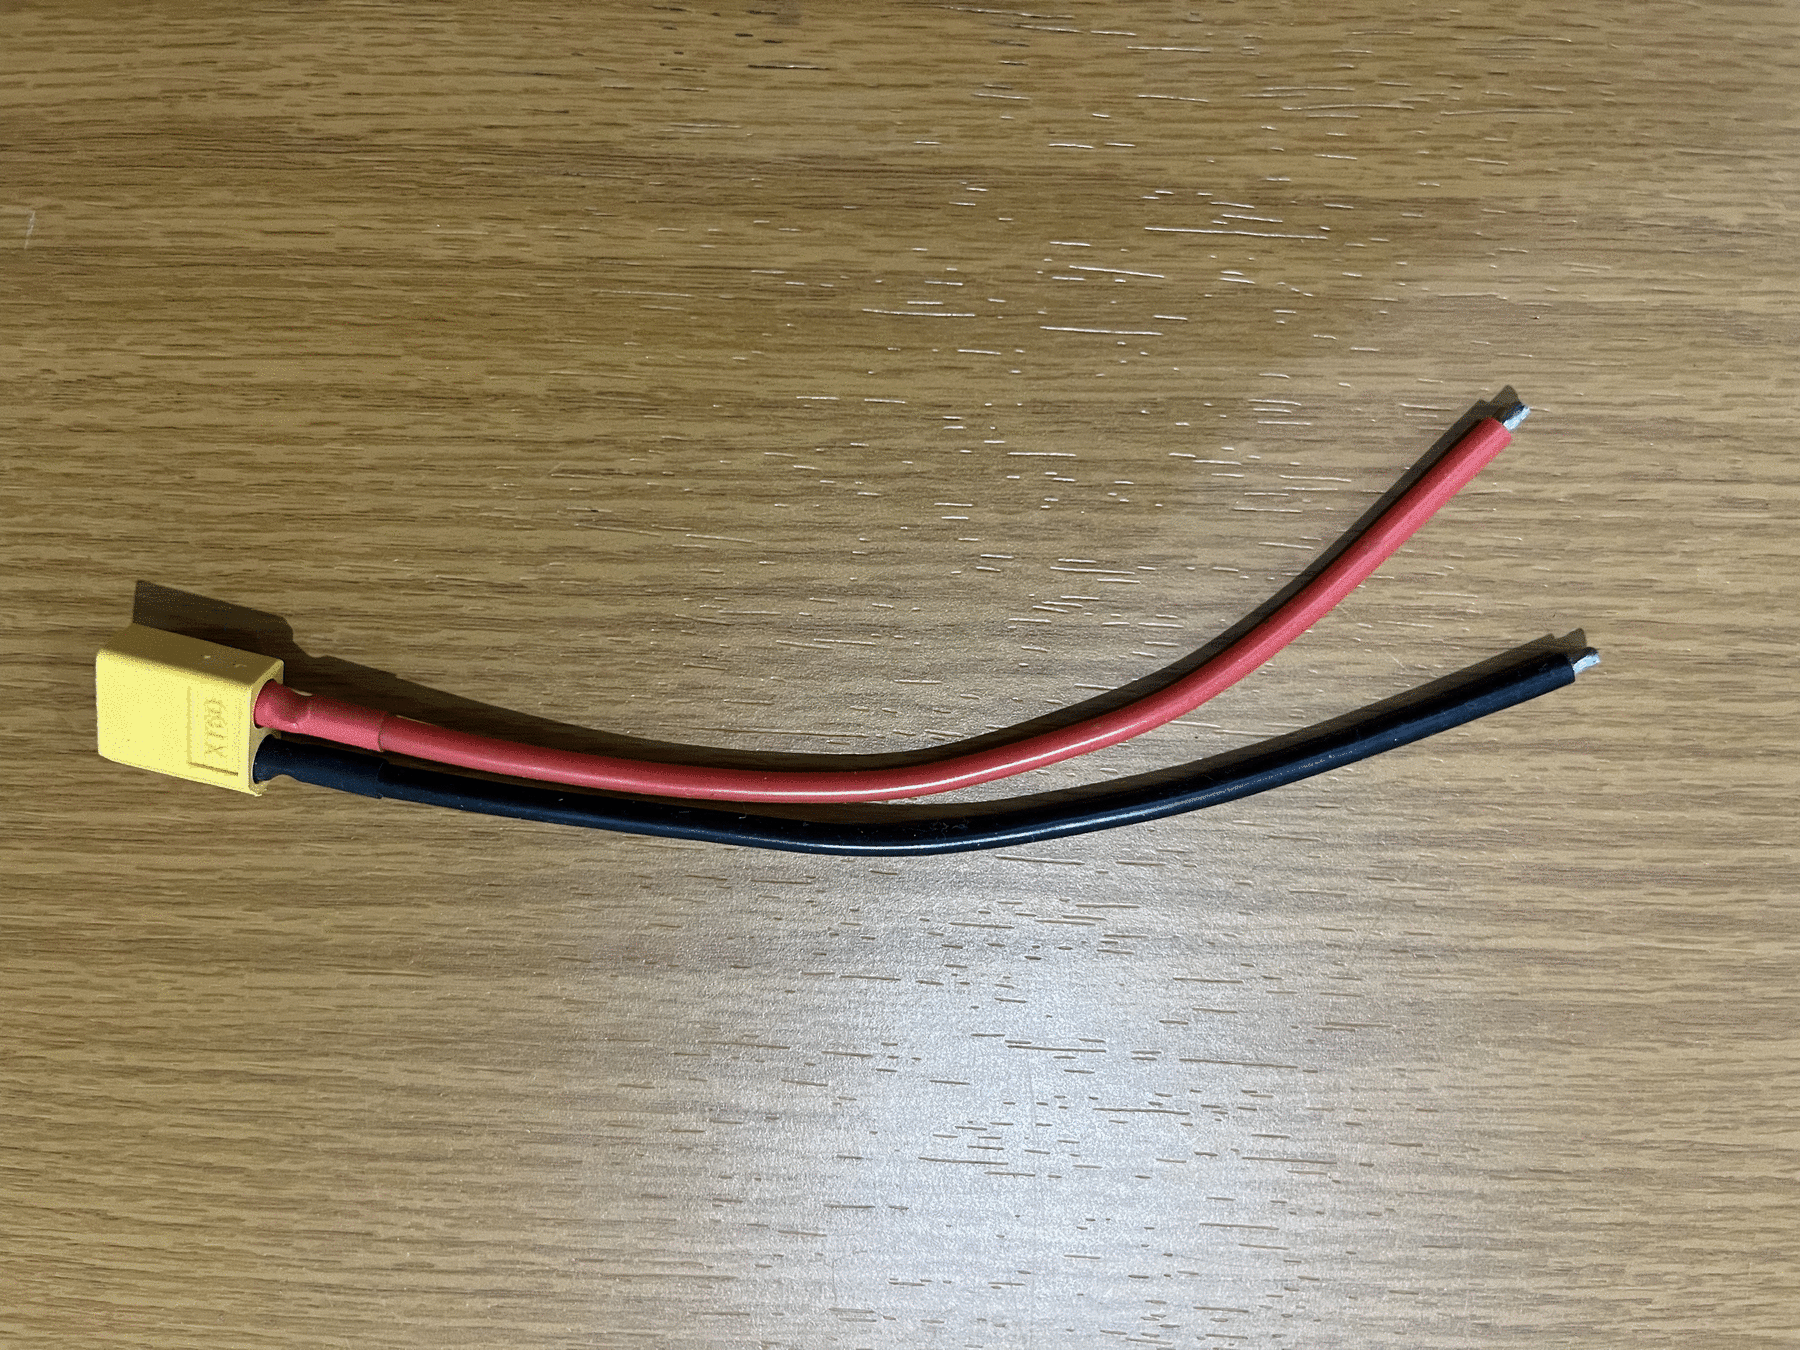
\includegraphics[width=\linewidth]{bab3/xt60_male}
			\caption{Konektor XT60 Male}
			\label{fig:xt60_male}
		\end{subfigure}
		\hfill
		\begin{subfigure}[b]{0.3\textwidth}
			\centering
			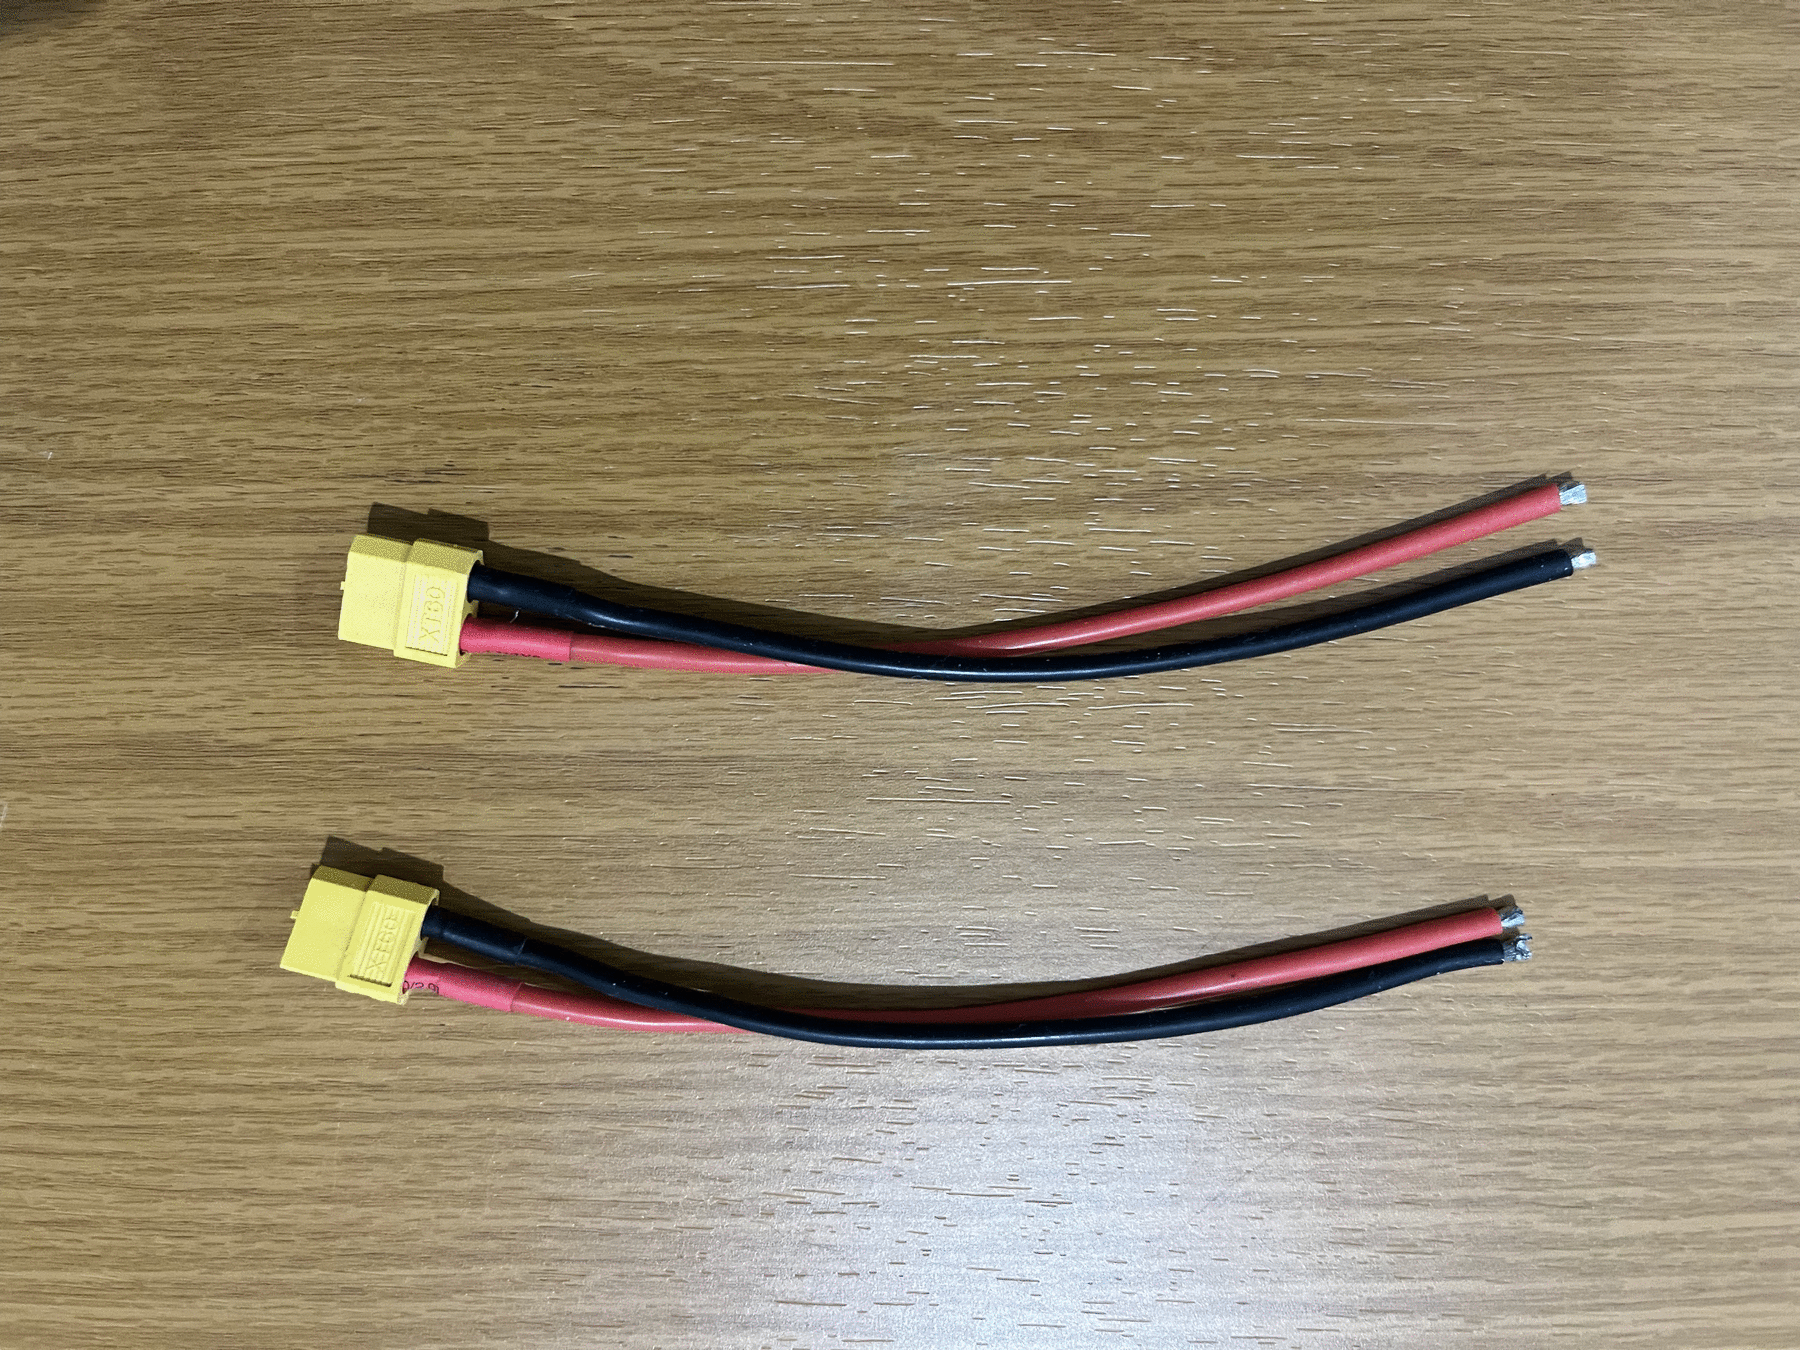
\includegraphics[width=\linewidth]{bab3/xt60_female}
			\caption{Konektor XT60 Female}
			\label{fig:xt60_female}
		\end{subfigure}
		\caption{Komponen perangkat keras pendukung sistem elektrikal}
		\label{fig:komponen_elektrikal}
	\end{figure}
	
	\item Skema Distribusi Daya
	\begin{figure}[H]
		\centering
		\includegraphics[width=0.7\linewidth]{bab3/flow3-7.pdf}
		\caption{Blok Diagram Konfigurasi Baterai Tunggal (Paralel)}
		\label{fig:blokdiagram7}
	\end{figure}
	
	\begin{figure}[H]
		\centering
		\includegraphics[width=0.7\linewidth]{bab3/flow3-8.pdf}
		\caption{Blok Diagram Konfigurasi Baterai Ganda (Terisolasi)}
		\label{fig:blokdiagram8}
	\end{figure}
	
\end{enumerate}

Gambar \ref{fig:blokdiagram7} dan Gambar \ref{fig:blokdiagram8} menunjukkan skema distribusi daya masing-masing untuk konfigurasi baterai tunggal dan baterai ganda. Berdasarkan implementasi tersebut, perbedaan utama terletak pada isolasi jalur catu daya komputasi dari fluktuasi arus motor propulsi. Dapat diamati bahwa konfigurasi baterai ganda meminimalkan gangguan kelistrikan, sedangkan konfigurasi baterai tunggal mengoptimalkan bobot terbang drone. Dengan demikian, pemilihan skema catu daya ini disesuaikan dengan kebutuhan misi dan kapasitas angkut wahana.

\subsubsection{Desain Mekanik}

Tahap desain mekanik berfokus pada perancangan struktur pendukung untuk mengintegrasikan komponen tambahan pada rangka \textit{quadcopter} Holybro S500. Prinsip utama dalam perancangan ini adalah menjaga keseimbangan drone dengan memperhatikan distribusi massa terhadap titik berat (\textit{center of gravity}/CG). Seluruh komponen tambahan dirancang untuk ditempatkan secara terpusat dan simetris pada bagian bawah rangka drone. Penempatan massa pada bagian bawah bertujuan untuk menurunkan posisi pusat massa sistem sehingga dapat meningkatkan stabilitas statis serta mengurangi kecenderungan osilasi saat drone melakukan navigasi otonom.

Seluruh proses perancangan geometri komponen mekanik dilakukan menggunakan metode pemodelan parametrik (\textit{parametric modeling}) pada perangkat lunak Autodesk Fusion 360. Pendekatan parametrik dipilih untuk mempermudah penyesuaian dimensi secara konsisten apabila terjadi perubahan spesifikasi komponen elektronik. Konfigurasi lubang pengikat pada perangkat lunak dirancang menggunakan fitur \textit{Hole} dengan spesifikasi \textit{Hole Type} berupa \textit{Simple} dan \textit{Counterbore} (untuk menyembunyikan kepala baut), \textit{Hole Tap Type} berjenis \textit{Simple}, serta bentuk ujung mata bor (\textit{Drill Point}) bertipe \textit{Flat} agar sesuai dengan karakteristik deposisi \textit{layer} cetak 3D.

Dalam perancangan sirkuit pengikat, dimensi lubang baut (\textit{clearance holes}) dan ketebalan dinding tiang baut (\textit{standoff/boss}) disesuaikan dengan presisi untuk mengantisipasi efek penyusutan (\textit{shrinkage}) material plastik \textit{Fused Deposition Modeling} (FDM). Secara spesifik, perancangan dimensi lubang ditetapkan pada rentang diameter dalam (\textit{inner diameter}) 1,7 mm guna memastikan cengkeraman ulir baut M2 yang solid. Dimensi lubang berdiameter dalam 1,7 mm ini diterapkan secara seragam pada bagian tiang baut di Tutup casing Raspberry Pi, Casing baterai, Tutup casing baterai, Tutup casing modem, Casing modem, Tutup kamera, Casing kamera, serta komponen Tutup clamp depan dan Tutup clamp belakang.

Selain pengaturan diameter lubang, celah antar sambungan (\textit{assembly clearance}) pada komponen modular diatur pada rentang 0,1 mm hingga 0,2 mm. Nilai toleransi ini diterapkan untuk menjamin kelancaran proses perakitan fisik (\textit{fitment}) sekaligus mencegah adanya kelonggaran (\textit{play}) mekanis yang dapat memperparah perambatan getaran (\textit{vibration propagation}) dari motor drone ke Casing kamera.

Dalam perancangan mekanik ini, proses penyatuan antar komponen hasil cetak 3D maupun integrasi dengan rangka utama dilakukan menggunakan satu jenis pengikat mekanis (\textit{fasteners}) berupa baut baja metrik M2. Penggunaan satu jenis baut M2 ini secara spesifik bertujuan untuk mempermudah perakitan (\textit{assembly}), mempermudah perawatan (\textit{maintenance}), serta mempertahankan modularitas sistem. Baut M2 digunakan untuk menghubungkan Tutup kamera dengan Casing kamera, menyatukan Tutup casing baterai dengan Casing baterai, mengunci Tutup casing modem pada Casing modem, merapatkan Tutup casing Raspberry Pi dengan Casing Raspberry Pi, menghubungkan sambungan Casing modem dengan Casing baterai, menyambungkan Casing modem dengan Casing Raspberry Pi, serta mengencangkan Tutup clamp depan dan Tutup clamp belakang ke frame drone.
\begin{table}[H]
	\centering
	\caption{Spesifikasi pengikat mekanis (\textit{fasteners})}
	\label{tab:fasteners}
	\renewcommand{\arraystretch}{1.2}
	\begin{tabular}{|c|c|p{8cm}|}
		\hline
		Jenis Fastener & Ukuran & Fungsi \\ \hline
		Baut metrik & M2 & Mengikat Tutup kamera ke Casing kamera \\ \hline
		Baut metrik & M2 & Mengikat Tutup casing baterai ke Casing baterai \\ \hline
		Baut metrik & M2 & Mengikat Tutup casing modem ke Casing modem \\ \hline
		Baut metrik & M2 & Mengikat Tutup casing Raspberry Pi ke Casing Raspberry Pi \\ \hline
		Baut metrik & M2 & Menyambungkan Casing modem dengan Casing baterai \\ \hline
		Baut metrik & M2 & Menyambungkan Casing modem dengan Casing Raspberry Pi \\ \hline
		Baut metrik & M2 & Mengencangkan Tutup clamp depan dan Tutup clamp belakang ke frame drone \\ \hline
	\end{tabular}
\end{table}

Seluruh komponen mekanik dirancang menggunakan perangkat lunak pemodelan 3D berbasis CAD untuk memastikan kompatibilitas dimensi, kemudahan manufaktur, serta integrasi dengan rangka utama drone. Pada awal pengembangan, dirancang Desain Awal yang menyatukan sebagian besar komponen struktural.

\begin{figure}[H]
	\centering
	\begin{subfigure}[b]{0.45\textwidth}
		\centering
		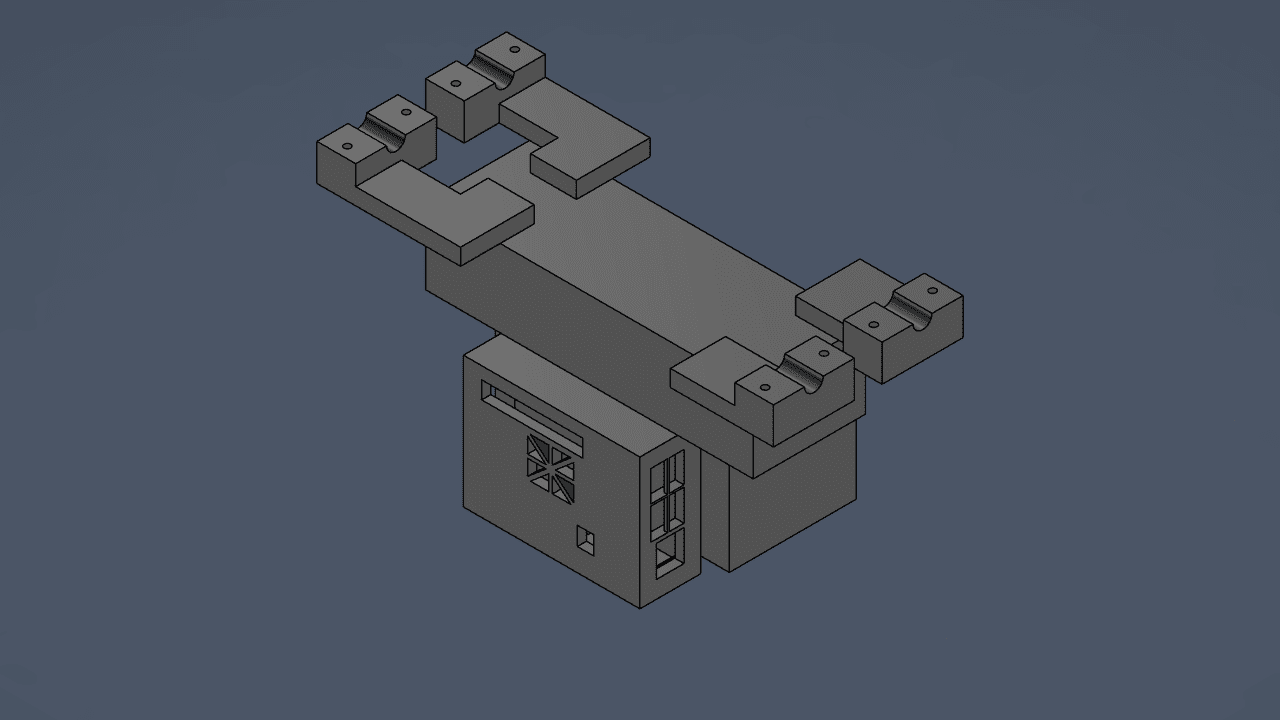
\includegraphics[width=0.9\linewidth]{bab3/dudukan_utama_kompartemen_3d_1}
		\caption{Desain 3D Dudukan Utama Kompartemen 1 (Desain Awal)}
		\label{fig:dudukan-utama-kompartemen-3d-1}
	\end{subfigure}
	\hfill
	\begin{subfigure}[b]{0.45\textwidth}
		\centering
		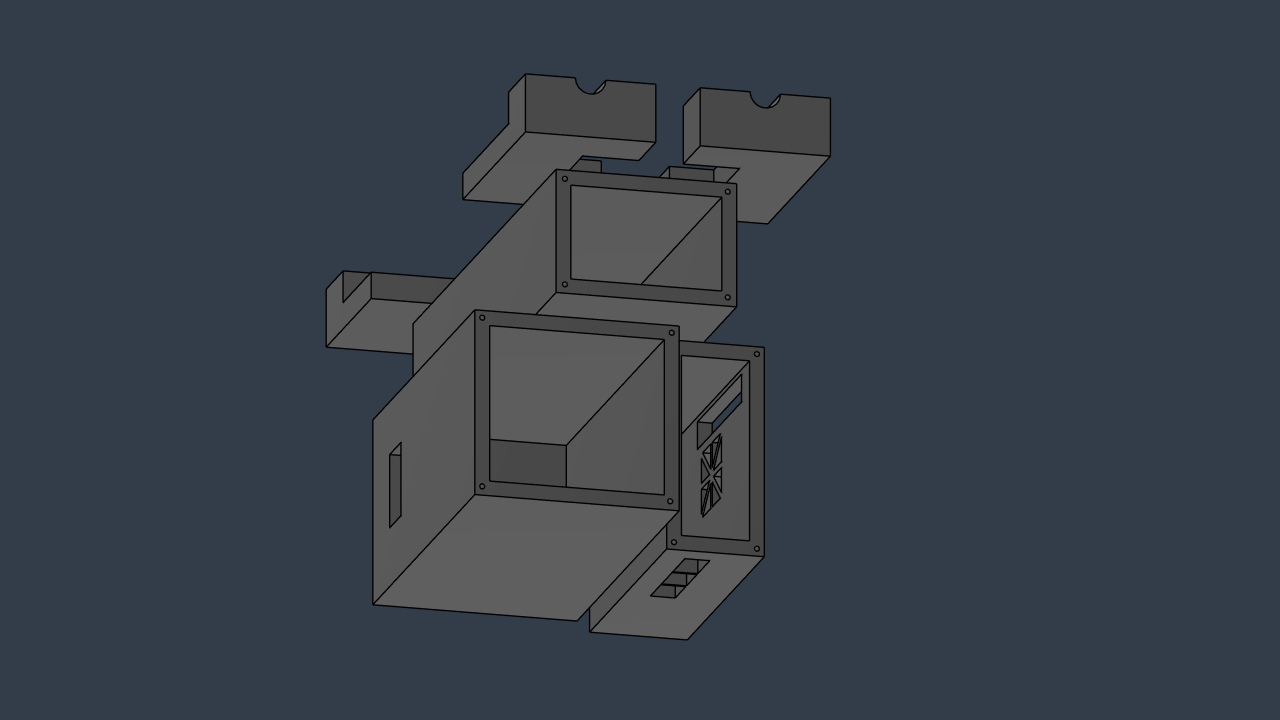
\includegraphics[width=0.9\linewidth]{bab3/dudukan_utama_kompartemen_3d_2}
		\caption{Desain 3D Dudukan Utama Kompartemen 2 (Desain Awal)}
		\label{fig:dudukan-utama-kompartemen-3d-2}
	\end{subfigure}
	\caption{Assembly CAD Kompartemen Utama (Desain Awal)}
\end{figure}

Gambar \ref{fig:dudukan-utama-kompartemen-3d-1} menunjukkan assembly CAD kompartemen utama pada Desain Awal. Karakteristik utama dari rancangan awal ini adalah sebagian besar komponen pelindung dirancang menyatu secara fisik dalam satu dudukan besar, menggunakan casing power supply terpisah untuk wadah modul regulator daya, serta dicetak menggunakan densitas infill sebesar 30\% dengan pola grid. Hal ini berdampak pada bobot wahana yang menjadi relatif berat dan menyulitkan proses pemeliharaan atau modifikasi secara individual. Kekurangan utama dari Desain Awal ini meliputi:
\begin{itemize}
	\item Bobot kompartemen yang terlalu berat menghambat efisiensi daya terbang drone.
	\item Struktur non-modular menyulitkan pembongkaran salah satu komponen elektronik jika terjadi kerusakan.
	\item Casing power supply terpisah memakan ruang berlebih di bawah rangka drone.
\end{itemize}

\subsubsection{Revisi dan Iterasi Desain Mekanik}
Setelah proses integrasi kelistrikan selesai dan pengujian membuktikan kebutuhan kestabilan catu daya, struktur mekanik drone direvisi secara komprehensif menjadi desain modular yang lebih efisien (Desain Final Iterasi 1). Revisi desain mekanik ini dipicu oleh perubahan arsitektur kelistrikan wahana, di mana sistem penyedia daya untuk Raspberry Pi 5 yang awalnya menggunakan unit power supply dengan casing terpisah digantikan oleh converter UBEC 5A yang lebih ringkas. Perubahan sistem kelistrikan ini memungkinkan penghilangan casing power supply terpisah pada kompartemen. Ruang kosong yang ditinggalkan kemudian dialokasikan untuk menempatkan Casing modem, yang mana modem tersebut sangat dibutuhkan untuk menunjang konektivitas terbang (komunikasi data telemetri dan kontrol) ke operator.

Perubahan utama pada Desain Final Iterasi 1 ini meliputi:
\begin{itemize}
	\item Desain ulang komponen menjadi beberapa unit mekanik modular terpisah, yaitu Casing baterai, Tutup casing baterai, Casing modem, Tutup casing modem, Casing Raspberry Pi, Tutup casing Raspberry Pi, Casing kamera, Tutup kamera, Tutup clamp depan, serta Tutup clamp belakang.
	\item Penghilangan casing power supply terpisah dan pengalokasian ruang kosong untuk Casing modem.
	\item Pengurangan densitas pencetakan menjadi infill 10\% dengan menerapkan pola cetak Gyroid untuk meminimalkan bobot tanpa mengorbankan kekuatan struktural.
\end{itemize}

Berikut adalah visualisasi Assembly CAD Desain Final Iterasi 1 yang menunjukkan penataan komponen modular secara keseluruhan dari dua sudut pandang berbeda:

\begin{figure}[H]
	\centering
	\begin{subfigure}[b]{0.45\textwidth}
		\centering
		\includegraphics[width=\linewidth]{bab3/desain2final}
		\caption{Tampak Perspektif 1}
	\end{subfigure}
	\hfill
	\begin{subfigure}[b]{0.45\textwidth}
		\centering
		\includegraphics[width=\linewidth]{bab3/desain2final2}
		\caption{Tampak Perspektif 2}
	\end{subfigure}
	\caption{Assembly CAD Desain Final Iterasi 1}
	\label{fig:desain2final}
\end{figure}

\subsubsection{Penyempurnaan Akhir (Refinement / Iterasi 2)}
Meskipun desain modular telah diterapkan pada Iterasi 1, pengujian awal penerbangan menunjukkan masih terdapat beberapa kelemahan mekanik sehingga dilakukan penyempurnaan (refinement) terhadap beberapa komponen tanpa mengubah arsitektur keseluruhan sistem. Perubahan hasil iterasi refinement meliputi:
\begin{itemize}
	\item Casing baterai: Penggabungan konektor dudukan ke frame drone langsung ke bodi casing agar tidak rentan patah saat landing.
	\item Casing kamera: Penambahan area kontak dan penyesuaian celah toleransi agar webcam Logitech C922 tidak bergeser sudut inklinasinya akibat vibrasi motor drone.
	\item Tutup kamera: Penyempurnaan mekanisme ulir baut penegang untuk penjepitan bodi kamera yang lebih merata.
\end{itemize}

\subsubsection{Assembly Final dan Realisasi Fisik}
Setelah seluruh komponen modular disempurnakan pada tahap refinement, integrasi akhir dirancang dalam bentuk assembly CAD final yang siap diimplementasikan secara fisik pada wahana drone.

\begin{figure}[H]
	\centering
	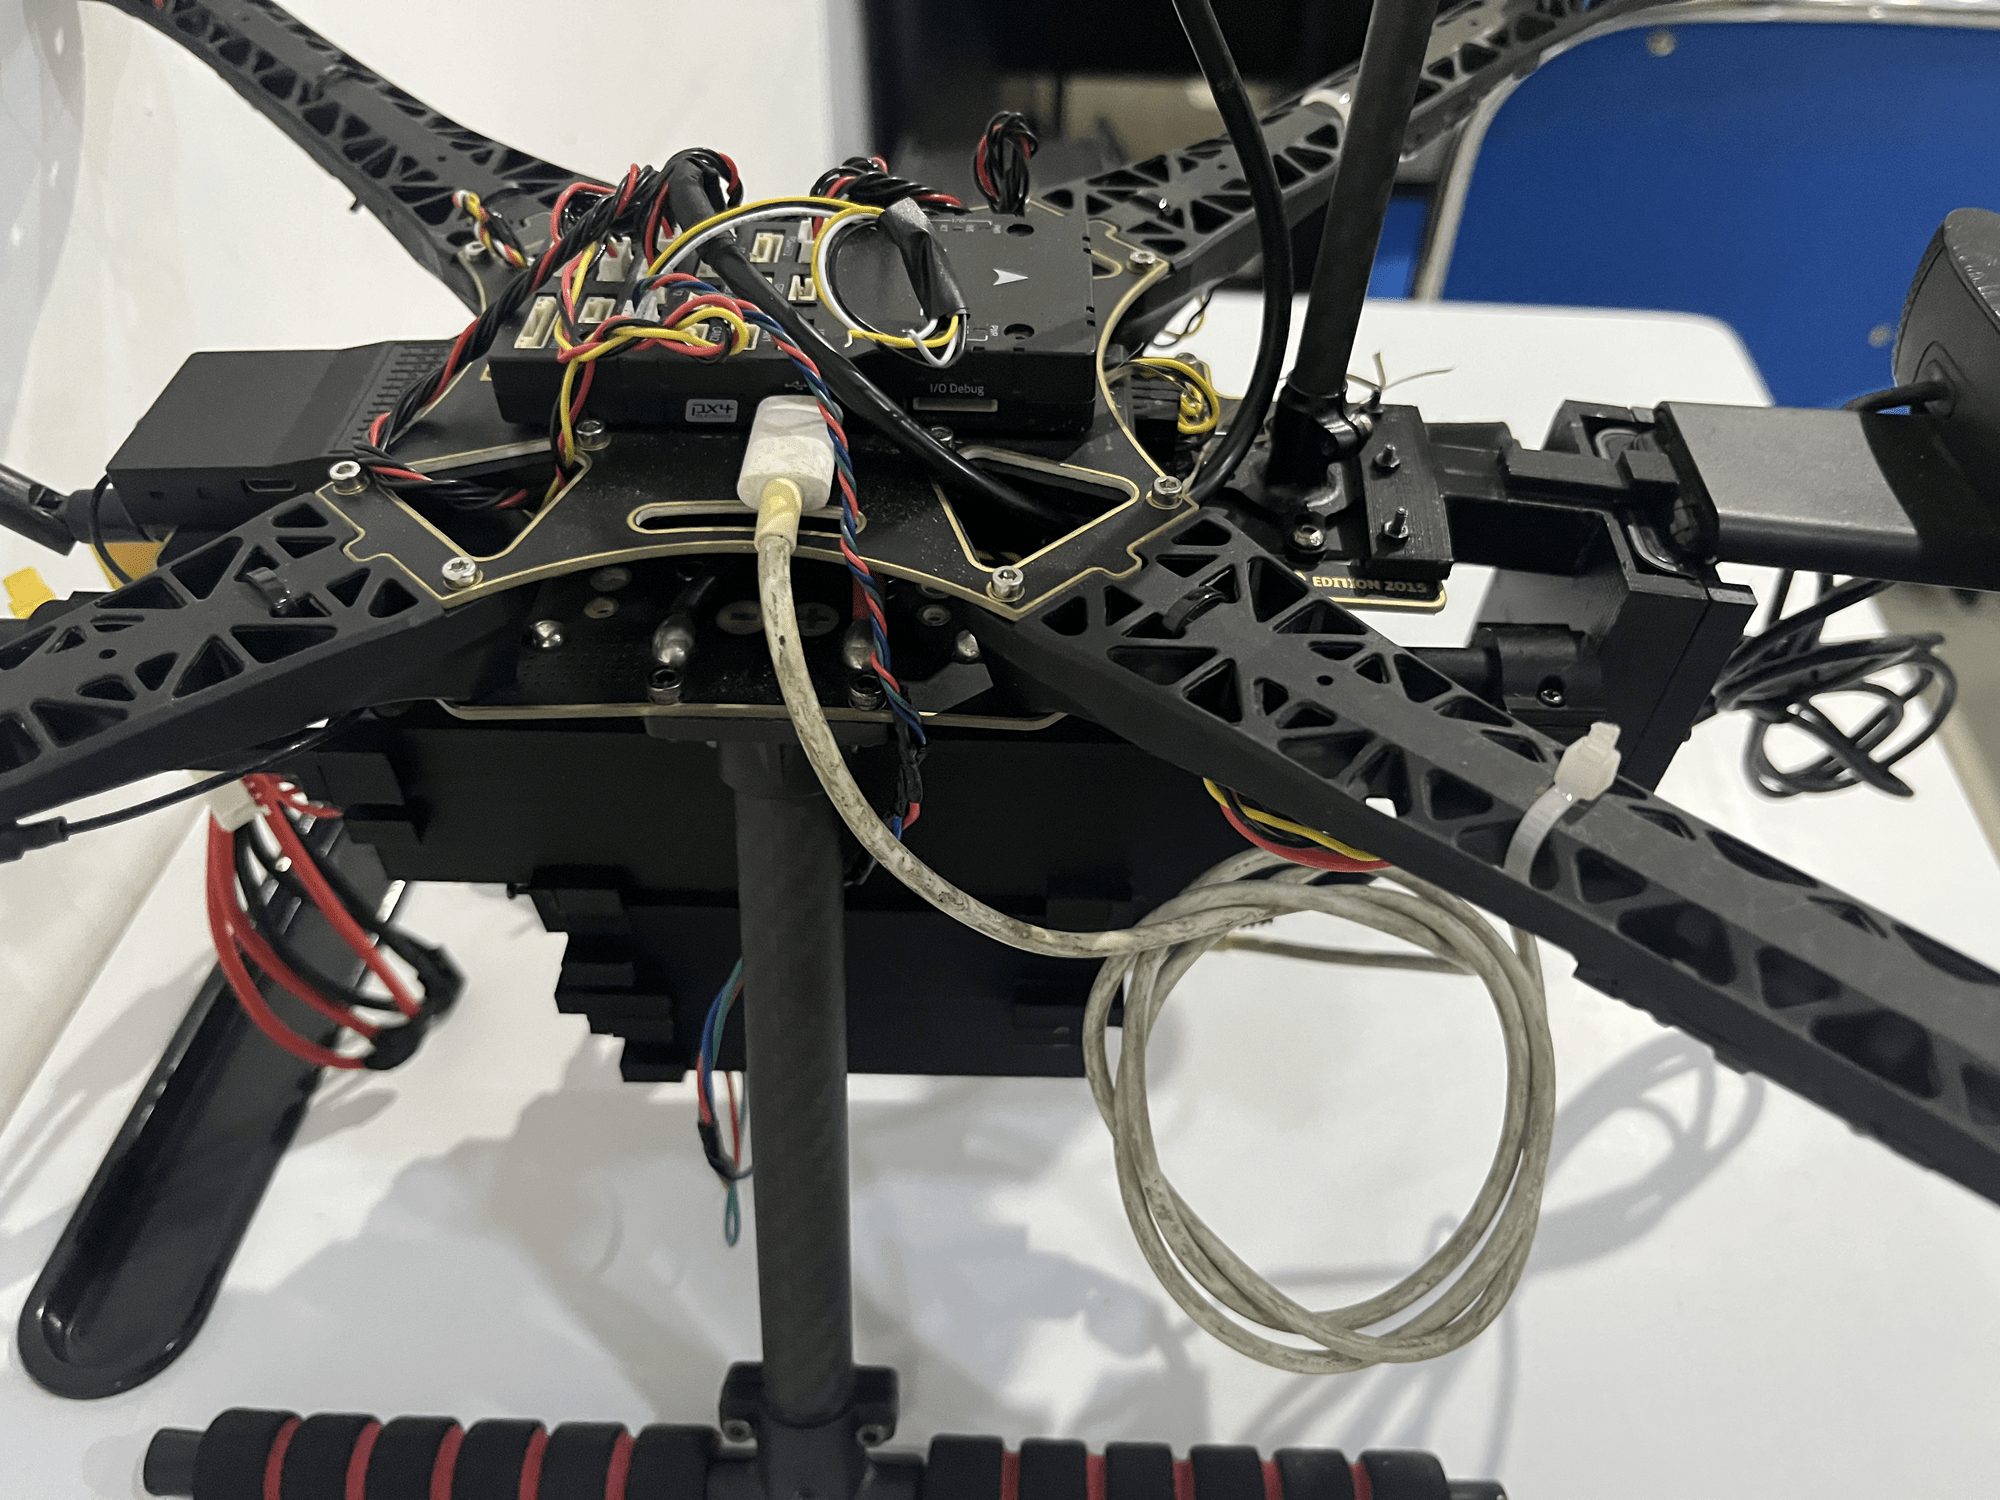
\includegraphics[width=0.8\linewidth]{bab3/tampak_samping_manajemen_kabel}
	\caption{Assembly CAD Desain Final Tampak Samping}
	\label{fig:tampak_samping_usb_baru}
\end{figure}

Gambar \ref{fig:tampak_samping_usb_baru} menunjukkan assembly CAD dari keseluruhan sistem mekanik penunjang otonom drone. Terlihat bahwa seluruh komponen modular terpasang secara simetris di bagian tengah bawah wahana untuk menjaga keselarasan titik berat drone.

\begin{figure}[H]
	\centering
	\begin{subfigure}[b]{0.45\textwidth}
		\centering
		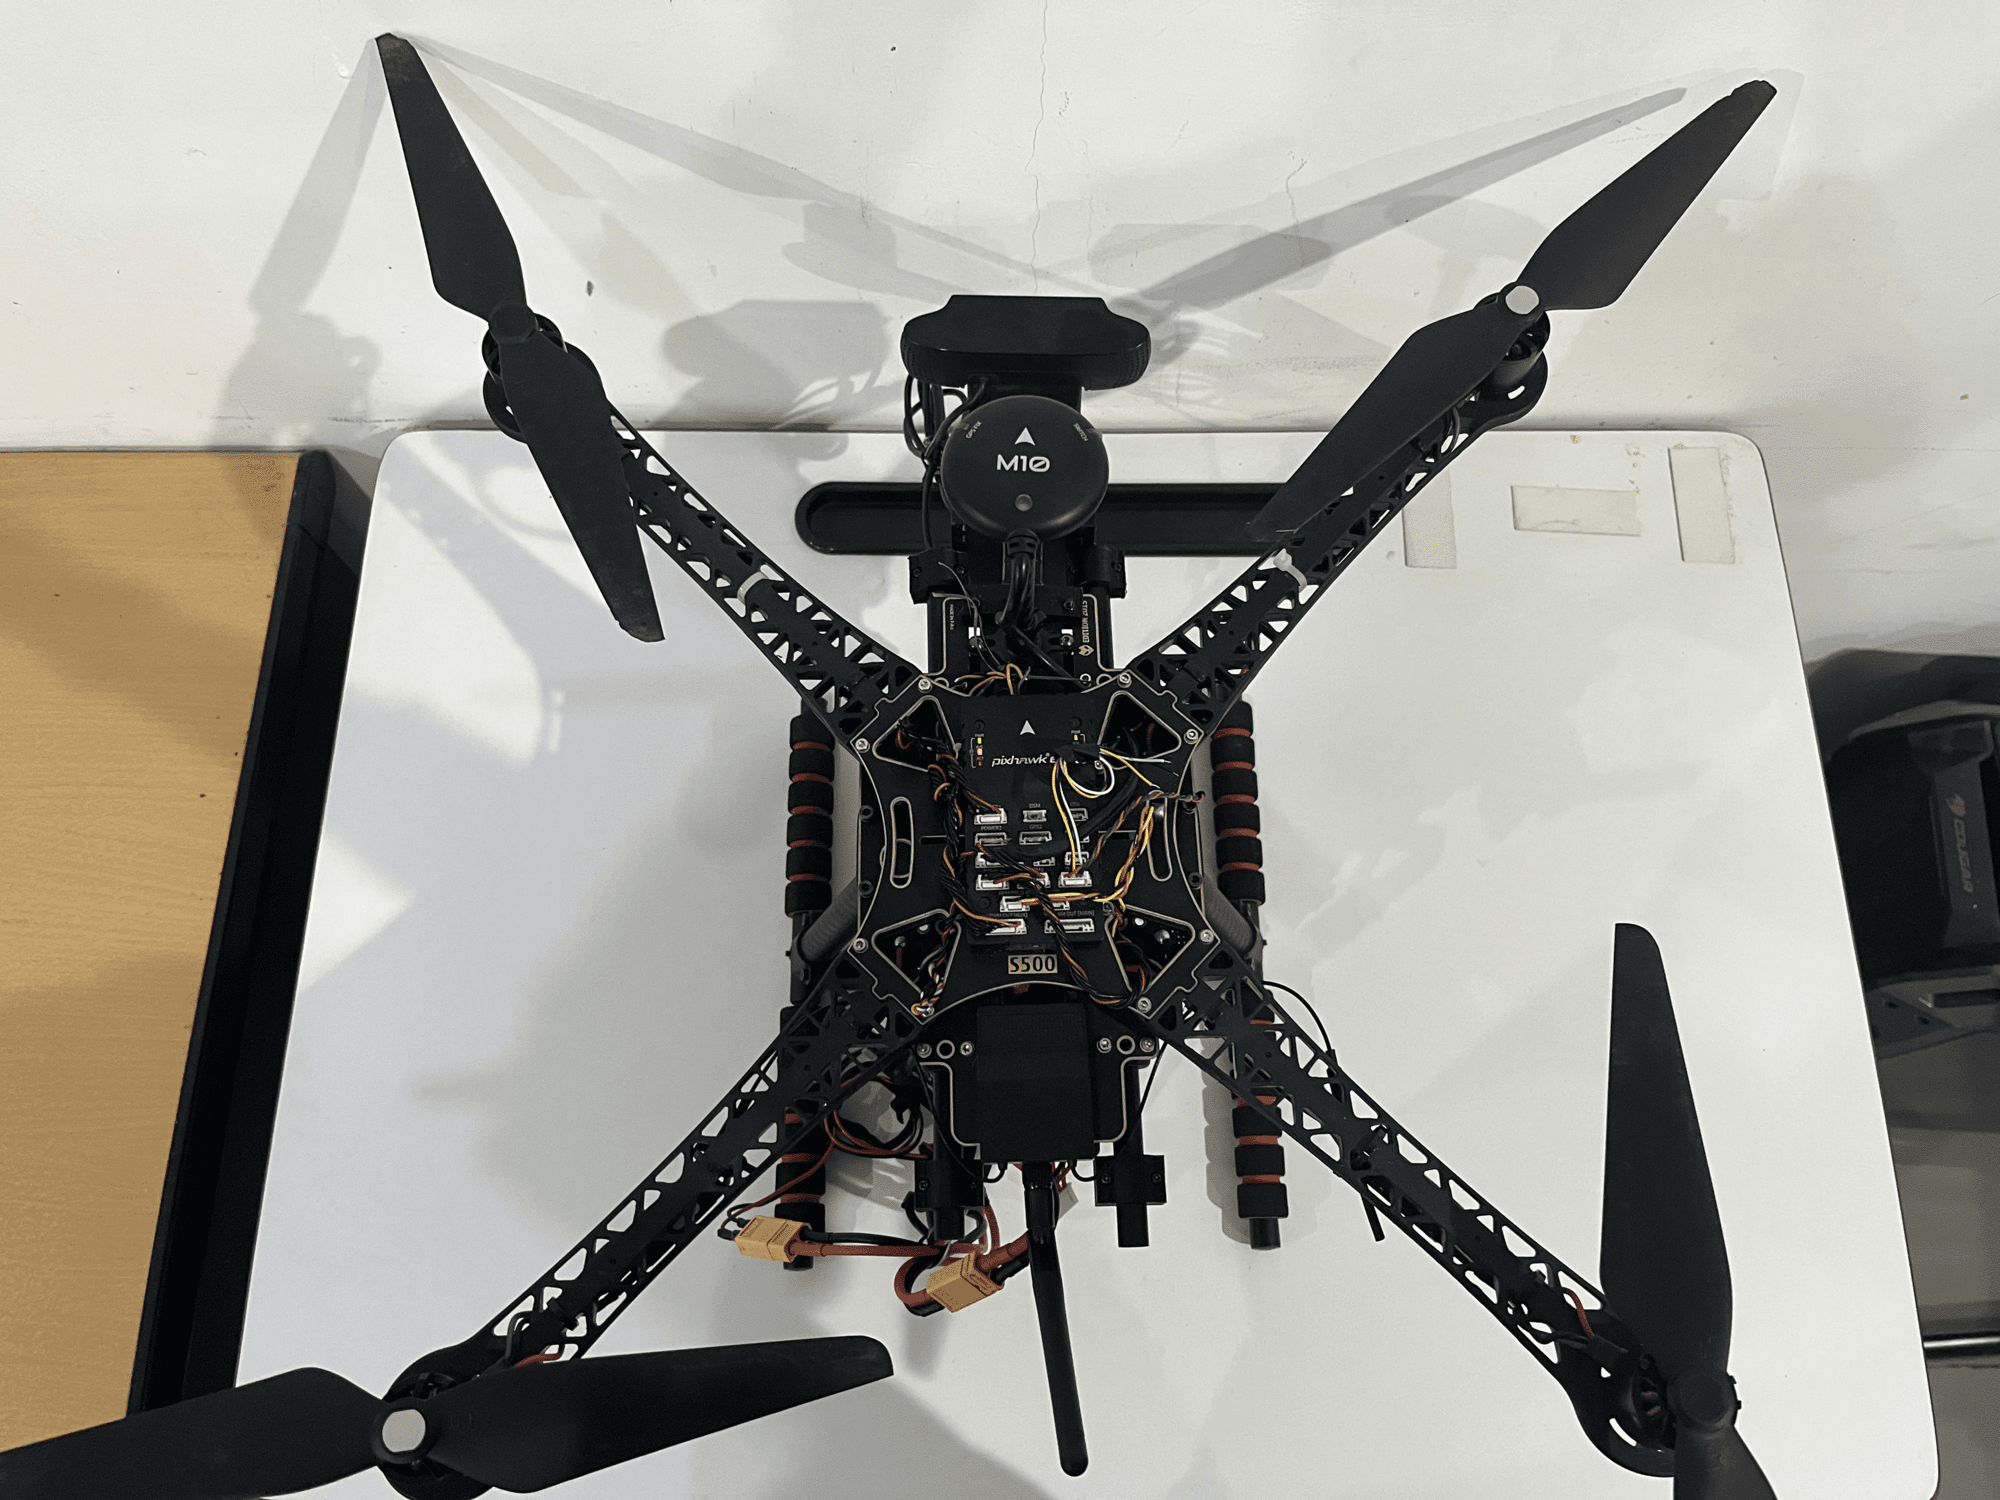
\includegraphics[width=\linewidth]{bab3/IMG_1258}
		\caption{Hasil Realisasi Perakitan Final Tampak Perspektif 1}
	\end{subfigure}
	\hfill
	\begin{subfigure}[b]{0.45\textwidth}
		\centering
		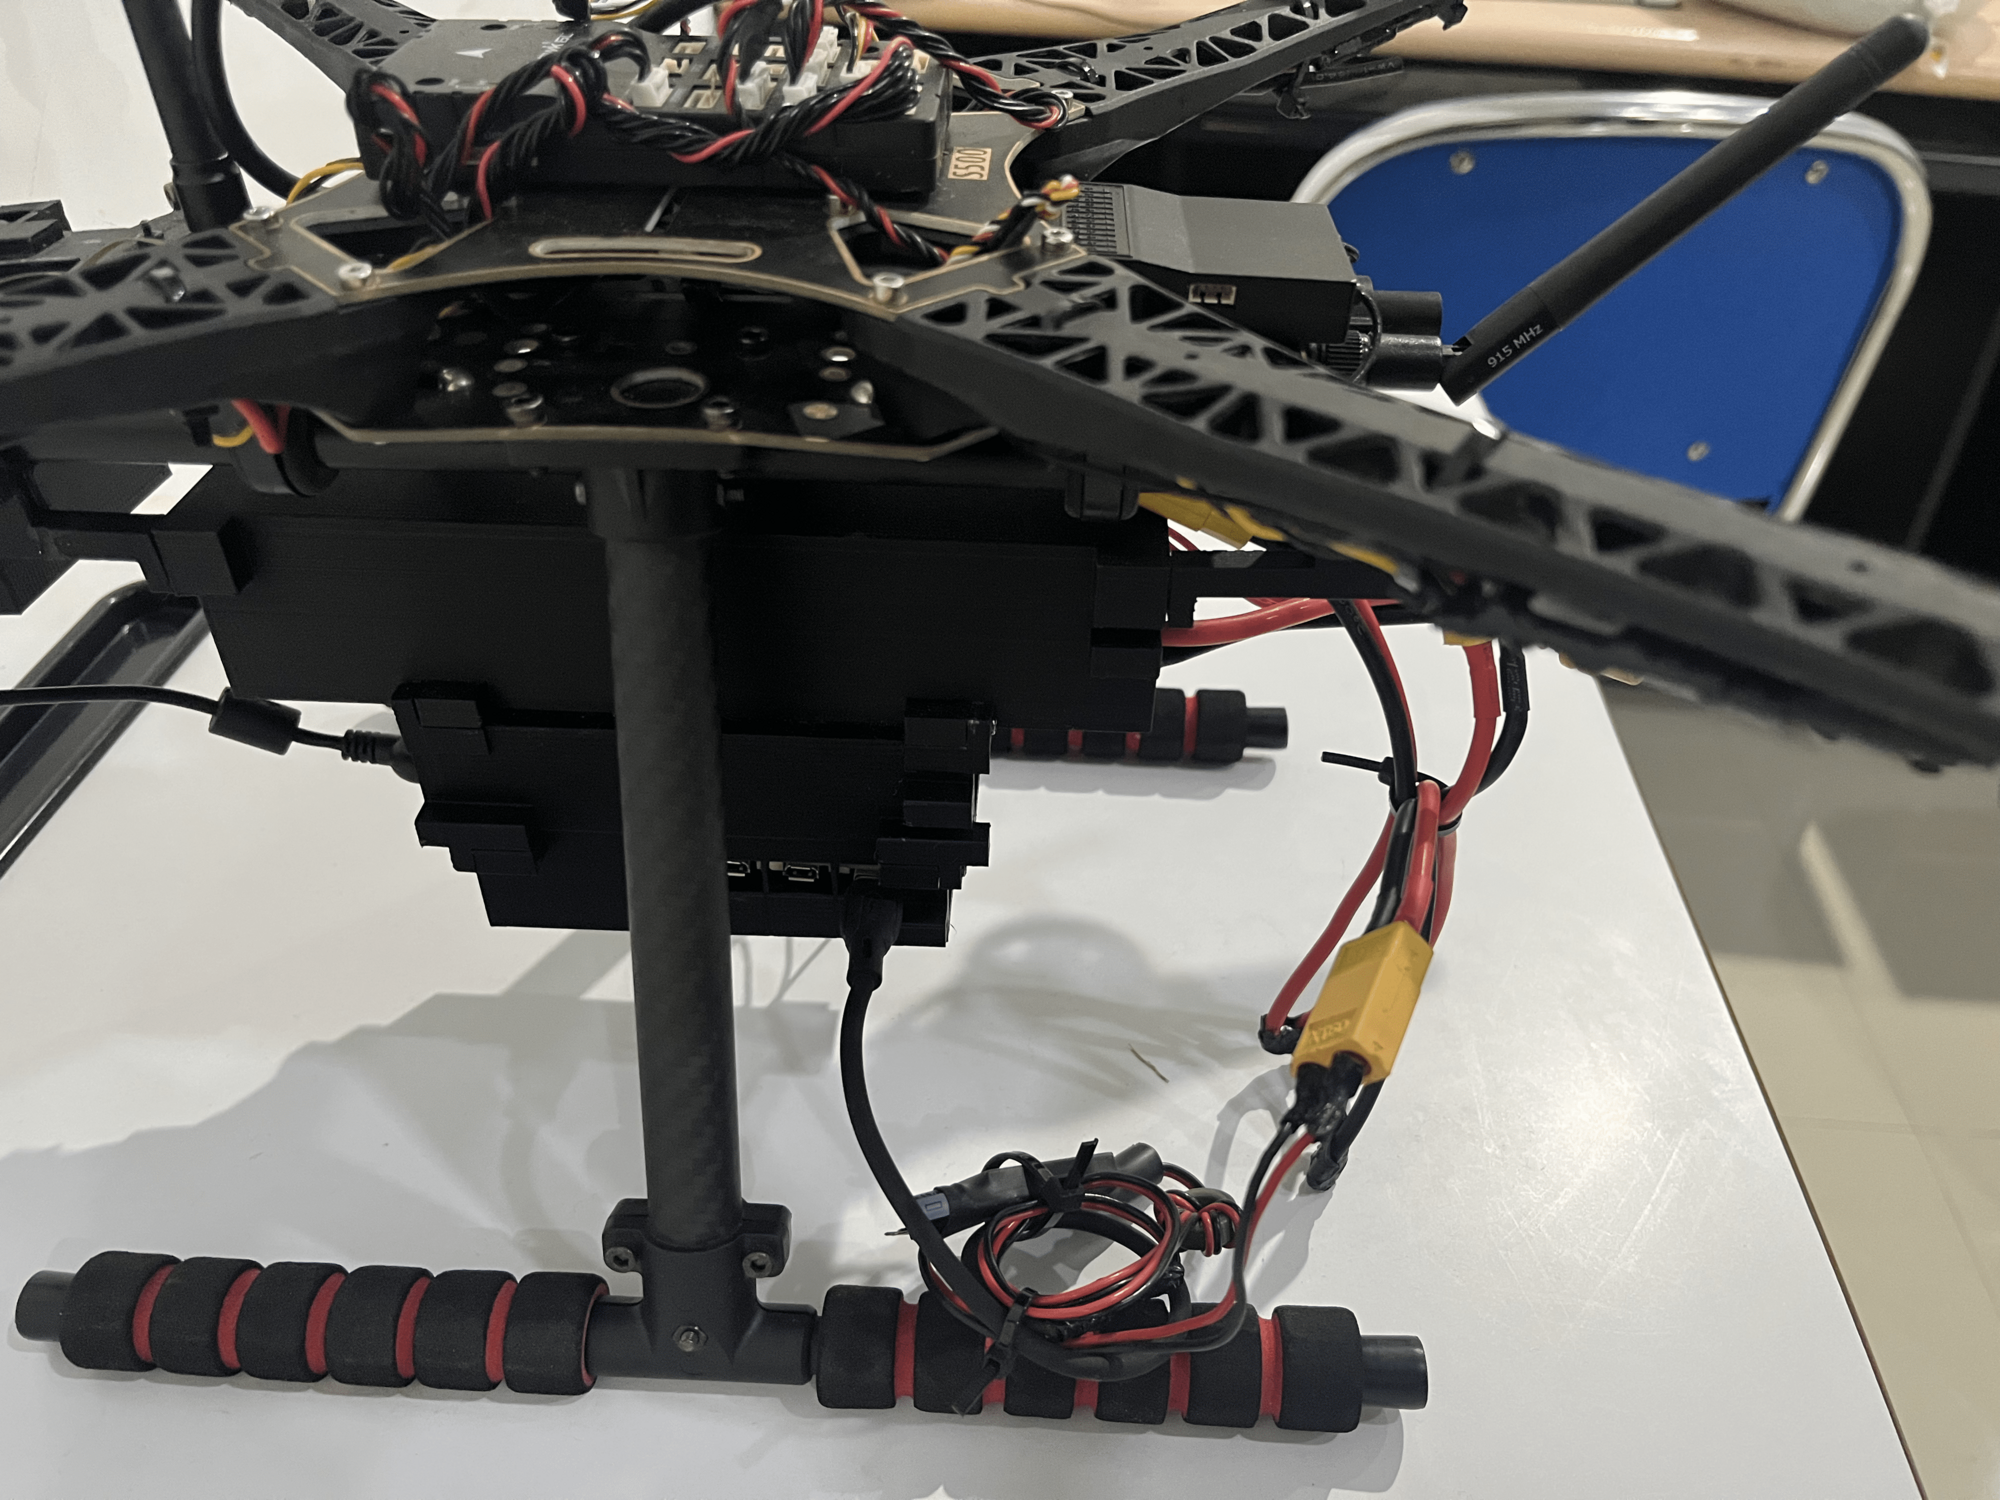
\includegraphics[width=\linewidth]{bab3/IMG_1268}
		\caption{Hasil Realisasi Perakitan Final Tampak Perspektif 2}
	\end{subfigure}
	\caption{Realisasi Fisik Perakitan Keseluruhan Sistem (Desain Final)}
	\label{fig:perakitan_final_real}
\end{figure}

Gambar \ref{fig:perakitan_final_real} menunjukkan hasil realisasi perakitan fisik dari keseluruhan sistem drone berdasarkan desain final yang dirancang. Berdasarkan implementasi tersebut, seluruh komponen cetak 3D telah terpasang secara kokoh pada rangka Holybro S500. Dapat diamati bahwa konfigurasi ini menghasilkan struktur yang ringkas dengan pusat massa yang terdistribusi secara seimbang. Dengan demikian, realisasi fisik drone ini telah siap digunakan sebagai platform uji coba penerbangan otonom. Komponen Casing baterai yang terpasang pada bagian bawah rangka tersebut telah menggunakan rancangan dengan Konektor dudukan ke frame drone terintegrasi untuk menjamin kekuatan struktural wahana.

\subsubsection{Rincian Detail Komponen Mekanik (Desain Final)}
Berikut adalah visualisasi rinci dari masing-masing komponen mekanik modular hasil cetakan final, yang meliputi model CAD 3D, gambar teknik 2D, serta foto realisasi fisiknya:

\paragraph{Casing Baterai}
\begin{figure}[H]
	\centering
	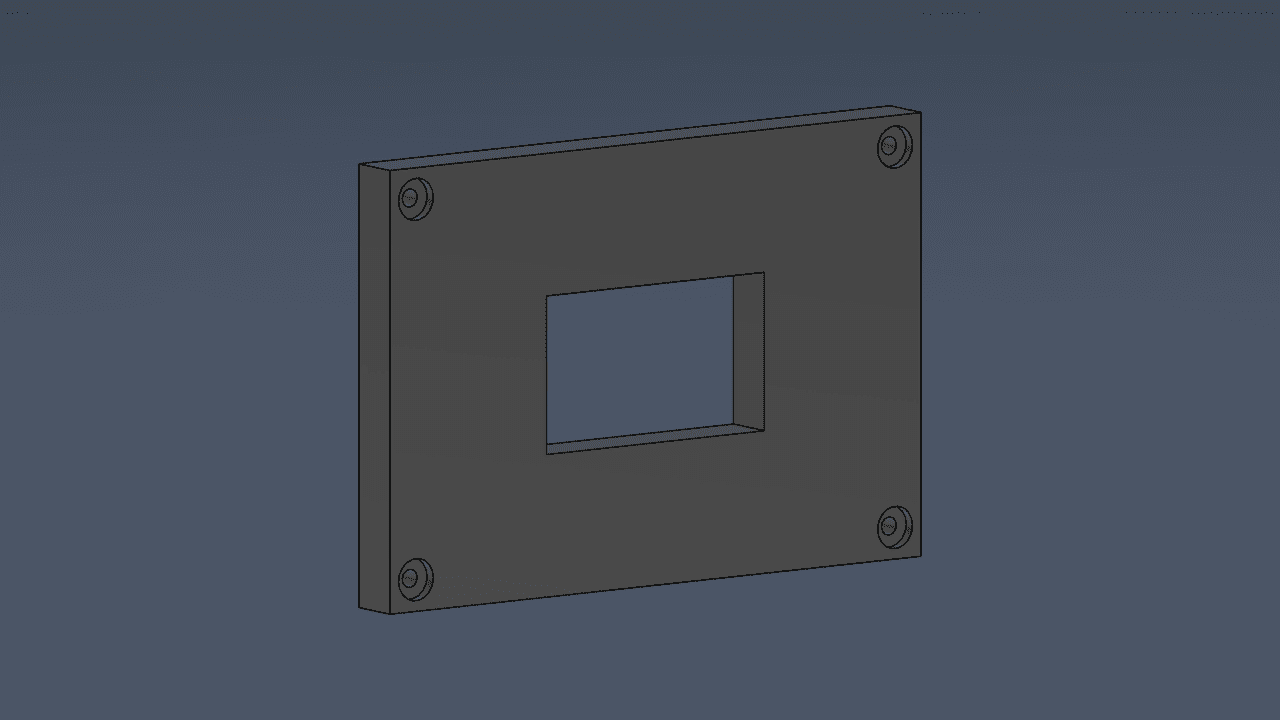
\includegraphics[width=0.7\linewidth]{bab3/casing_baterai_3d_1}
	\caption{CAD Desain Sebelum Revisi (Casing Baterai)}
	\label{fig:casing-baterai-awal-3d-1}
\end{figure}

\begin{figure}[H]
	\centering
	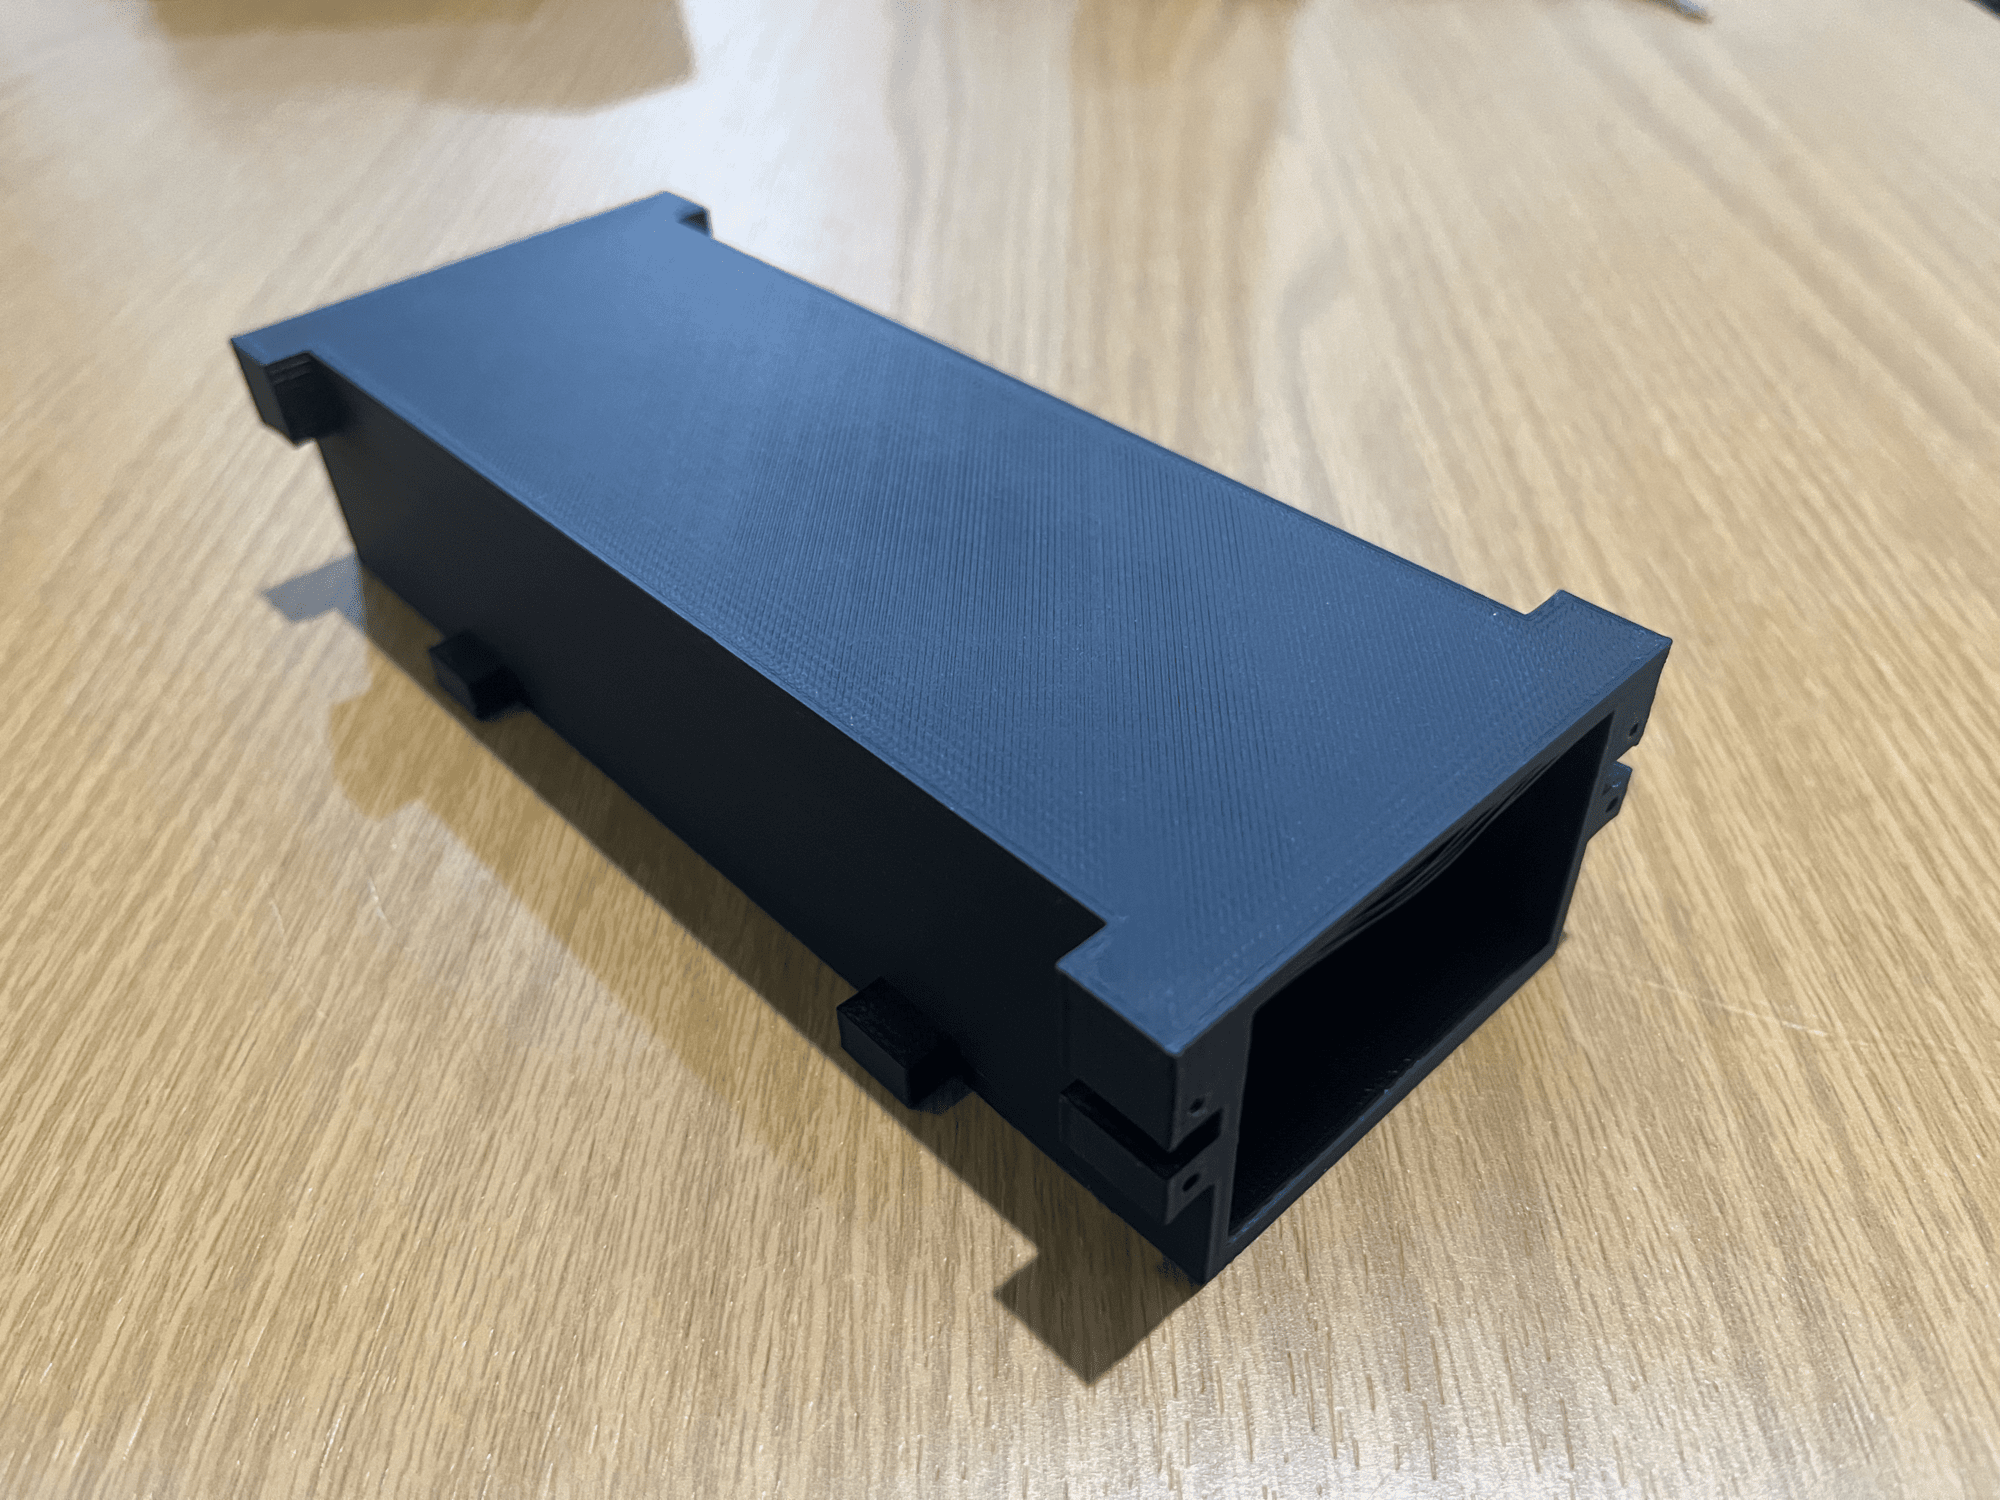
\includegraphics[width=0.7\linewidth]{bab3/casing_baterai}
	\caption{CAD Desain Setelah Revisi (Casing Baterai)}
	\label{fig:casing_baterai_baru}
\end{figure}

\begin{figure}[H]
	\centering
	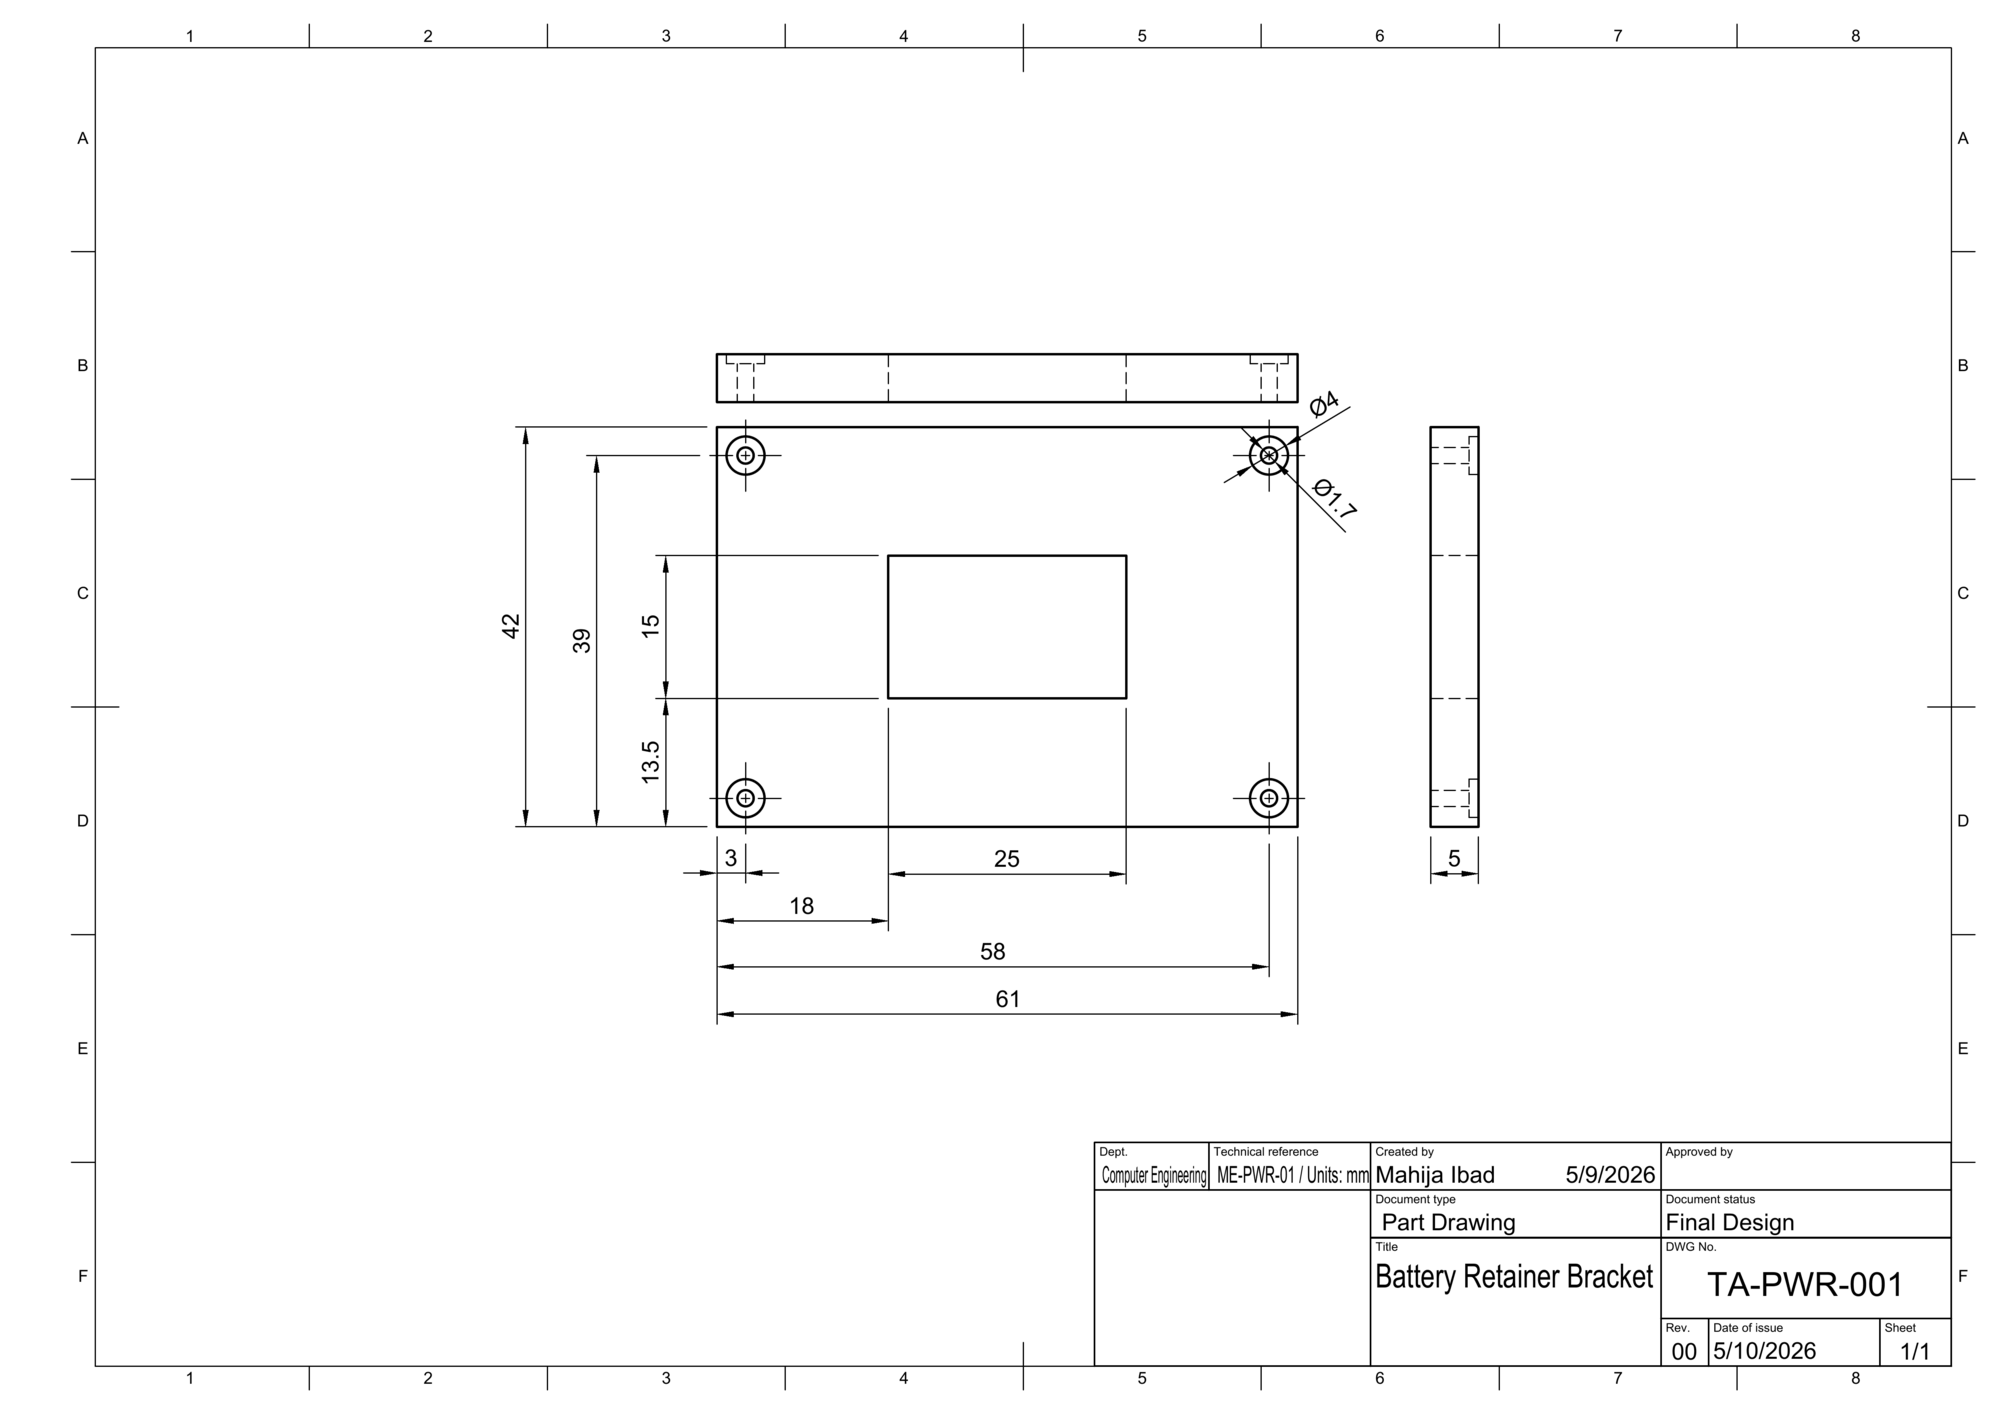
\includegraphics[width=0.7\linewidth]{bab3/casing_baterai_2d}
	\caption{Gambar Teknik (2D Drawing) Casing Baterai}
	\label{fig:casing-baterai-awal-2d}
\end{figure}

\begin{figure}[H]
	\centering
	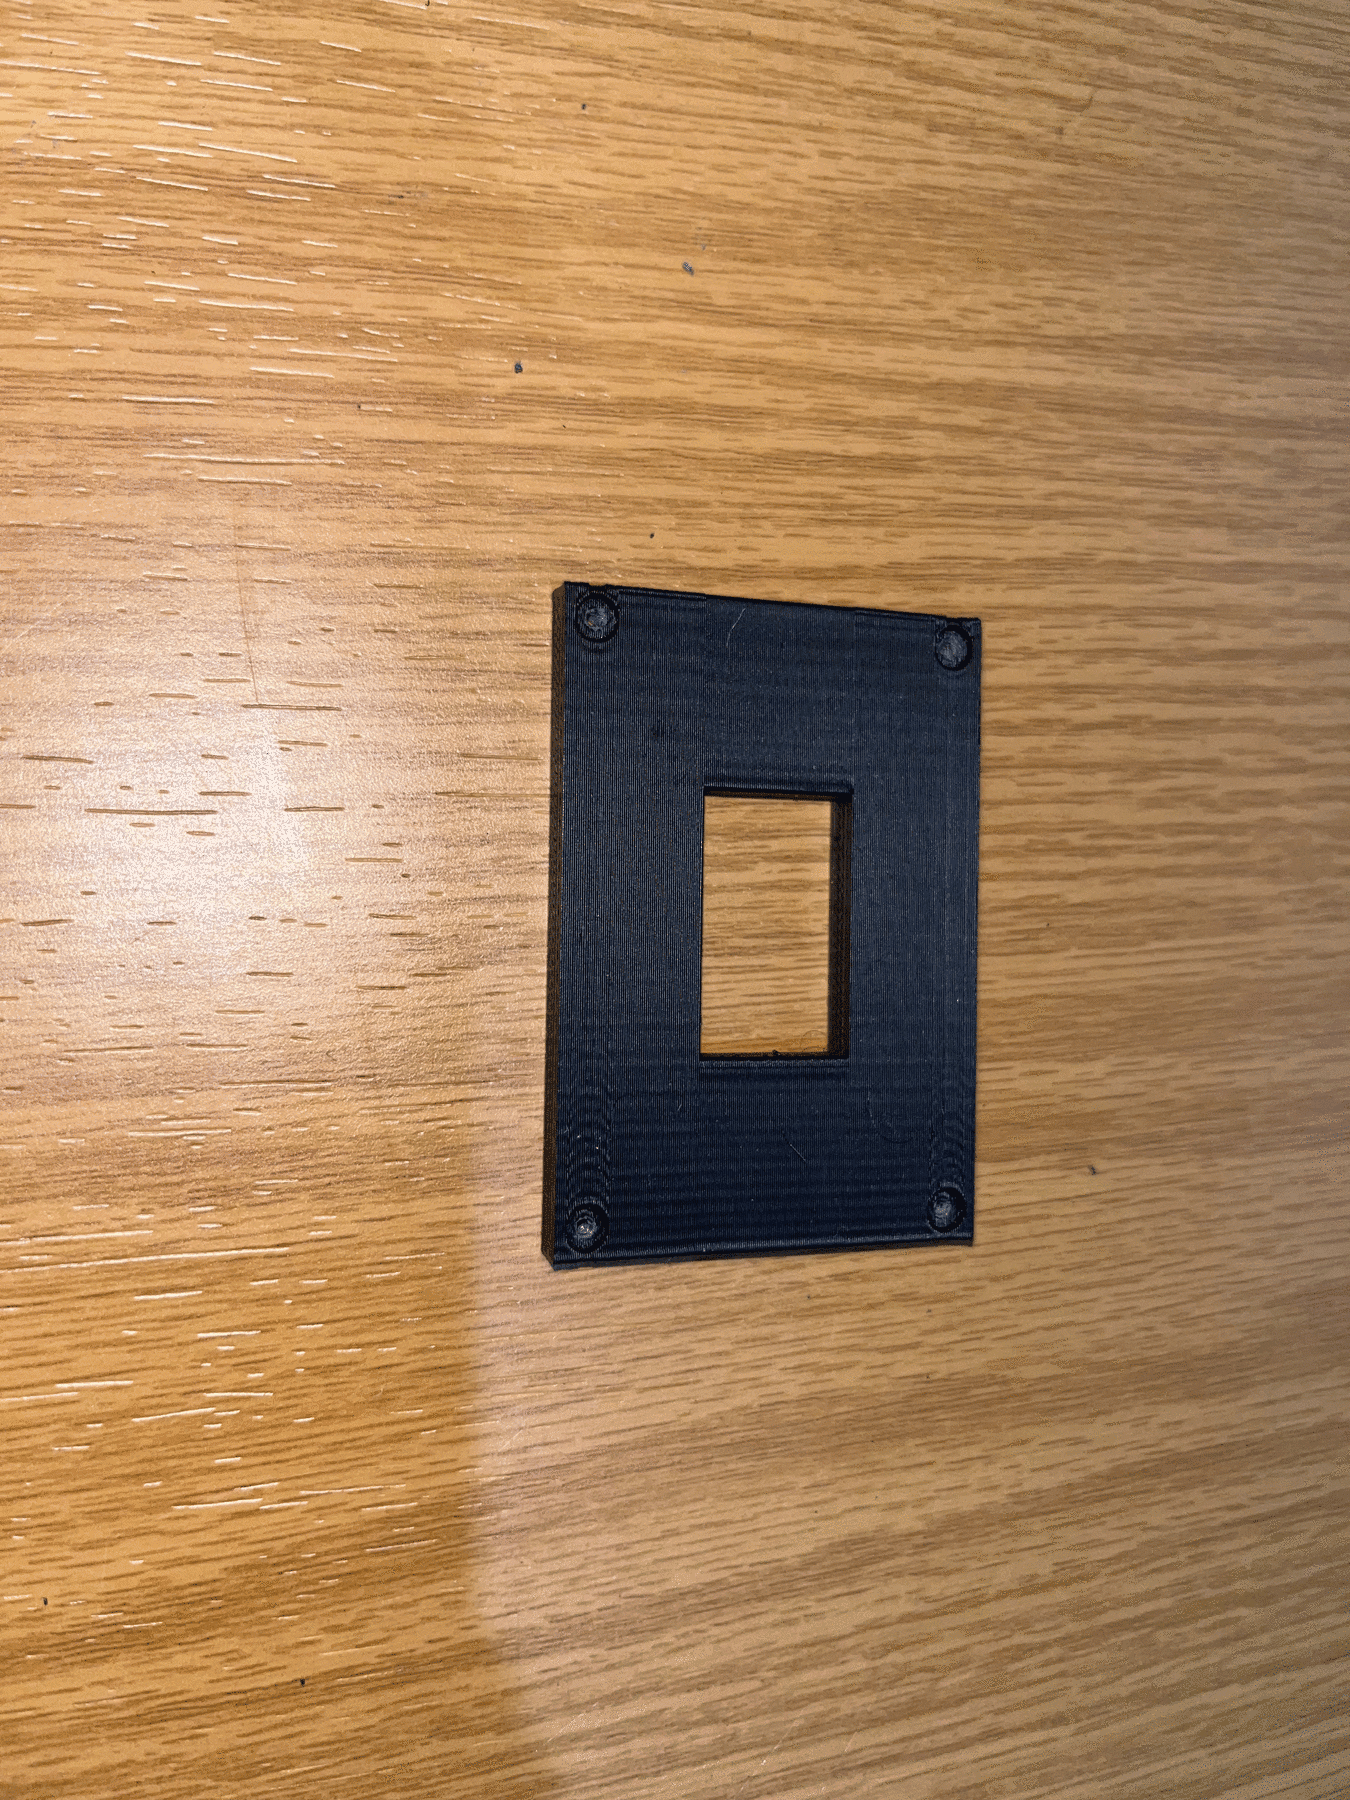
\includegraphics[width=0.7\linewidth]{bab3/casing_baterai_real1}
	\caption{Hasil Pencetakan / Implementasi Fisik Casing Baterai}
	\label{fig:retainer-baterai-real-1}
\end{figure}

Penyempurnaan pada komponen Casing baterai didorong oleh temuan selama pengujian lepas landas dan pendaratan. Sebelumnya pada Desain Final Iterasi 1, konektor dudukan ke frame drone dibuat secara terpisah dengan penampang yang relatif kecil. Akibatnya, konektor tersebut rentan mengalami patah ketika menahan beban baterai LiPo 4S seberat 500 gram saat terjadi benturan saat pendaratan. Sebagai langkah penyempurnaan (refinement) pada Desain Final Iterasi 2, konektor dudukan diintegrasikan secara menyatu dengan Casing baterai. Hal ini meningkatkan luas penampang melintang serta meningkatkan kekakuan mekanis struktur penopang.

\paragraph{Casing Kamera}
\begin{figure}[H]
	\centering
	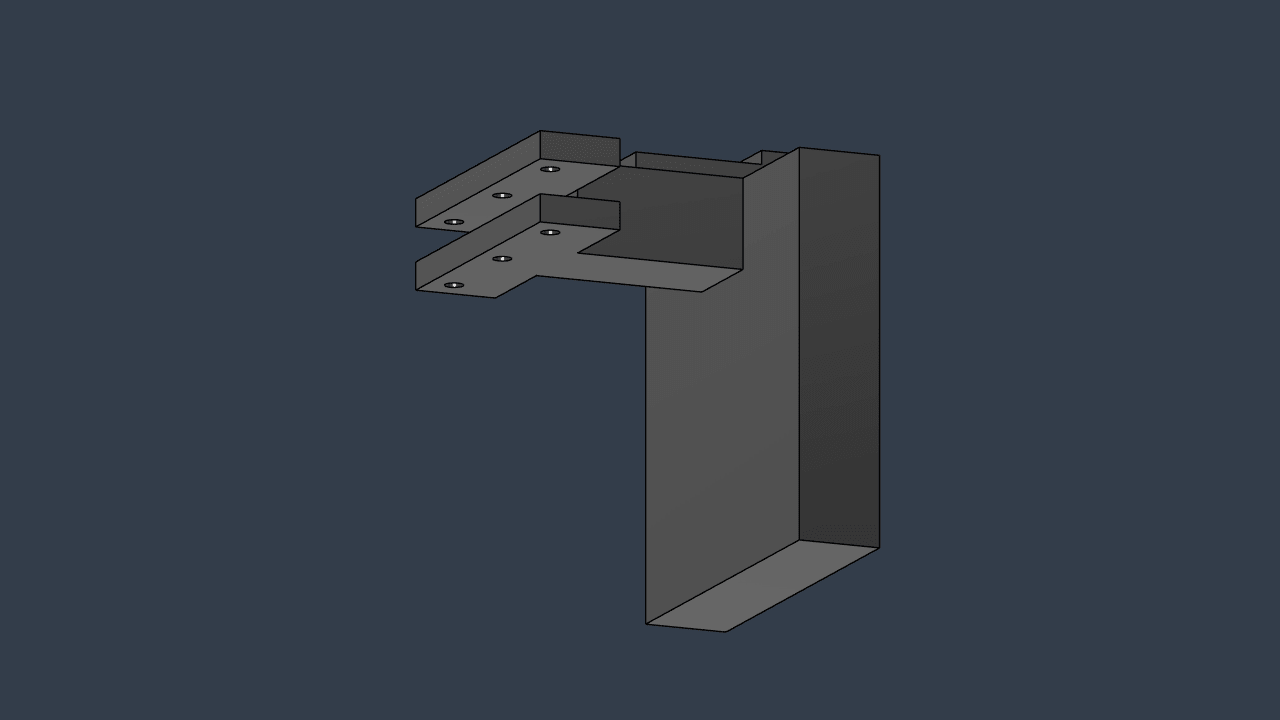
\includegraphics[width=0.7\linewidth]{bab3/casing_kamera_3d_1}
	\caption{CAD Desain Sebelum Revisi (Casing Kamera)}
	\label{fig:casing-kamera-awal-3d-1}
\end{figure}

\begin{figure}[H]
	\centering
	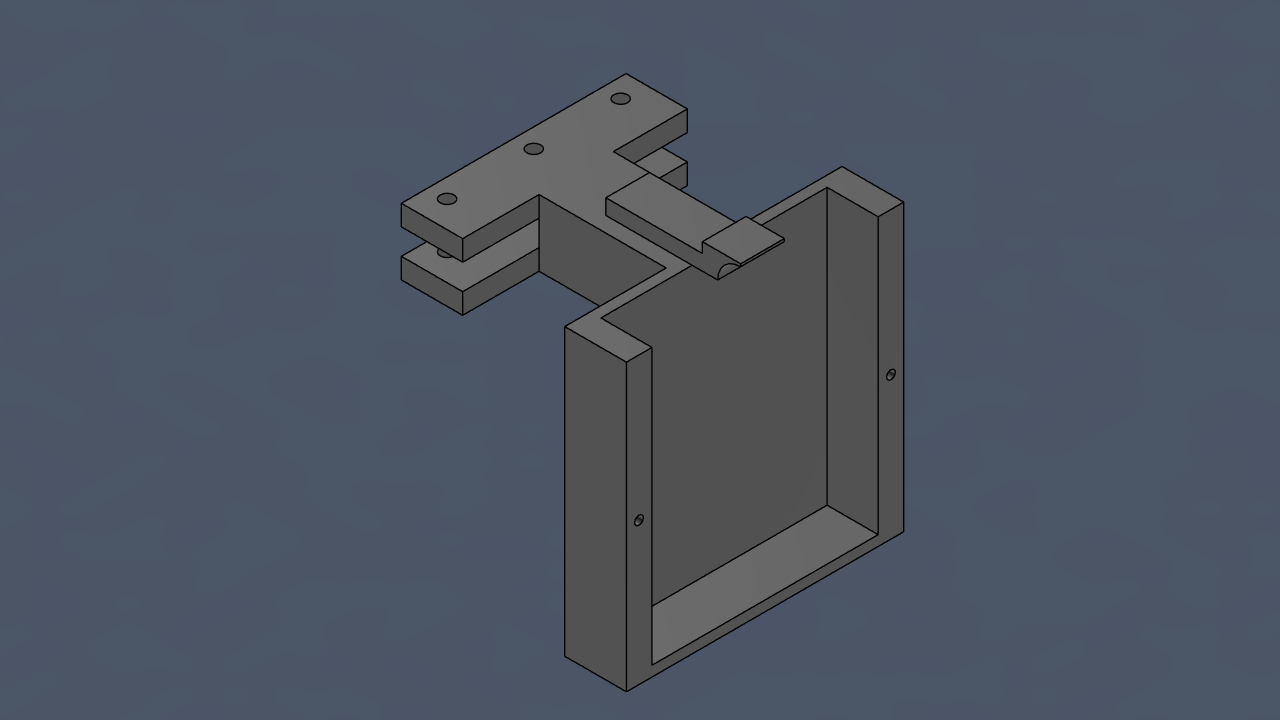
\includegraphics[width=0.7\linewidth]{bab3/casing_kamera_3d_2}
	\caption{CAD Desain Setelah Revisi (Casing Kamera)}
	\label{fig:casing-kamera-awal-3d-2}
\end{figure}

\begin{figure}[H]
	\centering
	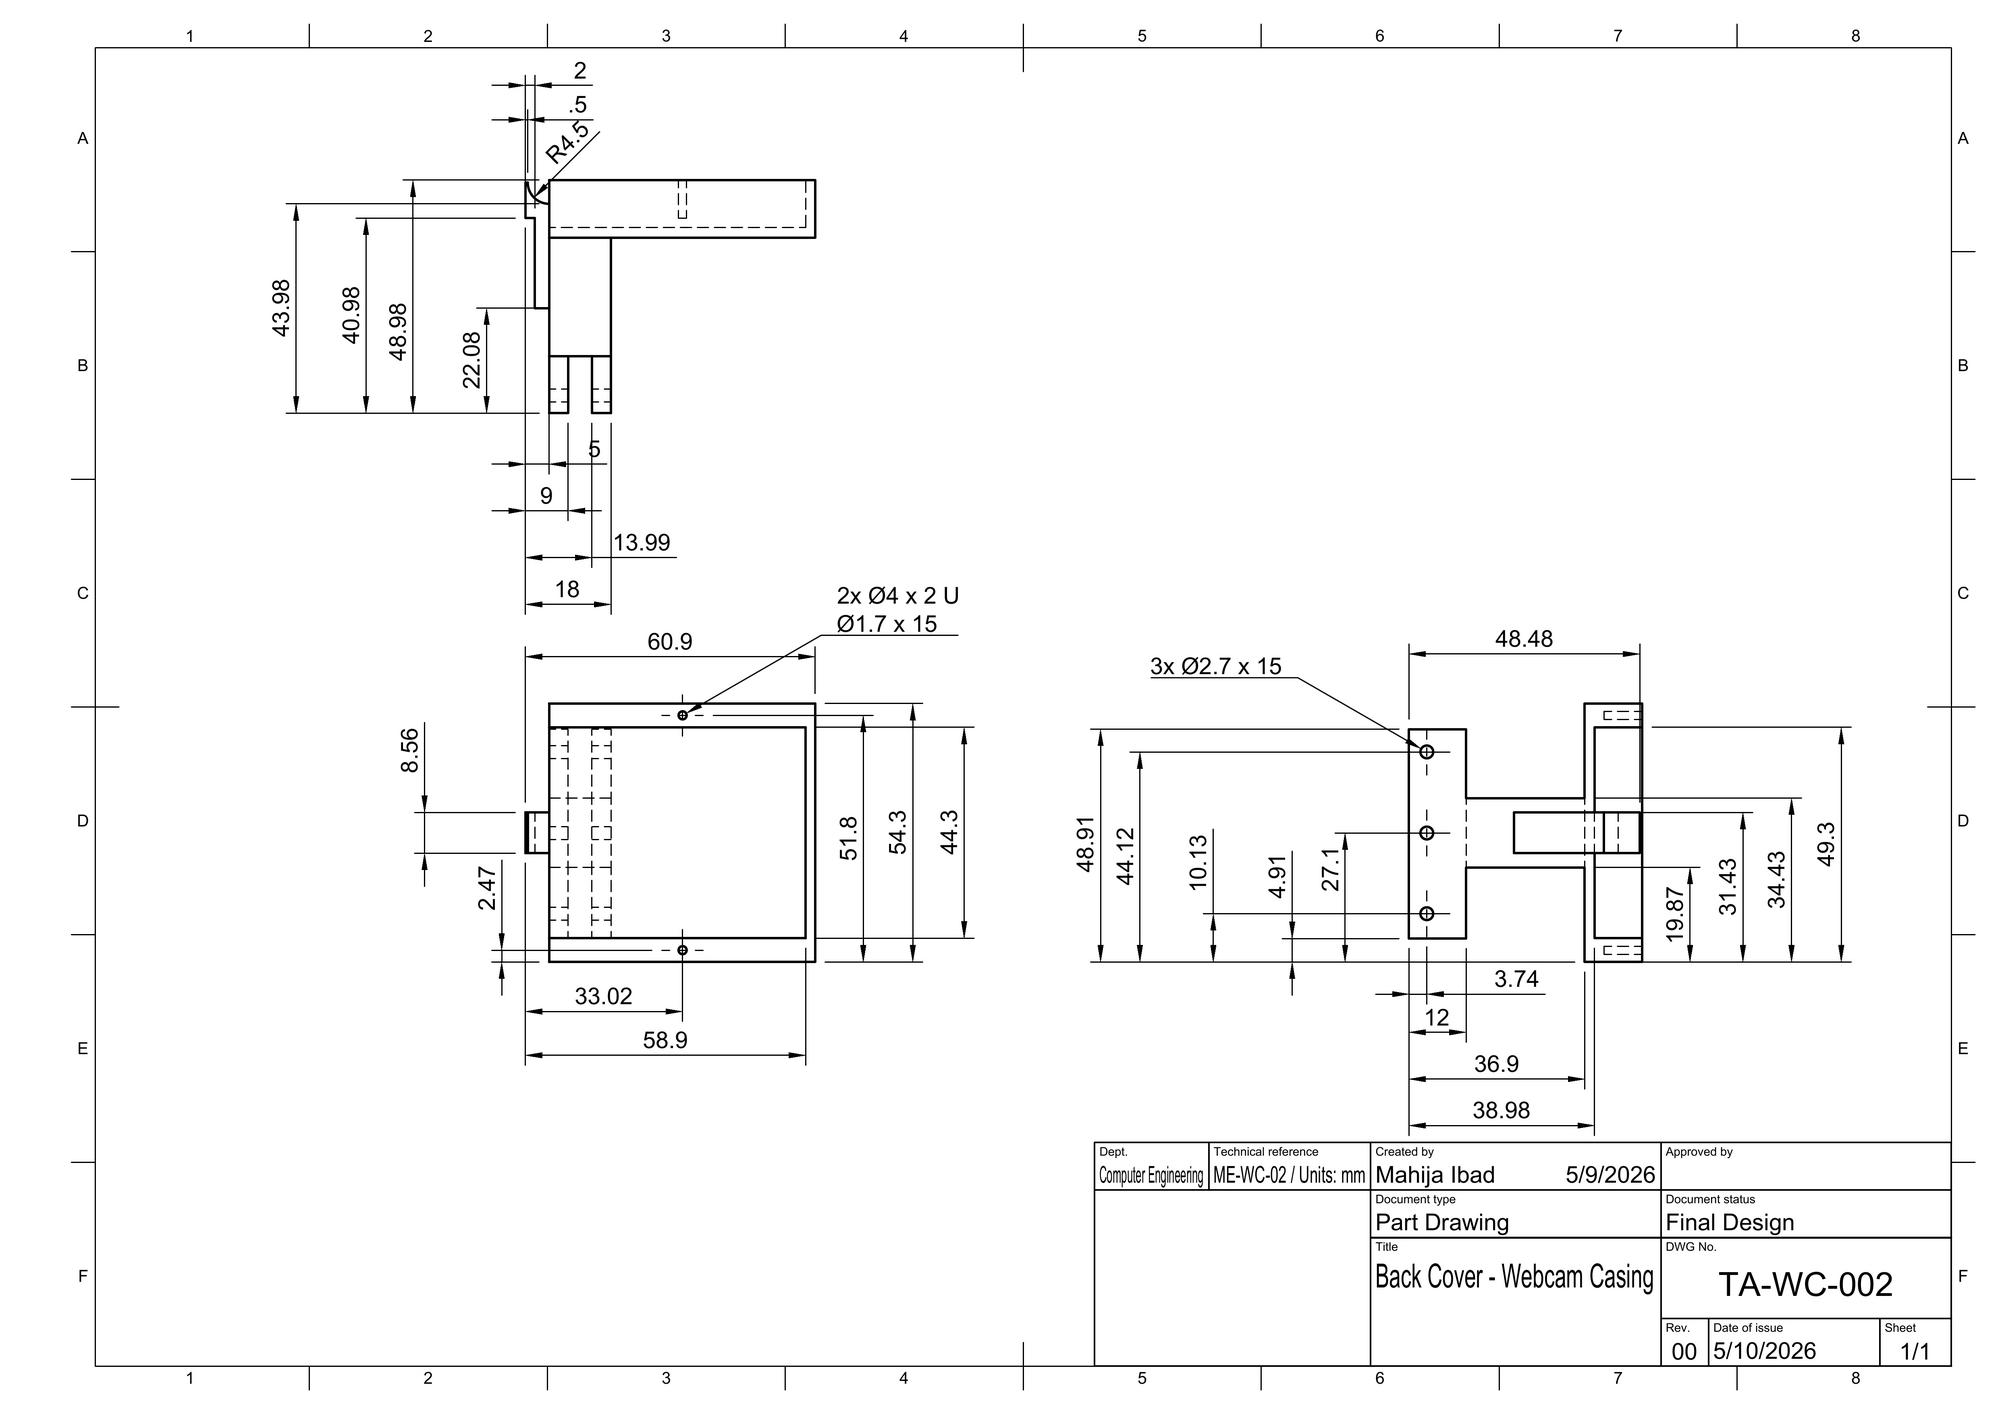
\includegraphics[width=0.7\linewidth]{bab3/casing_kamera_2d}
	\caption{Gambar Teknik (2D Drawing) Casing Kamera}
	\label{fig:casing-kamera-awal-2d}
\end{figure}

\begin{figure}[H]
	\centering
	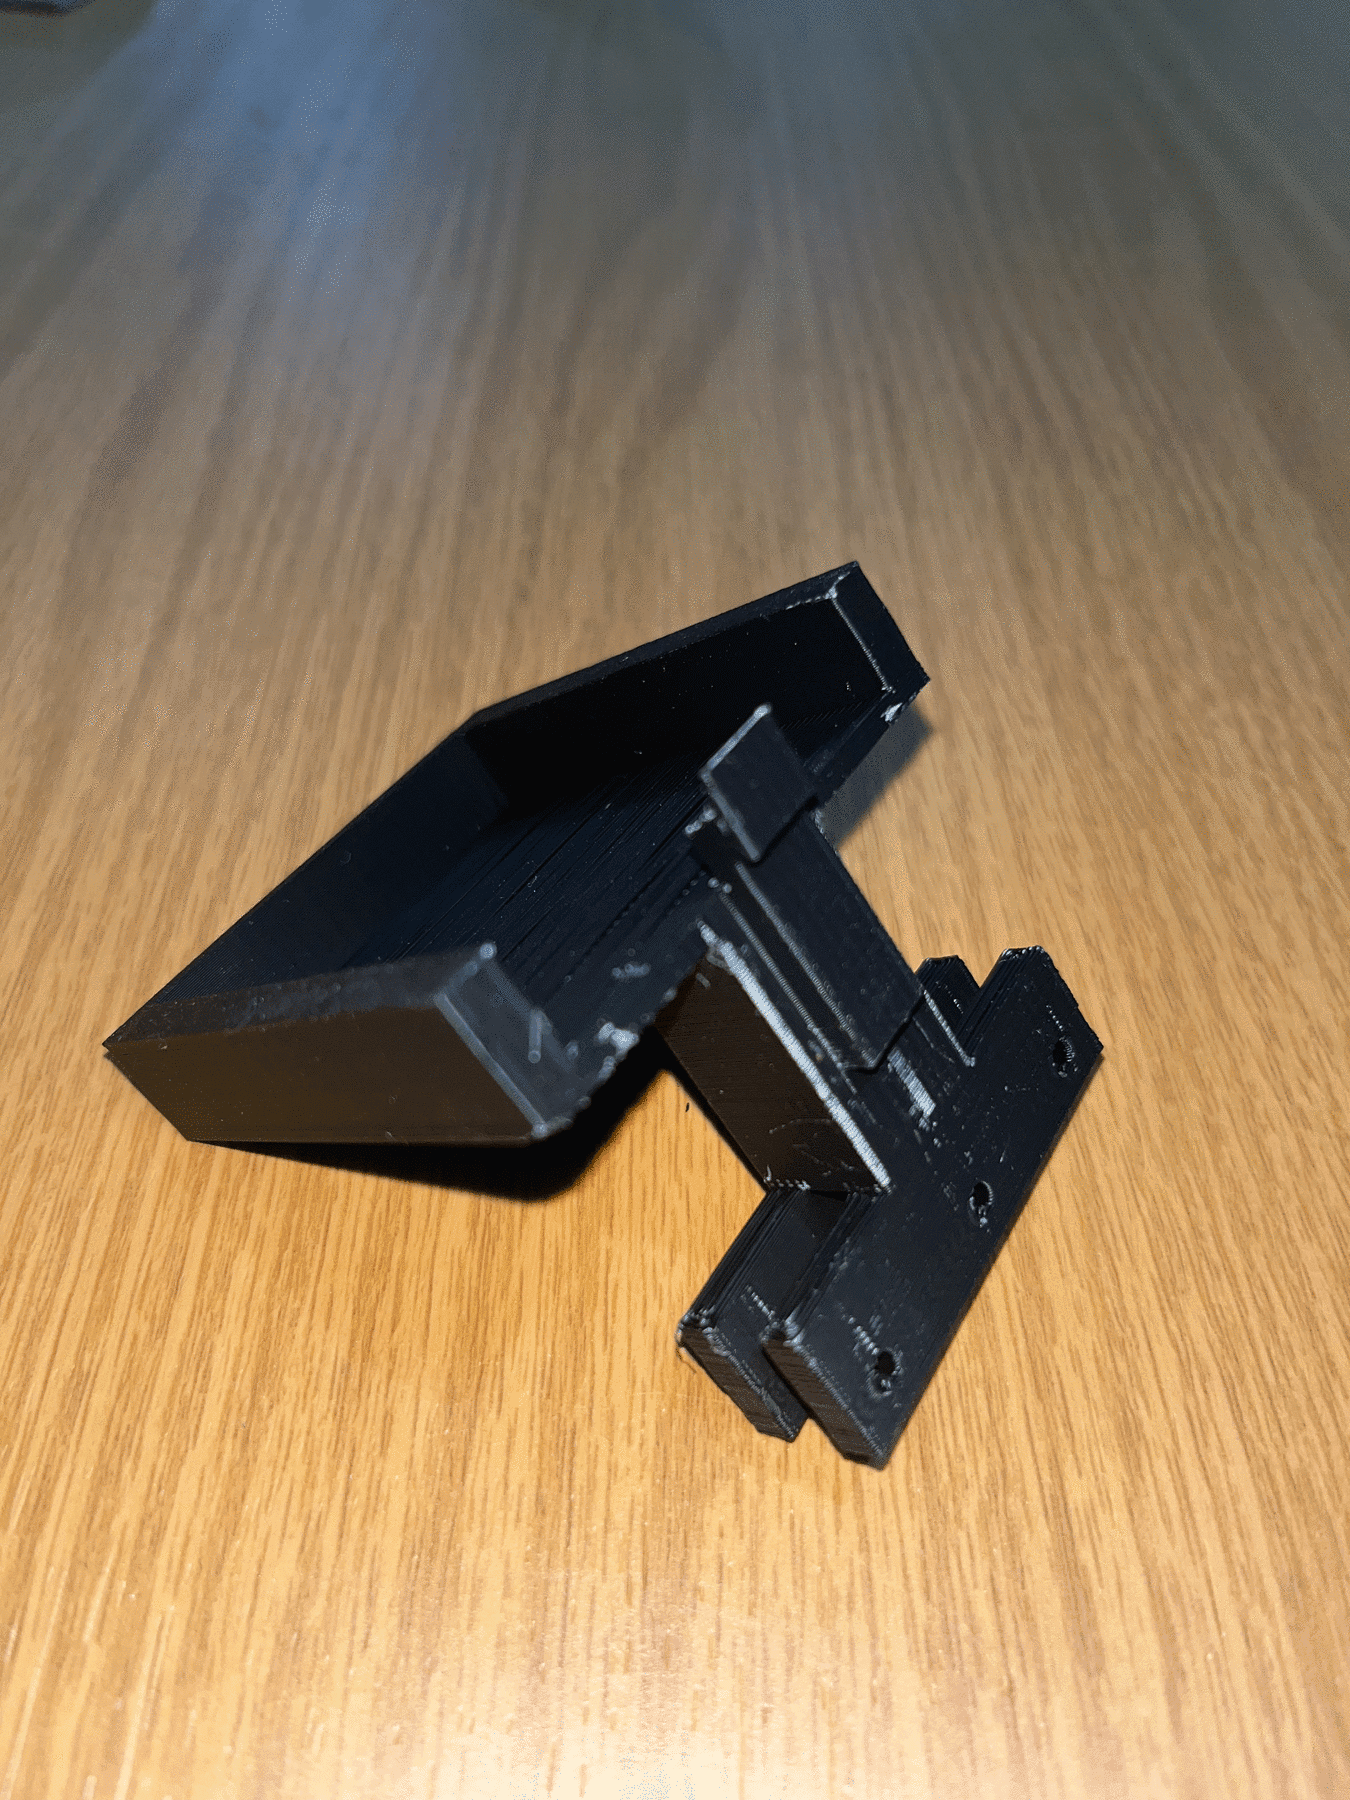
\includegraphics[width=0.7\linewidth]{bab3/casing_kamera_real1}
	\caption{Hasil Pencetakan / Implementasi Fisik Casing Kamera}
	\label{fig:webcam-back-real-1}
\end{figure}

Penyempurnaan pada komponen Casing kamera dilakukan untuk mengatasi masalah kestabilan sudut pandang kamera. Pada desain sebelum revisi, dudukan penyangga bodi Logitech C922 memiliki celah toleransi yang terlalu longgar, sehingga terjadi pergeseran sudut inklinasi akibat getaran frekuensi tinggi dari motor drone saat terbang. Desain baru memperluas area kontak dan memposisikan penahan kamera secara lebih rapat sehingga orientasi kamera tetap stabil sepanjang durasi misi pencarian.

\paragraph{Tutup Kamera}
\begin{figure}[H]
	\centering
	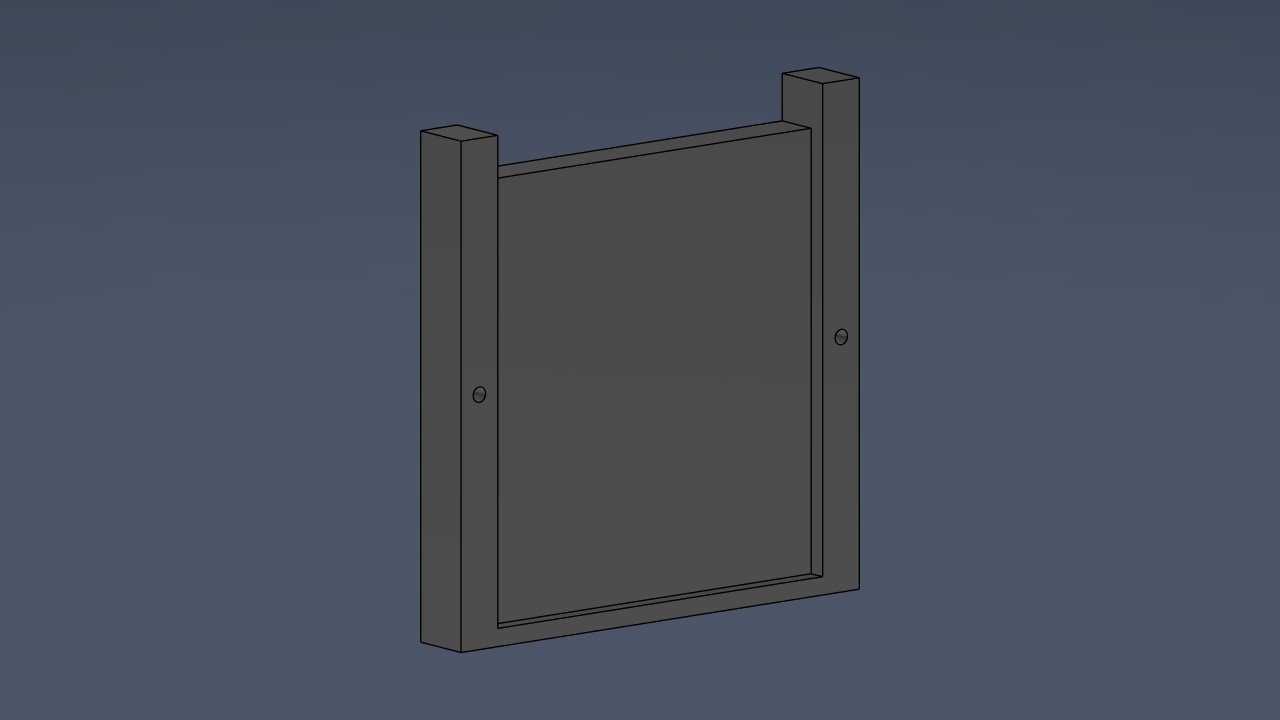
\includegraphics[width=0.7\linewidth]{bab3/tutup_kamera_3d_1}
	\caption{CAD Desain Sebelum Revisi (Tutup Kamera)}
	\label{fig:tutup-kamera-awal-3d-1}
\end{figure}

\begin{figure}[H]
	\centering
	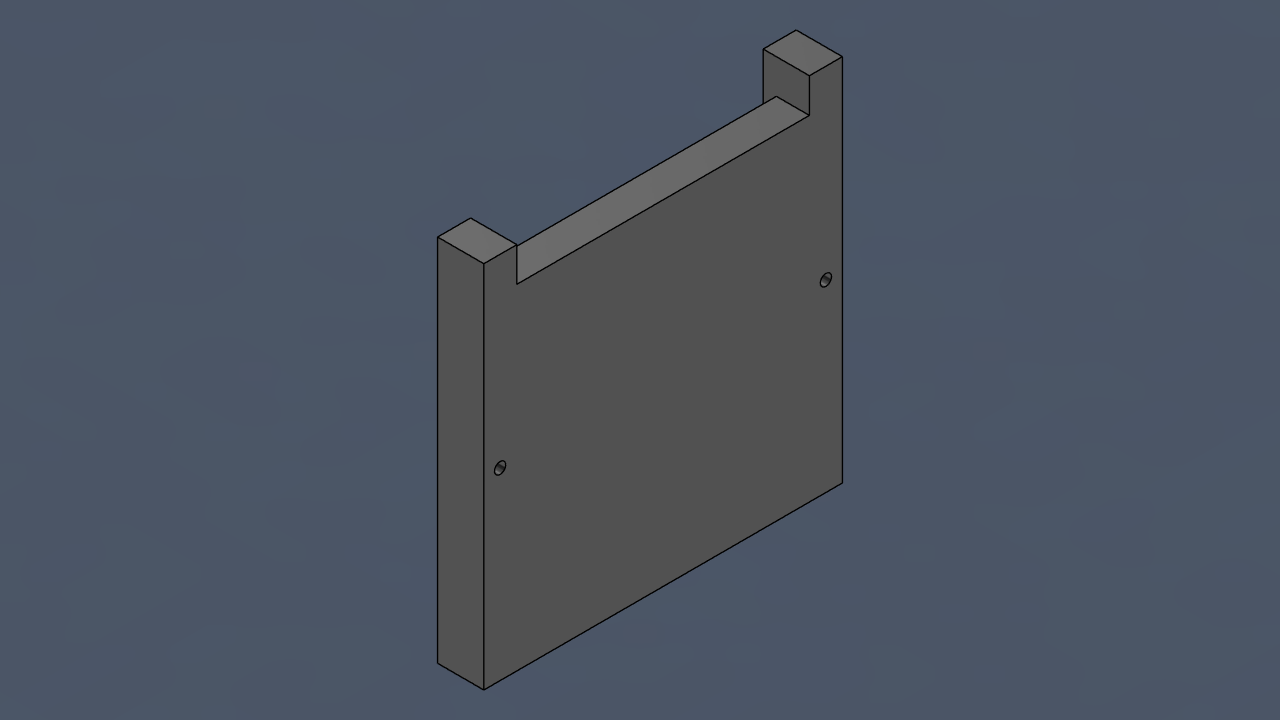
\includegraphics[width=0.7\linewidth]{bab3/tutup_kamera_3d_2}
	\caption{CAD Desain Setelah Revisi (Tutup Kamera)}
	\label{fig:tutup-kamera-awal-3d-2}
\end{figure}

\begin{figure}[H]
	\centering
	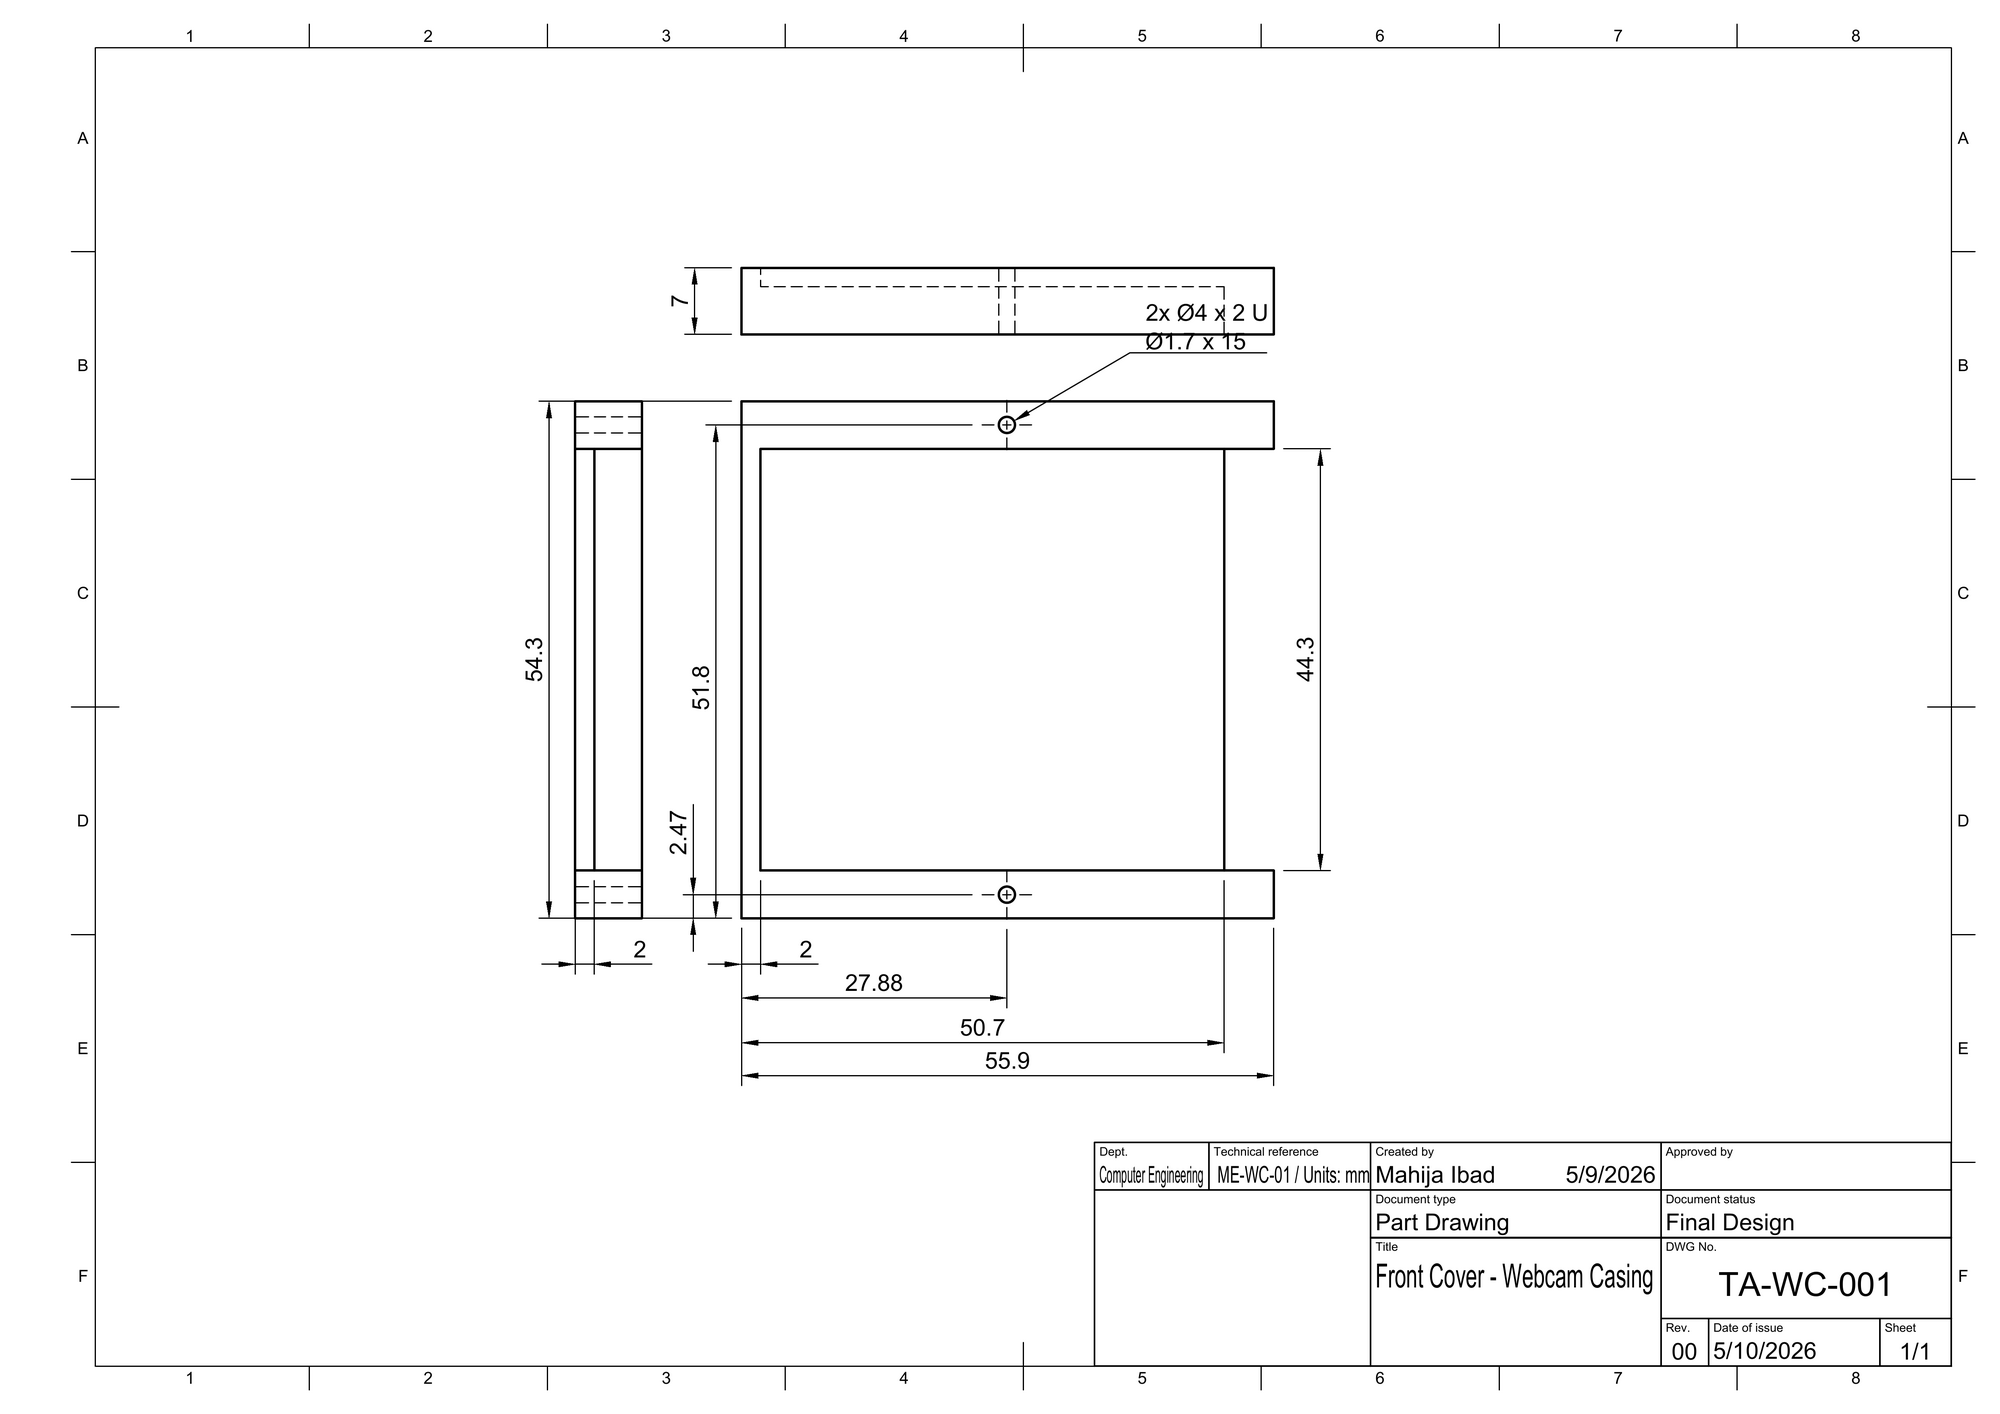
\includegraphics[width=0.7\linewidth]{bab3/tutup_kamera_2d}
	\caption{Gambar Teknik (2D Drawing) Tutup Kamera}
	\label{fig:tutup-kamera-awal-2d}
\end{figure}

\begin{figure}[H]
	\centering
	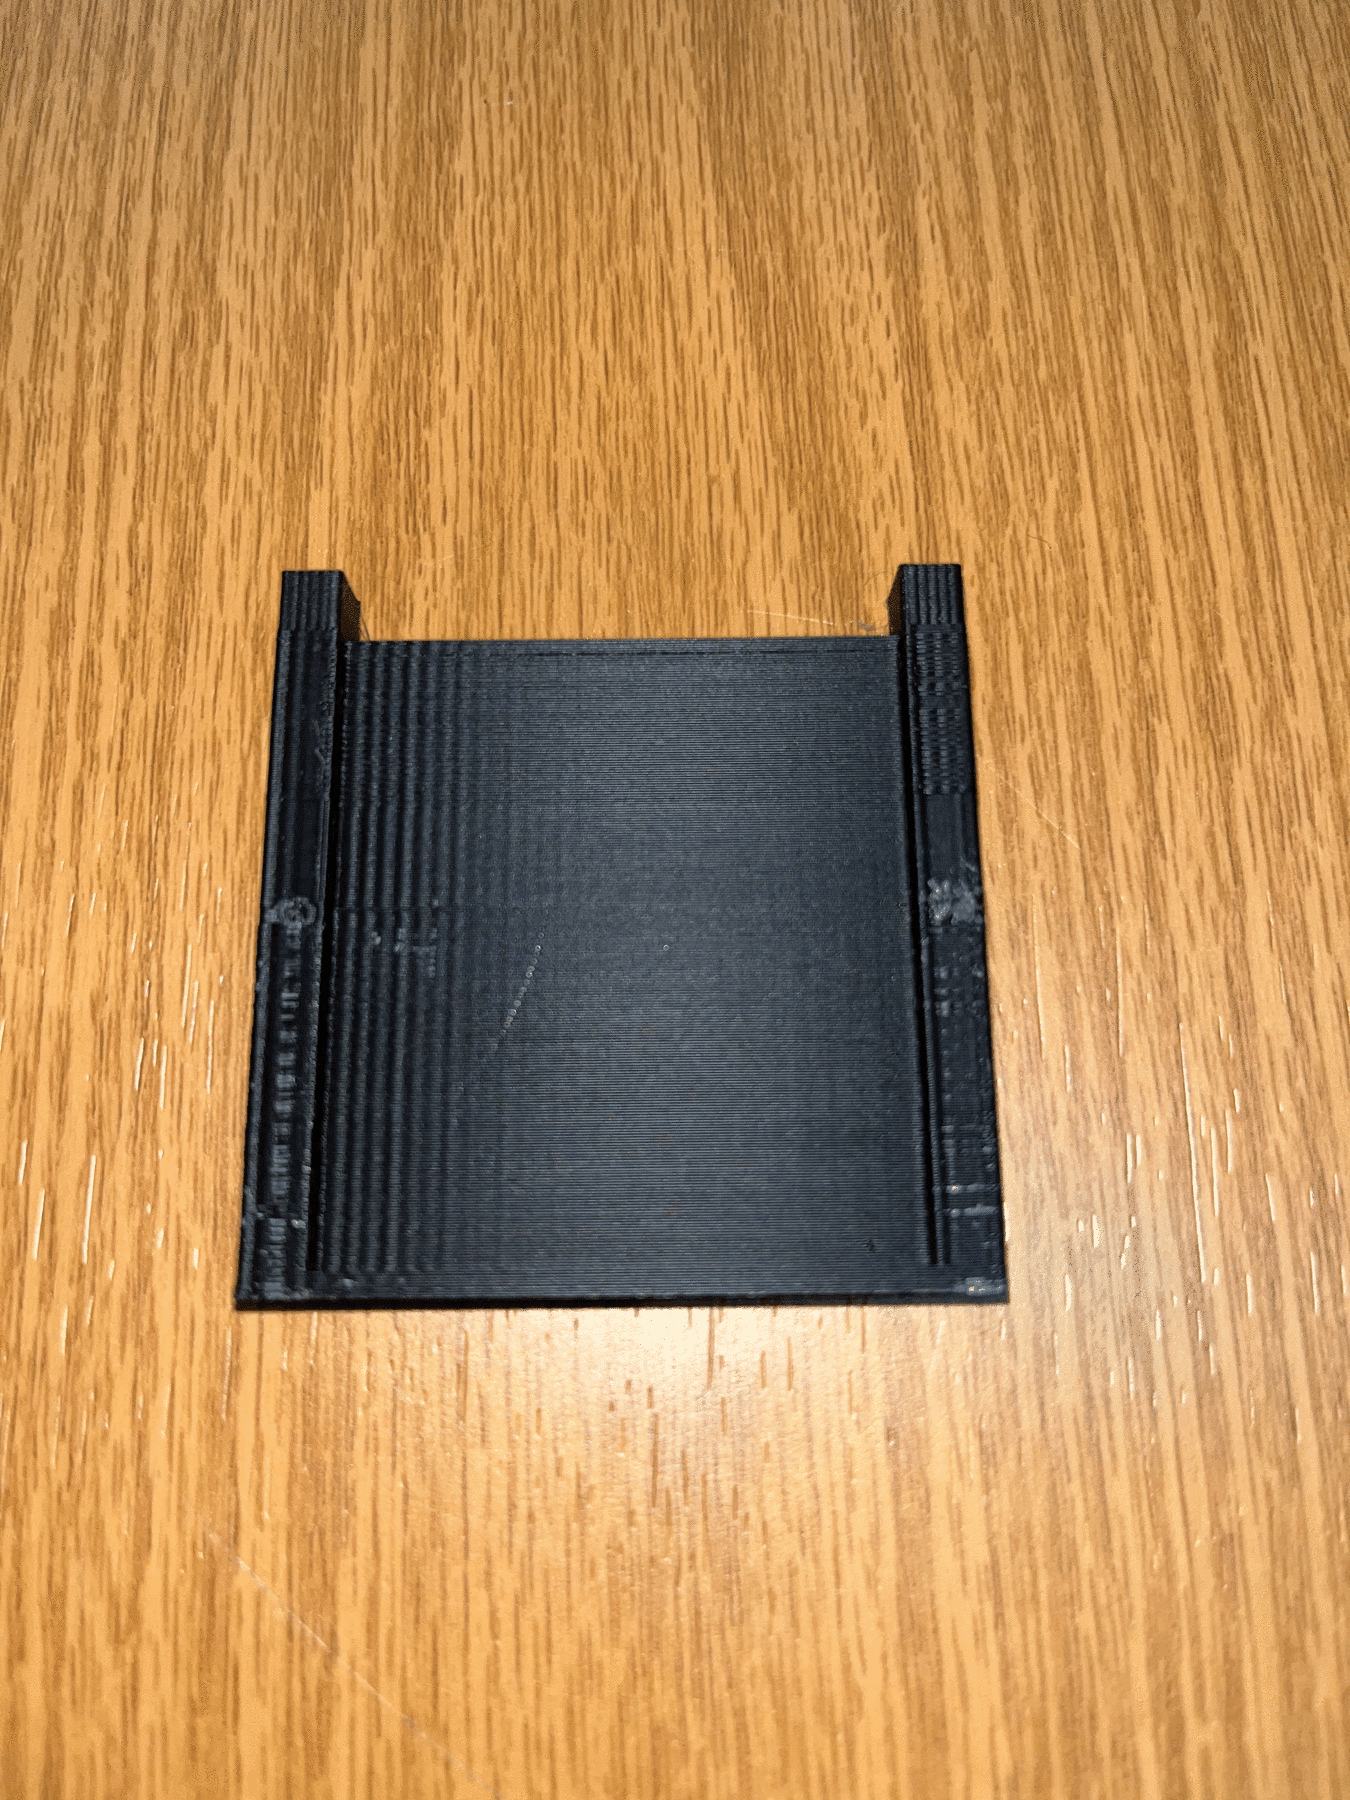
\includegraphics[width=0.7\linewidth]{bab3/tutup_kamera_real1}
	\caption{Hasil Pencetakan / Implementasi Fisik Tutup Kamera}
	\label{fig:webcam-front-real-1}
\end{figure}

Penyempurnaan pada Tutup kamera menyangkut mekanisme penjepitan bodi kamera pada Casing kamera. Desain ulir baut penarik direvisi agar lebih presisi guna menjamin jepitan yang merata pada seluruh sisi bodi webcam, mencegah pergeseran arah pandang kamera saat drone berakselerasi secara mendadak.

\paragraph{Casing Raspberry Pi}
\begin{figure}[H]
	\centering
	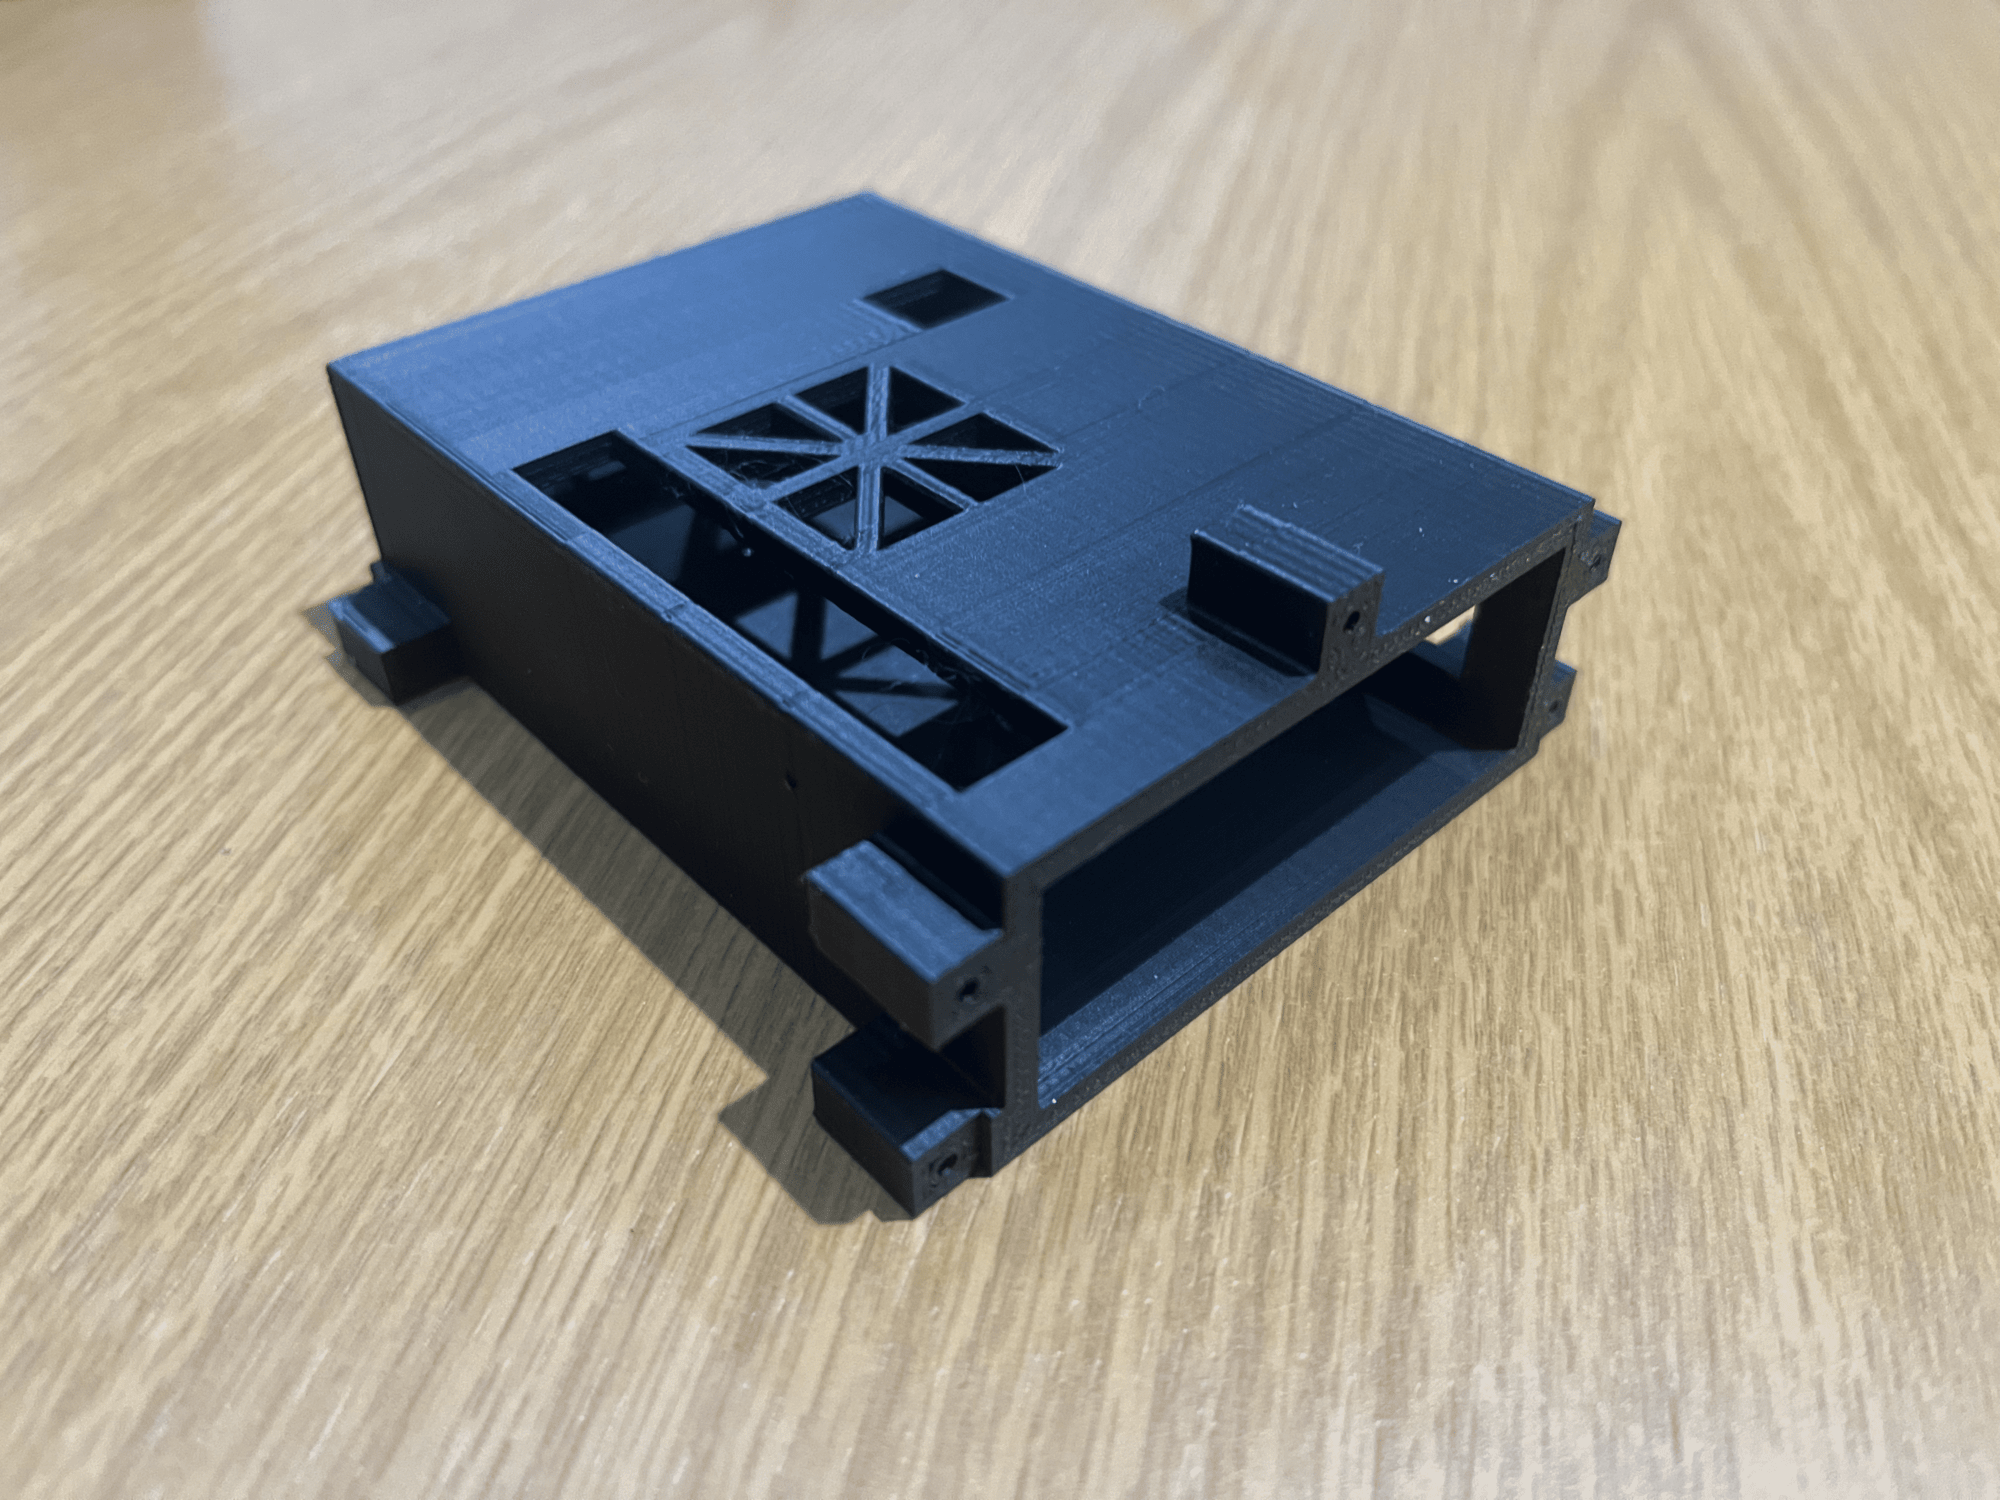
\includegraphics[width=0.7\linewidth]{bab3/casing_raspberry_pi}
	\caption{Casing Raspberry Pi (Desain Final)}
	\label{fig:casing_raspi_baru}
\end{figure}

\begin{figure}[H]
	\centering
	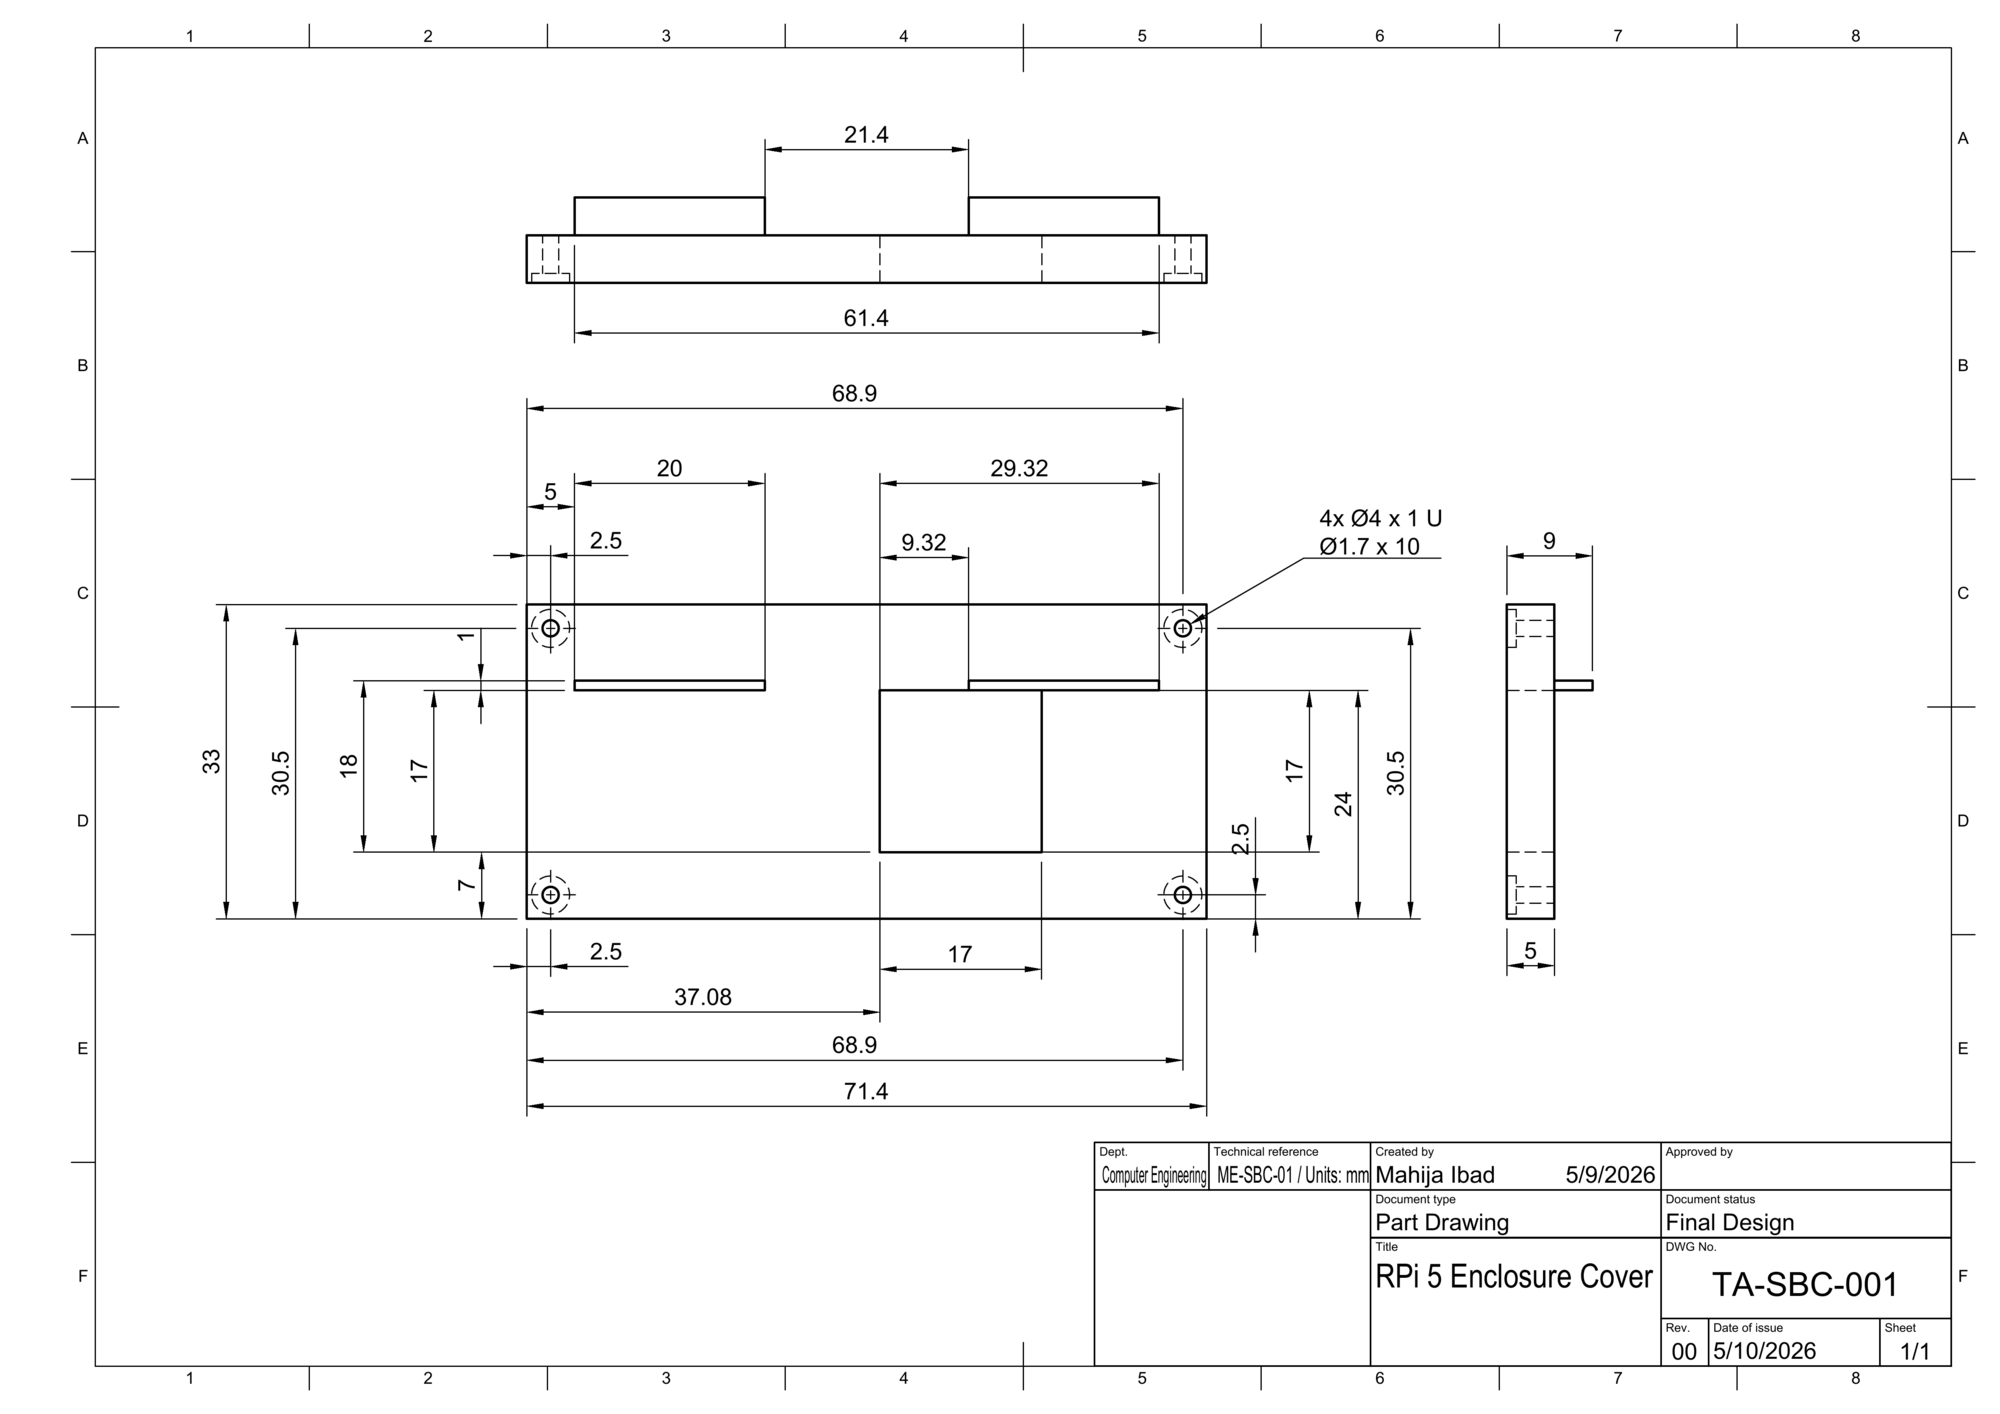
\includegraphics[width=0.7\linewidth]{bab3/casing_raspberry_pi_2d}
	\caption{Gambar Teknik (2D Drawing) Casing Raspberry Pi}
\end{figure}

\begin{figure}[H]
	\centering
	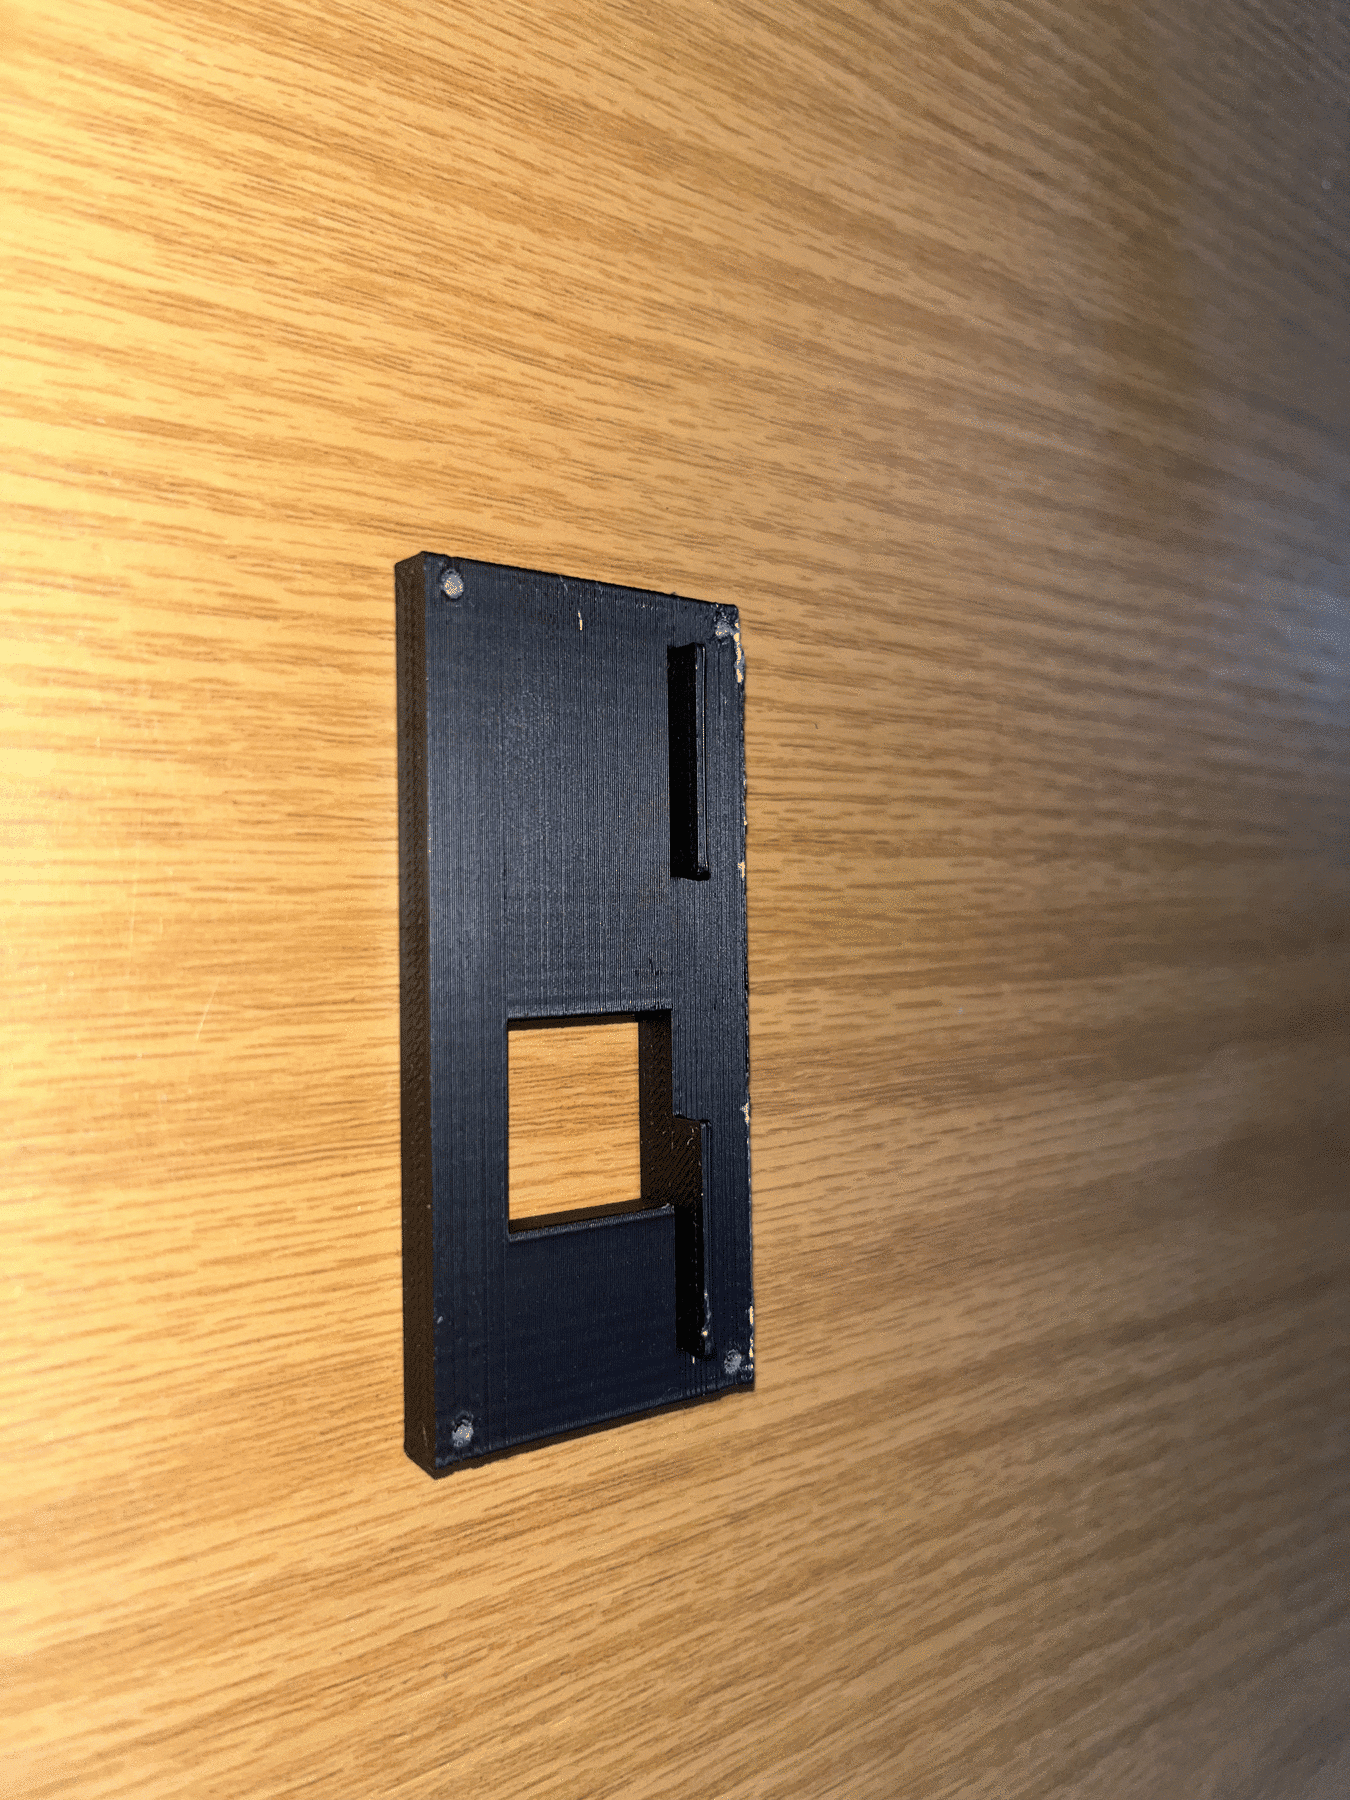
\includegraphics[width=0.7\linewidth]{bab3/casing_raspberry_pi_real1}
	\caption{Hasil Pencetakan / Implementasi Fisik Casing Raspberry Pi}
\end{figure}

Casing Raspberry Pi dirancang khusus untuk melindungi companion computer Raspberry Pi 5. Komponen ini memiliki celah pembuangan panas yang memadai serta lubang baut pengunci presisi untuk memastikan papan sirkuit tetap kokoh berada di posisinya selama penerbangan.

\paragraph{Casing Modem}
\begin{figure}[H]
	\centering
	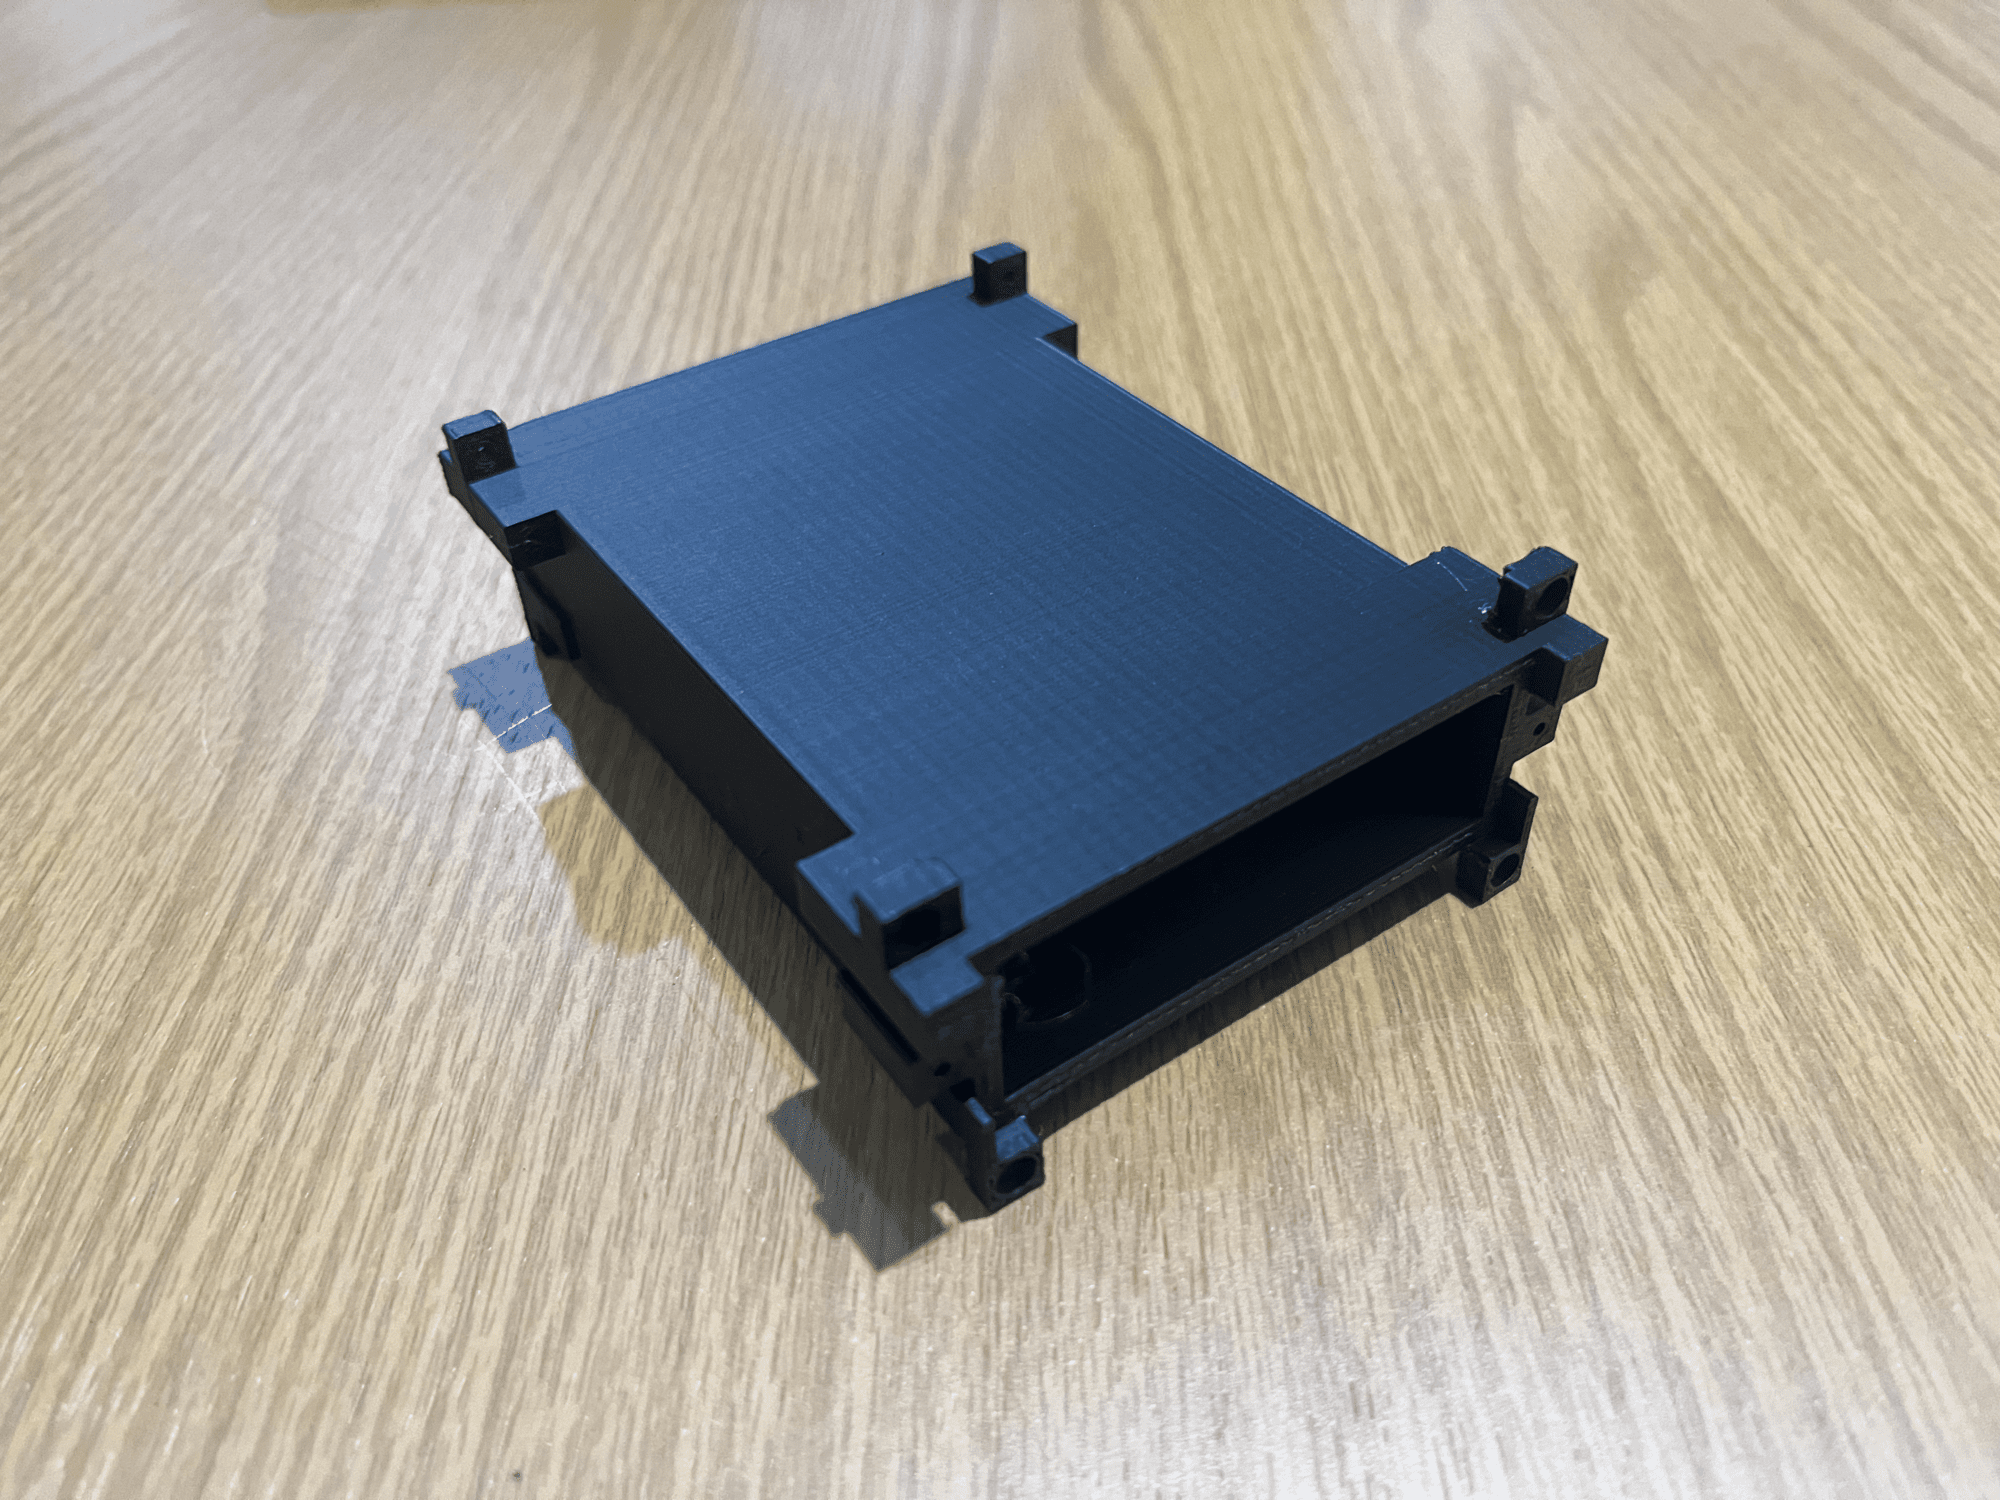
\includegraphics[width=0.7\linewidth]{bab3/casing_modem}
	\caption{Casing modem (Desain Final)}
	\label{fig:casing_modem_baru}
\end{figure}

\begin{figure}[H]
	\centering
	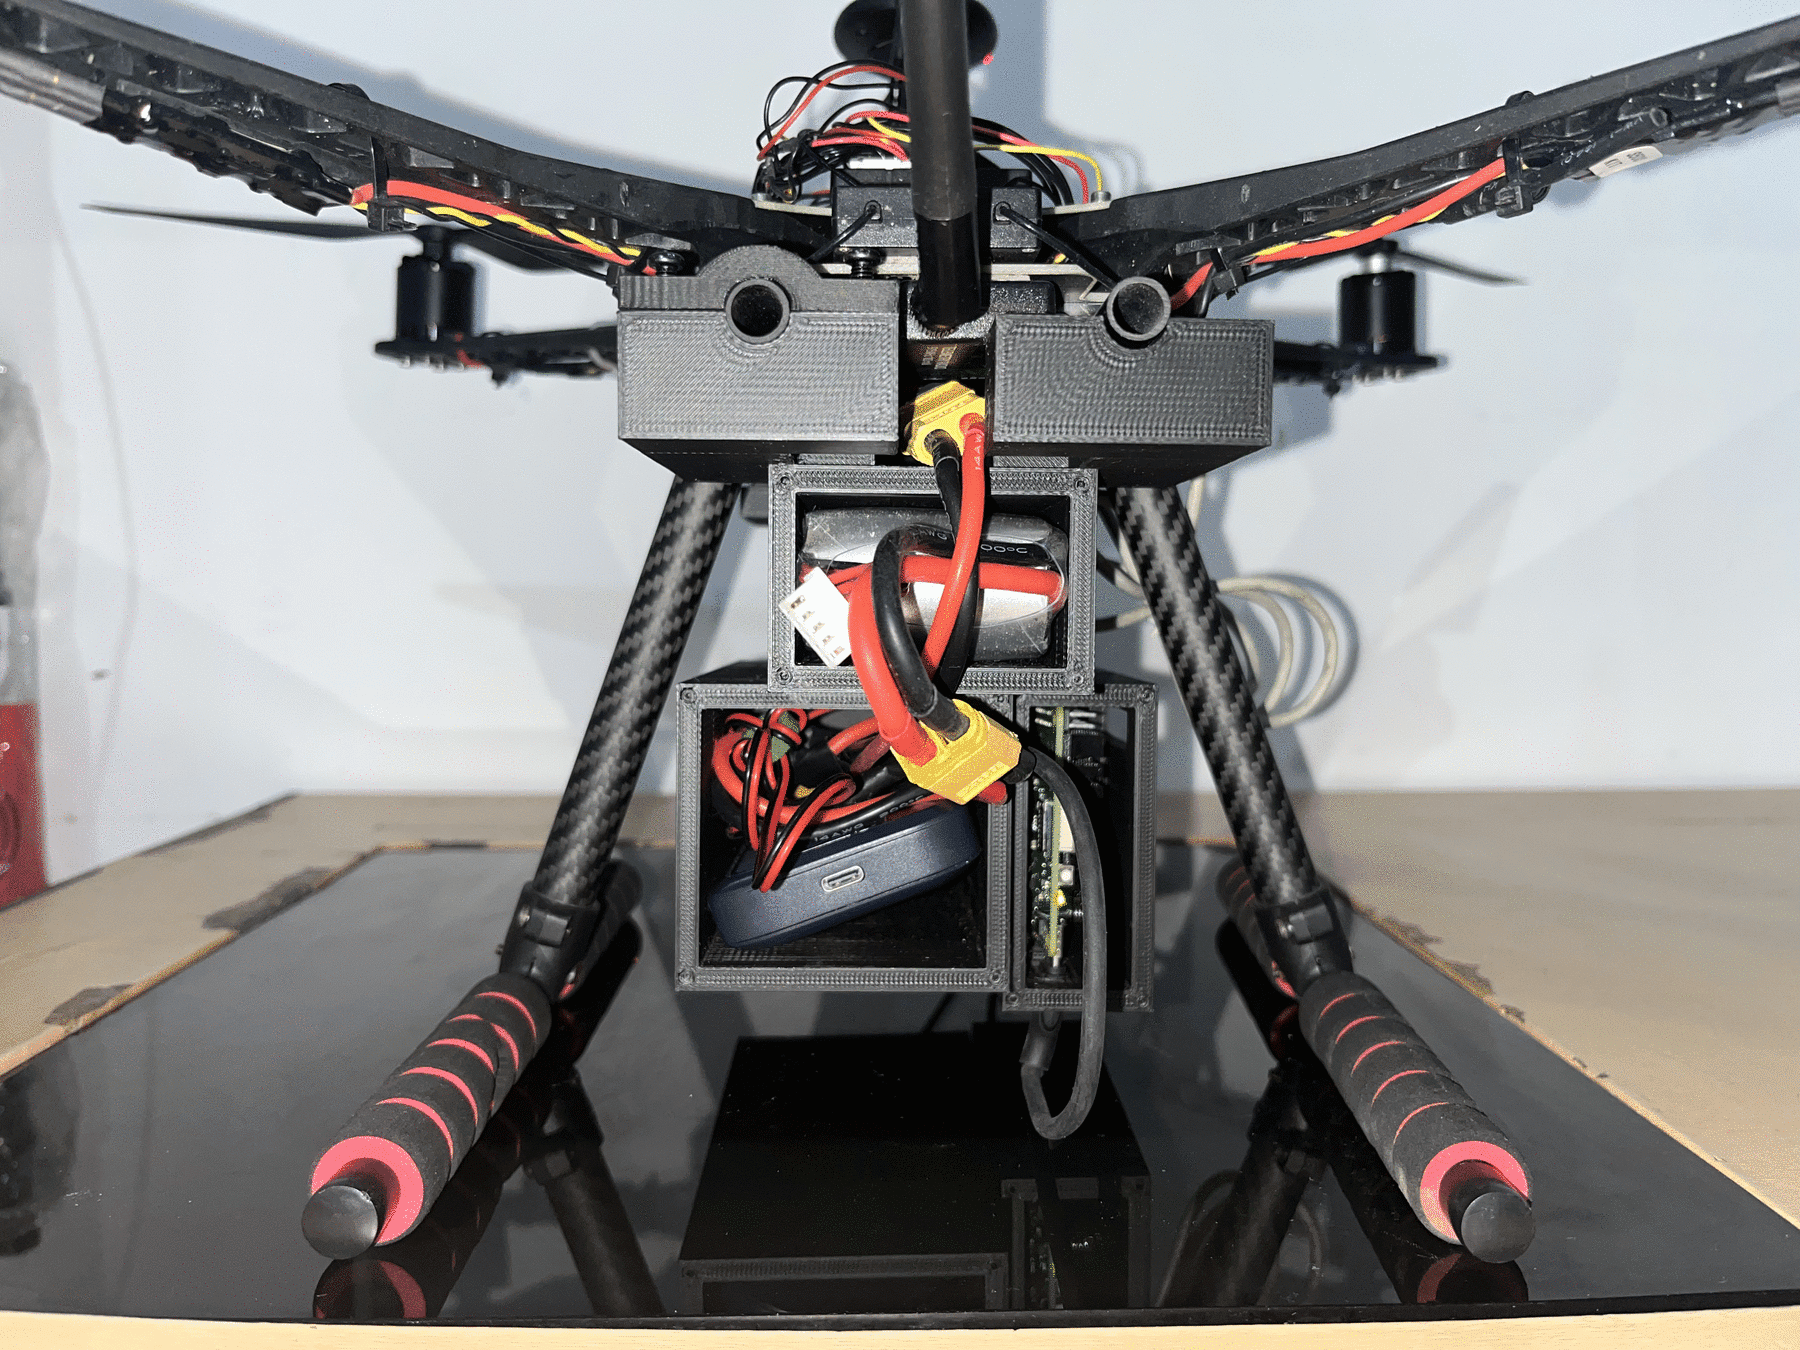
\includegraphics[width=0.7\linewidth]{bab3/modem_mifi_4g_casing}
	\caption{Penempatan Modem pada Casing}
\end{figure}

Casing modem menggantikan peran casing power supply terpisah pada desain awal. Komponen ini dirancang untuk menampung unit modem MiFi secara kompak untuk mendukung komunikasi data otonom dan pengiriman telemetri video langsung kepada operator secara stabil.


\subsection{Desain Software}
Desain perangkat lunak pada sistem drone otonom ini dirancang untuk menangani tingkat kompleksitas yang tinggi, mencakup navigasi otomatis, deteksi manusia secara \textit{real-time}, pengolahan data telemetri, dan pemantauan sistem. Sistem ini mengimplementasikan arsitektur \textit{multi-thread} dan \textit{asynchronous} terdistribusi untuk memastikan bahwa pemrosesan berat seperti inferensi kecerdasan buatan tidak memblokir atau mengganggu \textit{loop} kontrol penerbangan kritis.

Secara keseluruhan, arsitektur perangkat lunak dibagi menjadi beberapa subsistem utama: server \textit{backend} (Flask + SocketIO), \textit{pipeline} pemrosesan video (GStreamer), modul deteksi manusia (YOLO), mesin \textit{state machine} otonom (MAVSDK), serta antarmuka \textit{frontend} berbasis React.

\subsubsection{Arsitektur Backend dan Threading}
\textit{Backend} sistem bertindak sebagai pusat orkestrasi yang mengelola seluruh modul. Untuk mencegah \textit{bottleneck} komputasi, arsitektur ini memisahkan proses ke dalam beberapa \textit{thread} independen:
\begin{itemize}
	\item Main Thread (Flask + SocketIO): Bertugas menangani \textit{REST API} dan komunikasi \textit{WebSocket} dengan antarmuka pengguna (\textit{frontend}).
	\item MAVSDK Thread: Berjalan sebagai \textit{daemon thread} yang didedikasikan untuk \textit{asyncio event loop}. \textit{Thread} ini mengelola komunikasi \textit{telemetry} dari \textit{flight controller} dan menjalankan algoritma otonom pada frekuensi tinggi (20Hz) tanpa interupsi.
	\item GStreamer Thread: Menggunakan \textit{GLib MainLoop} untuk menangani akuisisi \textit{frame} dari kamera secara perangkat keras tingkat rendah (\textit{low-level}).
	\item YOLO Consumer Thread: \textit{Daemon thread} terpisah yang melakukan inferensi jaringan saraf tiruan secara \textit{blocking}. Pemisahan ini krusial agar latensi komputasi YOLO tidak menghentikan pengiriman sinyal kontrol ke drone.
\end{itemize}

\subsubsection{Pipeline Video dan GStreamer}
\begin{figure}[H]
	\centering
	\includegraphics[width=0.4\linewidth]{bab3/flow3-31.pdf}
	\caption{Blok Diagram Pipeline Video}
	\label{fig:blokpipeline}
\end{figure}
Subsistem akuisisi video dirancang menggunakan GStreamer untuk mendistribusikan aliran data visual dengan efisiensi tinggi melalui mekanisme \textit{tee pipeline}. Alur pemrosesan dimulai dari kamera USB (\texttt{/dev/video*}) yang ditangkap oleh \texttt{v4l2src}. Aliran ini kemudian dicabangkan (\textit{branching}):
\begin{itemize}
	\item Branch Streaming: Menggunakan perangkat lunak \textit{encoder} H.264 (atau \textit{hardware encoder} \texttt{v4l2h264enc}) untuk mentransmisikan video latensi rendah via protokol UDP pada \textit{port} 5600, yang ditujukan untuk GCS (\textit{Ground Control Station}) eksternal. Cabang ini juga menyediakan \textit{fallback} berupa aliran \textit{Motion JPEG} (MJPEG) pada \textit{endpoint} \textit{REST API} untuk pemantauan antarmuka dasbor berbasis web. Guna mereduksi beban komputasi CPU, aktivitas \textit{storage I/O}, serta memperpanjang usia pakai kartu memori (\textit{SD-card}) pada Raspberry Pi 5, seluruh sistem perekaman video di atas wahana (\textit{onboard video recording}) beserta rute-rute penyimpanan berkas video telah sepenuhnya ditiadakan dari sistem \textit{backend} dan dasbor \textit{frontend}, menjadikan media penyimpanan terfokus secara eksklusif pada hasil dokumentasi foto korban.
	\item Branch YOLO: \textit{Frame} diarahkan ke \texttt{appsink} yang kemudian memasukkan citra ke dalam \textit{frame queue} dengan mekanisme penjatuhan \textit{frame} lama (\textit{leaky queue}) guna memastikan sistem deteksi selalu mendapatkan citra paling baru (\textit{latest frame}).
\end{itemize}

\subsubsection{Arsitektur Deteksi YOLO}
\begin{figure}[H]
	\centering
	\includegraphics[width=0.6\linewidth]{bab3/flow3-32.pdf}
	\caption{Flowchart Deteksi \& Target Lock}
	\label{fig:flowyolo}
\end{figure}

Modul deteksi berfungsi menerjemahkan data piksel mentah menjadi koordinat target spasial yang akan digunakan oleh sistem kendali terbang. Berdasarkan hasil analisis dan tahapan optimasi, sistem ini menggunakan model YOLOv8n standar yang telah melalui proses \textit{fine-tuning} khusus untuk deteksi kelas tunggal manusia (\textit{person-only}) menggunakan dataset COCO yang difilter dengan total kotak pembatas anotasi sebanyak 244.799 instans target. Model final PyTorch (\texttt{best.pt}) berukuran 6,0 MB tersebut kemudian diekspor ke dalam format ONNX dengan resolusi input sebesar 320x320 piksel (\texttt{320n.onnx}) untuk diimplementasikan pada perangkat \textit{edge} \textit{companion computer} Raspberry Pi 5.

Pemilihan resolusi input 320x320 piksel dengan format ONNX didasarkan pada titik temu (\textit{trade-off}) paling optimal antara performa komputasi dan akurasi deteksi. Strategi pemangkasan ruang prediksi menjadi kelas tunggal ini mampu mendongkrak nilai mAP@50 secara signifikan hingga mencapai 0,757 (meningkat sekitar 13\% dibandingkan model \textit{baseline} multi-kelas COCO) serta meraih tingkat \textit{Precision} sebesar 80,9\%. Reduksi ukuran input dan pemfokusan kelas ini sangat krusial untuk meminimalkan latensi pemrosesan (\textit{inference time}), sehingga sirkuit asinkron \textit{YOLO Consumer} tetap mampu memasok data secara konstan agar selaras dengan frekuensi \textit{loop} kontrol otonom utama yang bekerja pada 20 Hz.

Alur logika pemrosesan dirancang mengalir secara asinkron, di mana komponen \texttt{YOLO Consumer} mengambil citra dari \textit{frame queue} dan memprosesnya menggunakan model tersebut melalui \textit{ONNX Runtime}. Untuk menjaga stabilitas penentuan target di lingkungan dinamis dan mencegah transisi yang tidak stabil (\textit{target ping-pong}), sistem mengimplementasikan algoritma pemeringkatan (\textit{scoring}) dan penguncian target (\textit{target lock}) \cite{BarShalom2001Tracking}. Kandidat target dievaluasi berdasarkan kombinasi pembobotan linear sebagai berikut:

\begin{itemize}
	\item Luas area kotak pembatas (\textit{bounding box}) sebesar 45\%, sebagai indikator kedekatan jarak fisik target terhadap sensor kamera.
	\item Nilai tingkat keyakinan (\textit{confidence score}) dari model sebesar 25\%, sebagai validasi kepastian objek.
	\item Kedekatan posisi koordinat target terhadap titik tengah (\textit{center of frame}) sebesar 20\%, untuk menjaga keterpusatan orientasi drone.
	\item Konsistensi pelacakan spasial antar-frame (\textit{tracking history}) sebesar 10\%, untuk memvalidasi kontinuitas pergerakan target.
\end{itemize}

Sistem dirancang untuk menahan fokus (\textit{lock}) pada satu target utama terpilih dan tidak akan berpindah ke objek manusia lain kecuali objek baru memiliki skor minimal 35\% lebih tinggi. Setelah target dipastikan, titik koordinat lokasinya secara asinkron didistribusikan ke dalam antrean sistem (\textit{detection queue}) agar dapat diproses oleh pengendali otonom.

\subsubsection{State Machine Sistem Otonom}
\begin{figure}[H]
	\centering
	\includegraphics[width=0.8\linewidth]{bab3/flow3-33.pdf}
	\caption{State Machine Diagram Sistem Otonom Drone}
	\label{fig:statemachine}
\end{figure}
Inti dari logika pencarian dan penyelamatan direpresentasikan melalui \textit{state machine} hierarkis yang dikendalikan oleh \textit{Autonomy Controller}. Sistem ini mendukung dua mode operasional:
\begin{enumerate}
	\item Standard Mode: Mode dasar saat kendali \textit{OFFBOARD} aktif, terdiri dari \textit{state} \texttt{SEARCHING} (berputar secara statis mencari target), \texttt{TRACKING} (menjaga posisi relatif terhadap target terdeteksi), dan \texttt{EMERGENCY}.
	\item Scout Mission Mode: Siklus otonom terstruktur untuk operasi SAR, mencakup:
	\begin{itemize}
		\item \texttt{SCOUT\_SCAN}: Drone melakukan rotasi secara perlahan (\textit{yaw rate} 30 deg/s) untuk menyapu dan memperluas area observasi.
		\item \texttt{SCOUT\_APPROACH}: Saat target manusia dikunci, drone bermanuver mendekat. Kecepatan pendekatan dikomputasi dan dihaluskan melalui filter \textit{Exponential Moving Average} (EMA).
		\item \texttt{SCOUT\_DOCUMENT}: Drone menahan posisinya di udara (\textit{hold setpoint}) di dekat korban, memvalidasi radius eksklusi sejauh 3,0 meter menggunakan komputasi jarak \textit{Haversine} untuk memastikan bahwa target tidak berada di koordinat yang sudah dikunjungi sebelumnya, lalu mengambil dokumentasi (\textit{screenshot}) visual-spasial.
		\item \texttt{SCOUT\_DISPLACING}: Begitu dokumentasi selesai, drone melakukan pergeseran posisi secara lateral (sejauh 2 meter ke kanan) guna perluasan cakupan area secara kontinu dan pencarian korban yang persisten. Drone kemudian kembali memasuki \textit{state} \texttt{SCOUT\_SCAN} untuk melanjutkan misi secara berkelanjutan. Prosedur kembali ke titik asal (\texttt{RETURN\_HOME}) bukan bagian dari siklus pencarian normal; kepulangan akibat baterai kritis ditangani terpisah oleh fitur RTL bawaan PX4.
	\end{itemize}
\end{enumerate}

\subsubsection{Sistem Telemetri dan Komunikasi Realtime (SocketIO)}
Sistem telemetri dirancang untuk memfasilitasi pertukaran data kecepatan tinggi antara \textit{flight controller} dan antarmuka pengguna (\textit{frontend}). Modul \textit{MAVSDK Listener} membuka 8 aliran data (\textit{stream}) asinkron untuk memantau posisi, kapasitas baterai, mode penerbangan, orientasi, dan konstelasi GPS secara simultan.

Keseluruhan informasi tersebut diperbarui secara terpusat pada kamus \textit{state} internal. Sebuah \textit{loop} penyiaran (\textit{broadcast loop}) berjalan membelah sistem secara periodik pada frekuensi 5Hz, mengambil cuplikan (\textit{snapshot}) matriks data telemetri terkini, dan memancarkannya (\textit{emit}) melalui \textit{SocketIO} di bawah \textit{event} \texttt{drone:status}. Selain disiarkan, matriks telemetri ini juga direkam secara persisten ke dalam sistem \textit{rotating log} internal dengan pembatasan laju (\textit{rate limit}) 5Hz untuk memfasilitasi kebutuhan analisis misi pasca-penerbangan tanpa menghambat performa inti pemrosesan. Pada ujung antarmuka (React), pembaruan data yang sangat responsif ini ditangkap dan merender dasbor operator secara instan.

\subsubsection{Sistem Watchdog dan Prosedur Keselamatan}
Sebagai sistem udara tanpa awak yang didesain untuk ranah pencarian korban di area bencana, integritas dan keamanan misi ditangani secara ketat lewat \textit{watchdog} perangkat lunak dan arsitektur keselamatan (\textit{safety procedure}):
\begin{itemize}
	\item OFFBOARD Keepalive: Mengingat batasan keamanan internal \textit{firmware} PX4, sistem secara konstan menembakkan setpoint instruksi kendali bernilai netral (\textit{keepalive}) sebanyak 20 kali per detik bahkan saat drone masih di darat. Ini adalah mitigasi agar PX4 mengizinkan perpindahan \textit{mode} penerbangan ke \textit{OFFBOARD} kapan pun pilot pada kendali radio menginginkannya.
	\item Connection Watchdog: Mengawasi kontinuitas koneksi dari MAVSDK. Apabila putus dalam durasi tertentu, sistem seketika memicu perintah berhenti darurat (\textit{emergency stop}).
	\item Battery RTL Mechanism: Telemetri baterai dipantau secara kontinu. Apabila tingkat kapasitas baterai menyentuh ambang batas kritis sebesar $< 15\%$, sistem secara otomatis membatalkan seluruh tugas navigasi dan memicu fase pengamanan berupa pendakian paksa vertikal (\textit{pre-RTL safety climb}) selama 3,0 detik ke atas pada kecepatan $vz = -0,8$ m/s guna memitigasi efek penyimpangan barometer (\textit{barometric drift}). Setelah fase pendakian keselamatan selesai, drone mengirimkan perintah mode \textit{Return to Launch} (RTL) bawaan PX4 secara aman untuk menghentikan misi dan pulang ke titik asal lepas landas.

	Mekanisme \textit{Battery Return-to-Launch} (RTL) yang diimplementasikan pada penelitian ini murni merupakan mekanisme keselamatan pada perangkat lunak otonom di \textit{companion computer} Raspberry Pi 5 dan sama sekali tidak menggunakan estimasi energi penerbangan. Sistem tidak menghitung kebutuhan energi berdasarkan jarak spasial menuju titik asal (\textit{home position}), tidak melakukan prediksi sisa waktu terbang (\textit{remaining flight time}), serta tidak mengestimasi konsumsi daya motor propulsi. Keputusan aktivasi Battery RTL menggunakan pendekatan \textit{fixed threshold} sebesar 15\% berdasarkan persentase baterai yang diterima melalui telemetri MAVSDK.

	Nilai ambang batas sebesar 15\% ditetapkan sebagai parameter keselamatan operasional sistem. Nilai tersebut dipilih secara empiris berdasarkan konfigurasi pengujian yang digunakan pada penelitian ini. Threshold digunakan untuk menjamin tersedianya energi yang memadai selama:
	\begin{itemize}
		\item penghentian misi aktif,
		\item pelaksanaan \textit{Pre-RTL Safety Climb},
		\item transisi mode penerbangan,
		\item dan proses \textit{Return-to-Launch}.
	\end{itemize}
	Urutan kerja operasional dari mekanisme keselamatan \textit{Battery RTL} ini berjalan secara sekuensial. Awalnya, \textit{Battery Sensor} mengukur status fisik daya baterai, lalu mengirimkannya ke \textit{PX4 Battery Estimator} untuk diestimasi persentasenya. Data persentase baterai ini ditransmisikan melalui \textit{MAVSDK Telemetry} ke \textit{companion computer} Raspberry Pi 5. Raspberry Pi 5 memonitor nilai persentase baterai ini secara terus-menerus. Ketika kapasitas baterai berada di atas batas kritis ($> 15\%$), misi penerbangan otonom tetap dilanjutkan (\textit{Continue Mission}). Namun, jika nilai persentase baterai mencapai atau kurang dari ambang batas ($\le 15\%$), Raspberry Pi 5 akan segera mengambil keputusan untuk menghentikan misi secara aktif (\textit{Abort Mission}). Selanjutnya, Raspberry Pi 5 memicu fase pengamanan \textit{Pre-RTL Safety Climb} dengan melakukan pendakian vertikal selama 3 detik pada kecepatan $vz = -0,8$ m/s. Setelah fase pendakian keselamatan selesai, Raspberry Pi 5 memanggil fungsi \texttt{return\_to\_launch()} secara terprogram melalui perintah aksi MAVSDK (\textit{MAVSDK Action}), sehingga autopilot PX4 kemudian mengeksekusi prosedur kepulangan otomatis (\textit{PX4 RTL}).
	\begin{figure}[H]
		\centering
		\includegraphics[width=0.65\linewidth]{bab3/battery_rtl_flowchart.pdf}
		\caption{Mekanisme Battery RTL Berbasis Fixed Threshold}
		\label{fig:battery_rtl_flowchart}
	\end{figure}

	Gambar~\ref{fig:battery_rtl_flowchart} mendeskripsikan diagram alir dari mekanisme pengamanan baterai otonom. Berdasarkan skema tersebut, dapat diperjelas kembali bahwa \textit{companion computer} Raspberry Pi 5 tidak menghitung kebutuhan energi penerbangan, konsumsi daya motor, \textit{endurance} baterai, \textit{remaining flight time}, maupun jarak spasial menuju \textit{home position}. Raspberry Pi 5 hanya memonitor nilai persentase baterai (\textit{battery percentage}) yang diperoleh dari PX4 melalui telemetri MAVSDK sebagai pemicu logika keselamatan. Ketika persentase baterai mencapai atau kurang dari 15\%, sistem otonom di Raspberry Pi 5 membatalkan misi aktif, melakukan manuver \textit{Pre-RTL Safety Climb}, dan kemudian memanggil fungsi \texttt{return\_to\_launch()} melalui MAVSDK untuk memicu prosedur pulang otomatis.
	\item Target Timeout Mitigation: Ketika berada dalam mode pengejaran target (\texttt{SCOUT\_APPROACH}), bila subjek hilang dari pantauan kamera melampaui 2 detik, atau jika target tak kunjung tergapai melebihi 20 detik, navigasi \textit{approach} dibatalkan dan digugurkan kembali ke awal fase \texttt{SCOUT\_SCAN}.
	\item OFFBOARD Exit Handling: Sistem pemantau MAVSDK secara kontinu mengawasi transisi mode penerbangan. Apabila pilot mengambil alih kendali manual menggunakan \textit{remote controller} sehingga drone keluar dari mode \textit{OFFBOARD}, sistem perangkat lunak secara asinkron akan langsung menggugurkan (\textit{halt}) seluruh siklus misi otonom dengan aman untuk mencegah benturan komando navigasi.
\end{itemize}

\subsection{Desain Arsitektur Sistem}
Desain arsitektur sistem ini menguraikan struktur integrasi logis antara komponen perangkat keras fisik dengan jaringan perangkat lunak otonom pada drone. Perancangan ini dibagi menjadi beberapa lapisan subsistem modular yang saling terhubung secara asinkron untuk mengakomodasi perbedaan kecepatan pemrosesan data (multi-rate system). Bagian ini akan membahas mengenai topologi sinkronisasi arsitektur keseluruhan, pemisahan alur data end-to-end antara jalur kendali terbang dan jalur pemantauan, serta pembagian peran spesifik dari subsistem penerbangan, subsistem komputasi, hingga antarmuka monitoring operator.
\subsubsection{Arsitektur Sistem Keseluruhan dan Sinkronisasi}
\begin{figure}[H]
	\centering
	\includegraphics[width=0.8\linewidth]{bab3/flow3-34.pdf}
	\caption{Blok Diagram Keseluruhan Arsitektur Sistem}
	\label{fig:blokfullarsitektur}
\end{figure}
Arsitektur sistem keseluruhan merepresentasikan integrasi antara subsistem perangkat keras dan perangkat lunak yang membentuk sistem drone otonom secara utuh. Pada sisi perangkat keras, sistem terdiri atas baterai LiPo 4S sebagai sumber daya utama, \textit{Power Distribution Board} (PDB), UBEC 5A, PX4 Flight Controller, Raspberry Pi 5 sebagai \textit{companion computer}, webcam Logitech C922 sebagai sensor visual, serta \textit{remote controller} sebagai mekanisme kendali dan keselamatan penerbangan. Distribusi daya dilakukan melalui dua jalur utama, yaitu jalur penerbangan yang menyuplai PX4 Flight Controller dan sistem propulsi melalui PDB, serta jalur komputasi yang menyuplai Raspberry Pi 5 melalui UBEC 5A. Kamera Logitech C922 terhubung ke Raspberry Pi 5 melalui antarmuka USB 3.0 untuk menyediakan masukan visual yang akan diproses oleh sistem deteksi manusia.
Pada sisi perangkat lunak, Raspberry Pi 5 menjalankan subsistem komputasi otonom yang terdiri atas GStreamer, modul inferensi YOLOv8, Autonomy Controller, MAVSDK, serta layanan backend Flask dan SocketIO. Komunikasi antara Raspberry Pi 5 dan PX4 Flight Controller dilakukan menggunakan protokol MAVLink melalui antarmuka UART sehingga memungkinkan pertukaran data telemetri dan pengiriman perintah navigasi secara \textit{real-time}. Arsitektur ini dirancang menggunakan pendekatan \textit{multi-rate system}, di mana modul telemetri, pemrosesan citra, dan antarmuka monitoring dapat beroperasi pada frekuensi berbeda tanpa saling menghambat melalui mekanisme antrean data (\textit{queue}) dan komunikasi asinkron.
\subsubsection{Alur Data End-to-End (Data Flow)}
Seluruh perilaku drone di angkasa secara mendasar diorkestrasi oleh dua arus data yang bergerak melintas (\textit{cross-functional}) namun secara sengaja dipisahkan agar tak saling menciptakan penundaan:
\begin{enumerate}
	\item Alur Visual dan Keputusan Kontrol (\textit{Visual-to-Control Pipeline}):
	\begin{figure}[H]
		\centering
		\includegraphics[width=\linewidth]{bab3/flow3-35.pdf}
		\caption{Blok Diagram Visual to Control}
		\label{fig:blokvisualtocontrol}
	\end{figure}
	
	Gambar \ref{fig:blokvisualtocontrol} menunjukkan alur transmisi data dari kamera hingga perintah kontrol yaw dan kecepatan otonom dihasilkan. Berdasarkan implementasi tersebut, terdapat pemrosesan beruntun yang mengolah data piksel menjadi keputusan navigasi. Dapat diamati bahwa setiap tahap pemrosesan bekerja secara berurutan guna menjaga waktu respons sistem. Dengan demikian, diagram visual ini memvisualisasikan bagaimana feedback visual diterjemahkan menjadi aksi navigasi fisik. Rincian tahapan pada alur visual tersebut diuraikan sebagai berikut:
	
	\begin{itemize}
		\item Webcam USB menangkap aliran data optik mentah ke GStreamer.
		\item GStreamer mereduksi ukuran piksel citra sesuai kapabilitas komputasi CPU Raspberry Pi 5 dan menampungnya ke dalam Frame Queue.
		\item YOLO Consumer mengambil citra tersebut dari antrean, mengeksekusi komputasi \textit{deep learning}, lalu melahirkan sekumpulan kotak pembatas objek (\textit{bounding box}) yang dilempar menuju Detection Queue.
		\item Autonomy Controller melahap data hasil observasi objek tersebut, memprosesnya melalui matriks kondisi terkini pada \textit{State Machine}, lalu menghasilkan vektor navigasi 3 sumbu terpusat kecepatan dan yaw (\textit{VelocityNedYaw}).
		\item Vektor kecepatan ditransmisikan menembus jembatan MAVSDK kepada PX4 Flight Controller yang pada muaranya dikonversi jadi putaran motor fisik ESC.
	\end{itemize}
	\item Alur Telemetri dan Observasi (\textit{Telemetry-to-Frontend Pipeline}):
	\begin{figure}[H]
		\centering
		\includegraphics[width=\linewidth]{bab3/flow3-36.pdf}
		\caption{Blok Diagram Telemetry to React}
		\label{fig:bloktelemtoreact}
	\end{figure}
	
	Gambar \ref{fig:bloktelemtoreact} menunjukkan alur pemrosesan data telemetri dari flight controller Pixhawk hingga dirender pada antarmuka operator. Berdasarkan implementasi tersebut, data dikirim secara asinkron menggunakan protokol WebSockets untuk menghindari kelambatan render visual. Dapat diamati bahwa pemisahan alur telemetri ini menjaga kestabilan data telemetri yang ditampilkan ke pengguna. Dengan demikian, alur komunikasi ini menjamin operator selalu menerima metrik penerbangan aktual secara real-time. Rincian tahapan pada alur telemetri tersebut diuraikan sebagai berikut:
	
	\begin{itemize}
		\item PX4 Flight Controller secara internal menata sinyal fisik sensor (IMU, Barometer, GPS) menjadi kumpulan data paket status.
		\item MAVSDK Listener yang bersiaga pada Raspberry Pi terus-menerus berlangganan paket dari drone lalu memperbarui matriks pusat State Dictionary.
		\item Antarmuka Flask SocketIO mengambil jepretan matriks ini lima kali tiap detiknya.
		\item Data dikompres menjadi muatan biner JSON sebelum disalurkan keluar melewati konektivitas radio menuju aplikasi React Frontend.
		\item Aplikasi bereaksi atas perubahan status terkini untuk seketika merubah ulang pemandangan dasbor kepada operator manusia.
	\end{itemize}
\end{enumerate}
\subsubsection{Arsitektur Subsistem Penerbangan}
Subsistem penerbangan bertumpu pada unit \textit{Flight Controller} Pixhawk dan \textit{firmware} \\ kendalinya, yaitu PX4. Modul ini berfungsi menjaga keseimbangan fisik drone di udara dan bertindak sebagai jembatan antara perintah navigasi dari Raspberry Pi dengan pergerakan mekanis motor penggerak. Pixhawk secara khusus memproses data sensor melalui algoritma EKF2 (\textit{Extended Kalman Filter}) untuk mengatur kecepatan putaran motor \textit{brushless} \cite{dangelo2024_template_based_px4}. Sebagai sistem keamanan utama, subsistem ini dirancang untuk menolak perintah otonom jika dinilai membahayakan penerbangan. Selain itu, sistem ini menjamin bahwa pilot manusia (melalui \textit{Remote Controller}) selalu memiliki kendali tertinggi untuk mengambil alih (\textit{override}) operasi drone dalam keadaan darurat.

\subsubsection{Arsitektur Subsistem Komputasi Otonom}
Menjadikan Raspberry Pi 5 sebagai pusat kendalinya, subsistem ini bertindak layaknya otak pengambil keputusan pada drone. Tugas utamanya adalah memproses hasil tangkapan kamera menggunakan algoritma \textit{computer vision} YOLOv8 untuk mendeteksi target, kemudian menghitung posisi target tersebut di ruang spasial. Subsistem ini tidak mengatur arus listrik ke motor secara langsung, melainkan bekerja dengan mengirimkan perintah berbasis kecepatan (\textit{Velocity-based setpoints}). Berdasarkan pergerakan target yang dipantau oleh kamera, sistem ini secara otomatis akan mengirimkan instruksi arah gerak (seperti pergeseran translasi atau perubahan orientasi rotasi) kepada subsistem penerbangan agar drone dapat mengikuti target.

\subsubsection{Arsitektur Subsistem Monitoring}
Subsistem pemantauan dirancang dengan prinsip transparansi data namun tidak memiliki akses untuk mengintervensi kendali terbang (\textit{read-only by design}). Subsistem ini dibangun menggunakan teknologi web mutakhir seperti Vite dan React. Desain antarmukanya dibuat sangat ringan agar tidak membebani komputasi \textit{companion computer}, sehingga proses pemantauan secara \textit{real-time} dapat berjalan lancar bagi operator di lapangan. Aliran komunikasi data memanfaatkan protokol \textit{WebSocket} yang andal dan responsif. Melalui dasbor antarmuka, operator dapat memantau berbagai metrik penerbangan (koordinat geospasial dan baterai), siaran langsung video kamera, serta melacak tahapan logika otonom drone (seperti laporan perubahan status dari mode \texttt{SCAN} beralih ke mode \texttt{APPROACH}).

Seluruh tahapan pemodelan yang telah diuraikan sebelumnya menghasilkan rancangan komprehensif yang meliputi perilaku sistem kontrol, arsitektur perangkat keras, arsitektur perangkat lunak, sistem komunikasi data, serta model transisi keadaan state machine. Rancangan terstruktur tersebut menjadi landasan teori dan cetak biru teknis yang sangat krusial dalam tahap pengembangan sistem otonom drone ini. Pada tahapan berikutnya, rancangan tersebut direalisasikan menjadi bentuk fisik purwarupa wahana terbang beserta seluruh modul program yang mendukung operasinya secara otonom. Dengan demikian, implementasi fisik drone dan pengembangan perangkat lunak dapat berjalan secara sinergis dan terarah guna mencapai kinerja sistem yang optimal. Hubungan integratif antara desain konseptual dan realisasi fisik ini dibahas secara mendalam pada bagian integrasi dan implementasi berikut.

\section{Integrasi dan Implementasi Sistem}
Tahap integrasi dan implementasi sistem merupakan tahap akhir dalam metodologi penelitian yang bertujuan untuk merealisasikan seluruh rancangan perilaku sistem, desain \textit{software}, dan arsitektur sistem menjadi sebuah sistem drone otonom yang dapat beroperasi secara utuh. Pada tahap ini dilakukan implementasi perangkat keras dan perangkat lunak serta integrasi antar subsistem agar seluruh komponen dapat bekerja secara sinkron selama operasi pencarian berlangsung. Integrasi dilakukan dengan menggabungkan subsistem penerbangan, subsistem komputasi otonom, dan subsistem \textit{monitoring} ke dalam satu sistem terkoordinasi.

\subsection{Implementasi Hardware}
Implementasi \textit{hardware} berfokus pada integrasi komponen komputasi dan sensor tambahan ke dalam drone drone yang telah terakit. Fokus utama pada tahap ini adalah memastikan distribusi daya dan jalur komunikasi antar perangkat tambahan berjalan stabil tanpa mengganggu stabilitas drone.

Realisasi fisik dari purwarupa drone otonom ini dilakukan dengan mewujudkan hasil desain mekanik, sistem distribusi daya, konfigurasi komunikasi data, serta konfigurasi sensor ke dalam wujud fisik wahana yang aktual. Integrasi perangkat keras ini bertujuan untuk memvalidasi bahwa seluruh rancangan teoritis yang telah disusun dapat berfungsi secara harmonis pada kondisi lingkungan nyata. Oleh karena itu, tahap perwujudan fisik ini menghubungkan seluruh rancangan konseptual CAD 3D dan skema kelistrikan menjadi sistem penunjang penerbangan yang terintegrasi secara utuh.

\begin{itemize}
	\item Konfigurasi drone dan Propulsi: Penelitian ini menggunakan drone Holybro S500 yang secara basis telah terakit secara \textit{custom} pada bagian rangka, motor \textit{brushless}, \textit{Electronic Speed Controller} (ESC), PDB, serta \textit{Flight Controller} Pixhawk 6C. Implementasi fisik difokuskan pada penempatan dan pemasangan komponen otonom tambahan yang belum tersedia pada drone dasar.
	\begin{figure}[H]
		\centering
		\begin{subfigure}[b]{0.45\textwidth}
			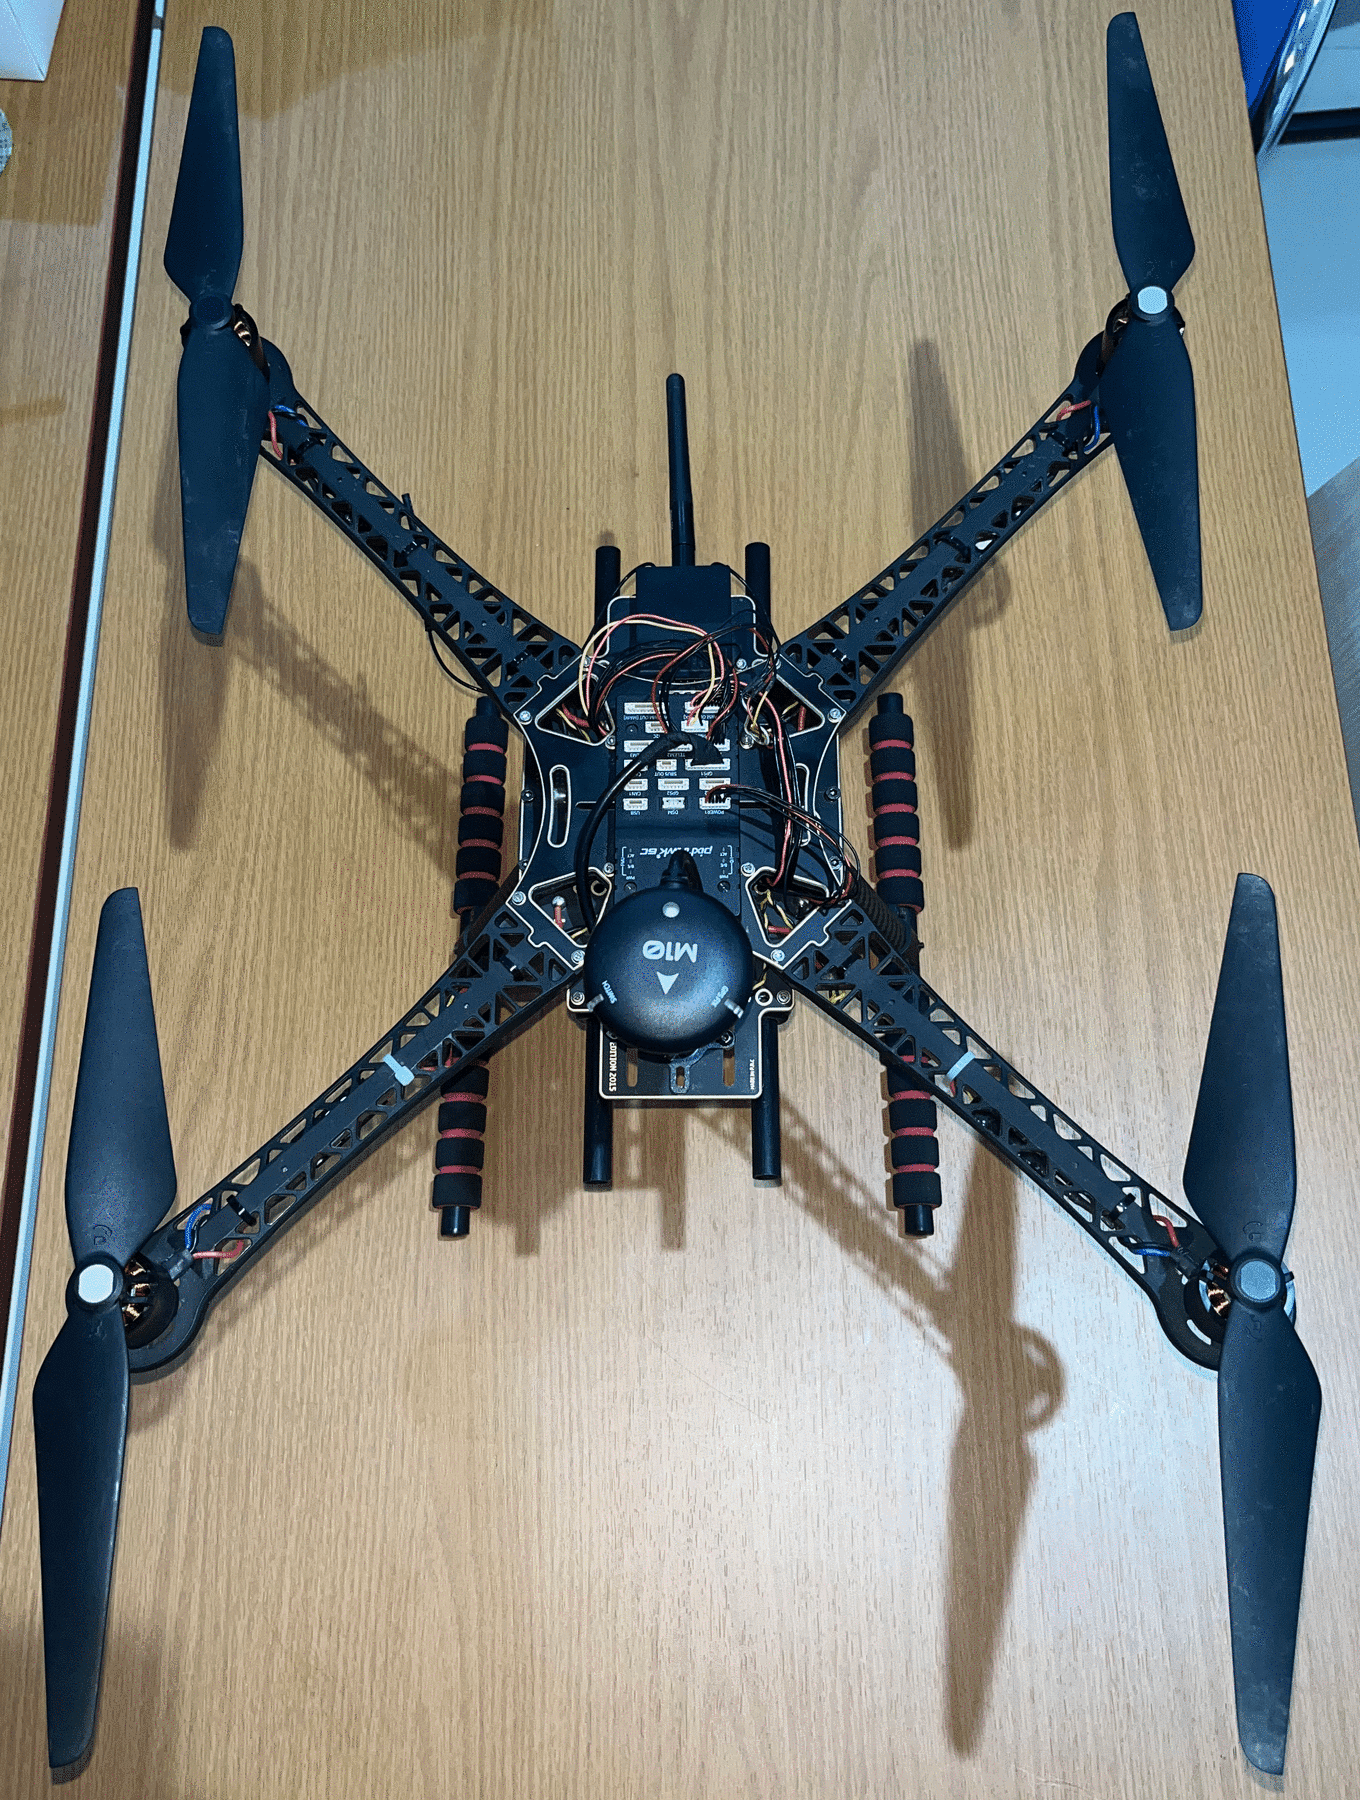
\includegraphics[width=0.9\linewidth]{bab3/drone_tampak_atas} 
			\caption{Drone Holybro S500 perspektif atas}
			\label{fig:drone_atas}
		\end{subfigure}
		\hfill
		\begin{subfigure}[b]{0.45\textwidth}
			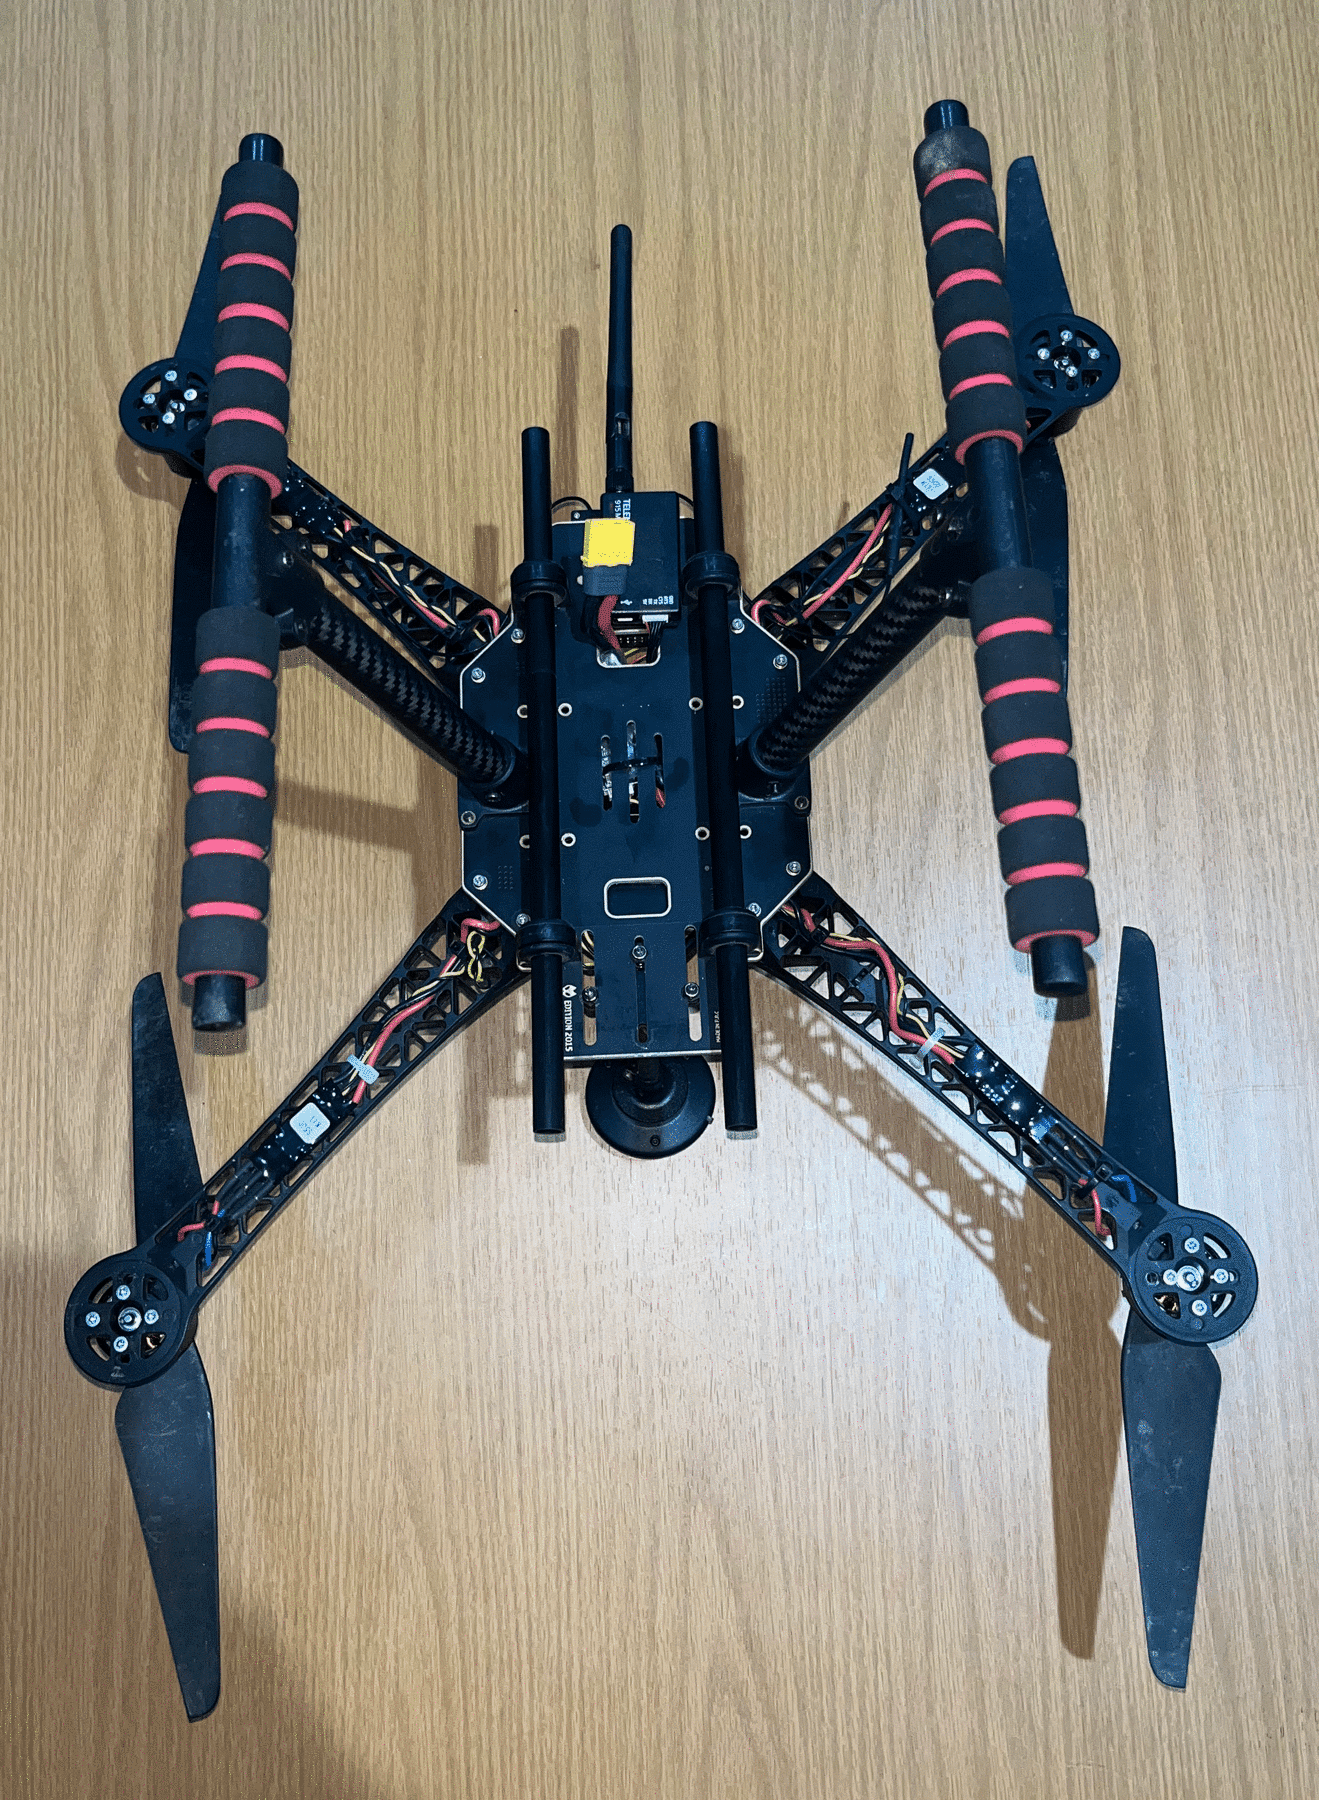
\includegraphics[width=0.9\linewidth]{bab3/drone_tampak_bawah} 
			\caption{Drone Holybro S500 perspektif bawah}
			\label{fig:drone_bawah}
		\end{subfigure}
	\end{figure}
	
	\item Integrasi Unit Komputasi dan Sensor: Raspberry Pi 5 dipasang sebagai \textit{companion computer} utama untuk menjalankan algoritma deteksi manusia. Unit ini dihubungkan dengan \textit{webcam} Logitech C922 melalui antarmuka USB 3.0 untuk menjamin transmisi data visual berkecepatan tinggi.
	\begin{figure}[H]
		\centering
		\begin{subfigure}[b]{0.45\textwidth}
			\centering
			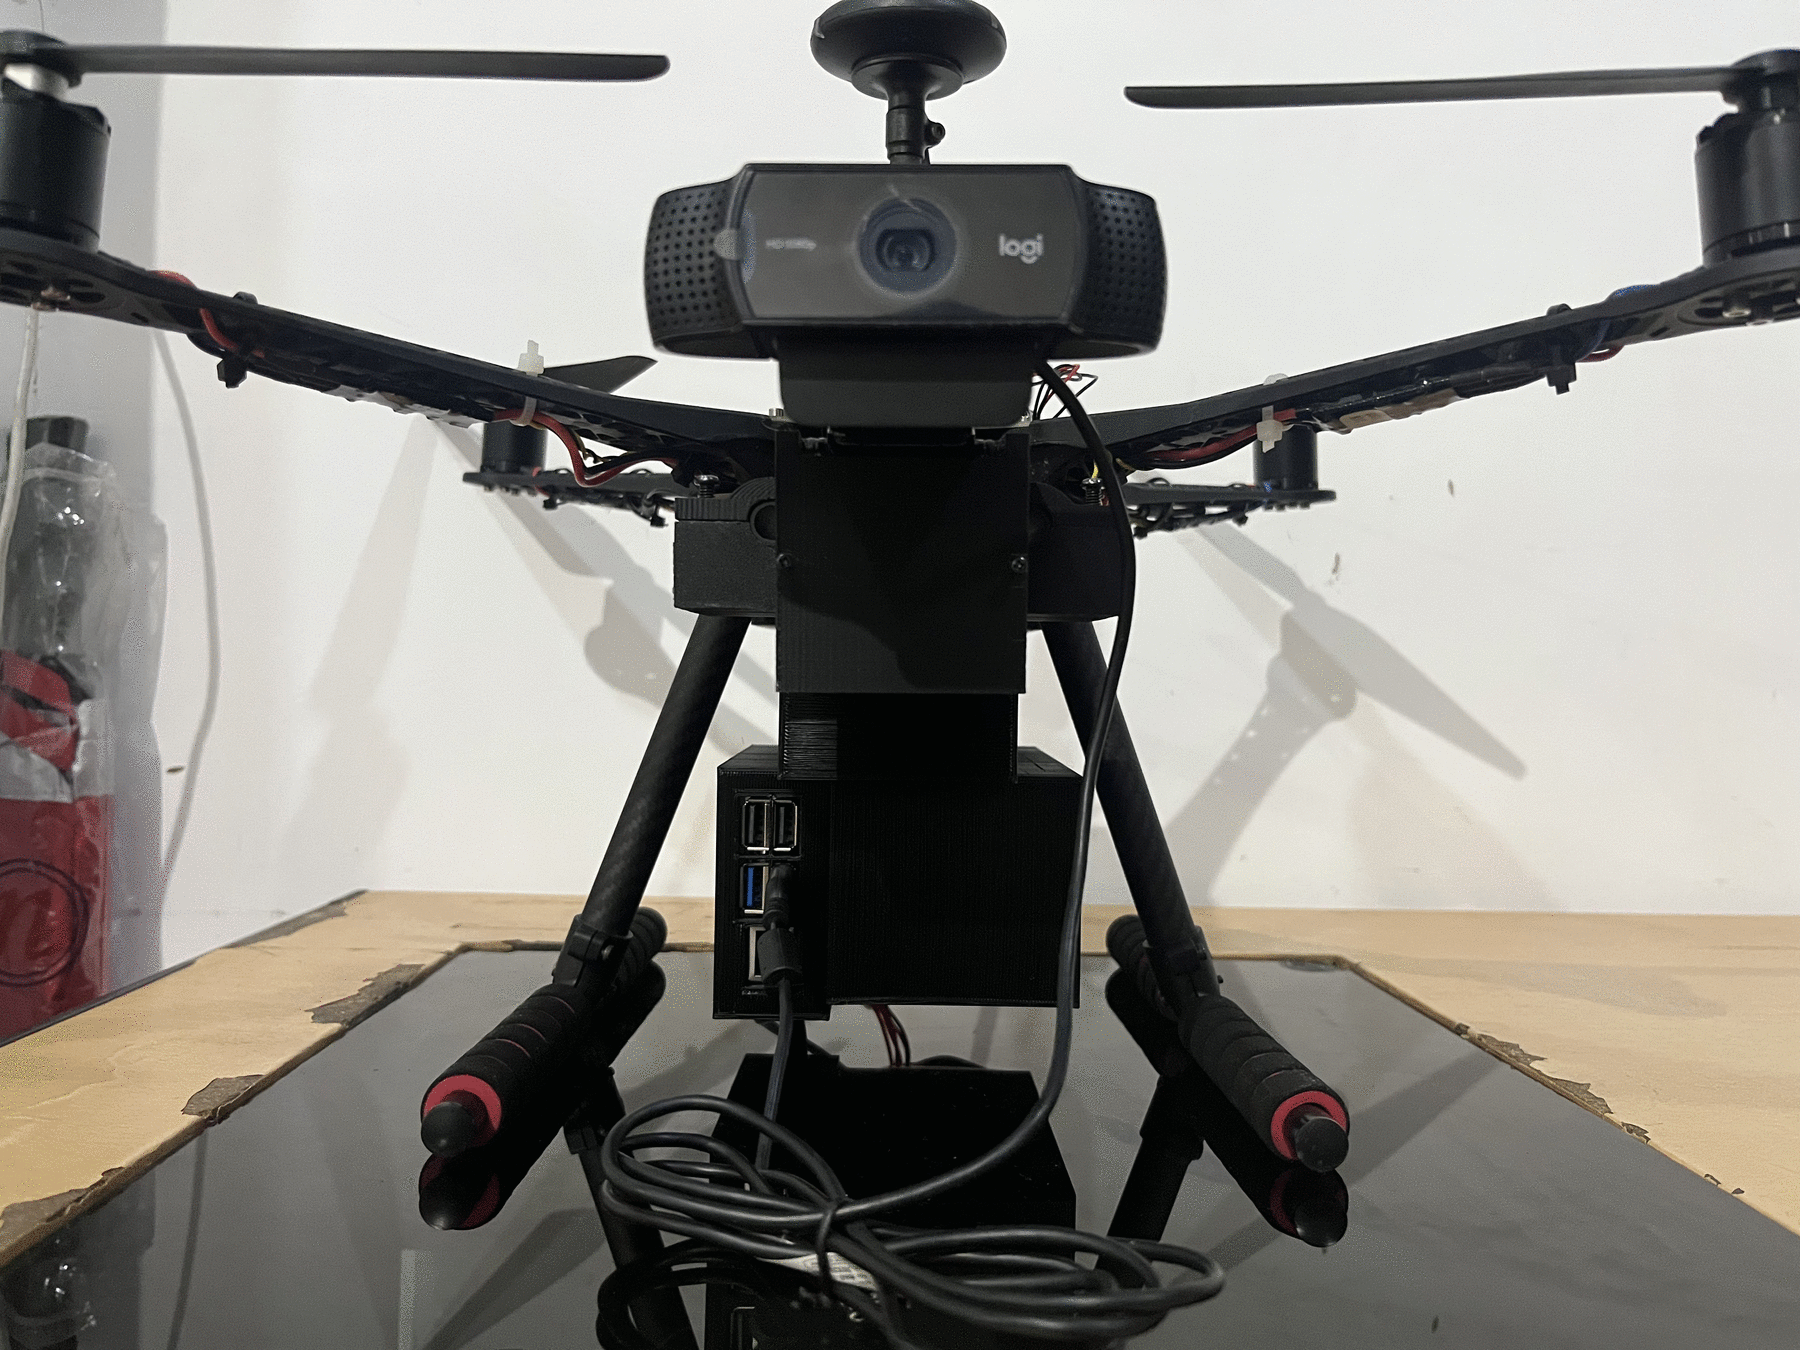
\includegraphics[width=\linewidth]{bab3/integrasi_webcam_rpi5_depan}
			\caption{Desain Awal}
		\end{subfigure}
		\hfill
		\begin{subfigure}[b]{0.45\textwidth}
			\centering
			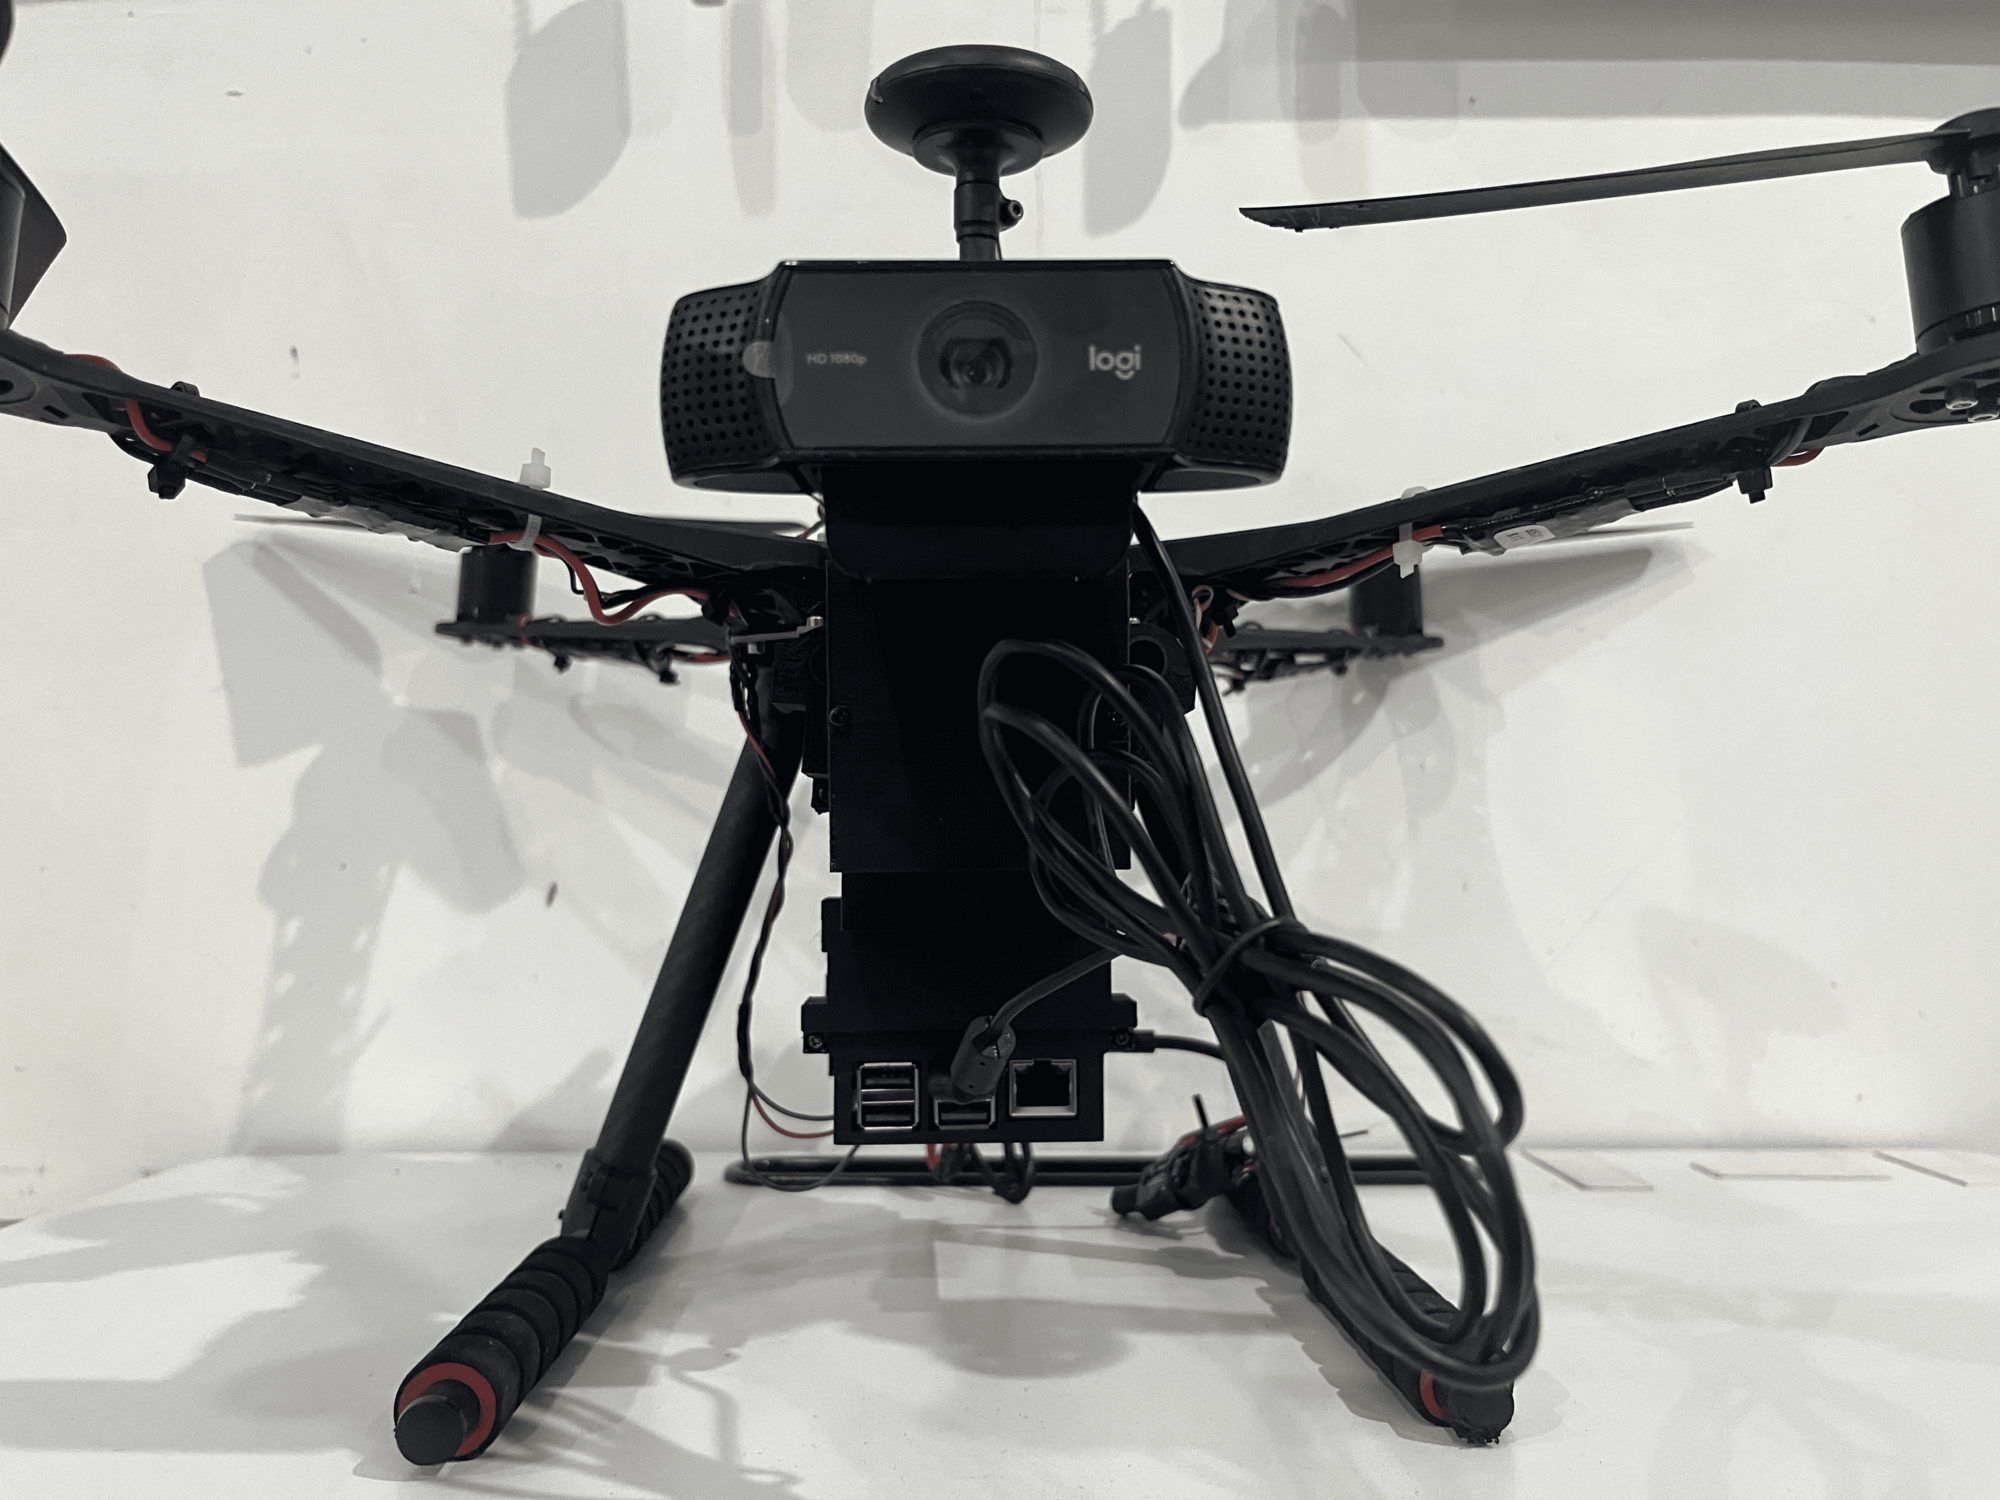
\includegraphics[width=\linewidth]{bab3/integrasi_webcam_rpi5_depan_desainbaru}
			\caption{Desain Baru}
		\end{subfigure}
		\caption{Integrasi Raspberry Pi 5 dan Webcam Logitech C922 depan}
		\label{fig:integrasi_rpi5_webcam_depan}
	\end{figure}
	
	\item Implementasi Sistem Daya dan Baterai: Untuk mendukung kebutuhan daya komputasi Raspberry Pi 5 yang tinggi saat mengeksekusi algoritma YOLOv8, dipasang modul UBEC 5A Hobbywing. Sebelum dirangkai ke dalam sistem drone, dilakukan penyesuaian antarmuka daya dengan menyolder konektor XT60 pada modul UBEC 5A serta menyiapkan kabel percabangan XT60 \textit{Y-Splitter}. Modifikasi ini dilakukan agar modul daya dapat terhubung dengan baterai LiPo secara aman, presisi, dan bersifat \textit{plug-and-play}.
	
	\begin{figure}[H]
		\centering
		\begin{subfigure}[b]{0.45\textwidth}
			\centering
			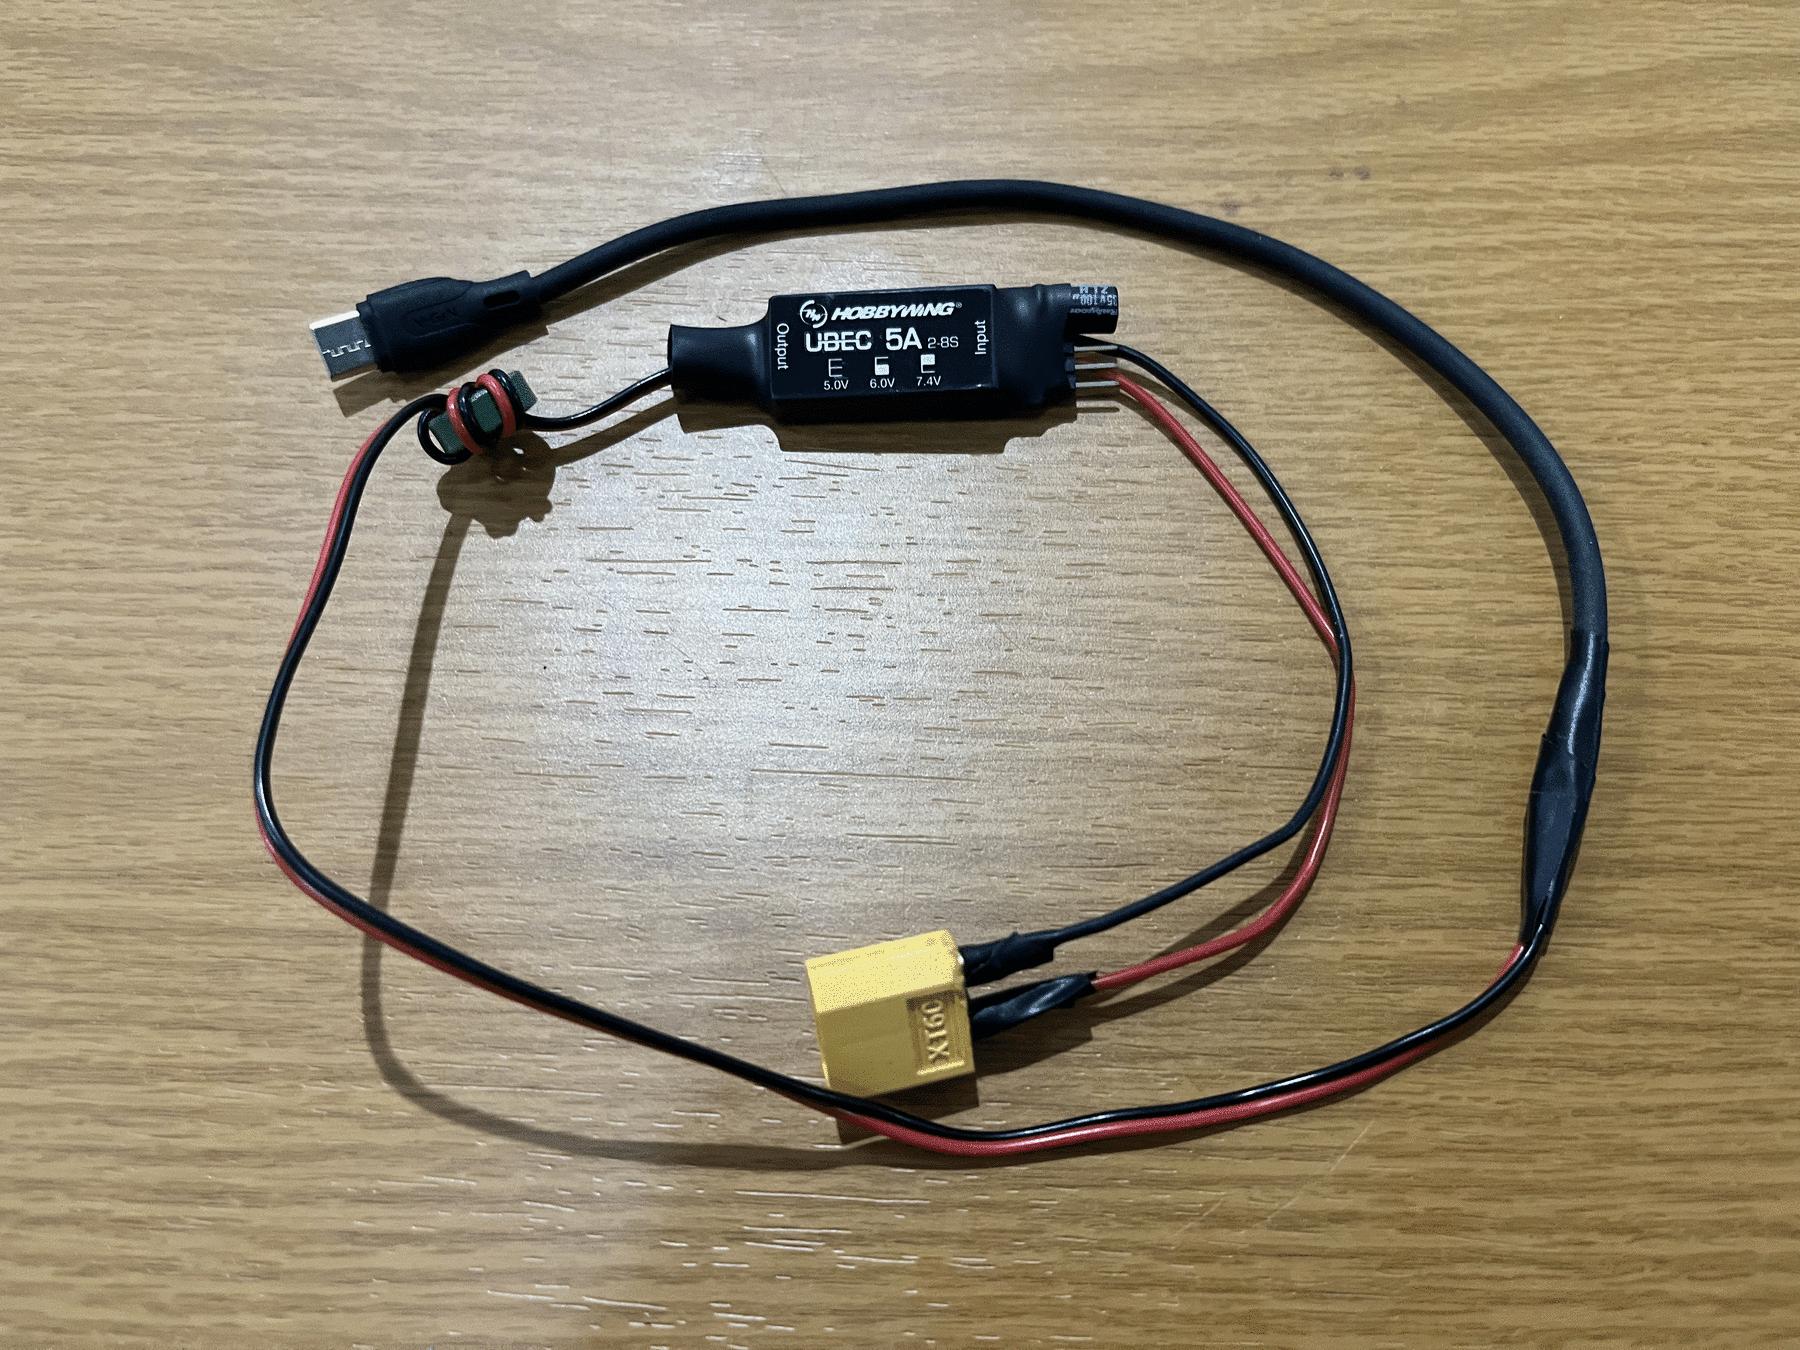
\includegraphics[width=0.9\linewidth]{bab3/ubec_xt60}
			\caption{Modul UBEC 5A yang telah disolder konektor XT60}
			\label{fig:ubec_soldered_real}
		\end{subfigure}
		\hfill
		\begin{subfigure}[b]{0.45\textwidth}
			\centering
			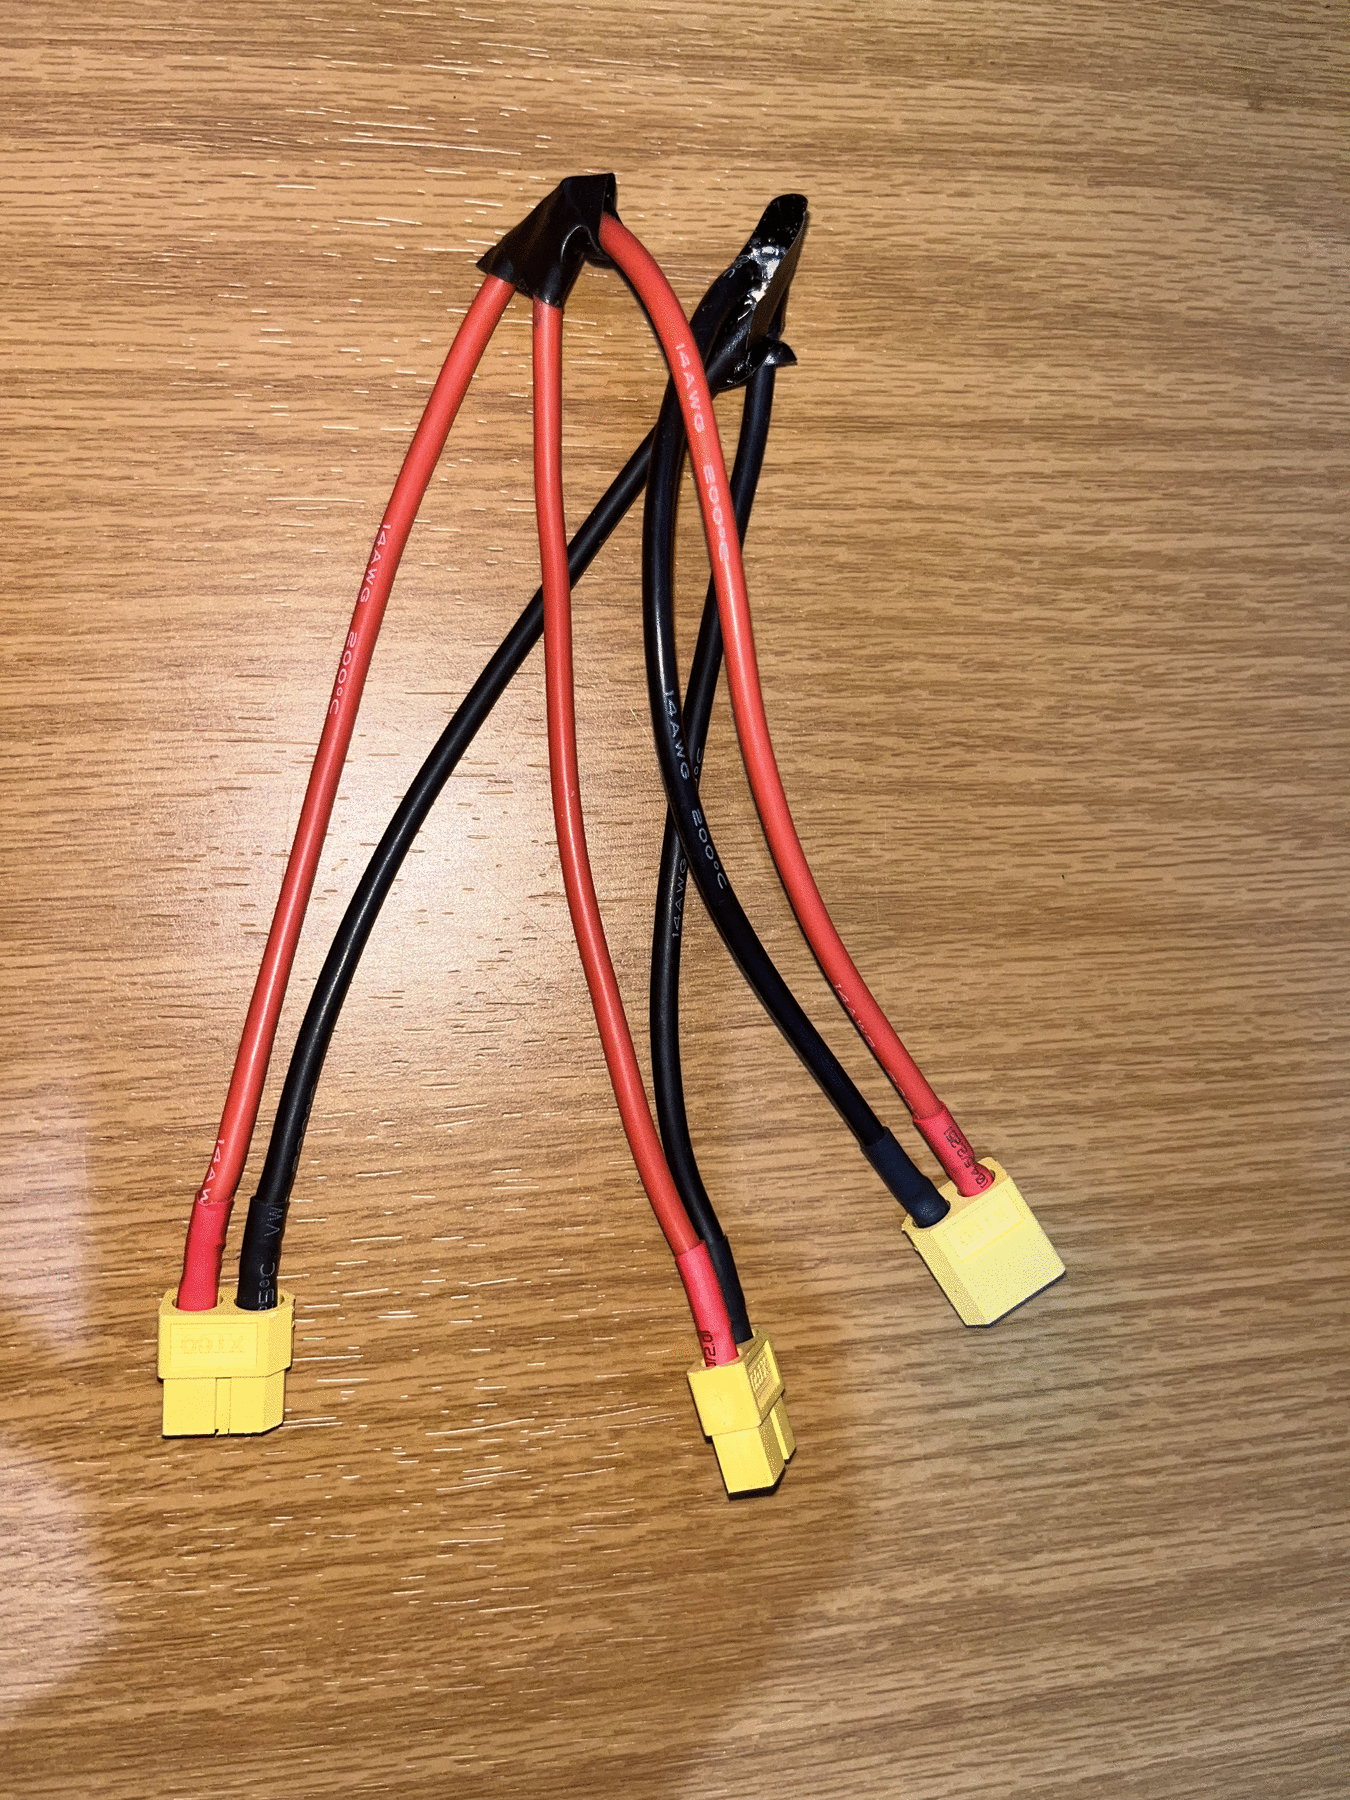
\includegraphics[width=0.9\linewidth]{bab3/xt60_y_splitter}
			\caption{Kabel percabangan daya XT60 \textit{Y-Splitter}}
			\label{fig:xt60_ysplitter_real}
		\end{subfigure}
	\end{figure}
	
	Berdasarkan kesiapan komponen daya tersebut, implementasi sistem daya direalisasikan dan dapat dioperasikan dalam dua konfigurasi baterai:
	\begin{enumerate}
		\item Konfigurasi Baterai Tunggal (Paralel): Modul UBEC 5A dihubungkan secara paralel dengan jalur daya utama (\textit{Power Distribution Board} / PDB) menggunakan konektor XT60 \textit{Y-Splitter}. Pada implementasi ini, komputasi Raspberry Pi 5 dan motor \textit{brushless} disuplai oleh satu baterai LiPo 4S utama.
		\begin{figure}[H]
			\centering
			\begin{subfigure}[b]{0.45\textwidth}
				\centering
				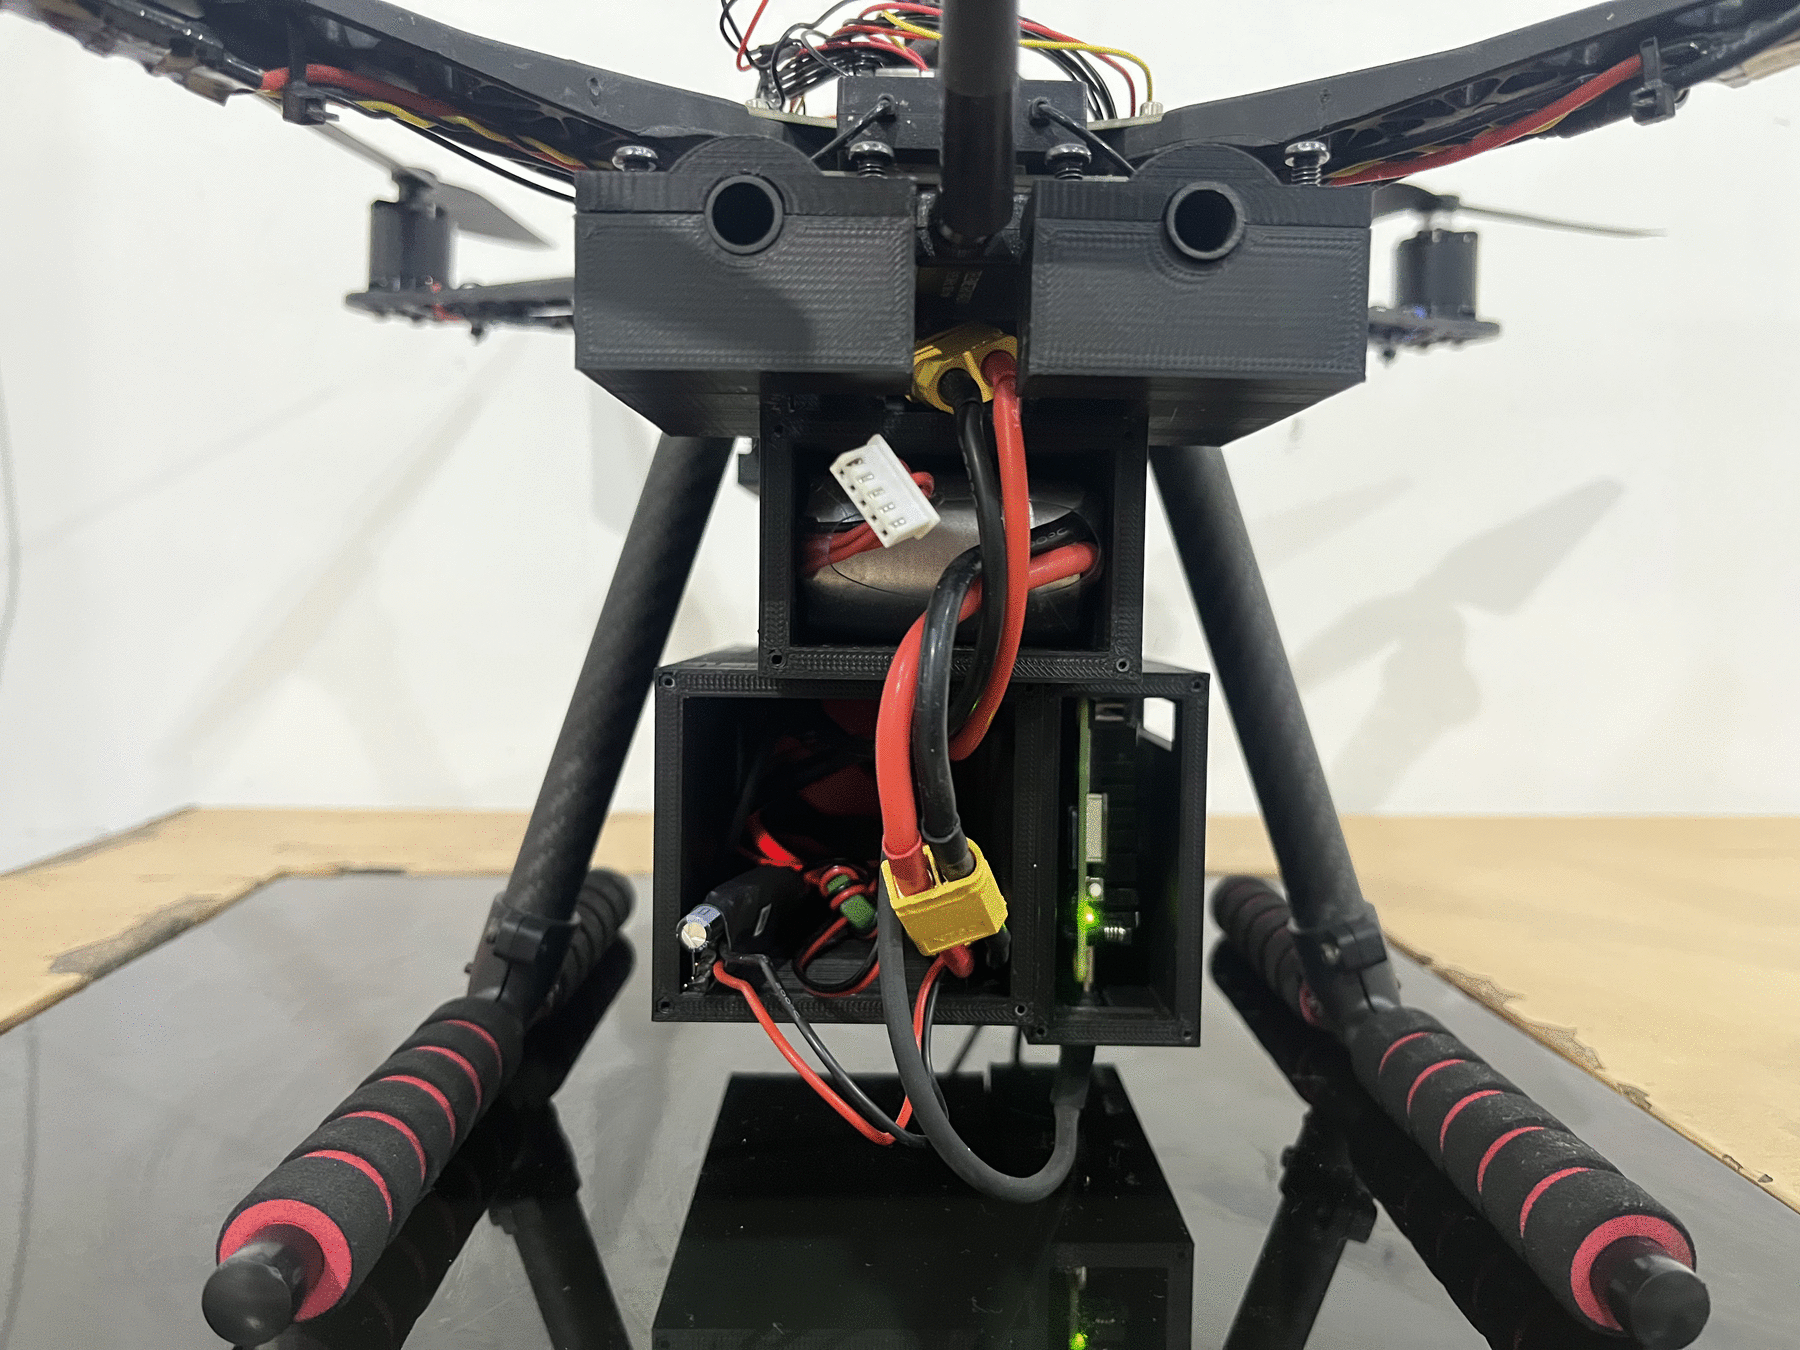
\includegraphics[width=0.9\linewidth]{bab3/konfig_baterai_tunggal_nc}
				\caption{Tanpa Penutup (Desain Awal)}
				\label{fig:baterai-tunggal-real-no-case}
			\end{subfigure}
			\hfill
			\begin{subfigure}[b]{0.45\textwidth}
				\centering
				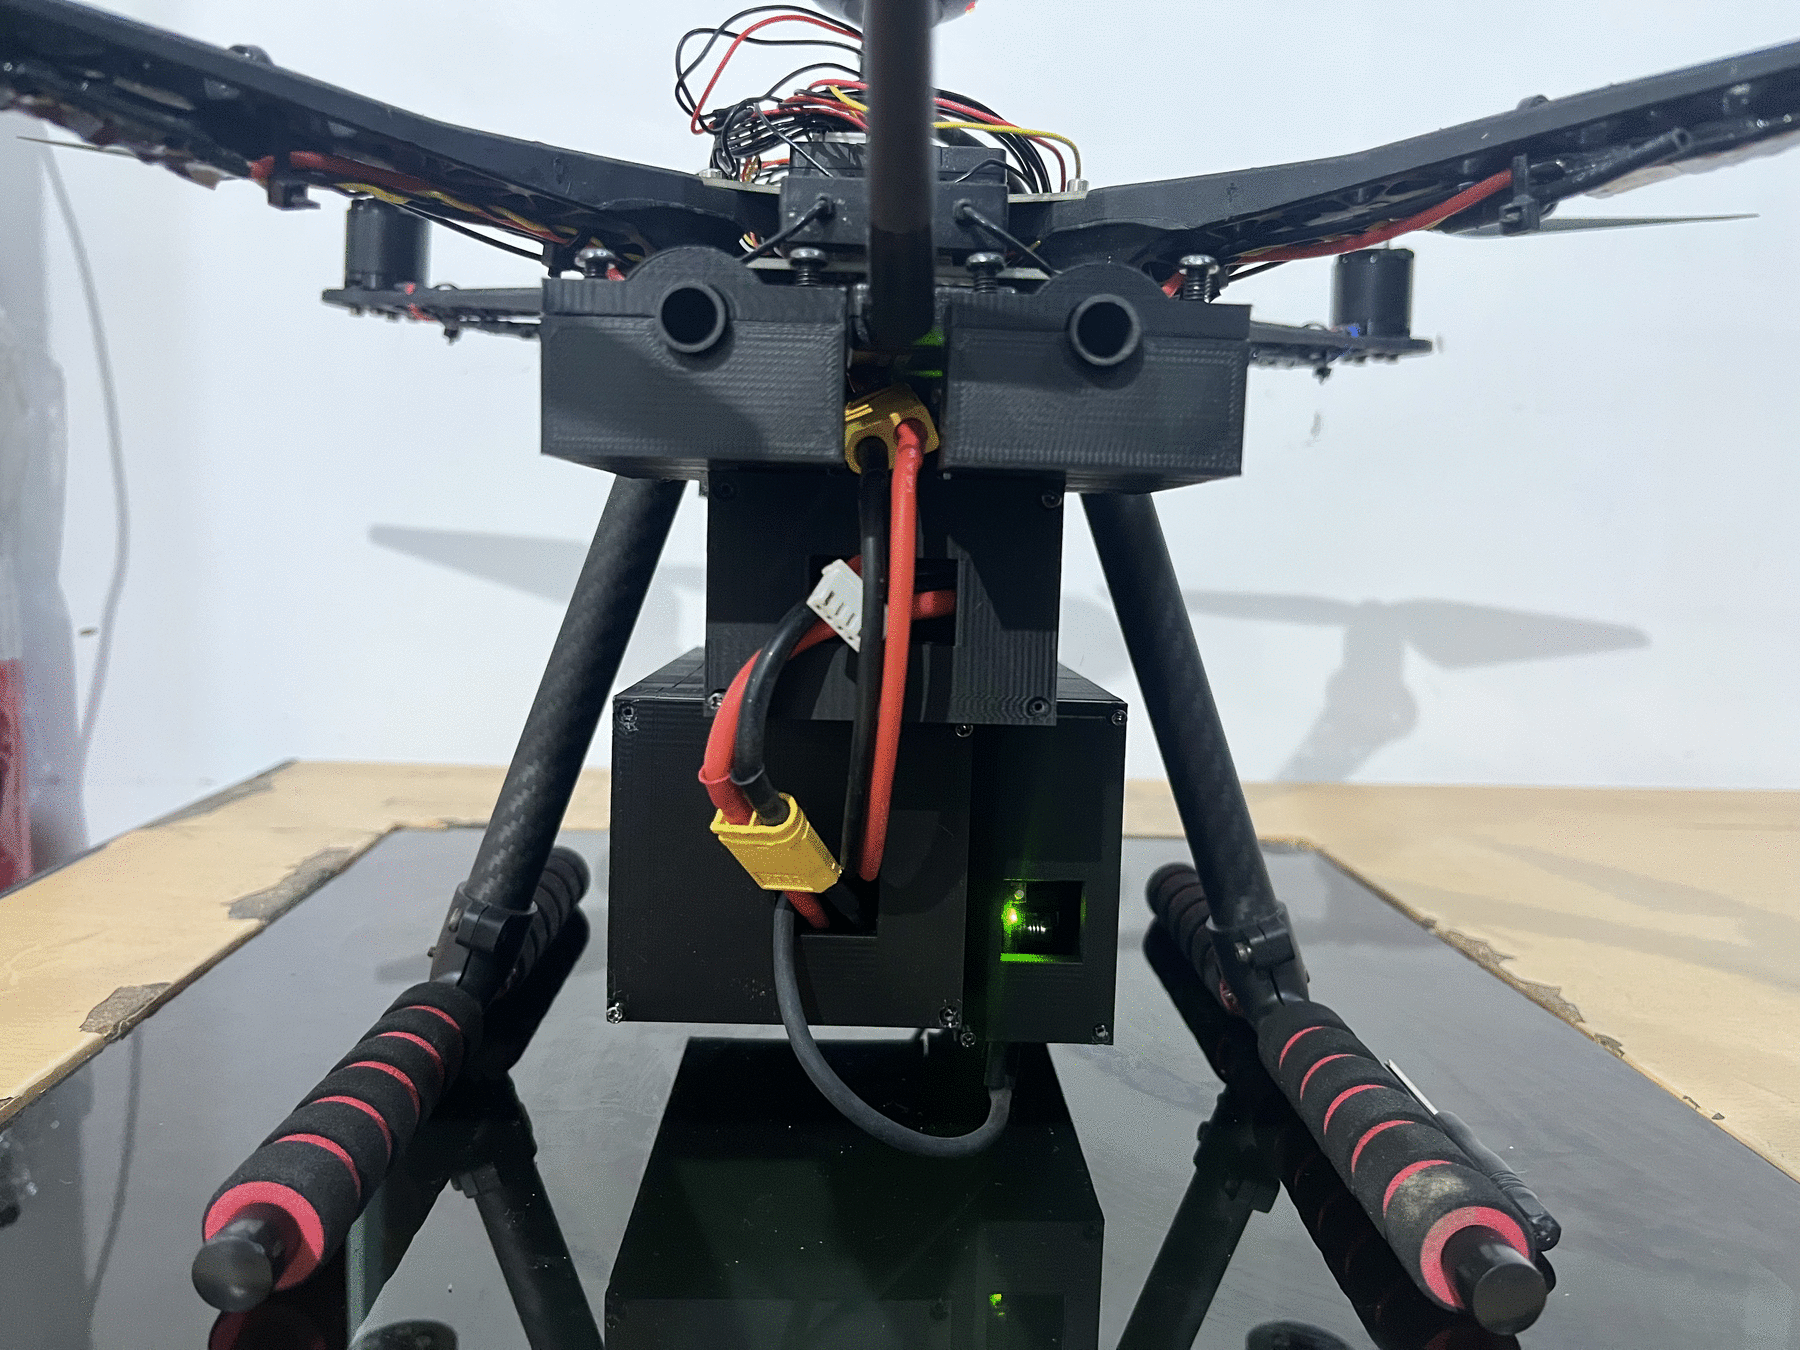
\includegraphics[width=0.9\linewidth]{bab3/konfig_baterai_tunggal_wc}
				\caption{Dengan Penutup (Desain Awal)}
				\label{fig:baterai-tunggal-real-with-case}
			\end{subfigure}
			
			\vspace{0.5cm}
			
			\begin{subfigure}[b]{0.45\textwidth}
				\centering
				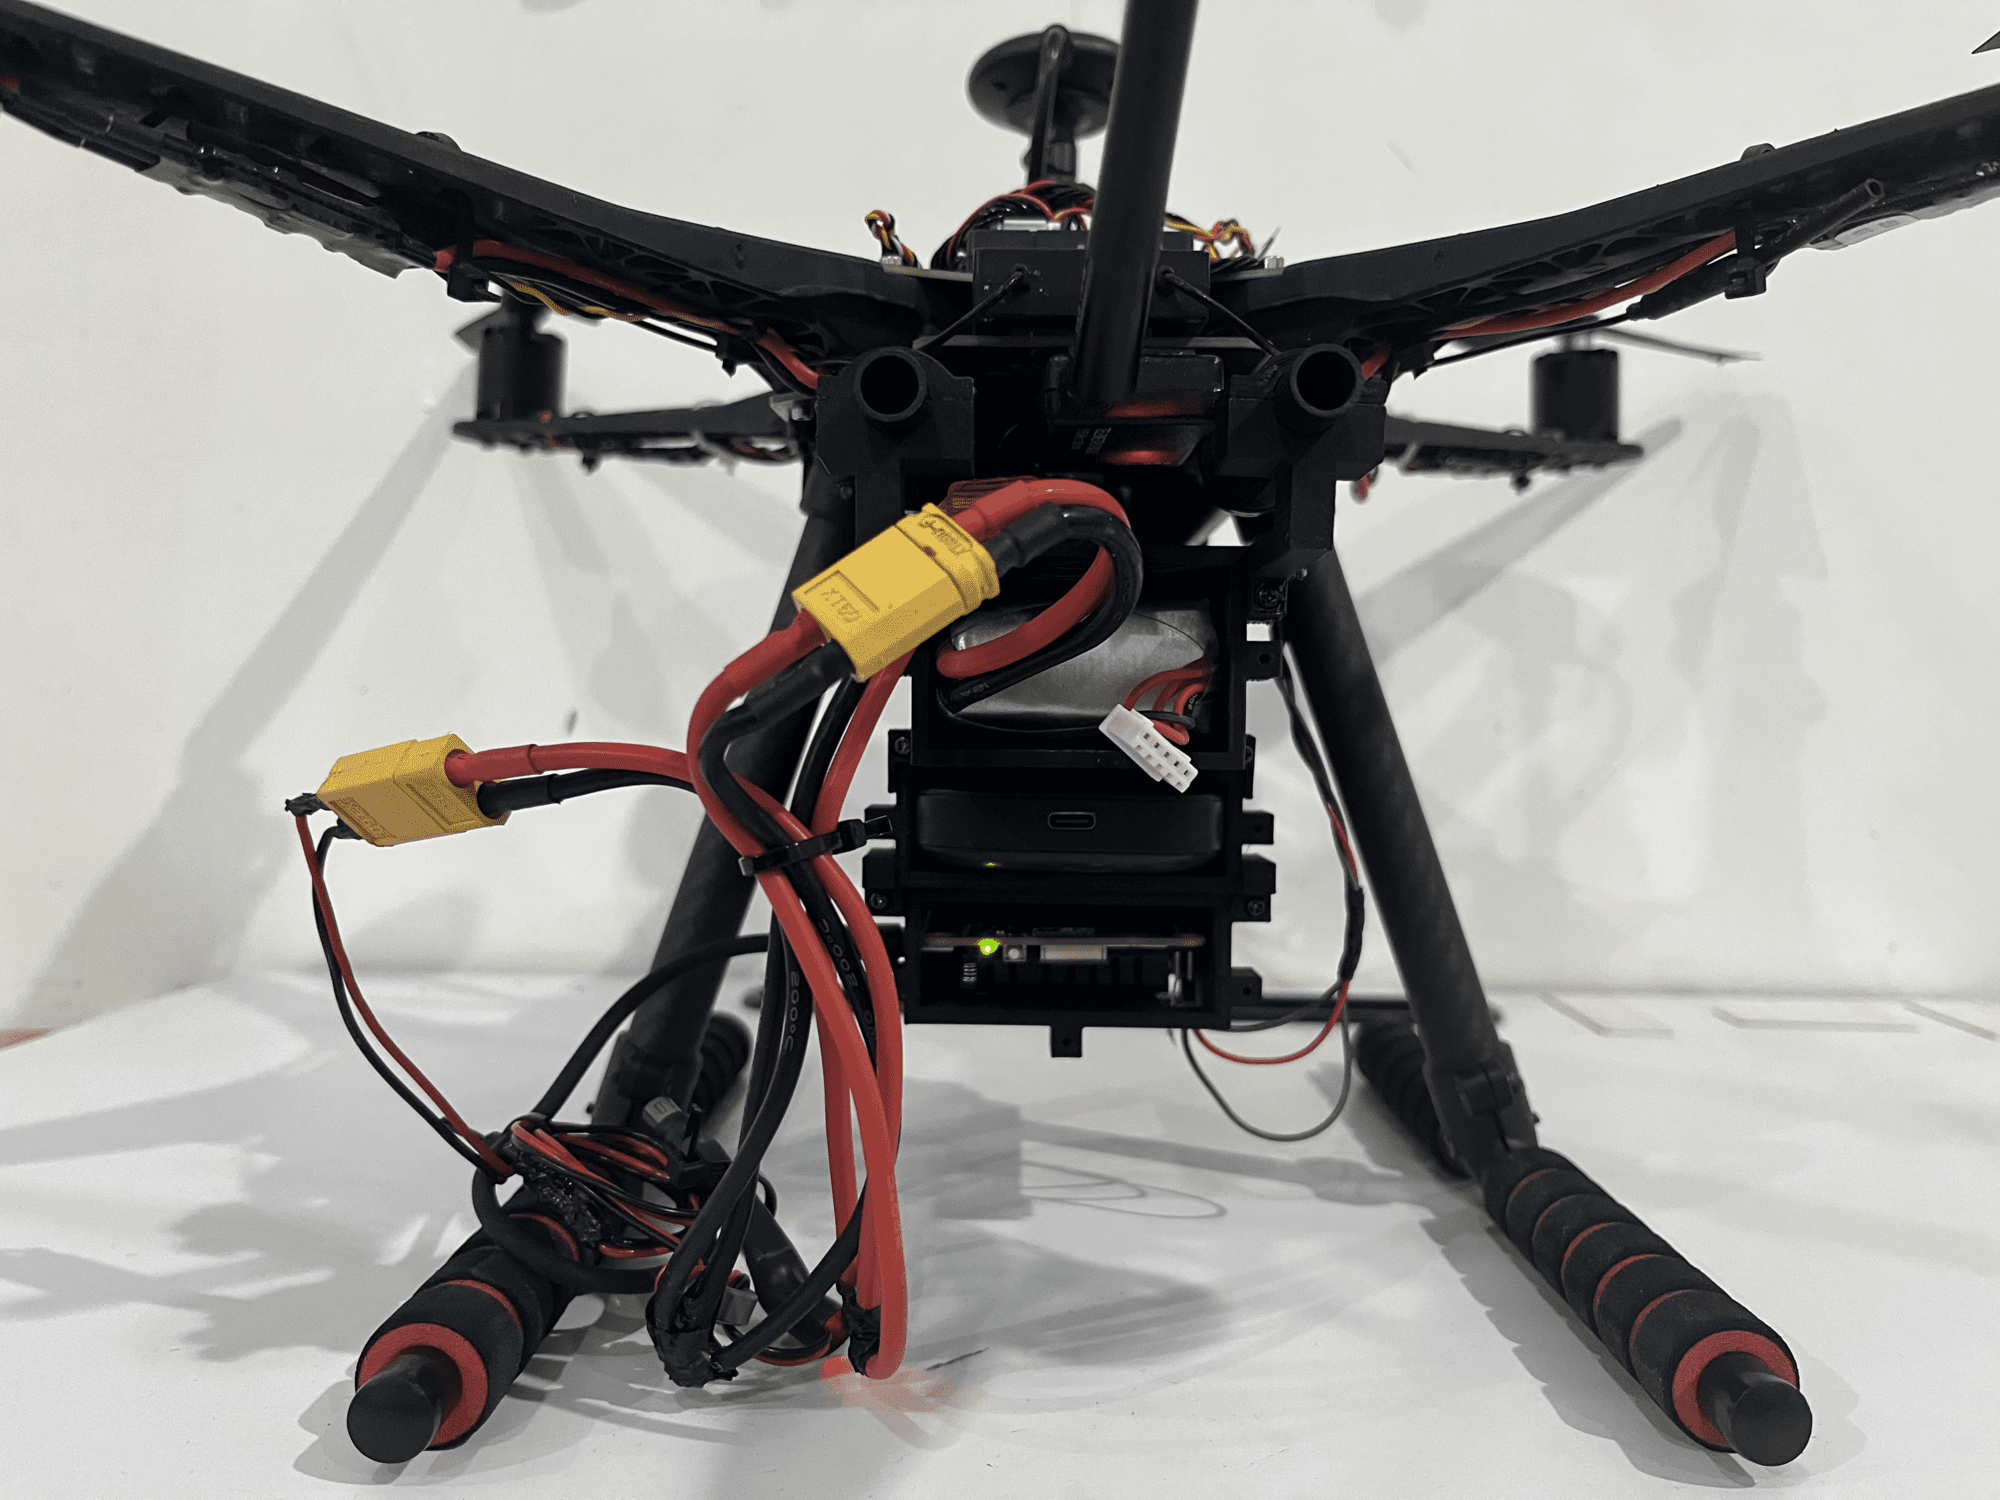
\includegraphics[width=0.9\linewidth]{bab3/konfig_baterai_tunggal_nc_desainbaru}
				\caption{Tanpa Penutup (Desain Baru)}
			\end{subfigure}
			\hfill
			\begin{subfigure}[b]{0.45\textwidth}
				\centering
				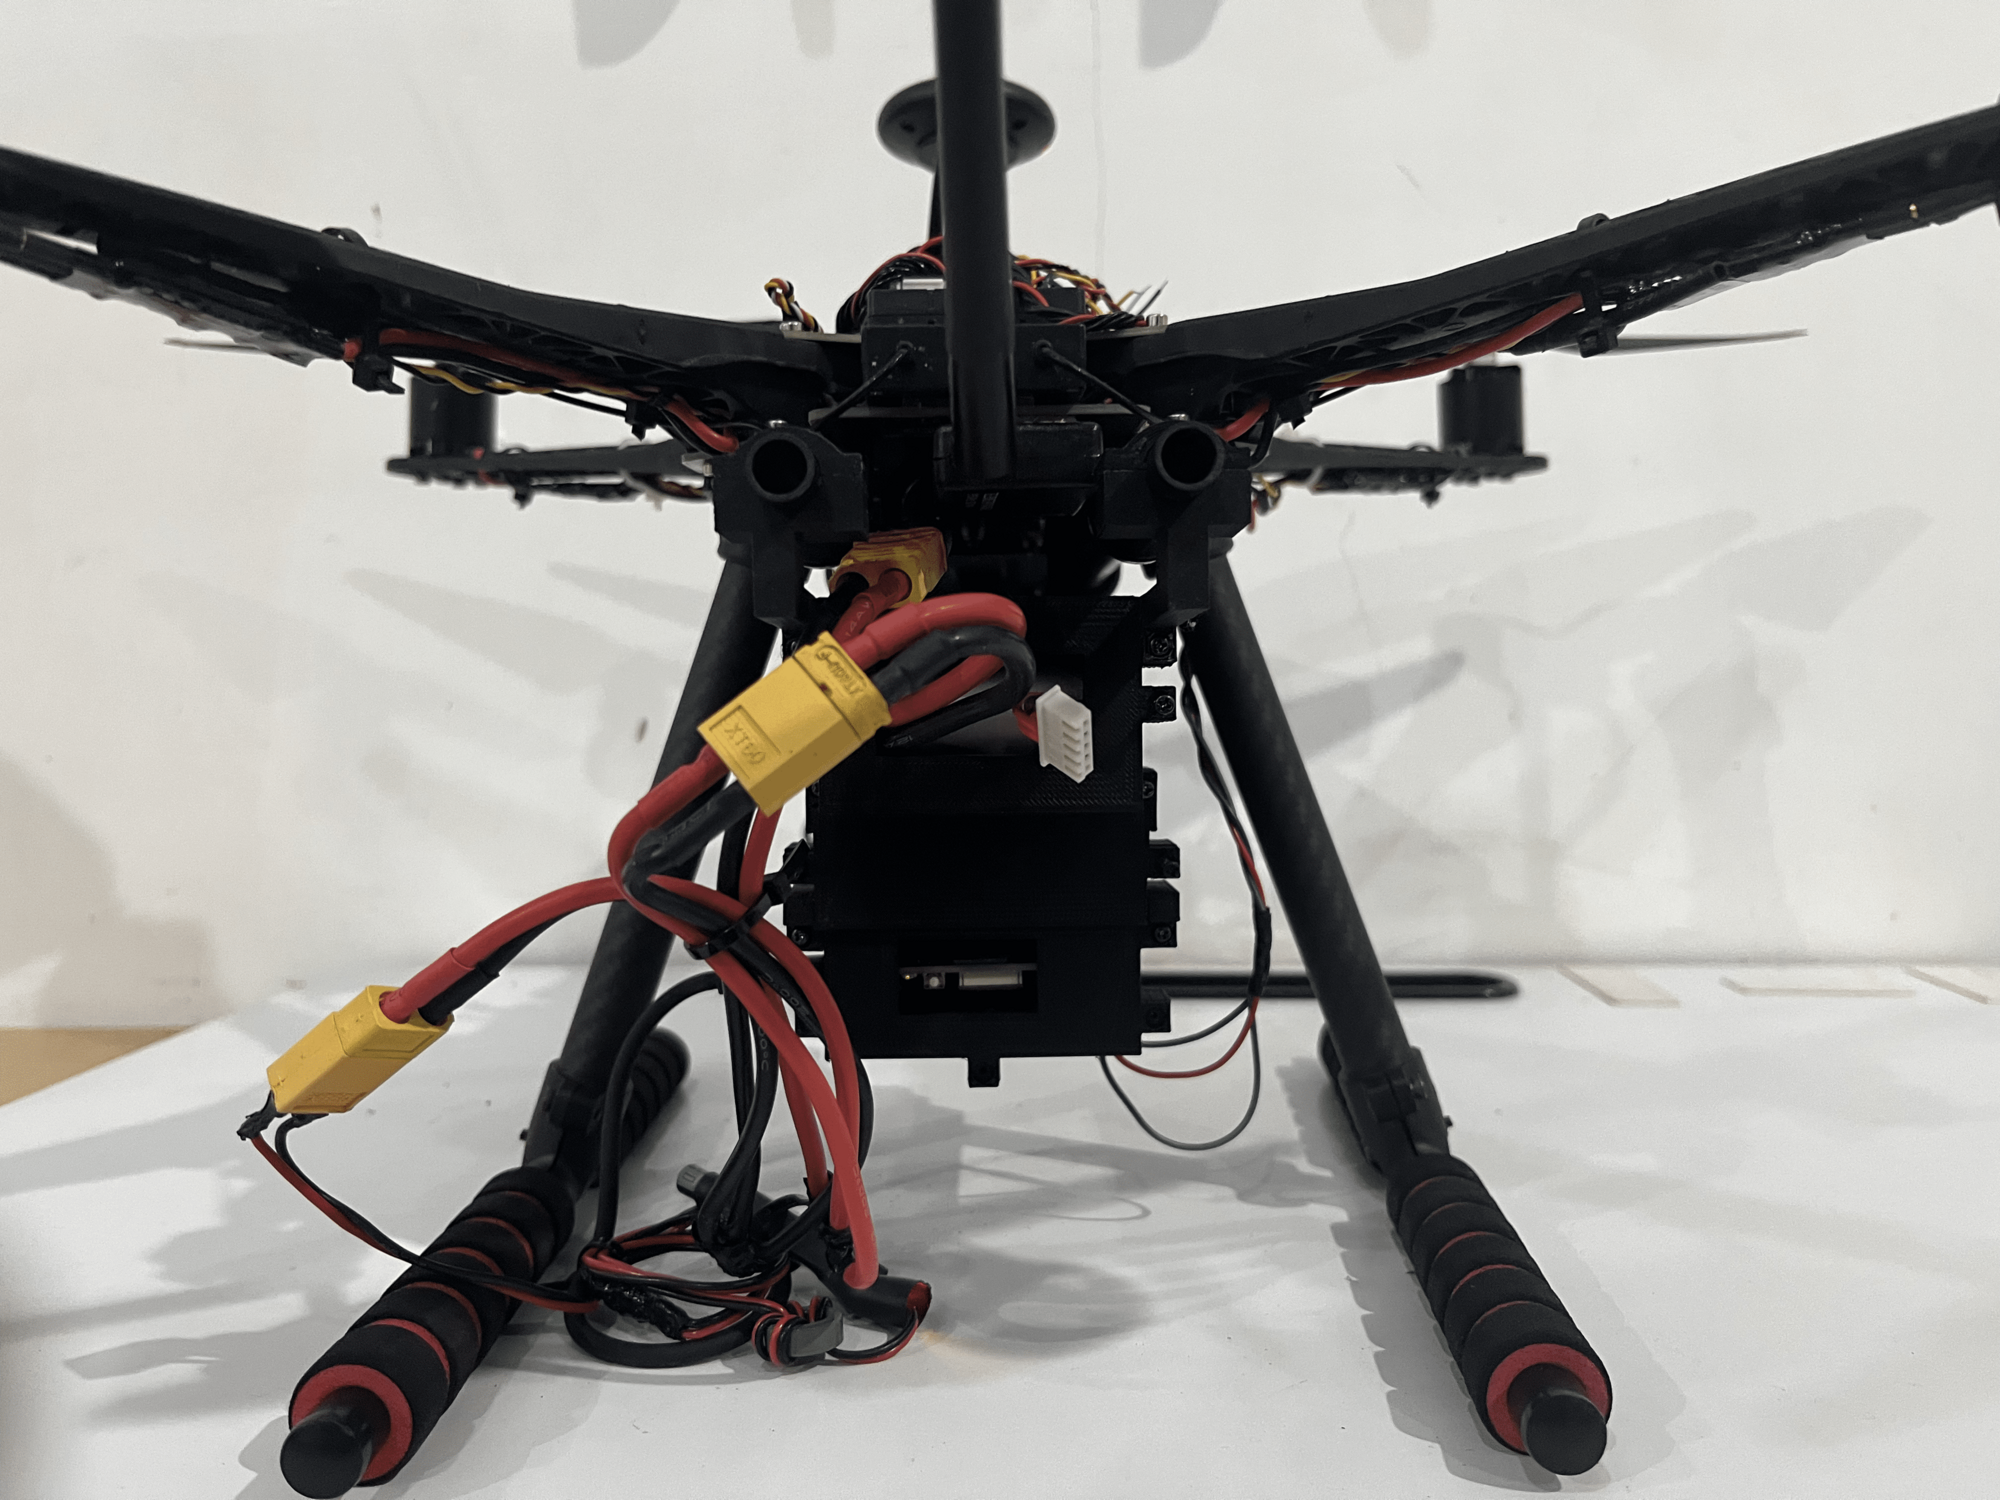
\includegraphics[width=0.9\linewidth]{bab3/konfig_baterai_tunggal_wc_desainbaru}
				\caption{Dengan Penutup (Desain Baru)}
			\end{subfigure}
			\caption{Realisasi Fisik Konfigurasi Baterai Tunggal (Paralel)}
		\end{figure}
		\item Konfigurasi Baterai Ganda (Terisolasi): Modul UBEC 5A dihubungkan langsung ke baterai LiPo sekunder yang terpisah dari PDB. Implementasi fisik ini dilakukan untuk mengisolasi catu daya \textit{companion computer} dari potensi penurunan tegangan sementara (\textit{voltage sag}) akibat lonjakan arus dari motor propulsi saat drone bermanuver ekstrem.
		\begin{figure}[H]
			\centering
			\begin{subfigure}[b]{0.45\textwidth}
				\centering
				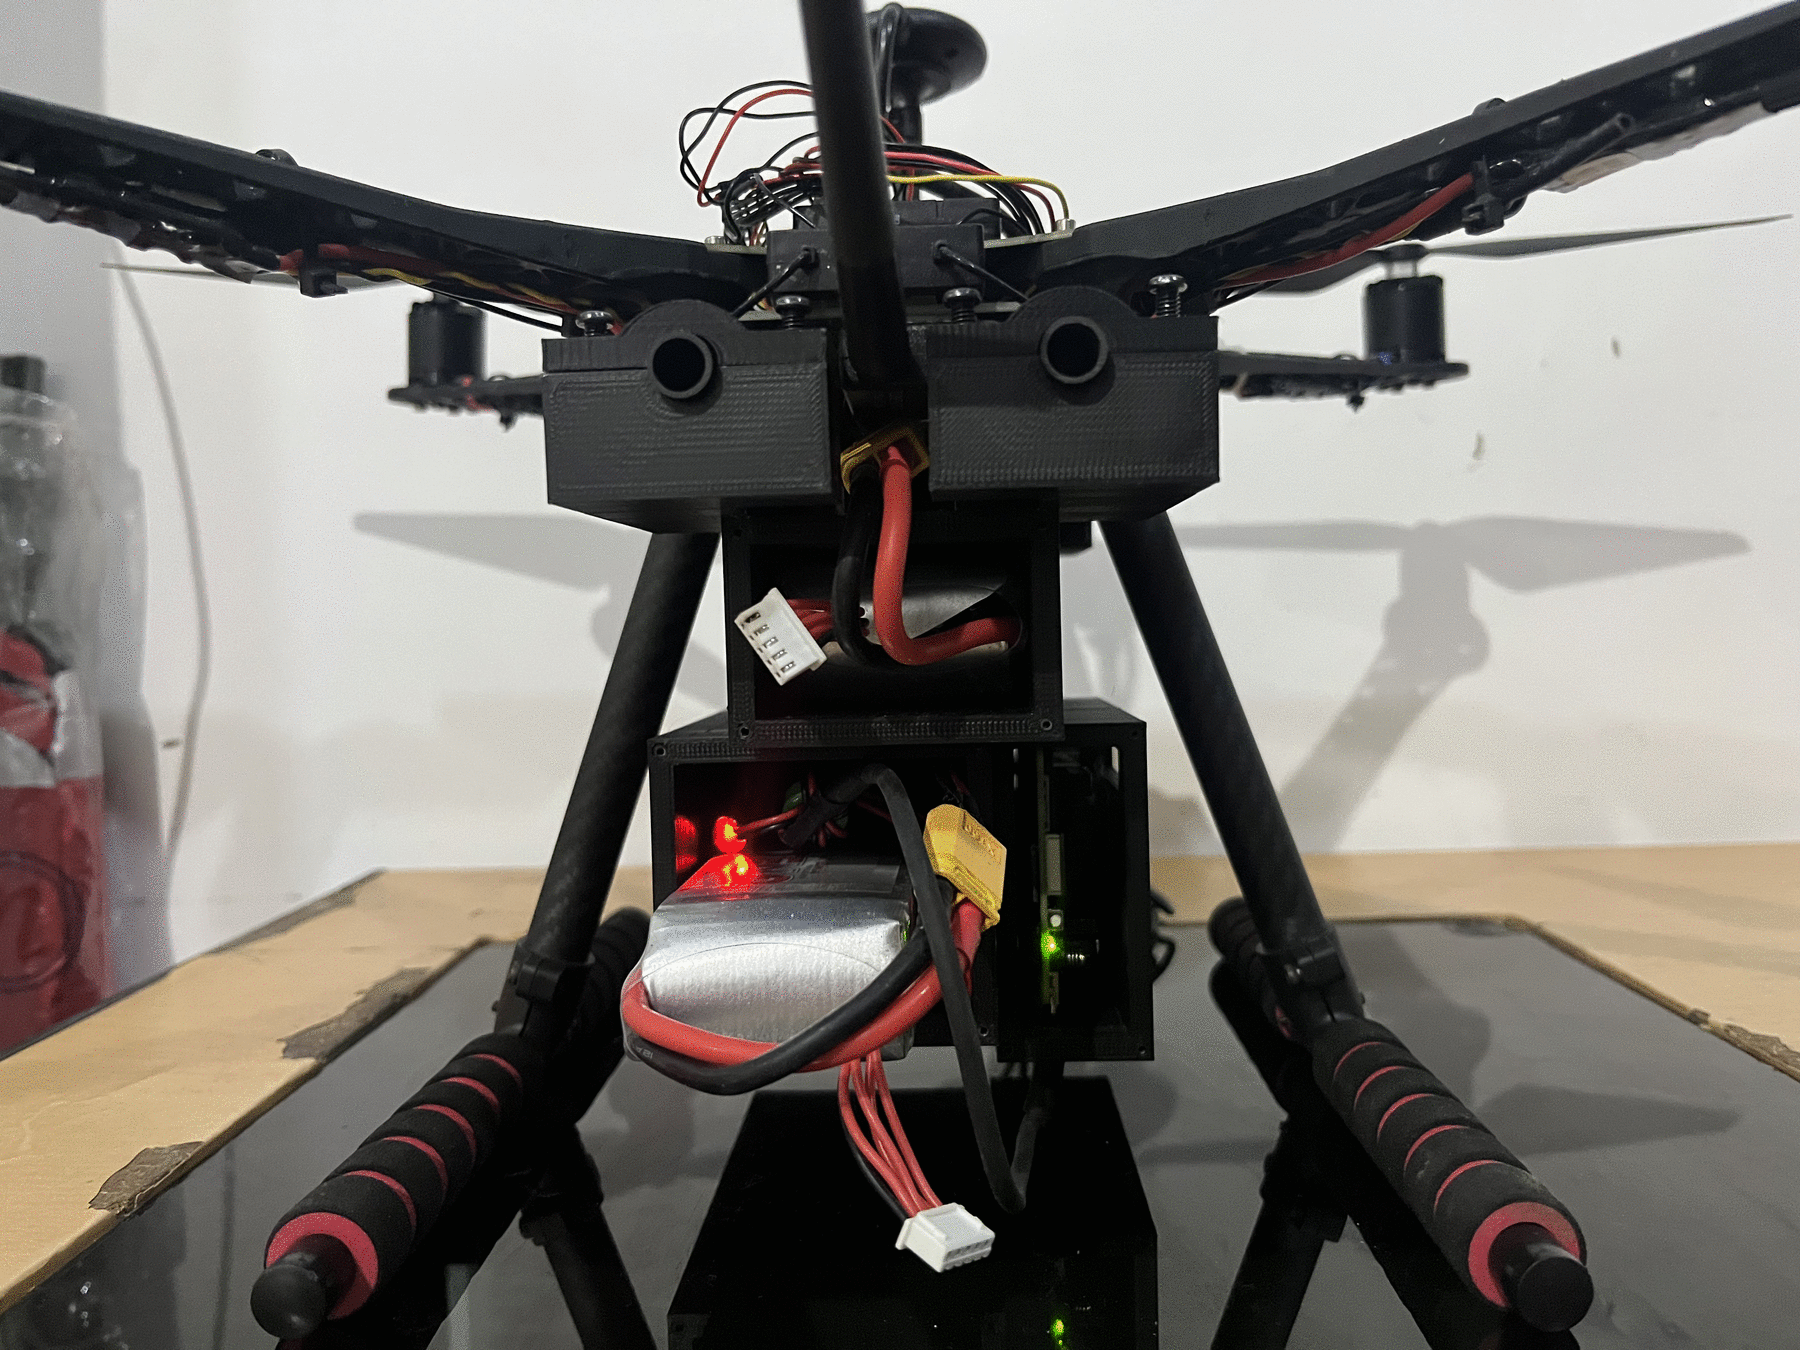
\includegraphics[width=0.9\linewidth]{bab3/konfig_baterai_ganda_nc} % Sesuaikan path
				\caption{Realisasi Fisik Konfigurasi Baterai Ganda (Terisolasi) Tanpa Penutup}
				\label{fig:baterai-ganda-real-no-case}
			\end{subfigure}
			\hfill
			\begin{subfigure}[b]{0.45\textwidth}
				\centering
				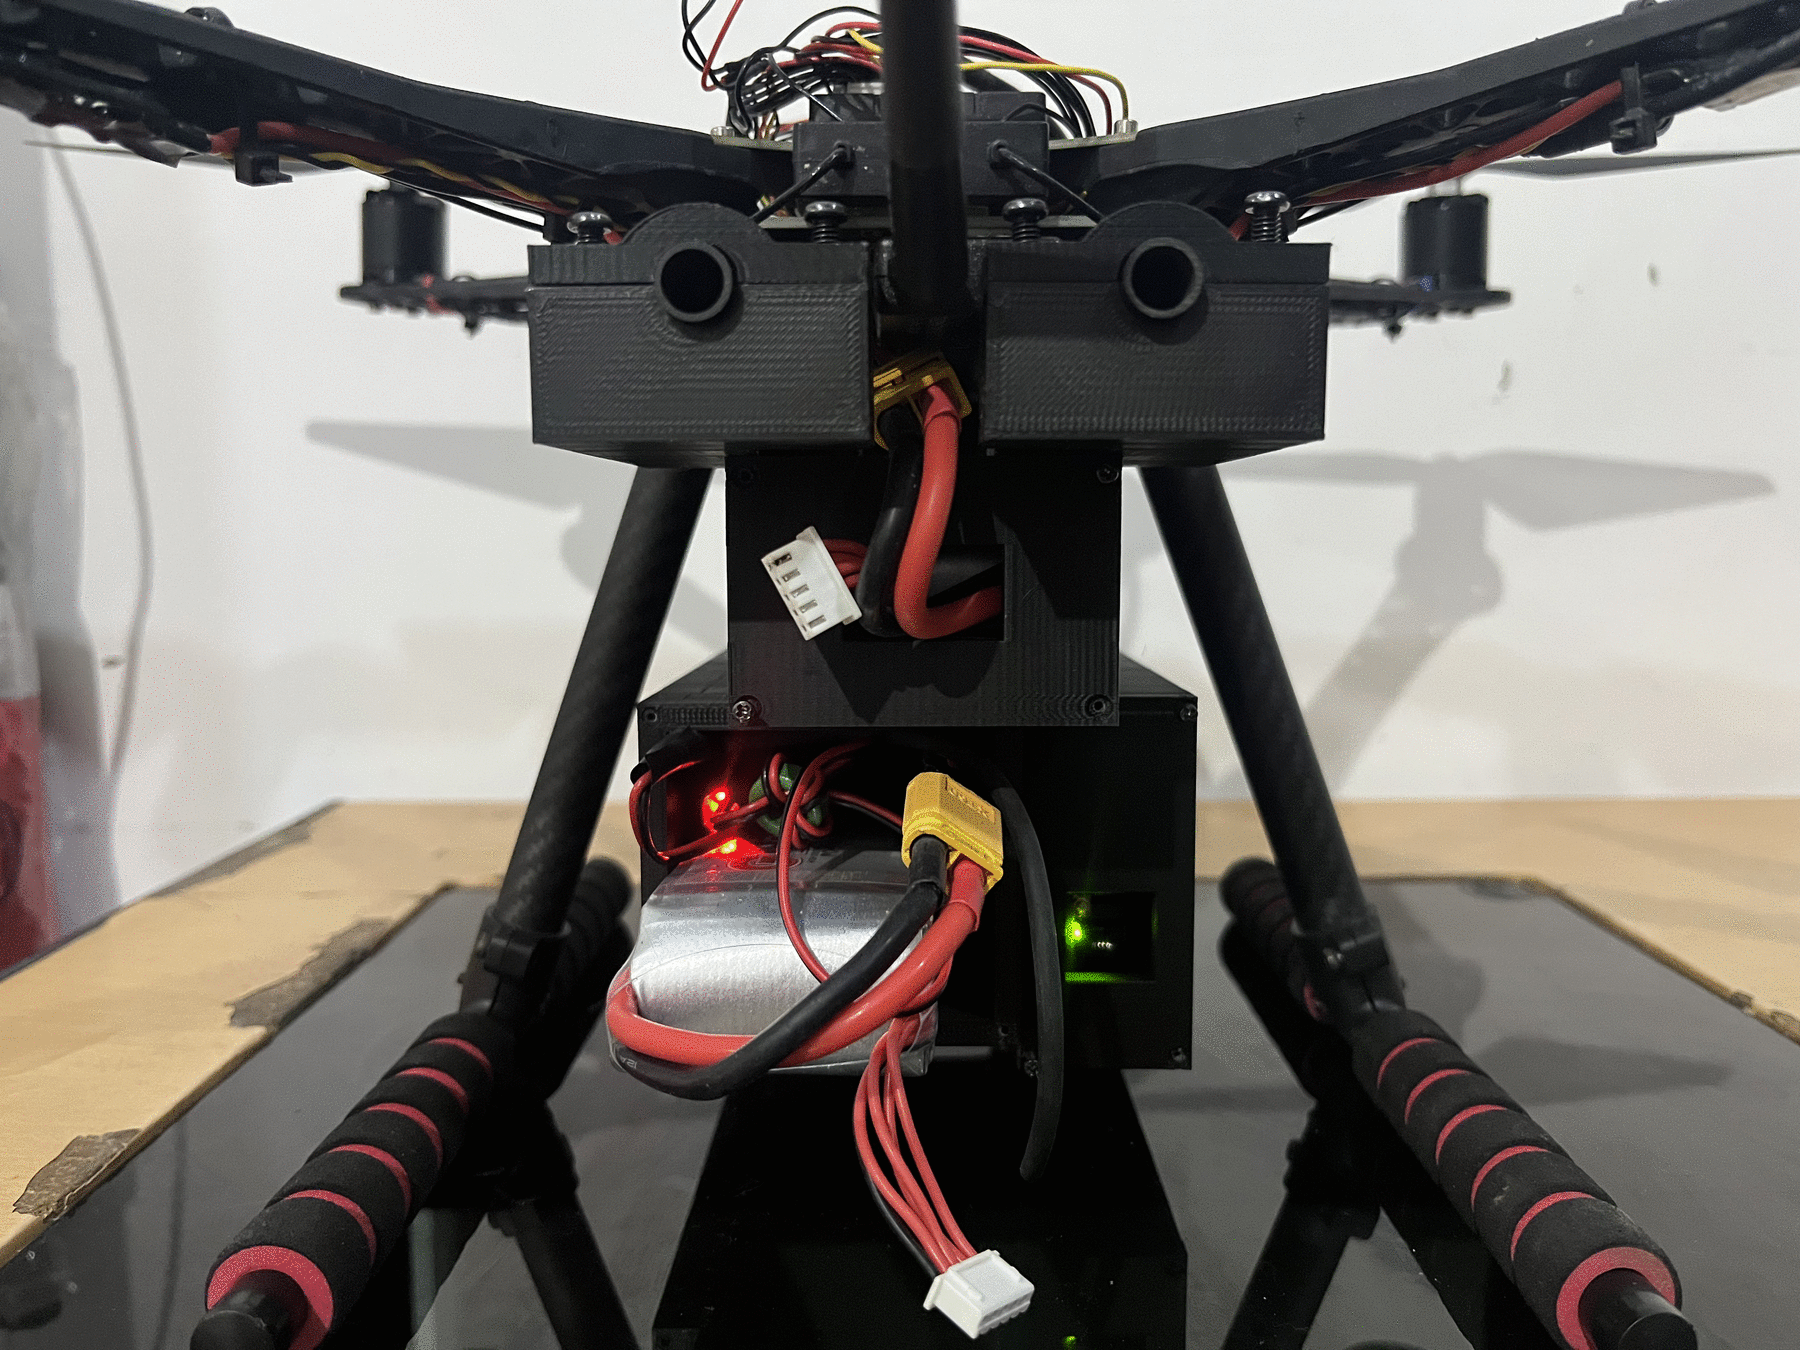
\includegraphics[width=0.9\linewidth]{bab3/konfig_baterai_ganda_wc} % Sesuaikan path
				\caption{Realisasi Fisik Konfigurasi Baterai Ganda (Terisolasi) Dengan Penutup}
				\label{fig:baterai-ganda-real-with-case}
			\end{subfigure}
		\end{figure}
	\end{enumerate}
	Melalui implementasi modul UBEC 5A pada kedua konfigurasi tersebut, suplai tegangan 5V ke Raspberry Pi terbukti tetap stabil selama proses inferensi berlangsung, sehingga berhasil mengatasi masalah malfungsi daya pada purwarupa awal.
	
	\item Konektivitas Data Telemetri:\\
	Komunikasi pertukaran pesan MAVLink antara Raspberry Pi 5 dan Pixhawk dikonfigurasi pada \textit{baud rate} 57600. Implementasi pengiriman data telemetri ini dapat diakses secara \textit{real-time} baik menggunakan antarmuka Serial USB melalui \textit{port} \texttt{/dev/ttyUSB0}, maupun menggunakan jalur Serial UART melalui \textit{port} \texttt{/dev/ttyAMA0}. Kedua jalur komunikasi tersebut memberikan kinerja yang ekuivalen dalam pengujian integrasi kontrol otonom.
	
	\begin{figure}[H]
		\centering
		\begin{subfigure}[b]{0.45\textwidth}
			\centering
			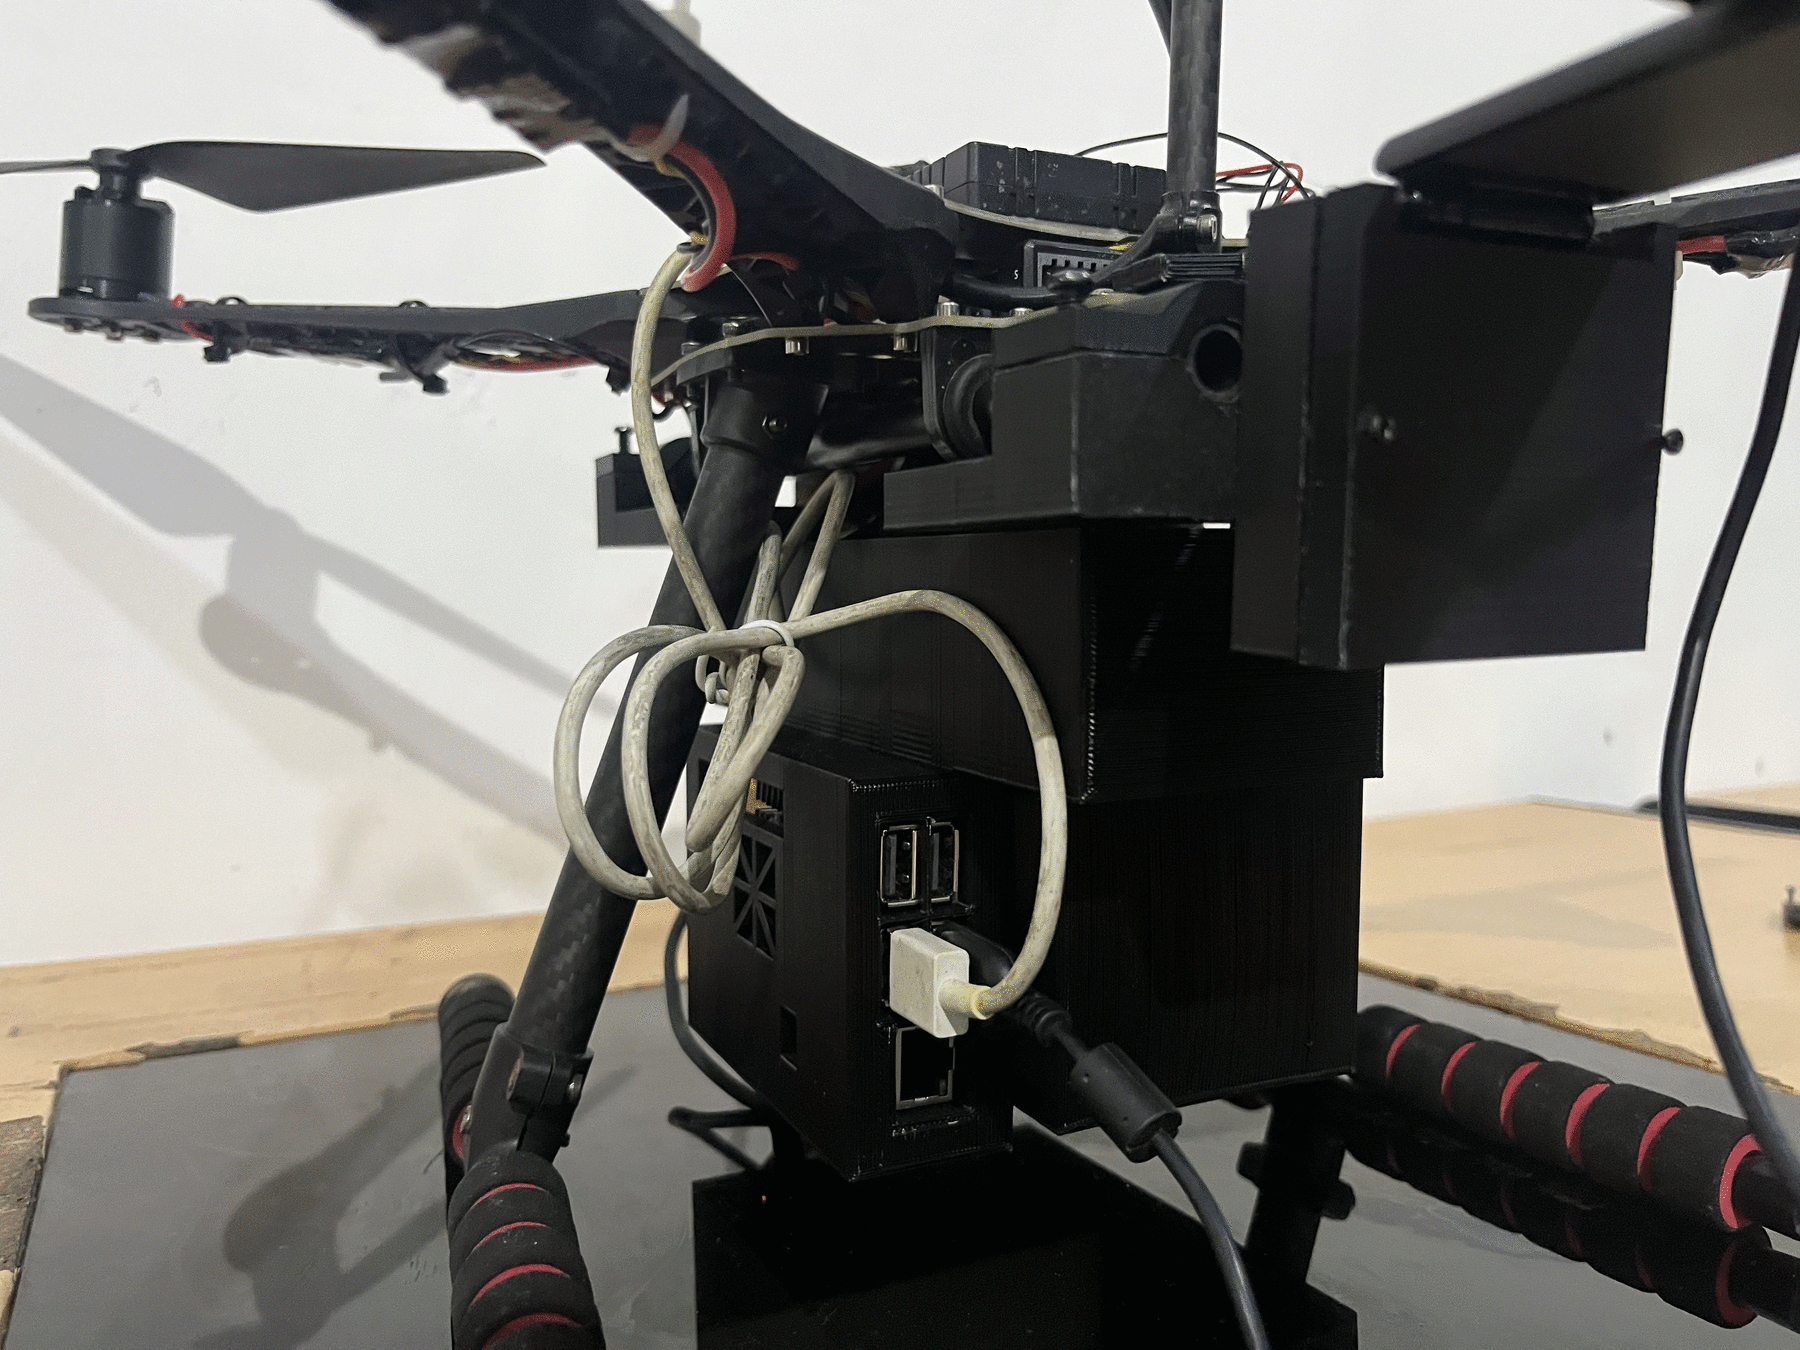
\includegraphics[width=0.7\textwidth]{bab3/serial_px4_rpi5_depan} 
			\caption{Tampak Depan (Desain Awal)}
		\end{subfigure}
		\hfill
		\begin{subfigure}[b]{0.45\textwidth}
			\centering
			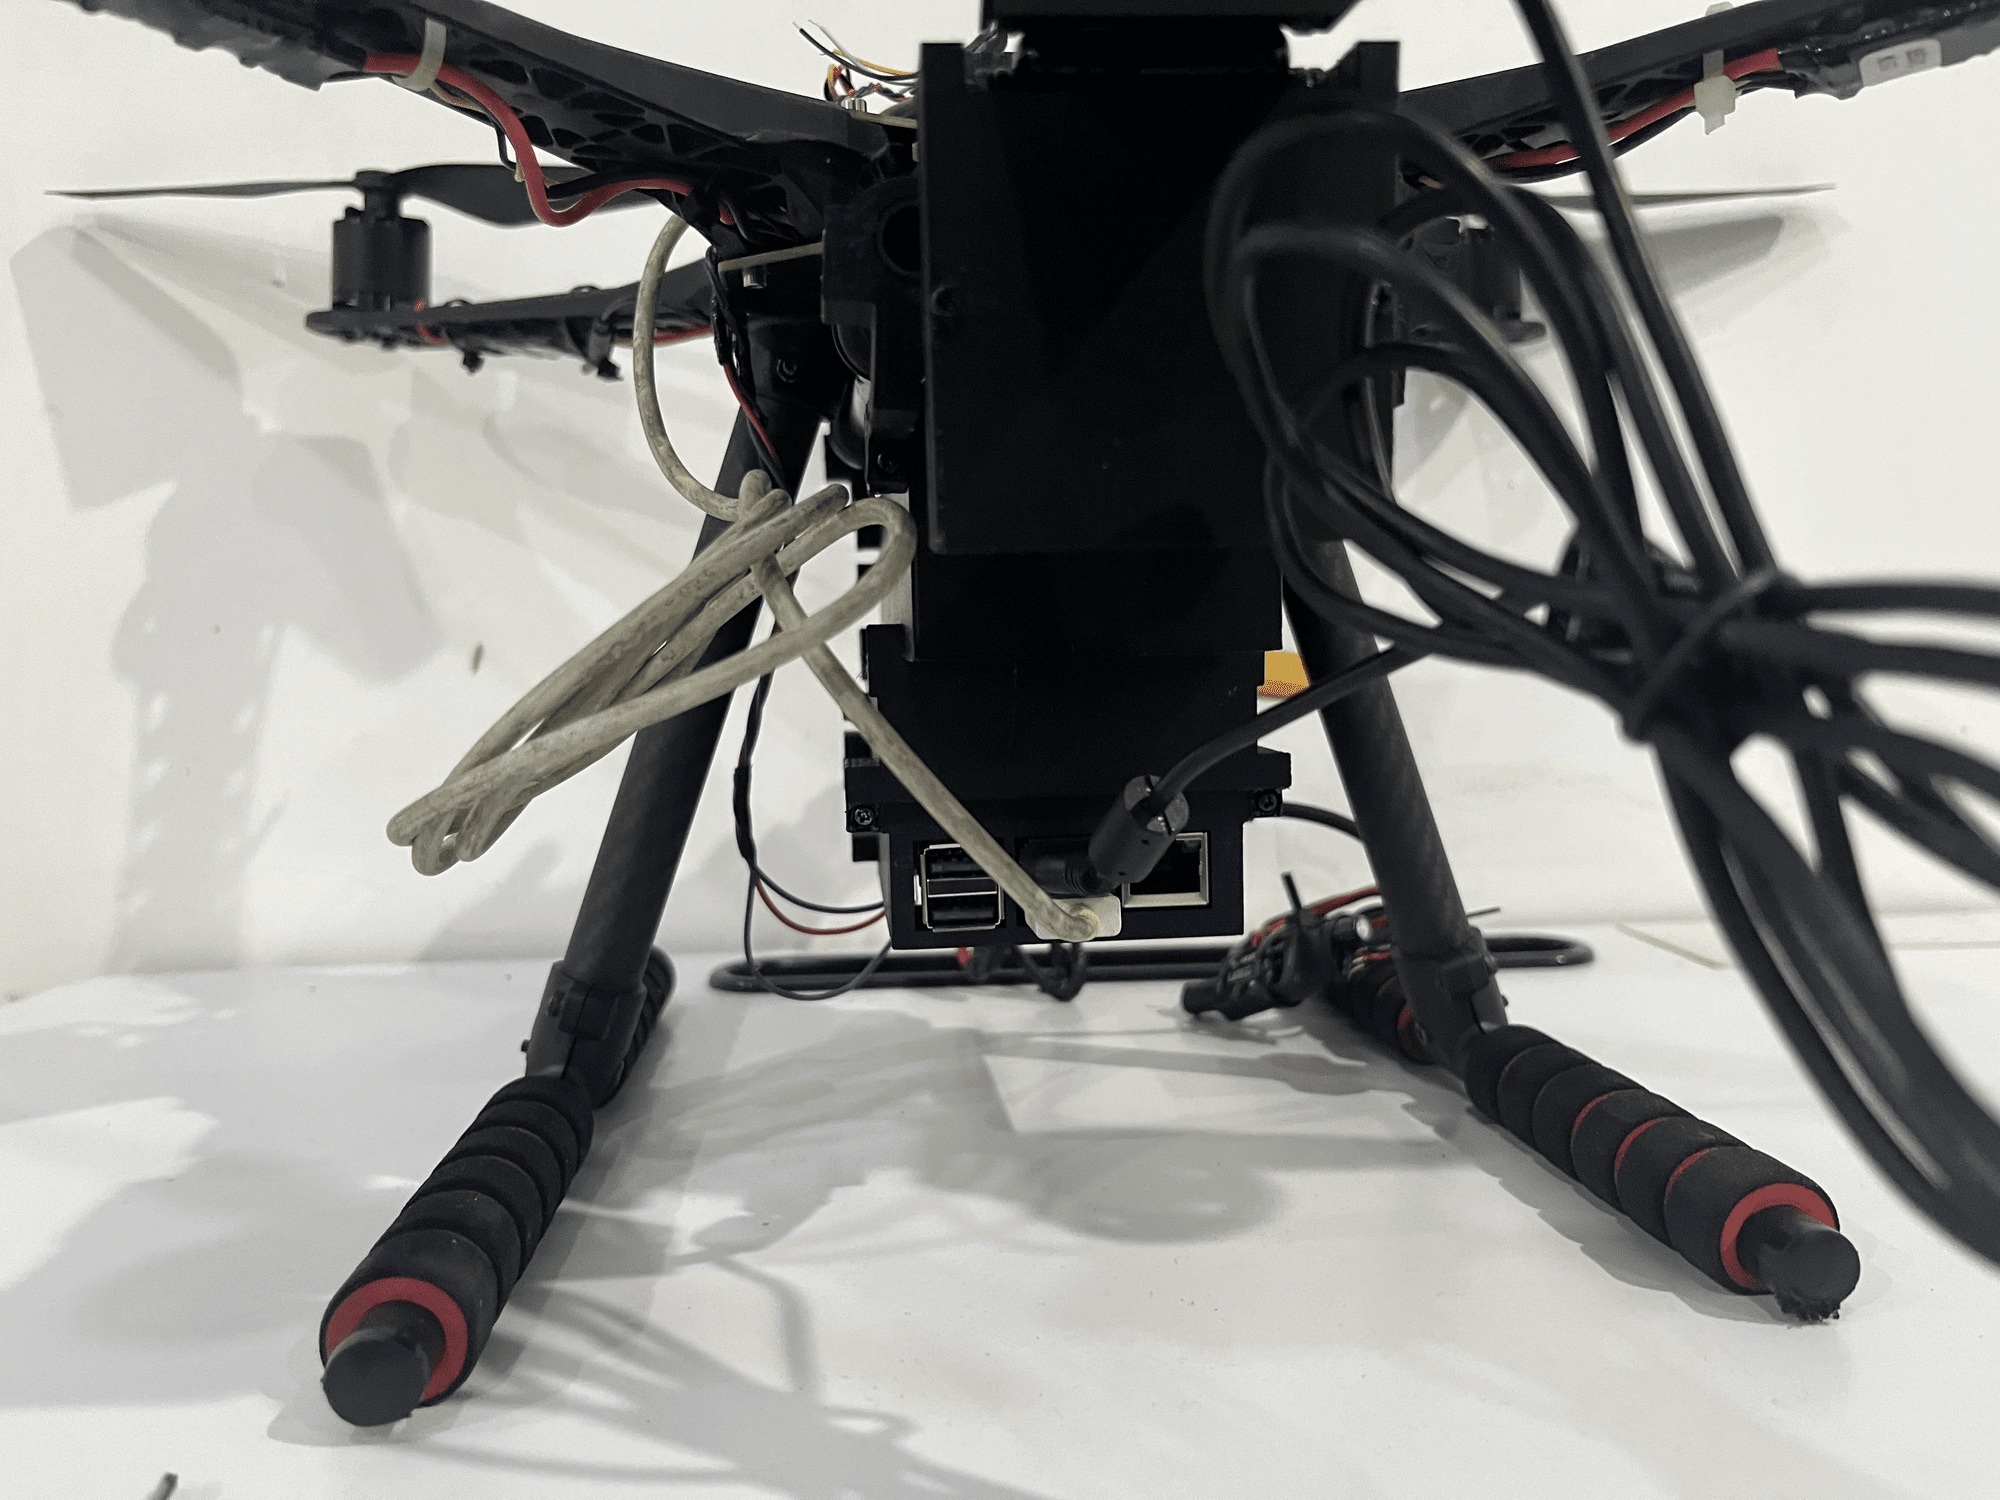
\includegraphics[width=0.7\textwidth]{bab3/usb_px4_rpi5_depan_desainbaru} 
			\caption{Tampak Depan (Desain Baru)}
		\end{subfigure}
		
		\vspace{0.5cm}
		
		\begin{subfigure}[b]{0.45\textwidth}
			\centering
			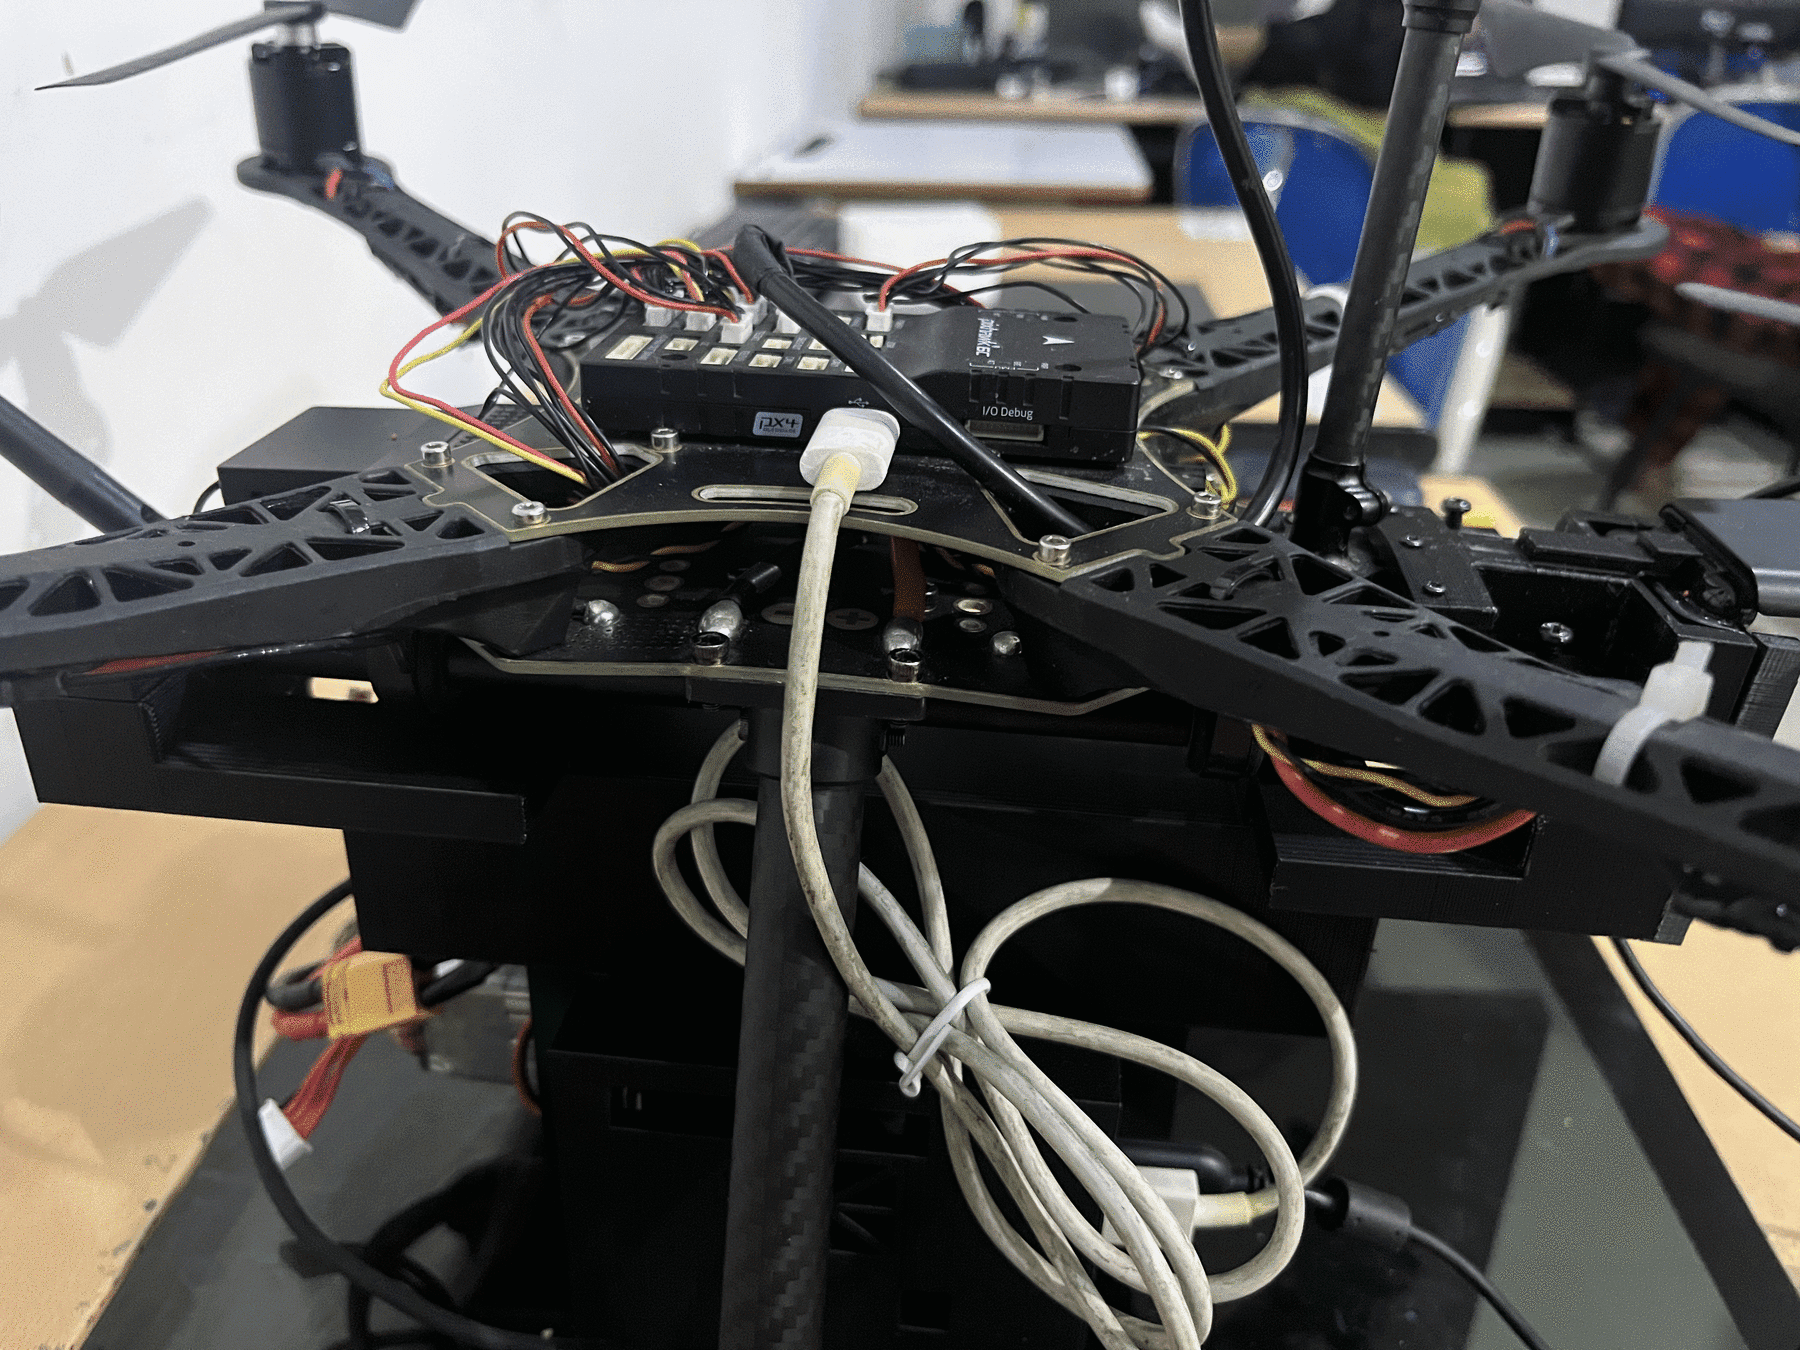
\includegraphics[width=0.9\linewidth]{bab3/serial_px4_rpi5_samping}
			\caption{Tampak Samping (Desain Awal)}
		\end{subfigure}
		\hfill
		\begin{subfigure}[b]{0.45\textwidth}
			\centering
			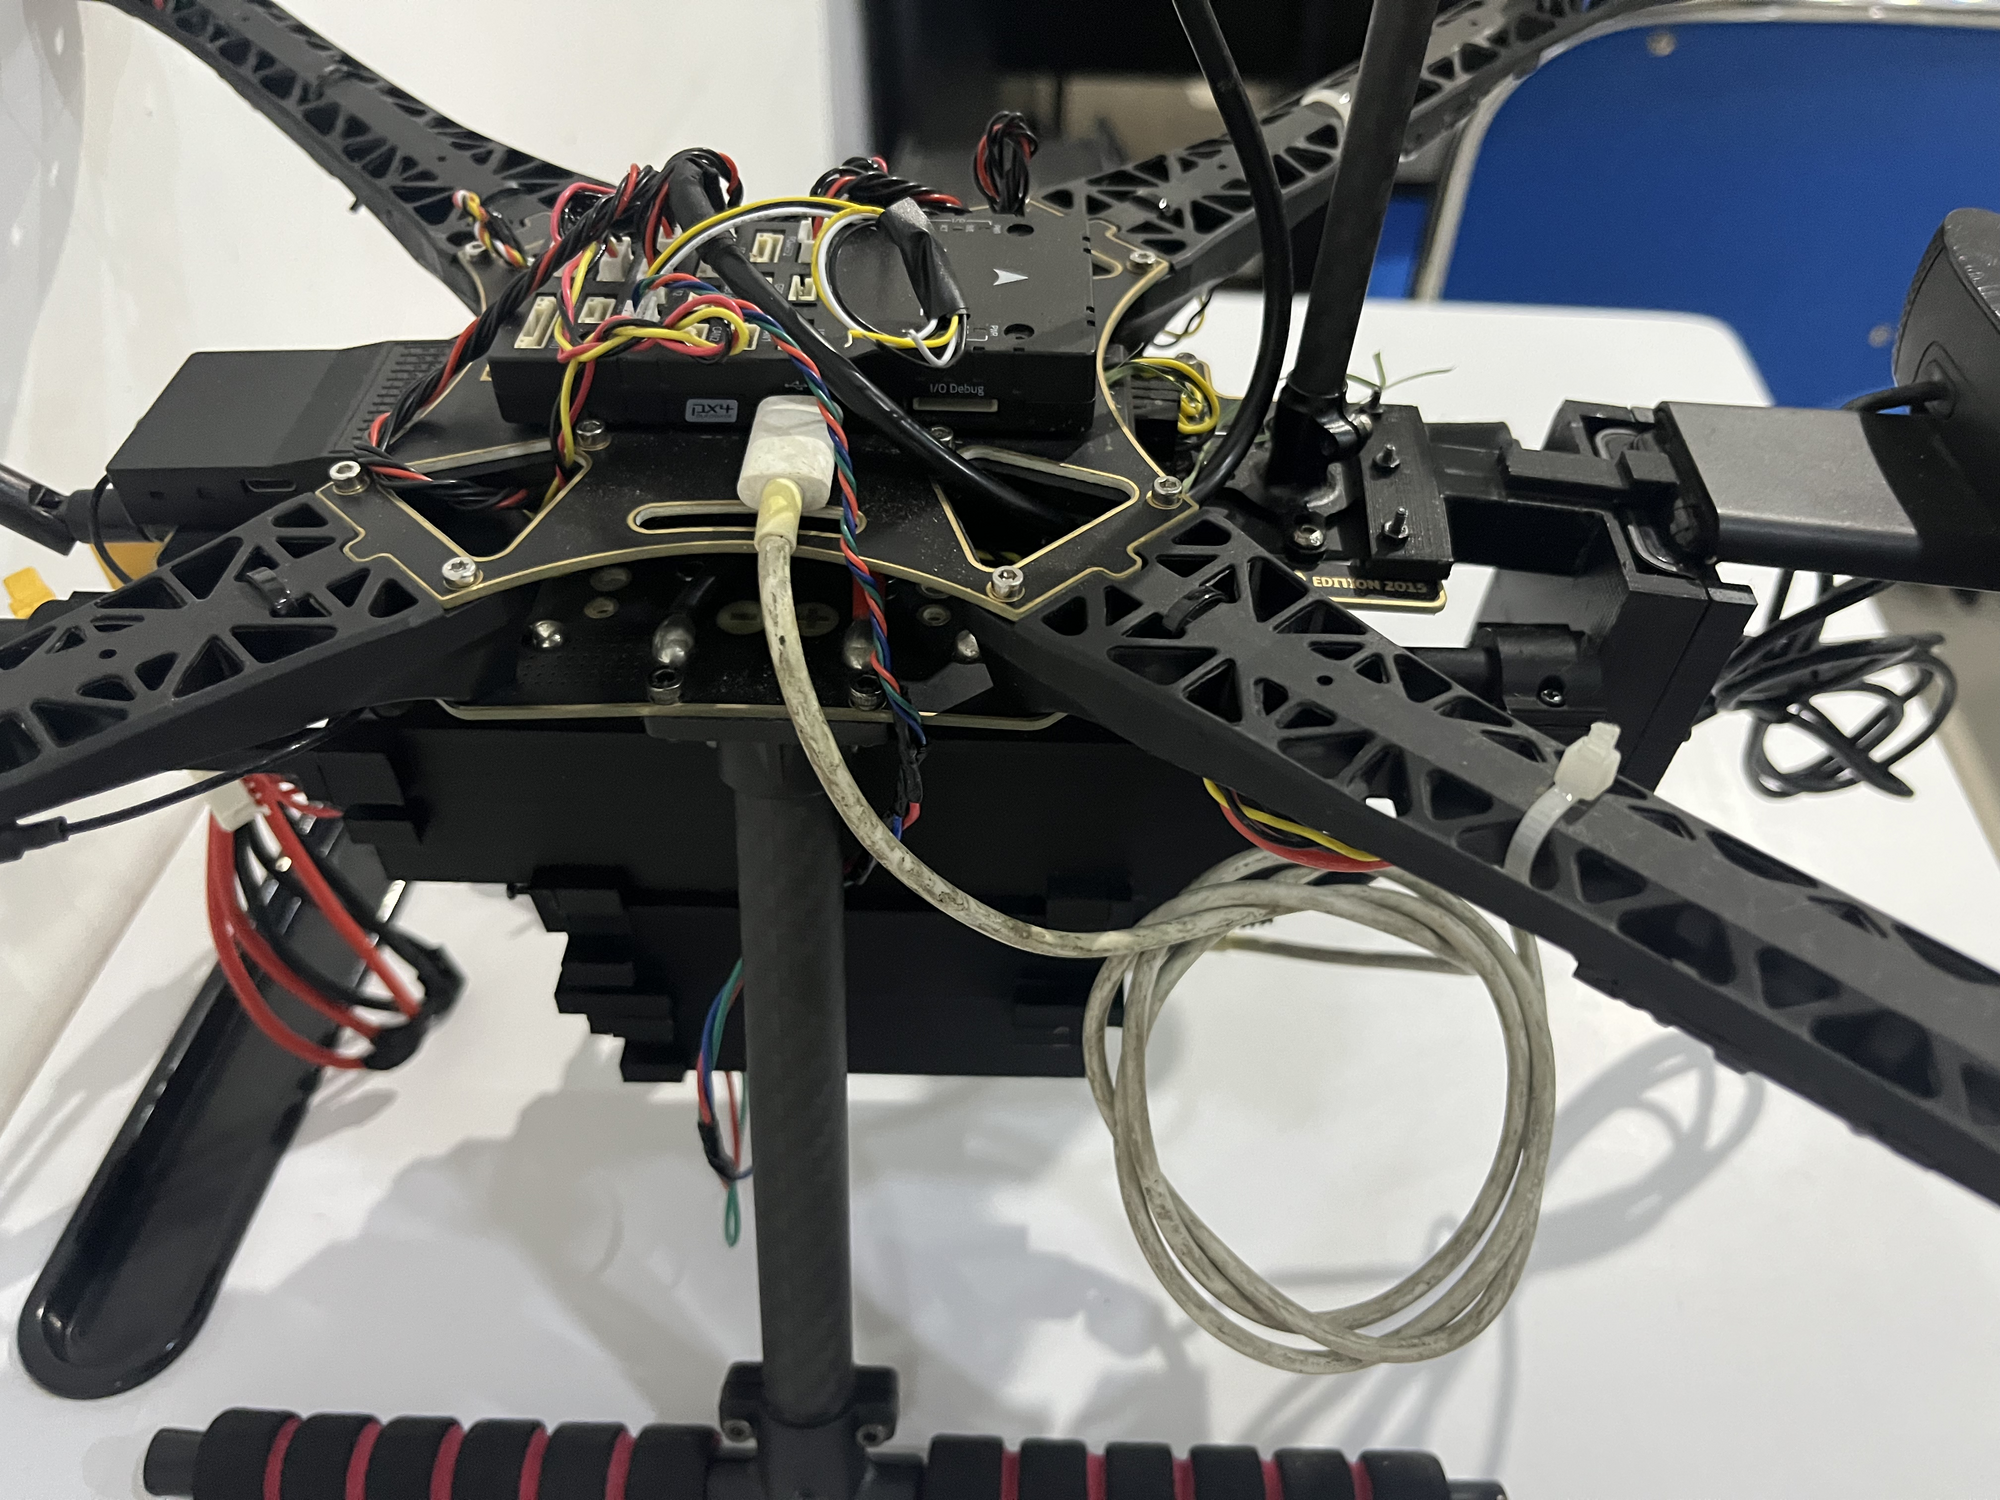
\includegraphics[width=0.9\linewidth]{bab3/usb_px4_rpi5_samping_desainbaru}
			\caption{Tampak Samping (Desain Baru)}
		\end{subfigure}
		\caption{Jalur komunikasi serial USB antara Pixhawk dan Raspberry Pi 5}
		\label{fig:serial-px4-rpi5-depan}
	\end{figure}

	\begin{figure}[H]
		\centering
		\begin{subfigure}[b]{0.45\textwidth}
			\centering
			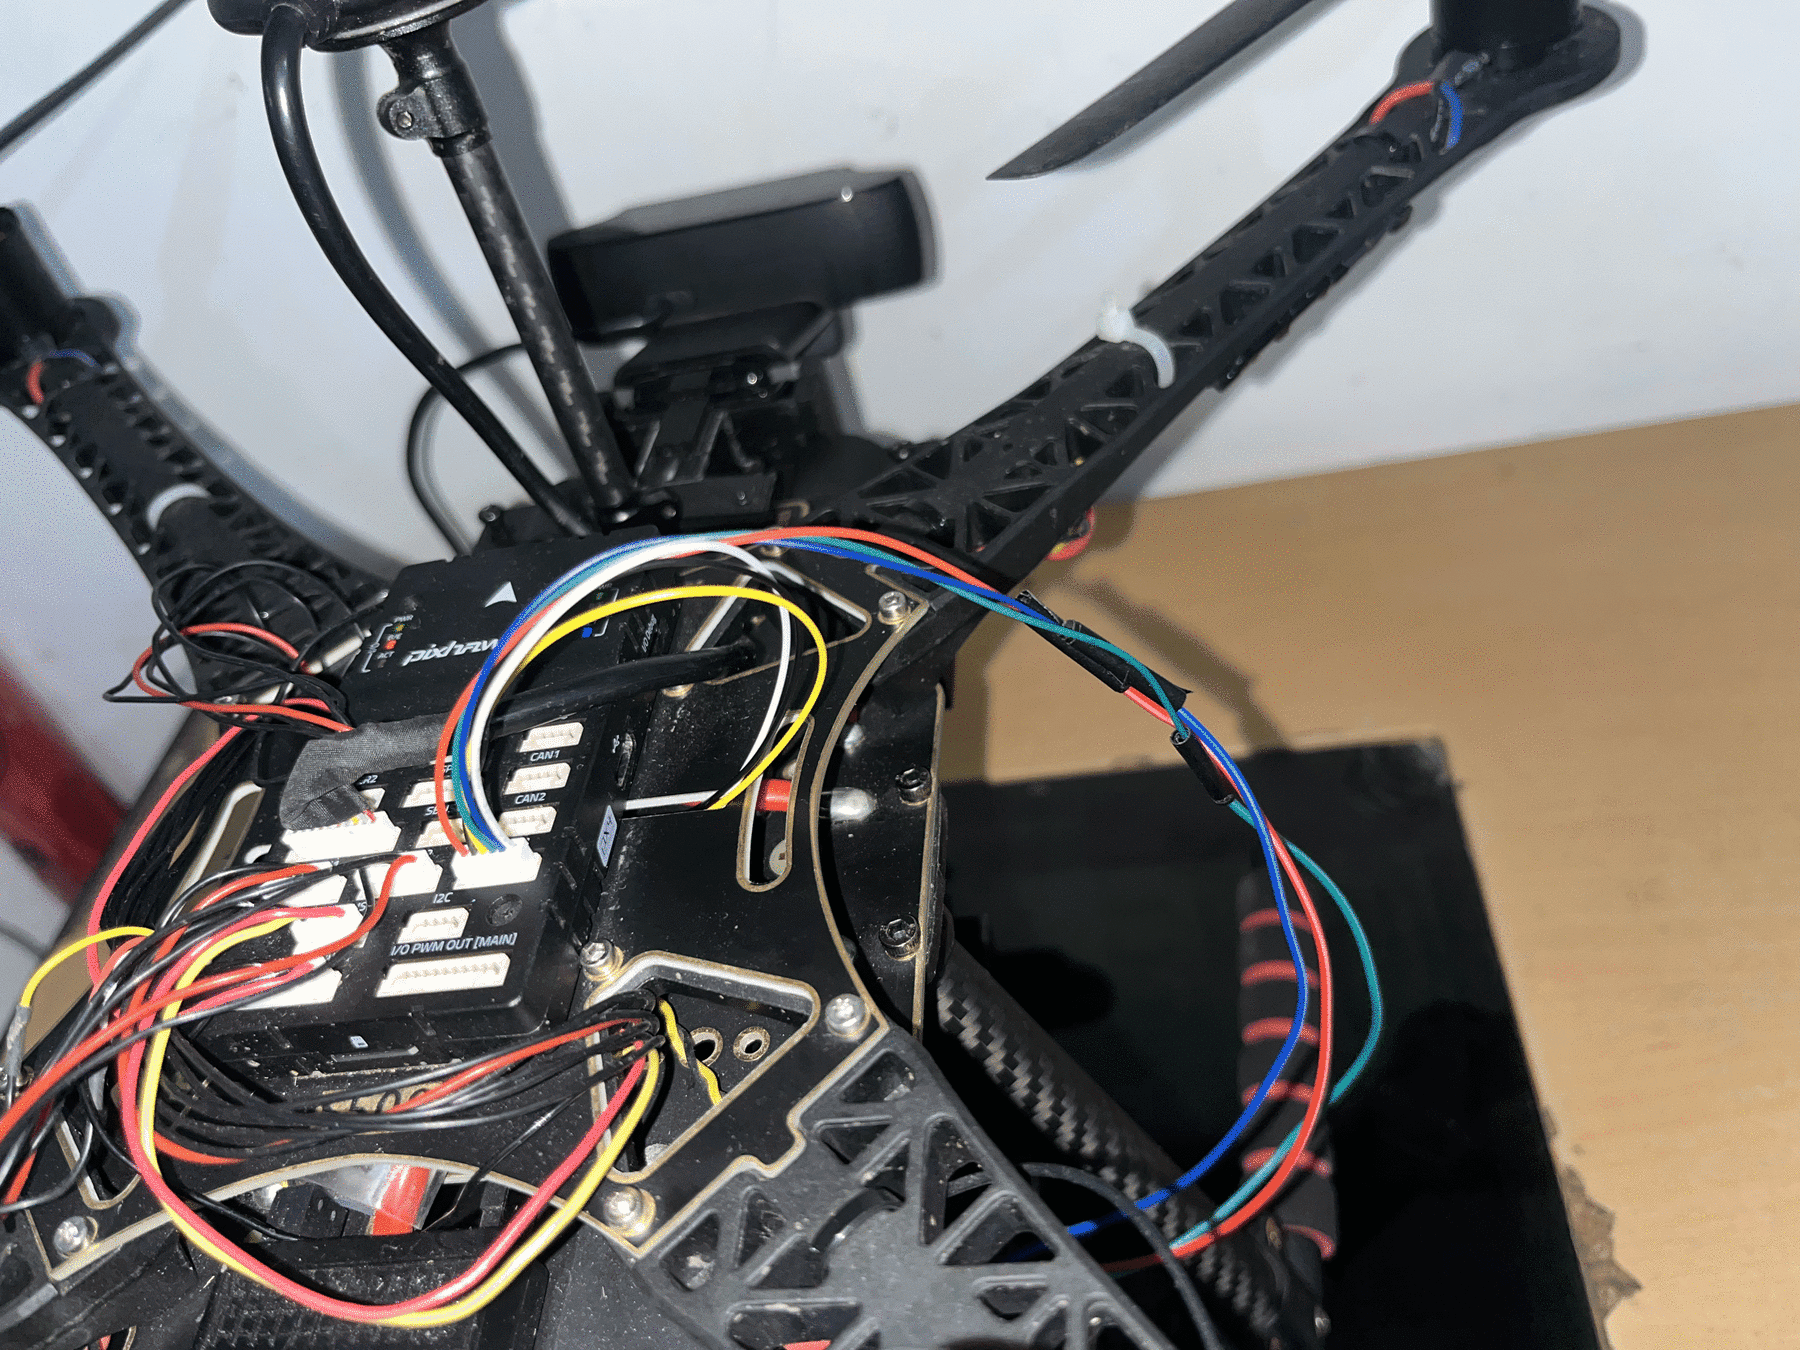
\includegraphics[width=0.7\textwidth]{bab3/serial_uart_px4_rpi5_depan} 
			\caption{Tampak Depan (Desain Awal)}
		\end{subfigure}
		\hfill
		\begin{subfigure}[b]{0.45\textwidth}
			\centering
			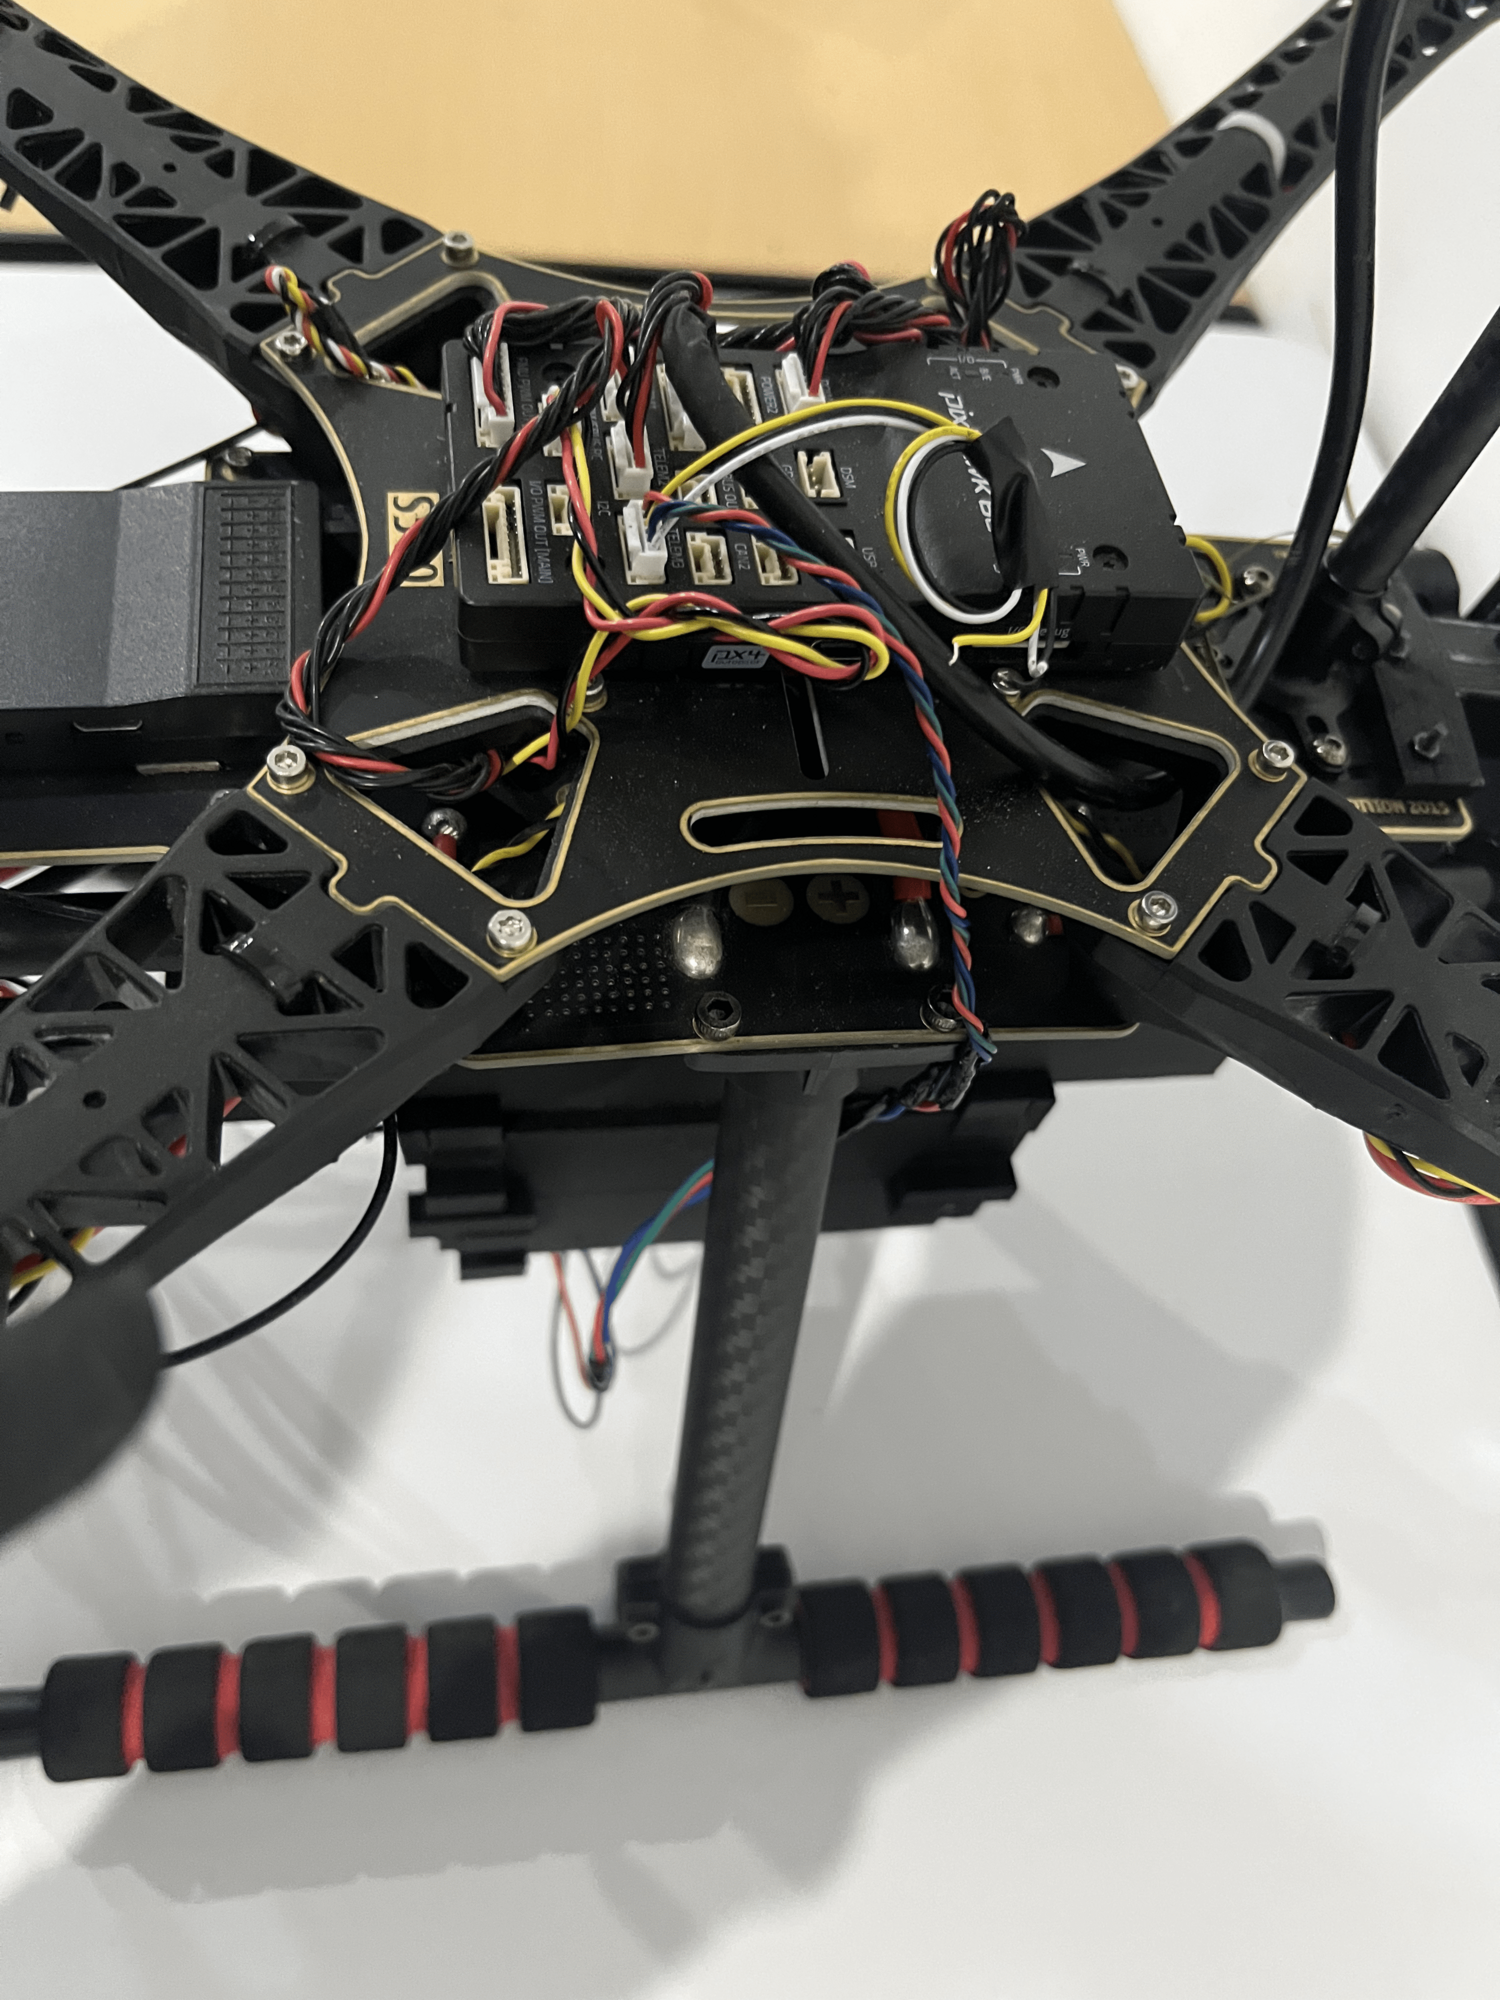
\includegraphics[width=0.7\textwidth]{bab3/serial_uart_px4_rpi5_depan_desainbaru} 
			\caption{Tampak Depan (Desain Baru)}
		\end{subfigure}
		
		\vspace{0.5cm}
		
		\begin{subfigure}[b]{0.45\textwidth}
			\centering        
			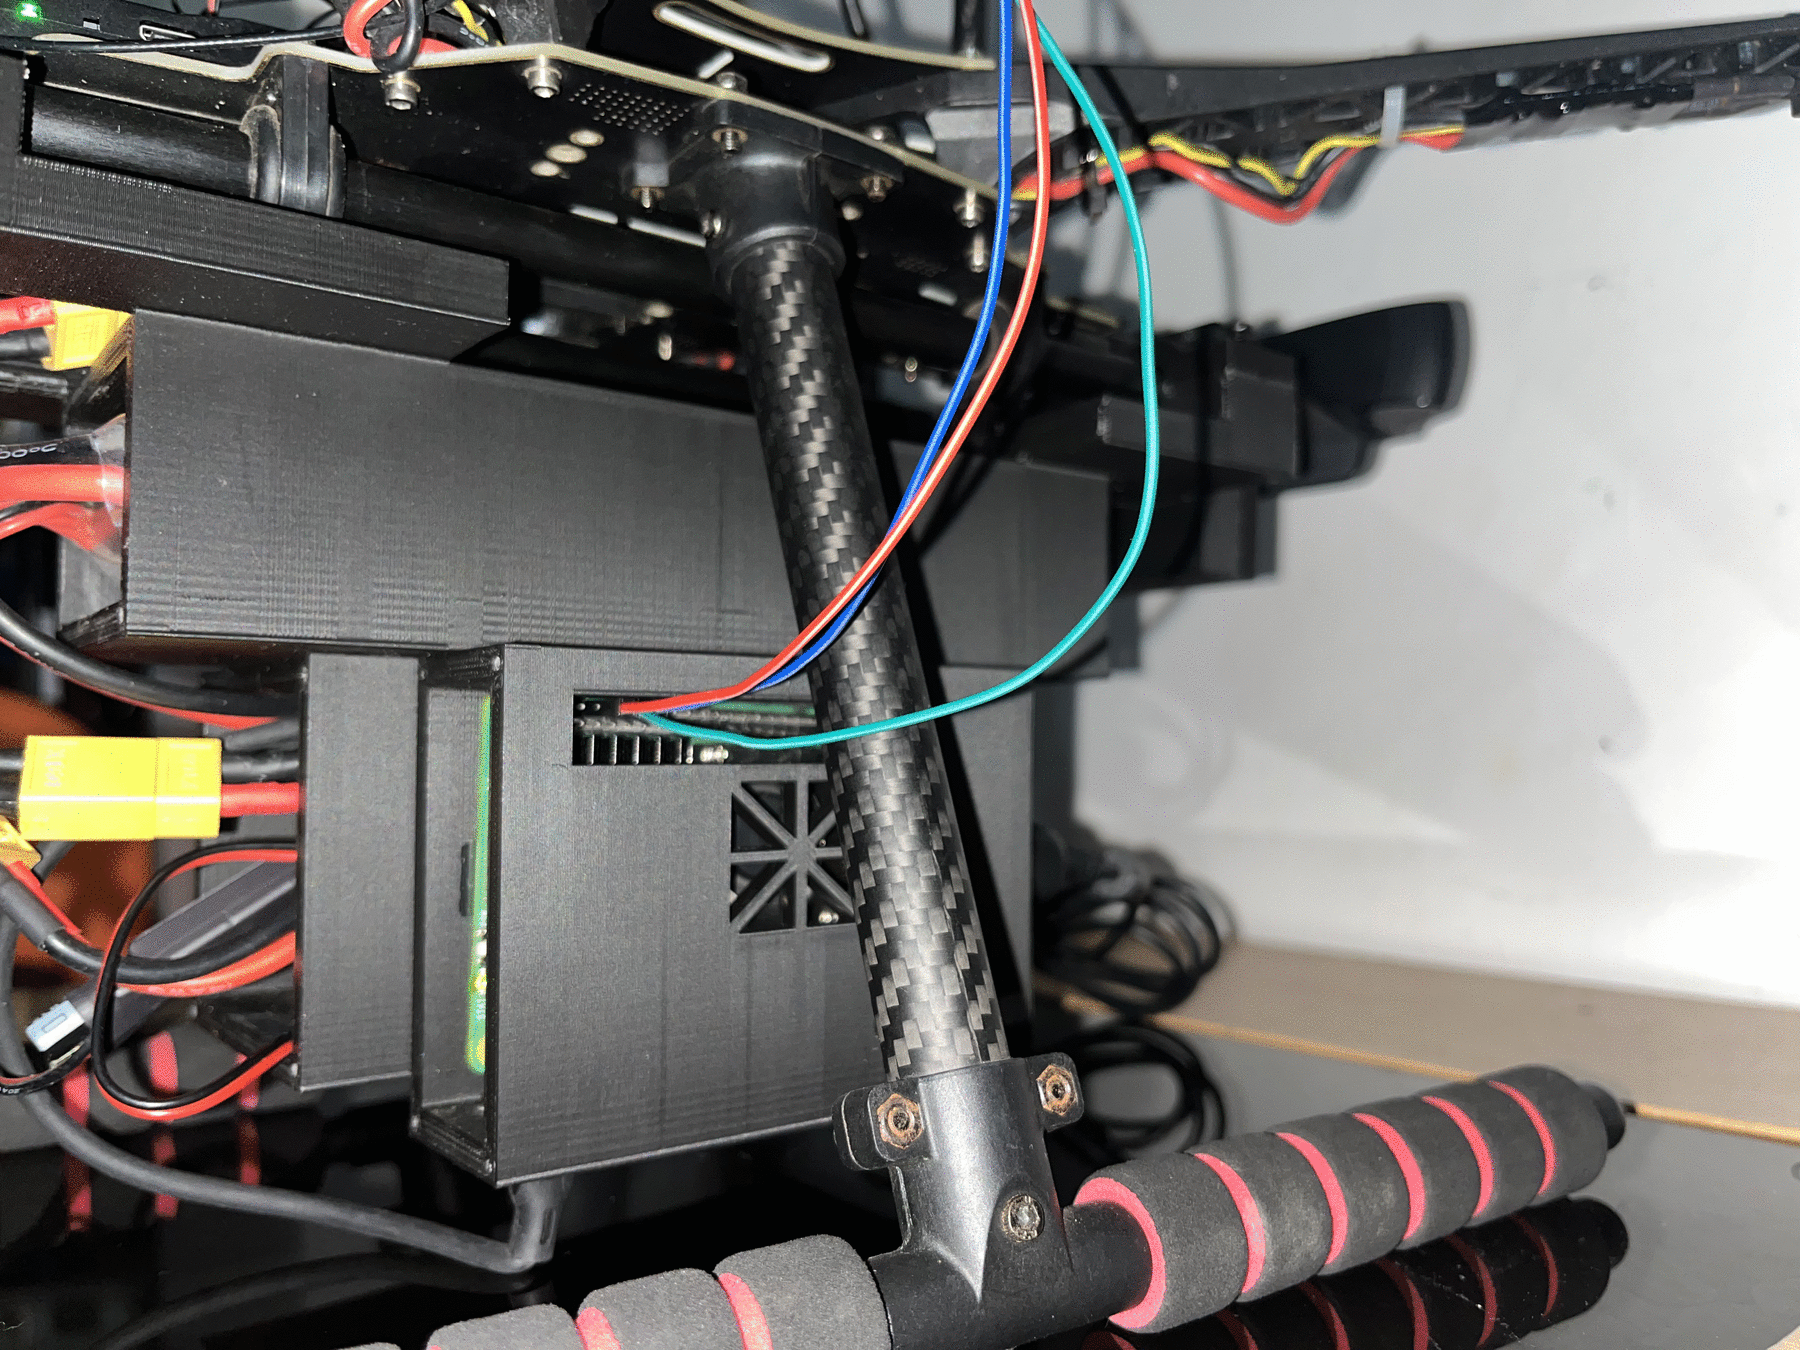
\includegraphics[width=0.9\linewidth]{bab3/serial_uart_px4_rpi5_samping}
			\caption{Tampak Samping (Desain Awal)}
		\end{subfigure}
		\hfill
		\begin{subfigure}[b]{0.45\textwidth}
			\centering        
			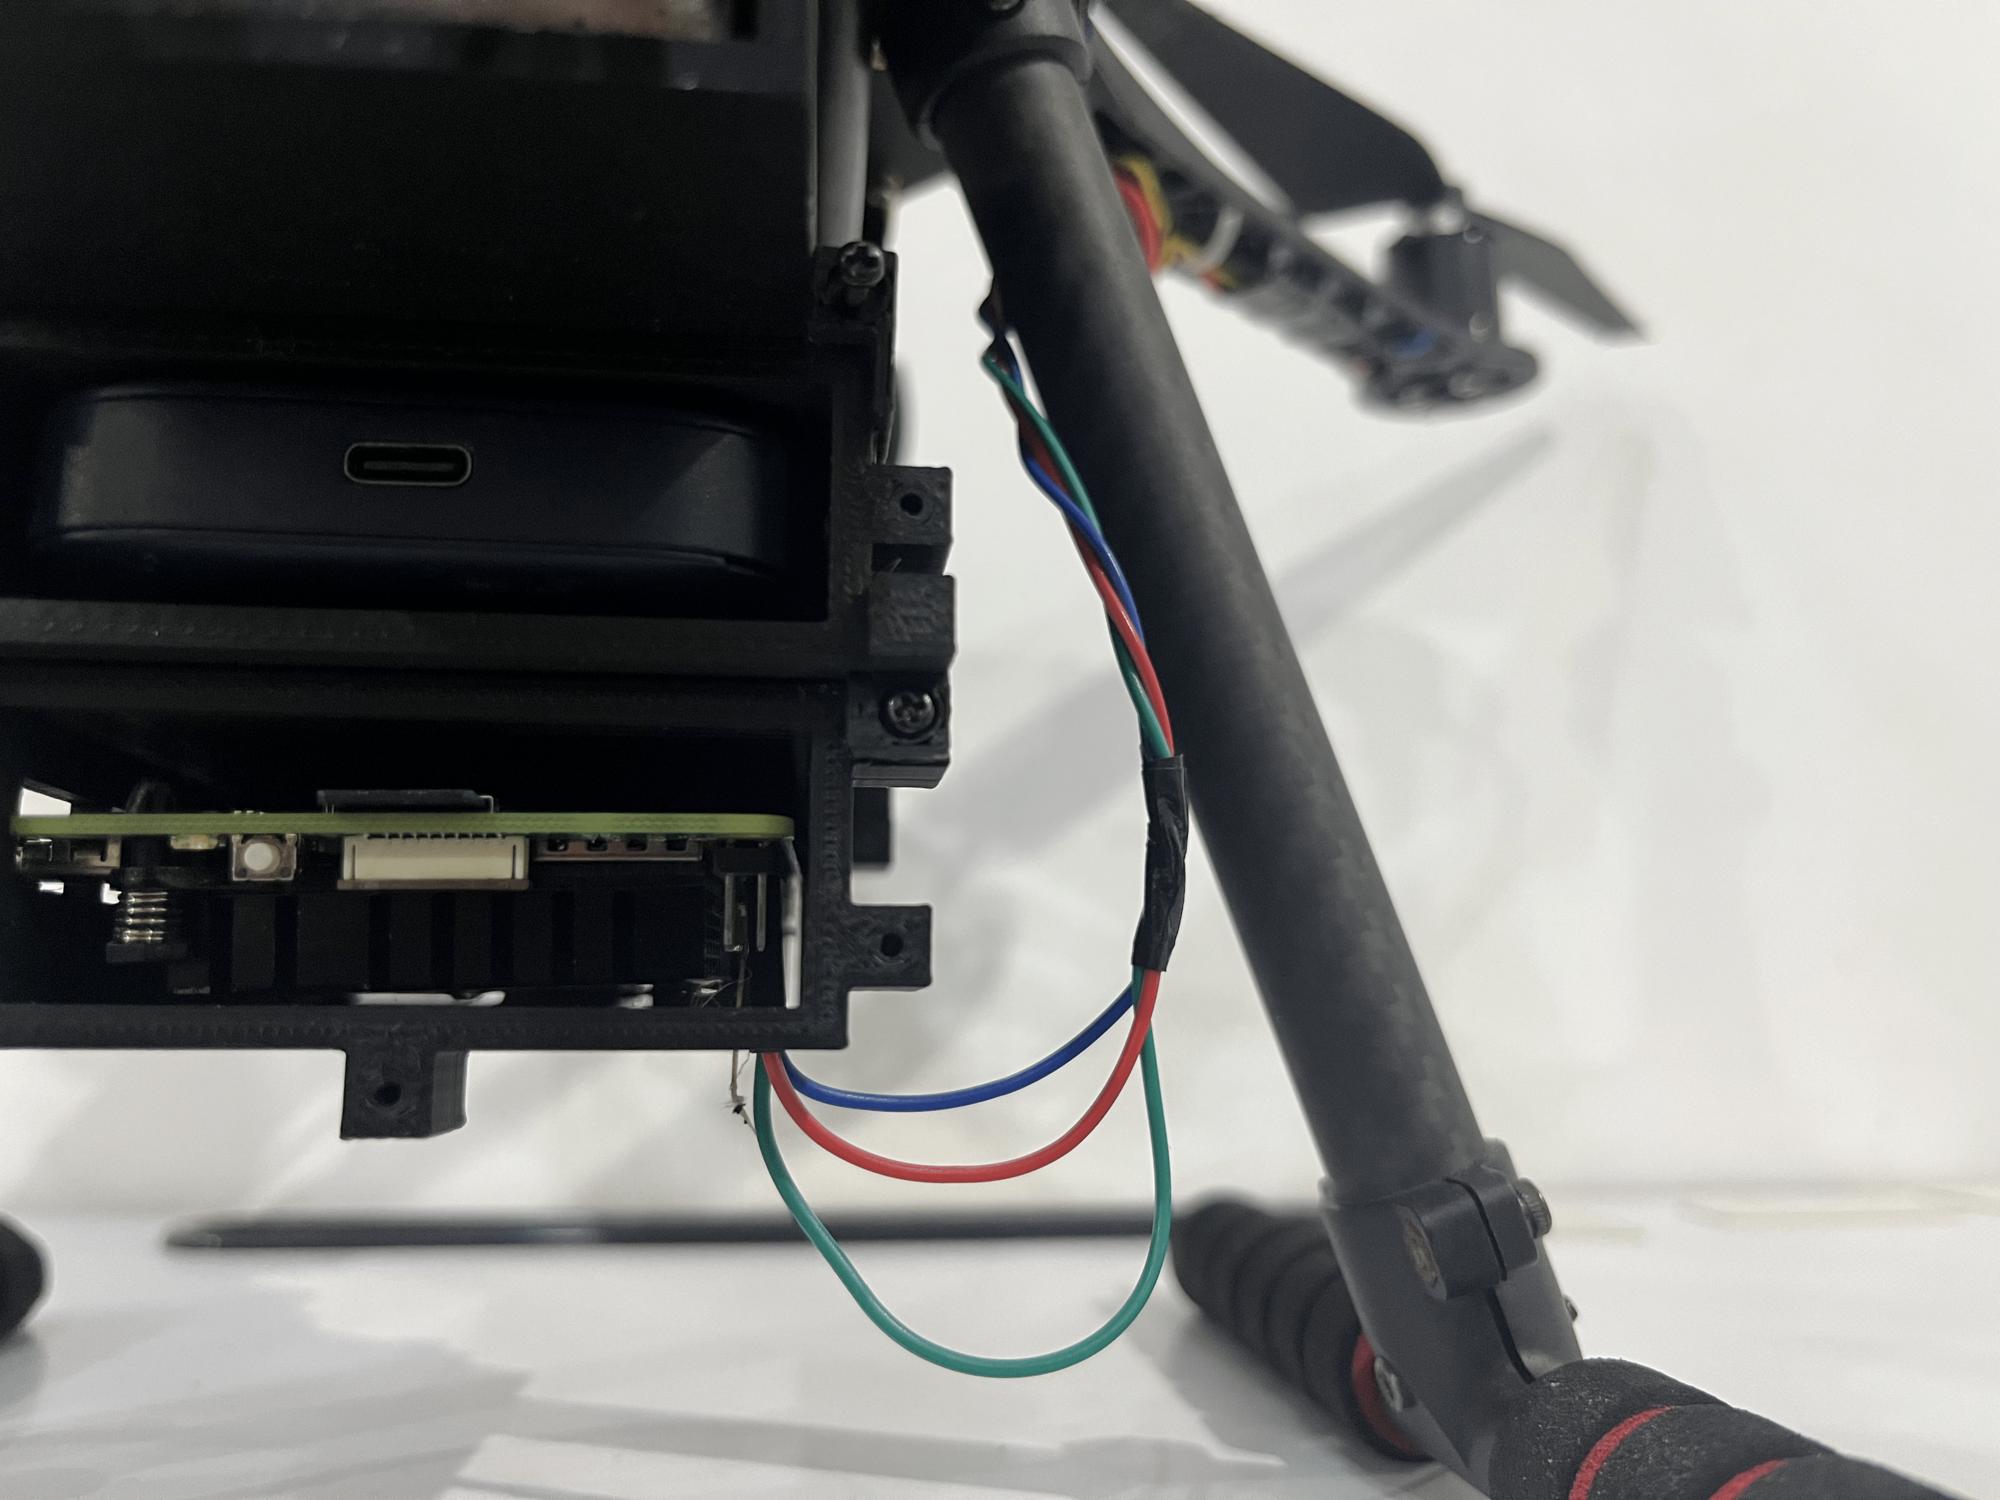
\includegraphics[width=0.9\linewidth]{bab3/serial_uart_px4_rpi5_samping_desainbaru}
			\caption{Tampak Samping (Desain Baru)}
		\end{subfigure}
		\caption{Jalur komunikasi serial (UART) antara Pixhawk dan Raspberry Pi 5}
		\label{fig:serial-uart-px4-rpi5-depan}
	\end{figure}
	
	\item Realisasi Komponen Cetak 3D: Seluruh komponen hasil desain 3D (seperti dudukan utama kompartemen, \textit{retainer} baterai, dan casing pelindung) dicetak menggunakan material \textit{Polylactic Acid} (PLA). Berikut adalah hasil realisasi fisik dari masing-masing komponen cetak 3D sebelum dirakit:
	\begin{enumerate}[]
		\item Dudukan Utama Kompartemen (\textit{Main Base})\\
		\begin{figure}[H]
			\centering
			\begin{subfigure}[b]{0.3\textwidth}
				\centering
				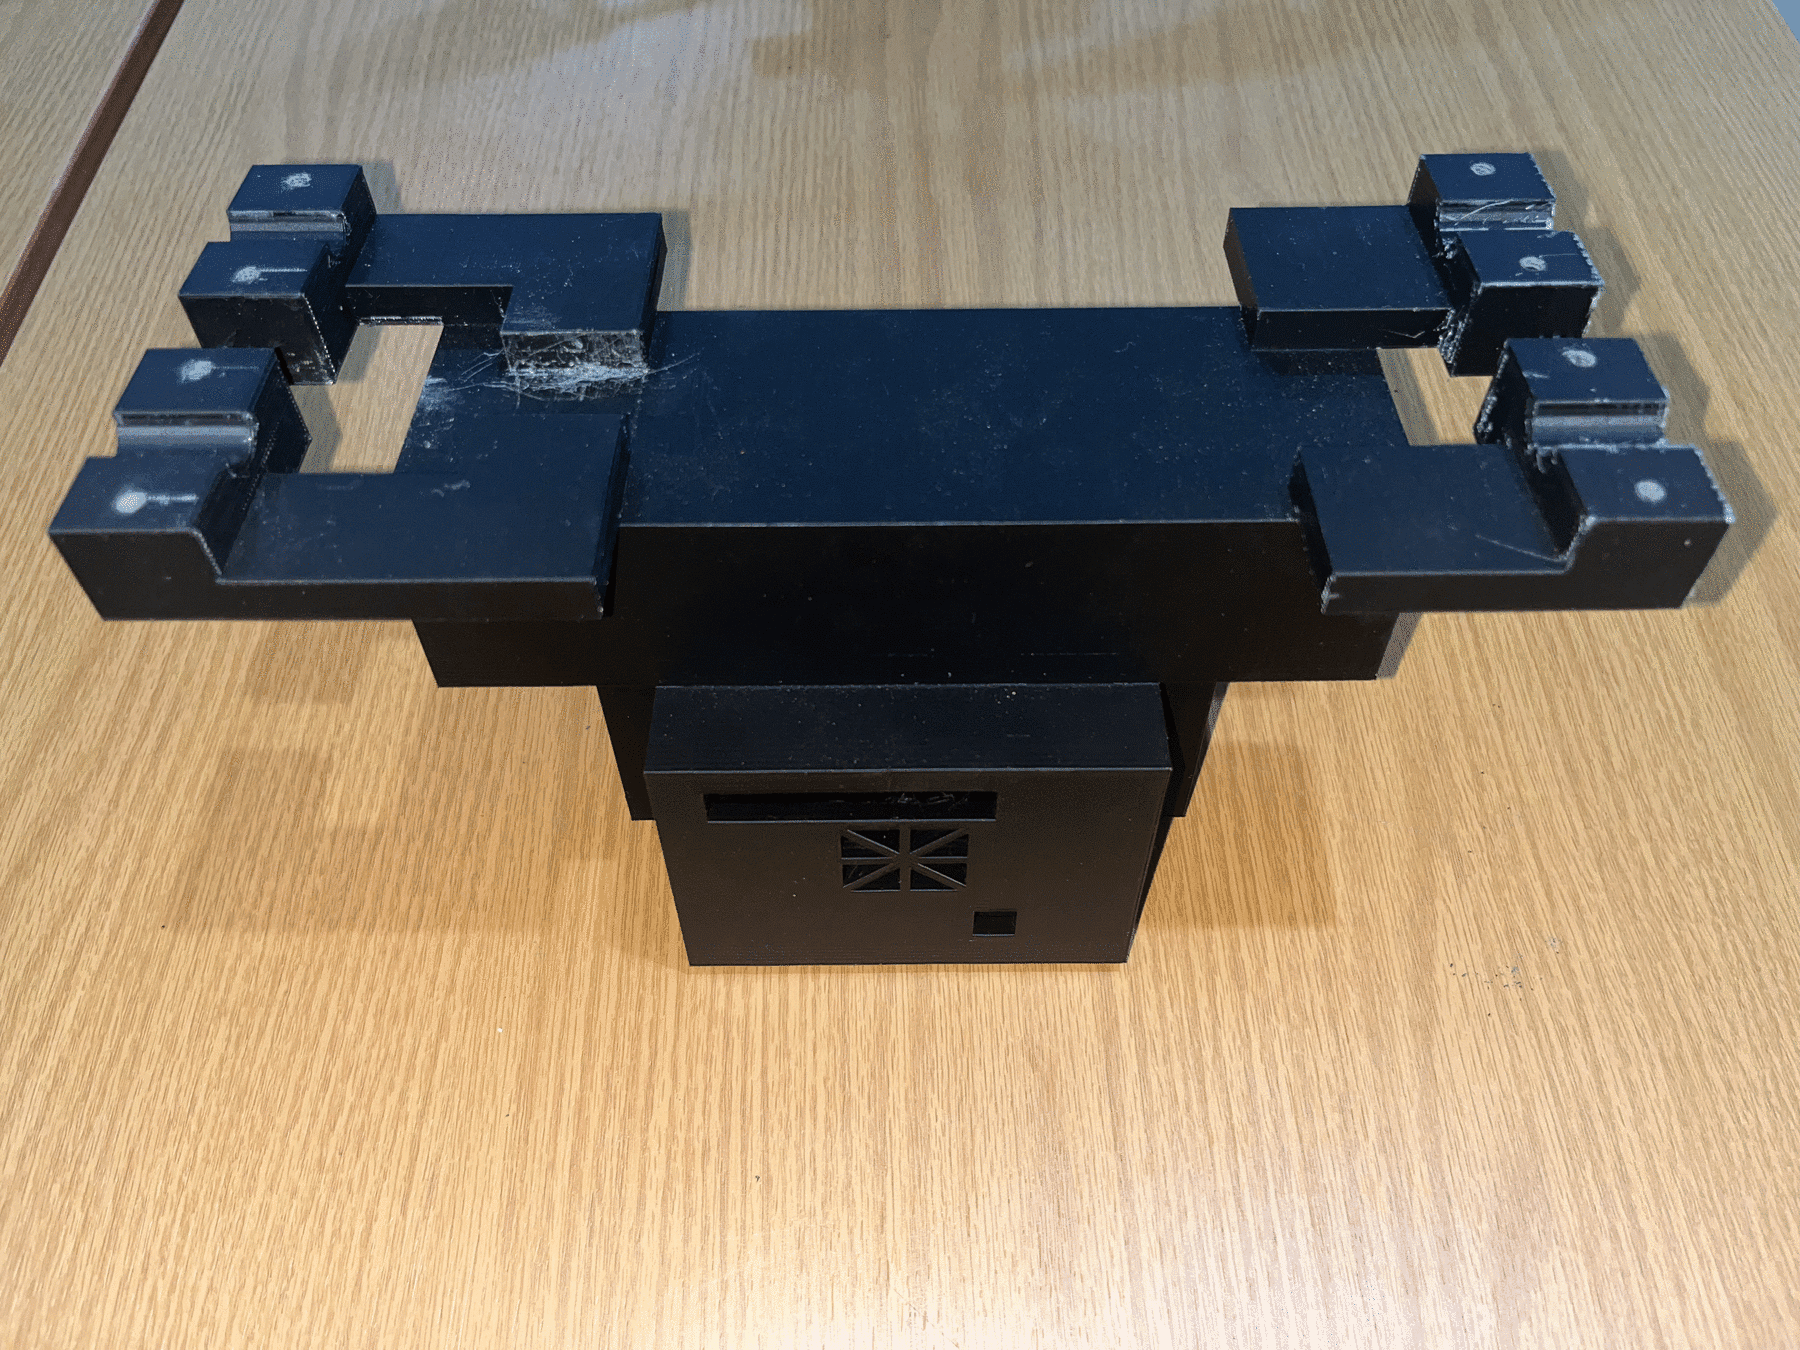
\includegraphics[width=0.7\linewidth]{bab3/dudukan_utama_kompartemen_real1}
				\caption{Hasil Realisasi Dudukan Utama Kompartemen Tampak Perspektif 1}
				\label{fig:dudukan-utama-kompartemen-real-1}
			\end{subfigure}
			\hfill
			\begin{subfigure}[b]{0.3\textwidth}
				\centering
				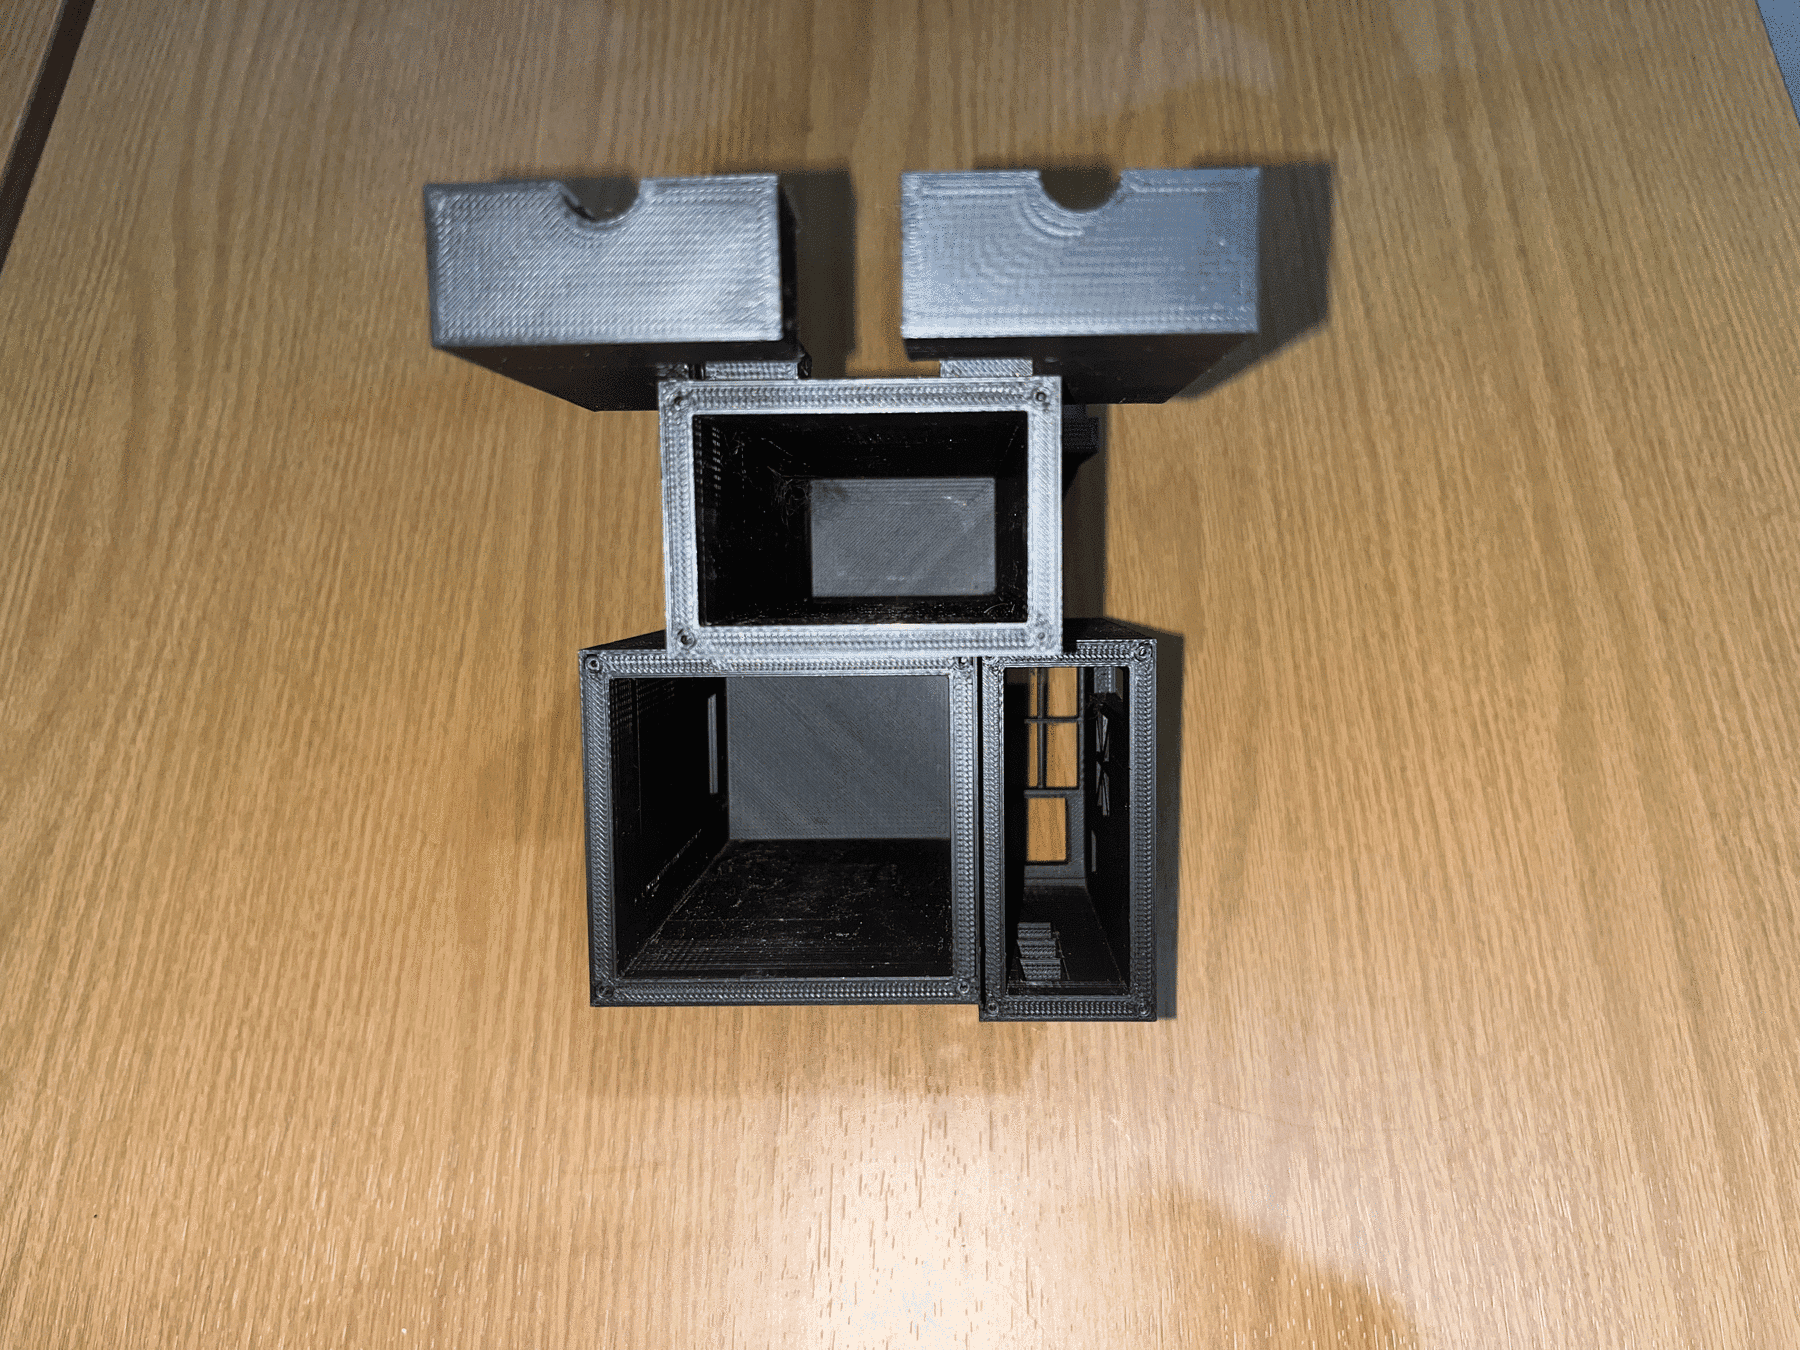
\includegraphics[width=0.7\linewidth]{bab3/dudukan_utama_kompartemen_real2}
				\caption{Hasil Realisasi Dudukan Utama Kompartemen Tampak Perspektif 2}
				\label{fig:dudukan-utama-kompartemen-real-2}
			\end{subfigure}
			\hfill
			\begin{subfigure}[b]{0.3\textwidth}
				\centering
				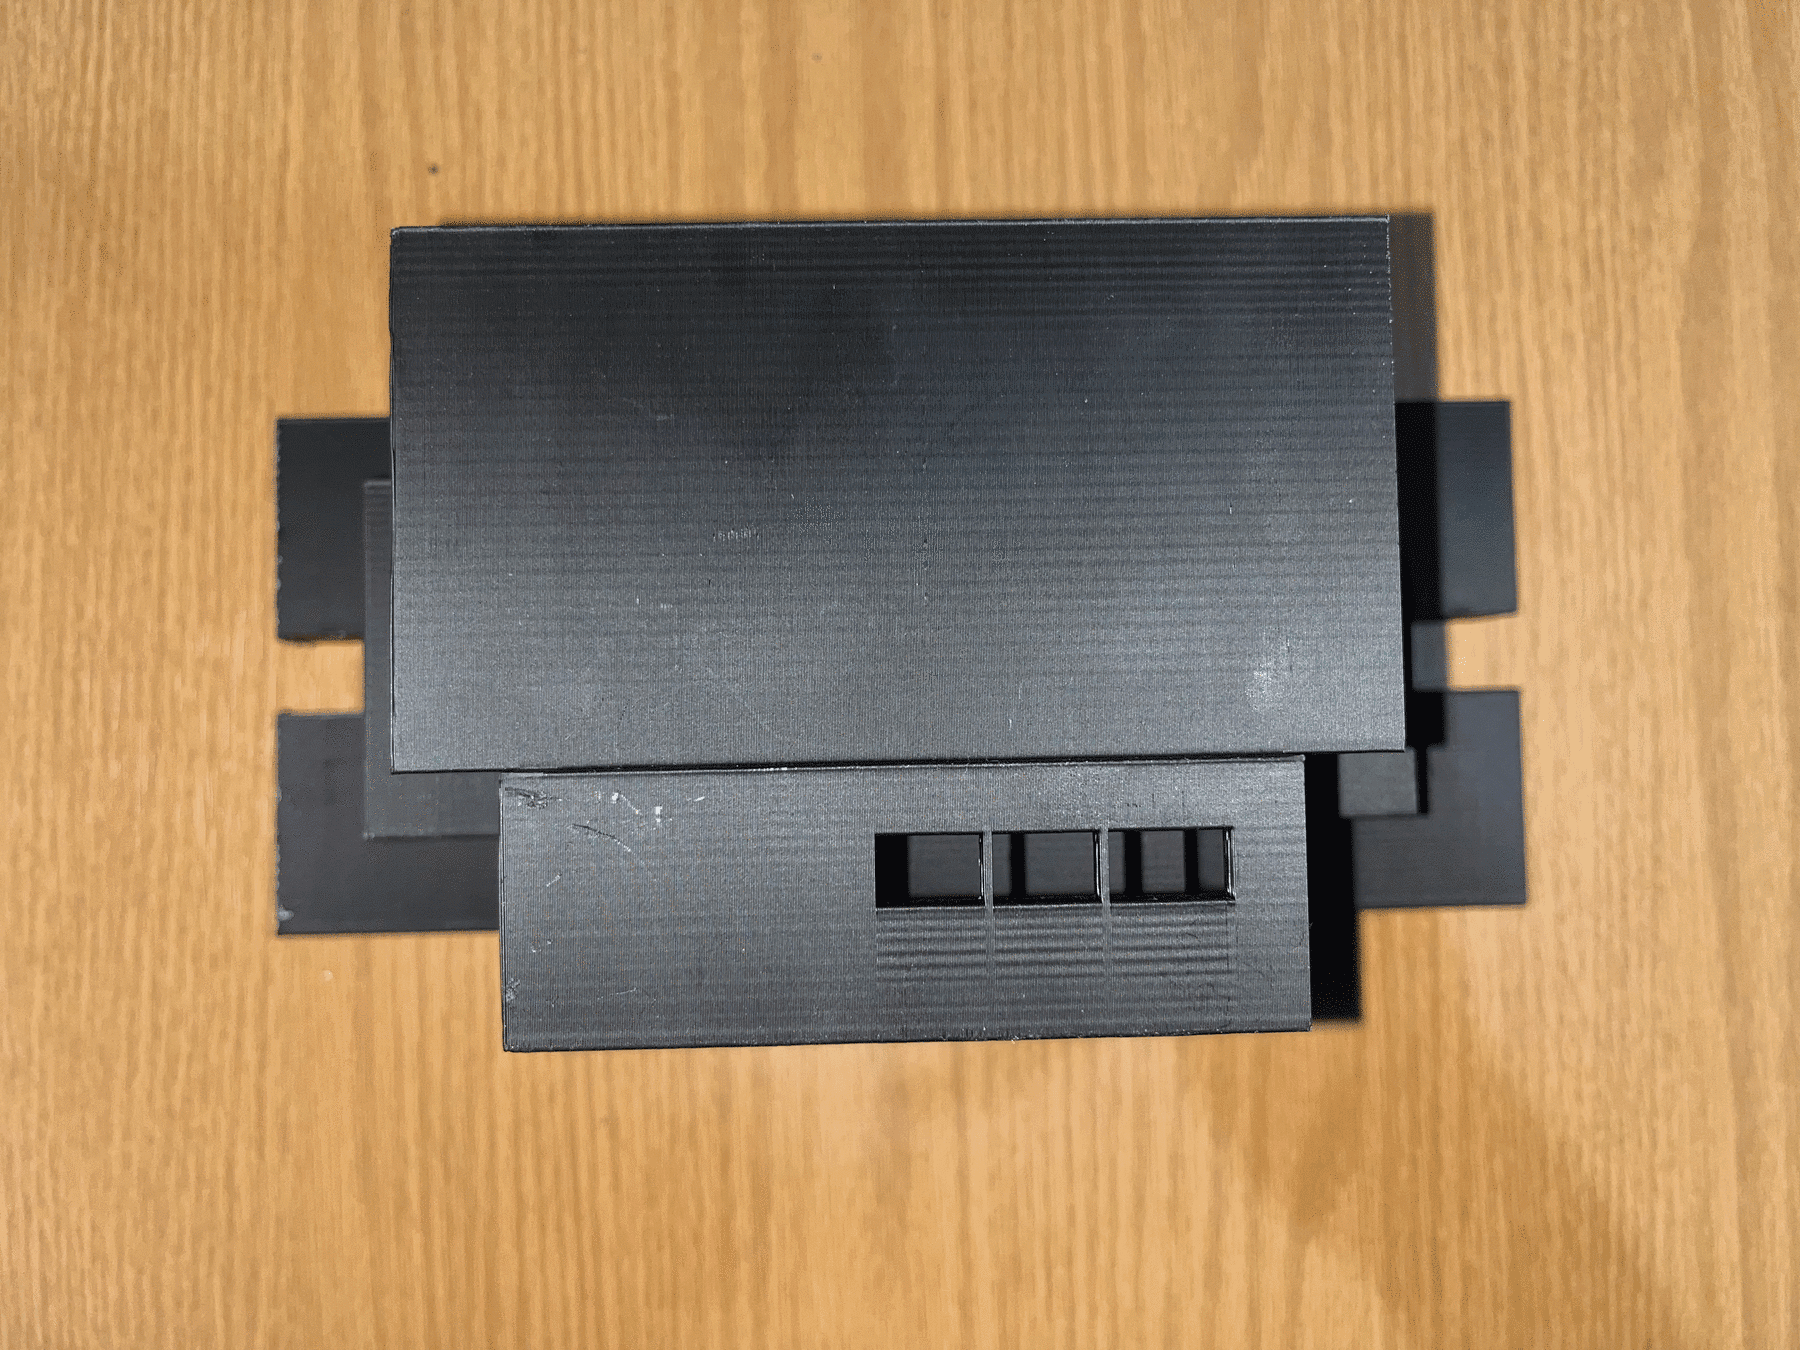
\includegraphics[width=0.7\linewidth]{bab3/dudukan_utama_kompartemen_real3}
				\caption{Hasil Realisasi Dudukan Utama Kompartemen Tampak Perspektif 3}
				\label{fig:dudukan-utama-kompartemen-real-3}
			\end{subfigure}
		\end{figure}
		\item Plat Pengikat Kompartemen (\textit{Top Plate})\\
		\begin{figure}[H]
			\centering
			\begin{subfigure}[b]{0.45\textwidth}
				\centering
				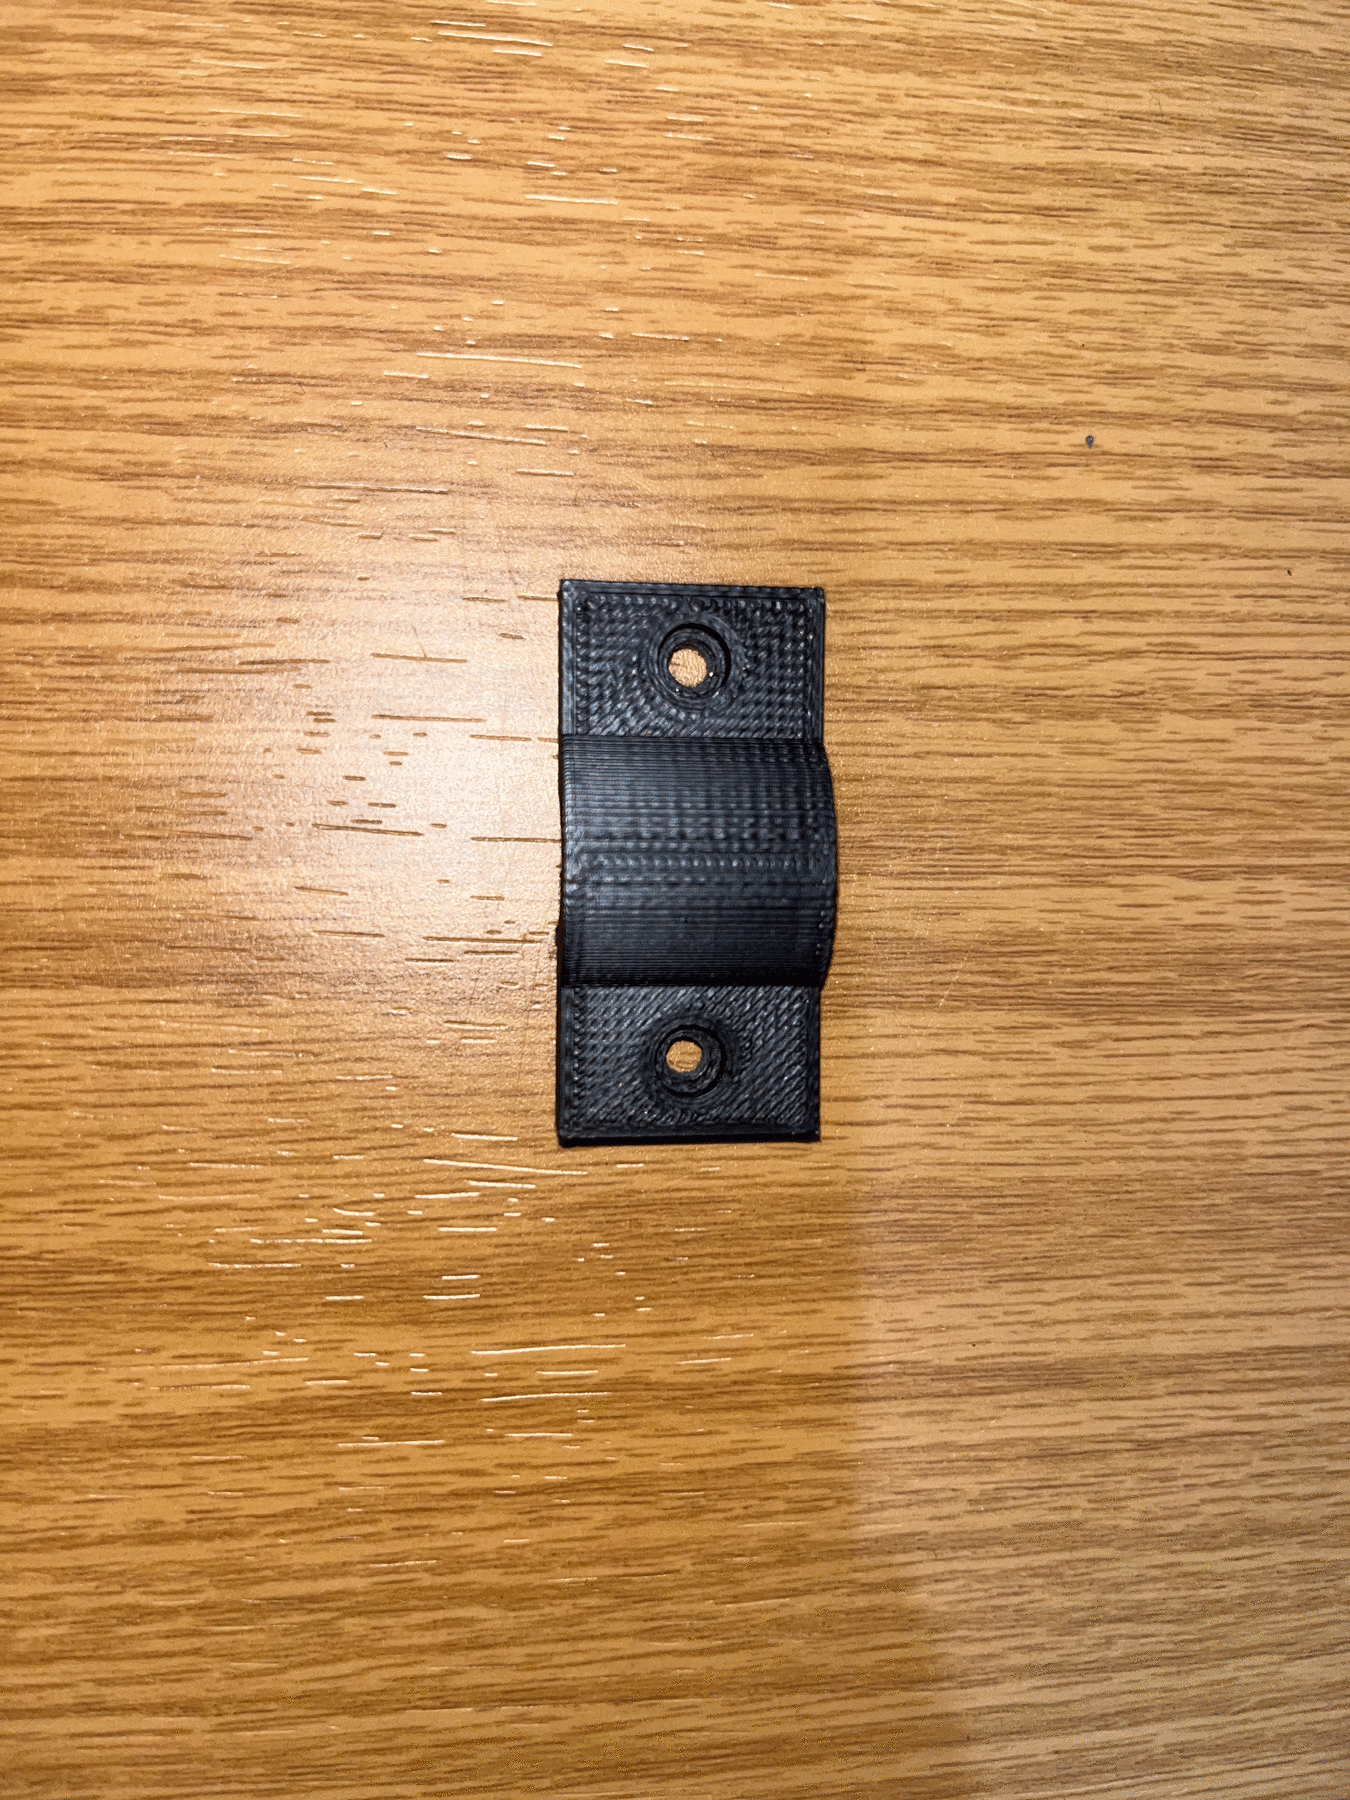
\includegraphics[width=0.7\linewidth]{bab3/top_plate_real1}
				\caption{Hasil Realisasi Plat Pengikat Kompartemen Tampak Perspektif 1}
				\label{fig:top-plate-real-1}
			\end{subfigure}
			\hfill
			\begin{subfigure}[b]{0.45\textwidth}
				\centering
				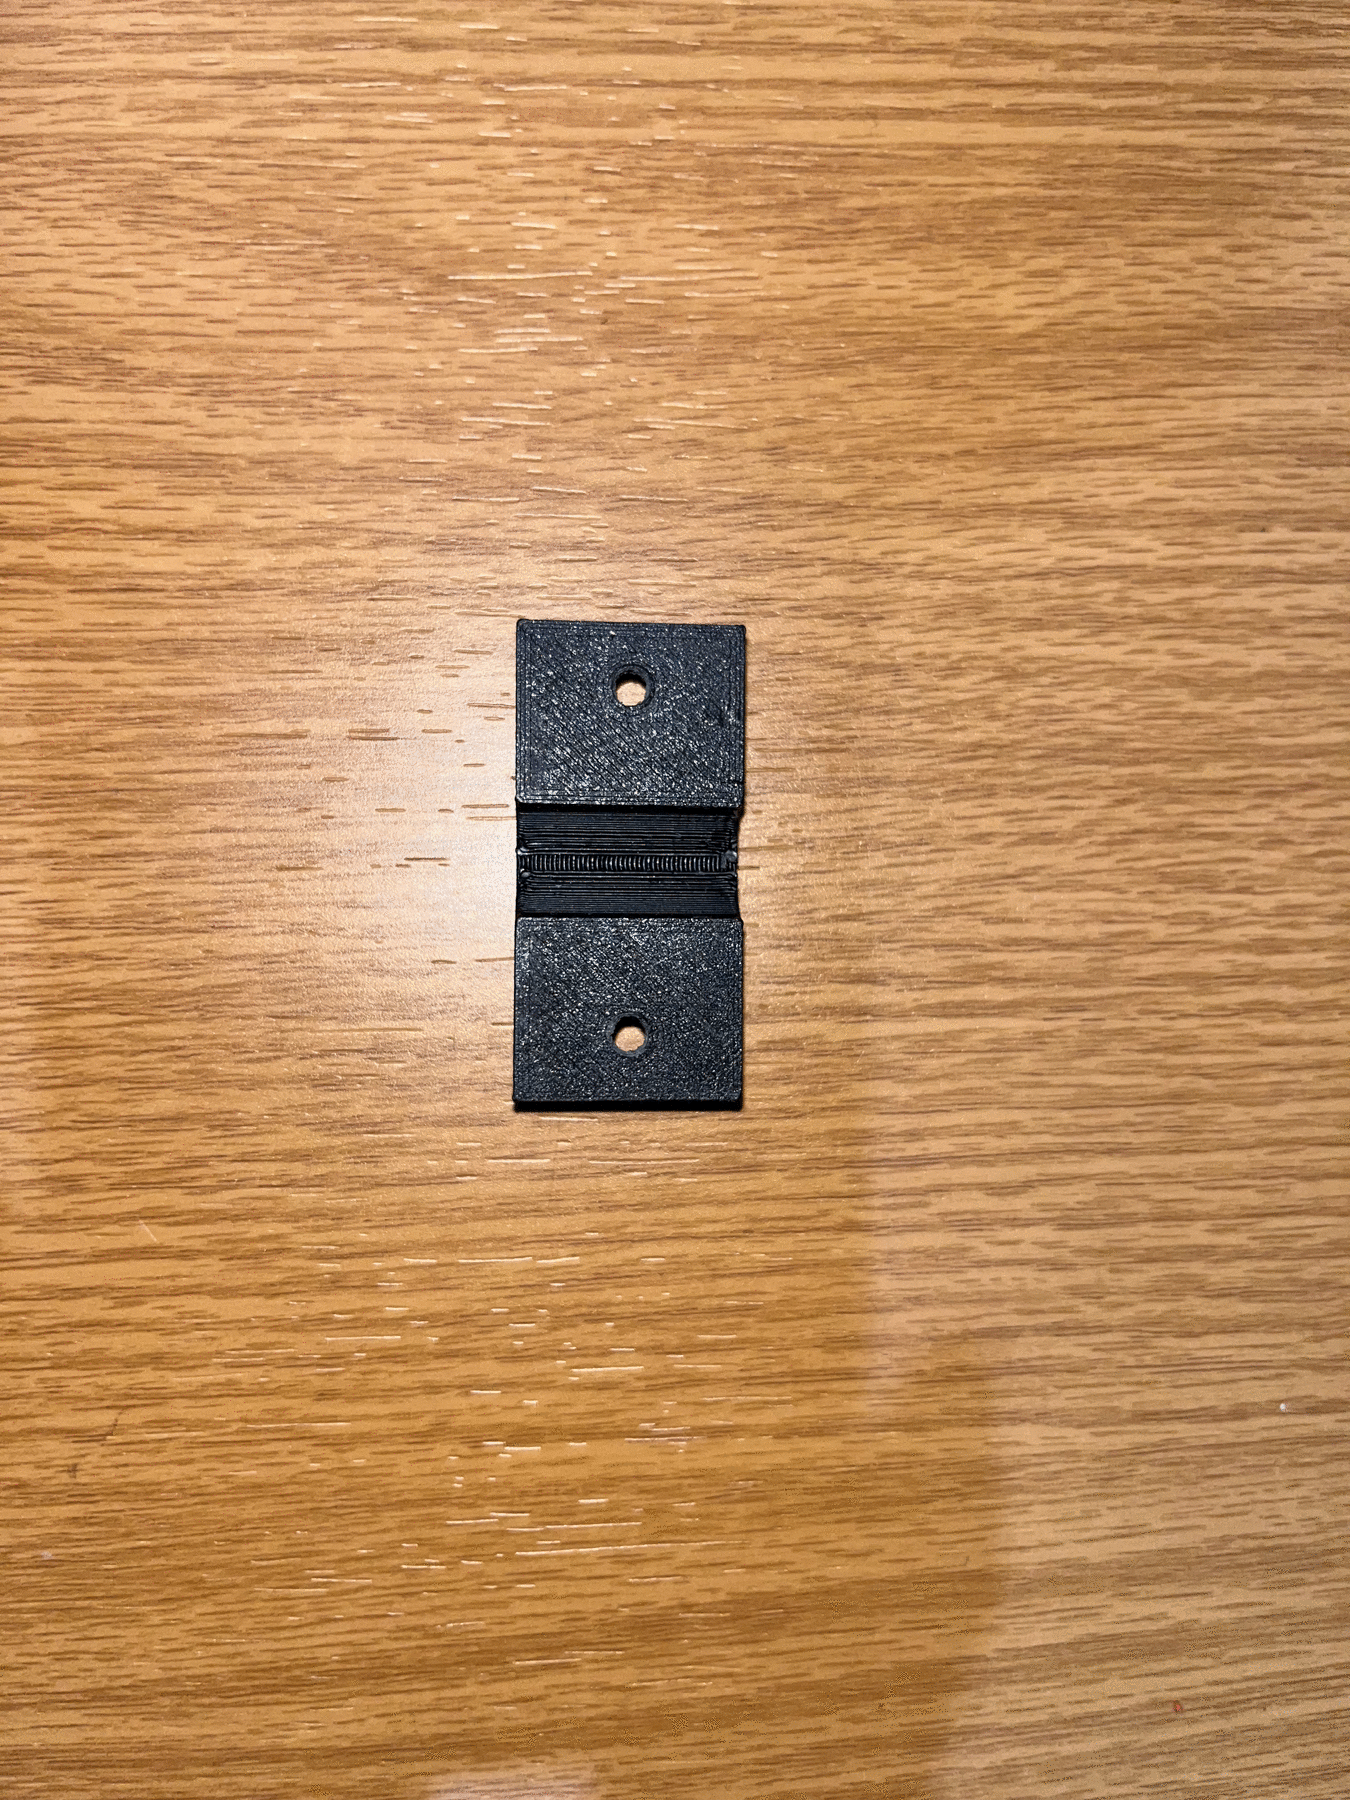
\includegraphics[width=0.7\linewidth]{bab3/top_plate_real2}
				\caption{Hasil Realisasi Plat Pengikat Kompartemen Tampak Perspektif 2}
				\label{fig:top-plate-real-2}
			\end{subfigure}
		\end{figure}
		\item Casing baterai (Desain Awal)\\
		\begin{figure}[H]
			\centering
			\begin{subfigure}[b]{0.45\textwidth}
				\centering
				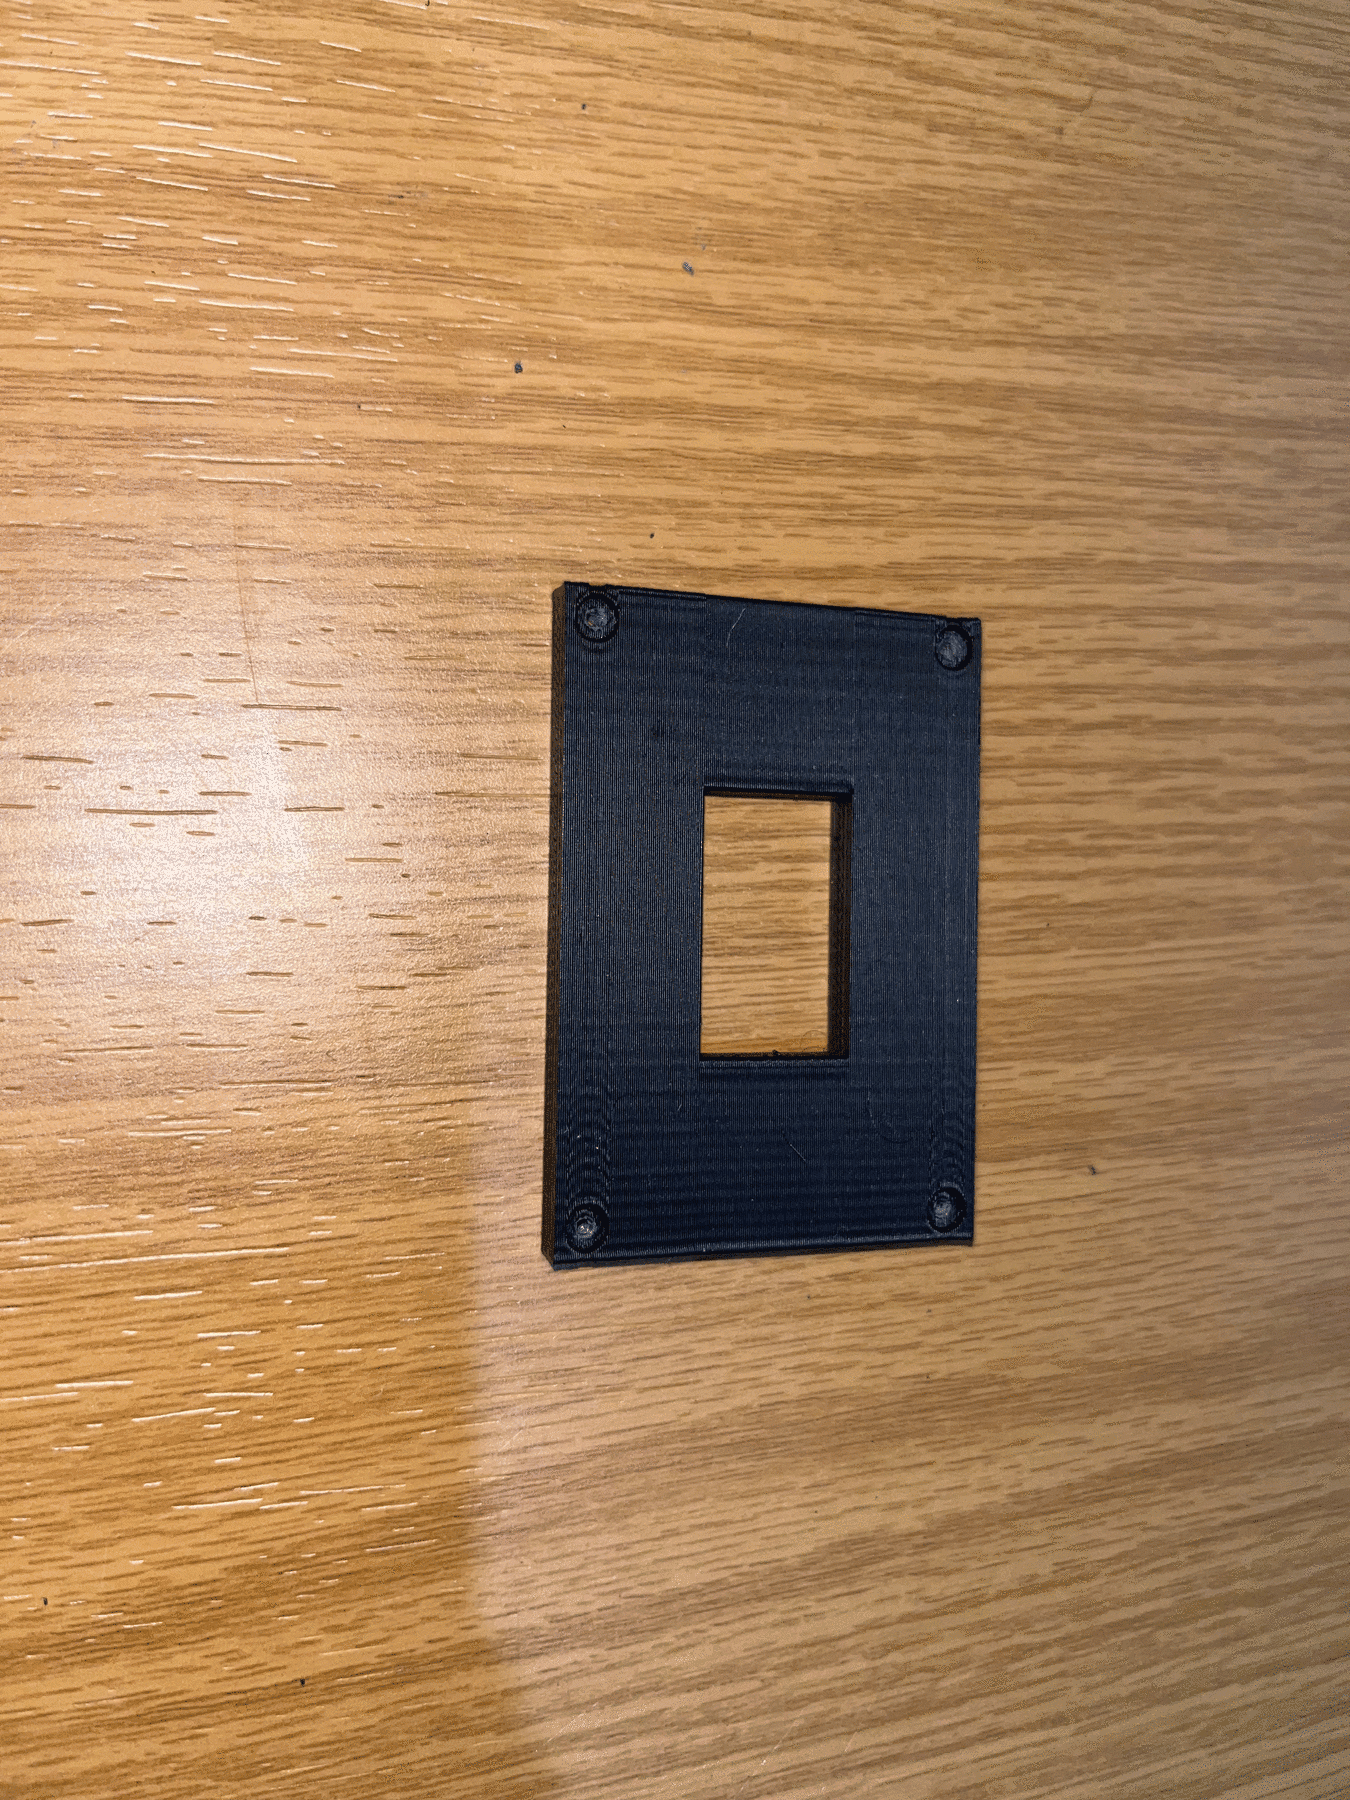
\includegraphics[width=0.7\linewidth]{bab3/casing_baterai_real1}
				\caption{Hasil Realisasi Casing baterai Tampak Perspektif 1 (Desain Awal)}
				\label{fig:retainer-baterai-real-1}
			\end{subfigure}
			\hfill
			\begin{subfigure}[b]{0.45\textwidth}
				\centering
				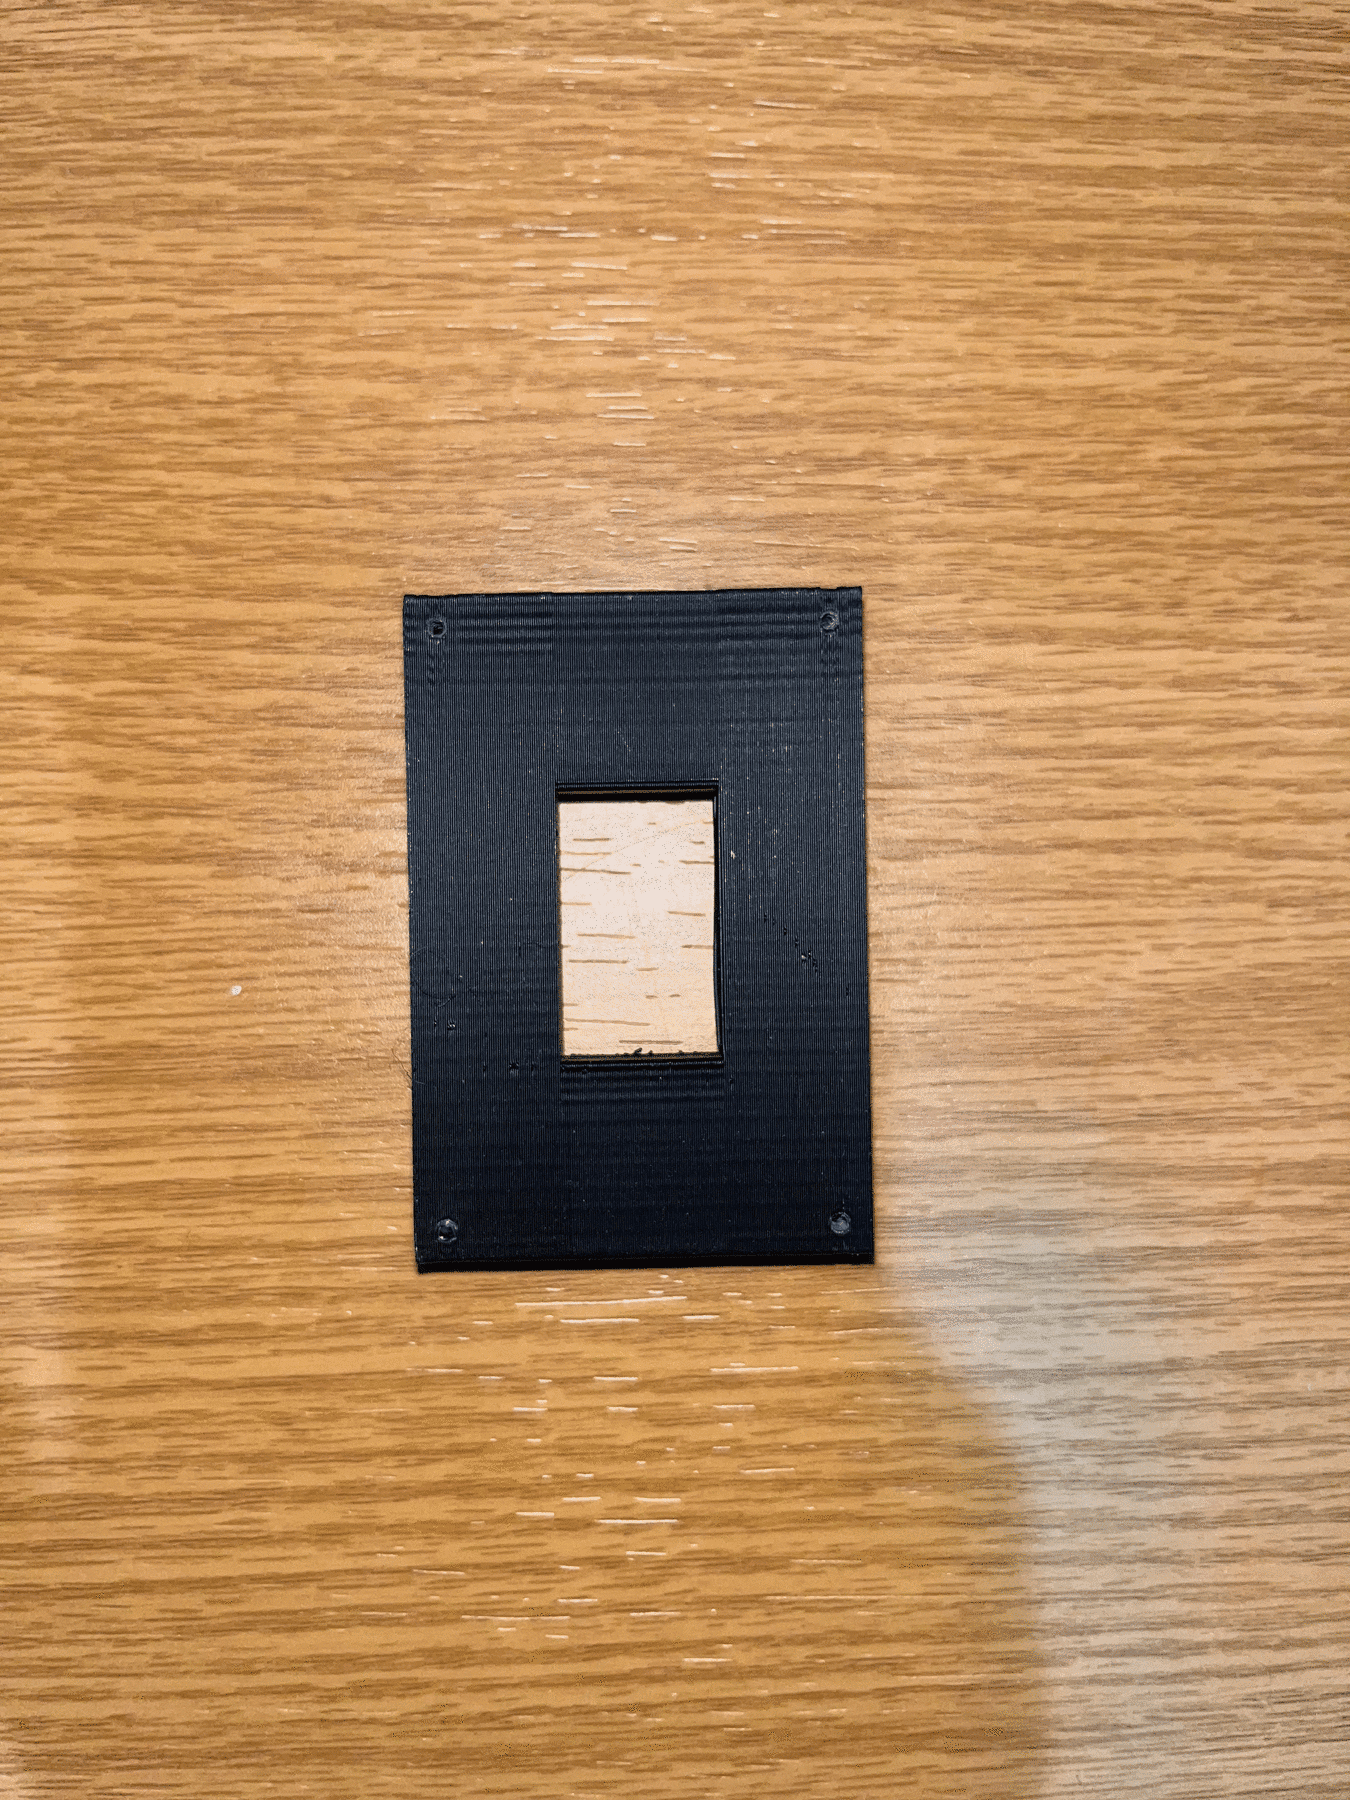
\includegraphics[width=0.7\linewidth]{bab3/casing_baterai_real2}
				\caption{Hasil Realisasi Casing baterai Tampak Perspektif 2 (Desain Awal)}
				\label{fig:retainer-baterai-real-2}
			\end{subfigure}
		\end{figure}
		\item Casing Raspberry Pi (Desain Awal)\\
		\begin{figure}[H]
			\centering
			\begin{subfigure}[b]{0.45\textwidth}
				\centering
				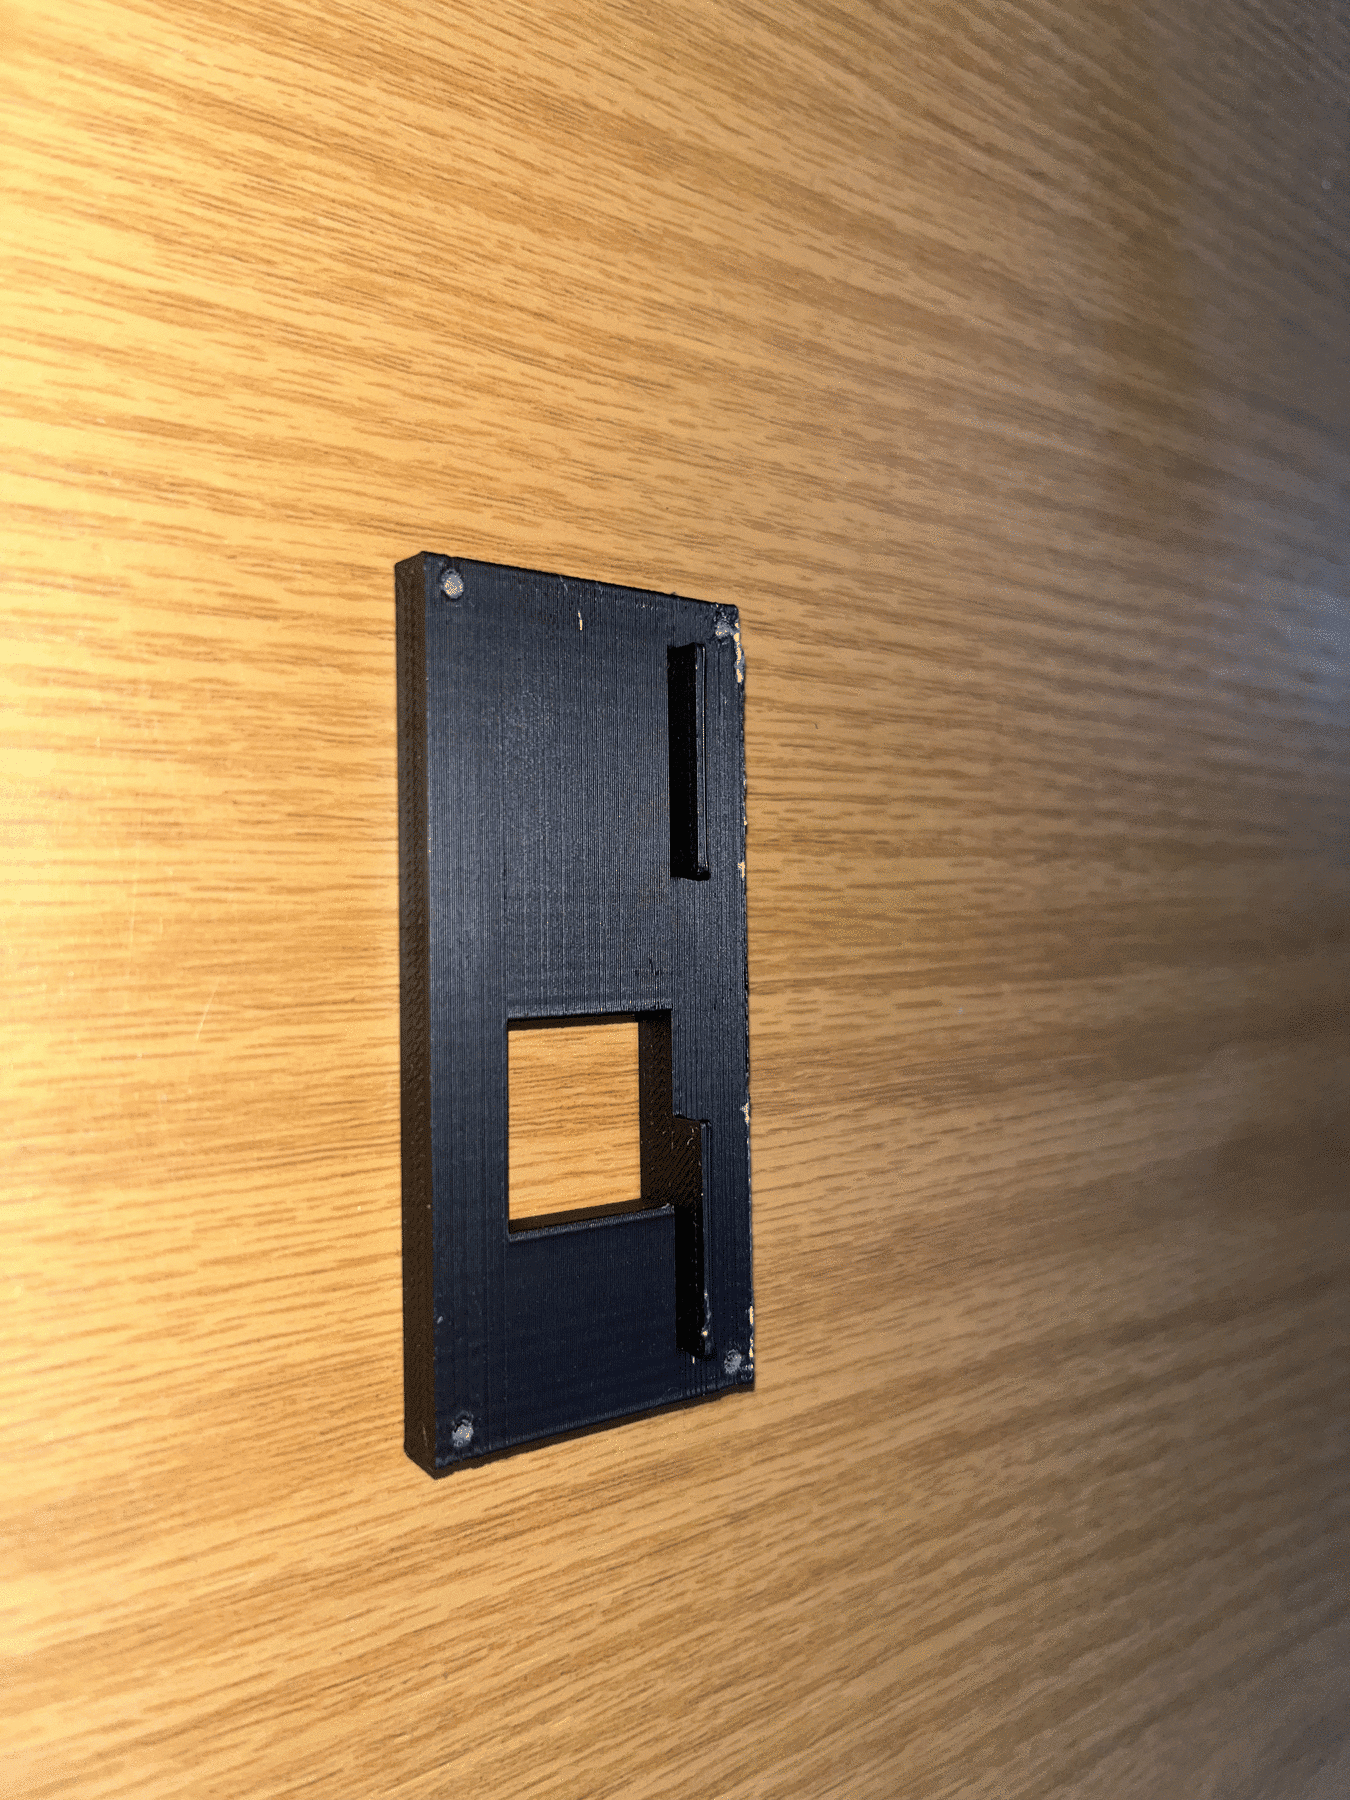
\includegraphics[width=0.7\linewidth]{bab3/casing_raspberry_pi_real1}
				\caption{Hasil Realisasi Casing Raspberry Pi Tampak Perspektif 1 (Desain Awal)}
				\label{fig:rpi5-cover-real-1}
			\end{subfigure}
			\hfill
			\begin{subfigure}[b]{0.45\textwidth}
				\centering
				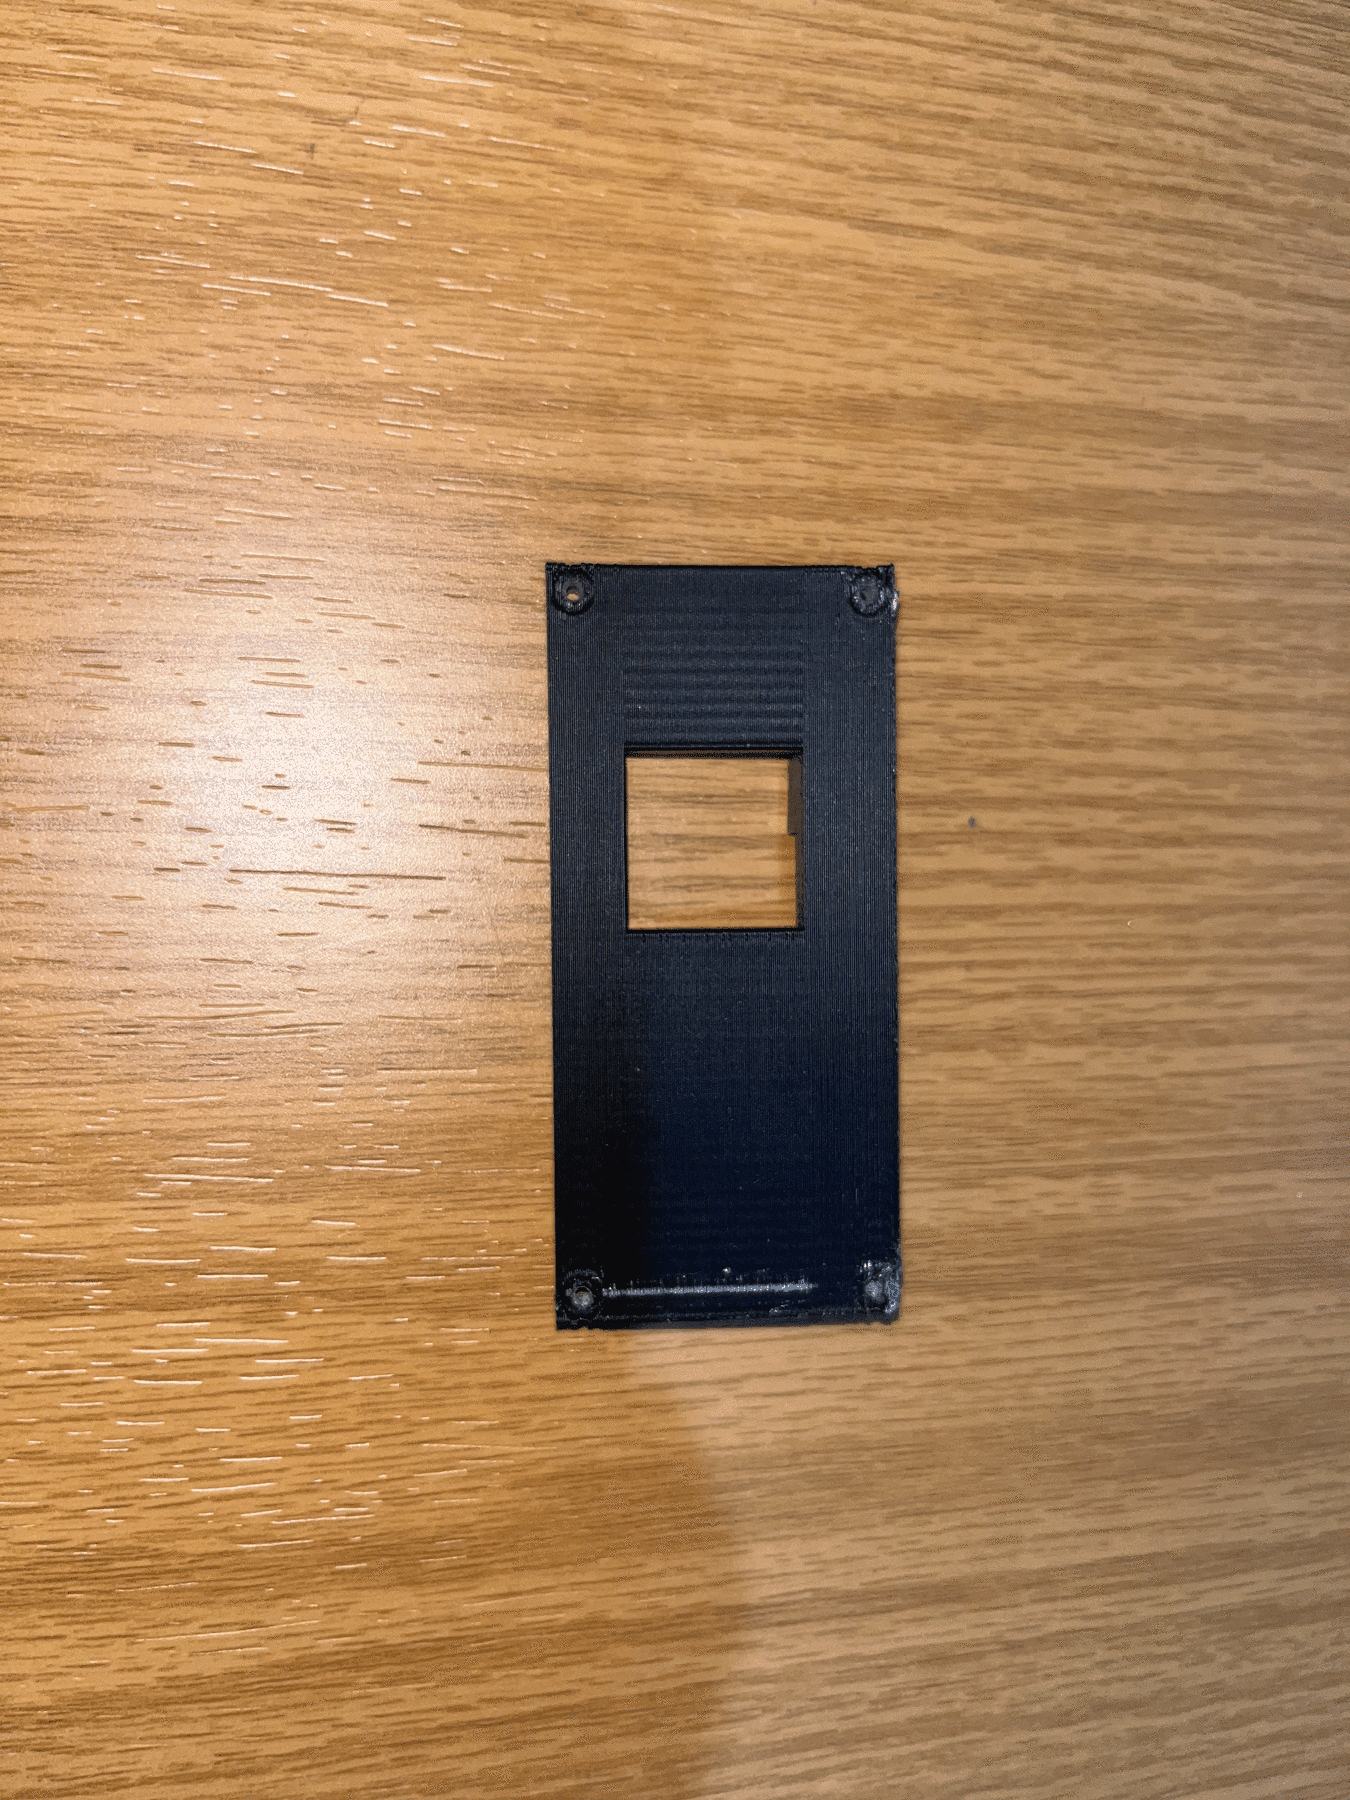
\includegraphics[width=0.7\linewidth]{bab3/casing_raspberry_pi_real2}
				\caption{Hasil Realisasi Casing Raspberry Pi Tampak Perspektif 2 (Desain Awal)}
				\label{fig:rpi5-cover-real-2}
			\end{subfigure}
		\end{figure}
		\item Casing power supply (Desain Awal)\\
		\begin{figure}[H]
			\centering
			\begin{subfigure}[b]{0.45\textwidth}
				\centering
				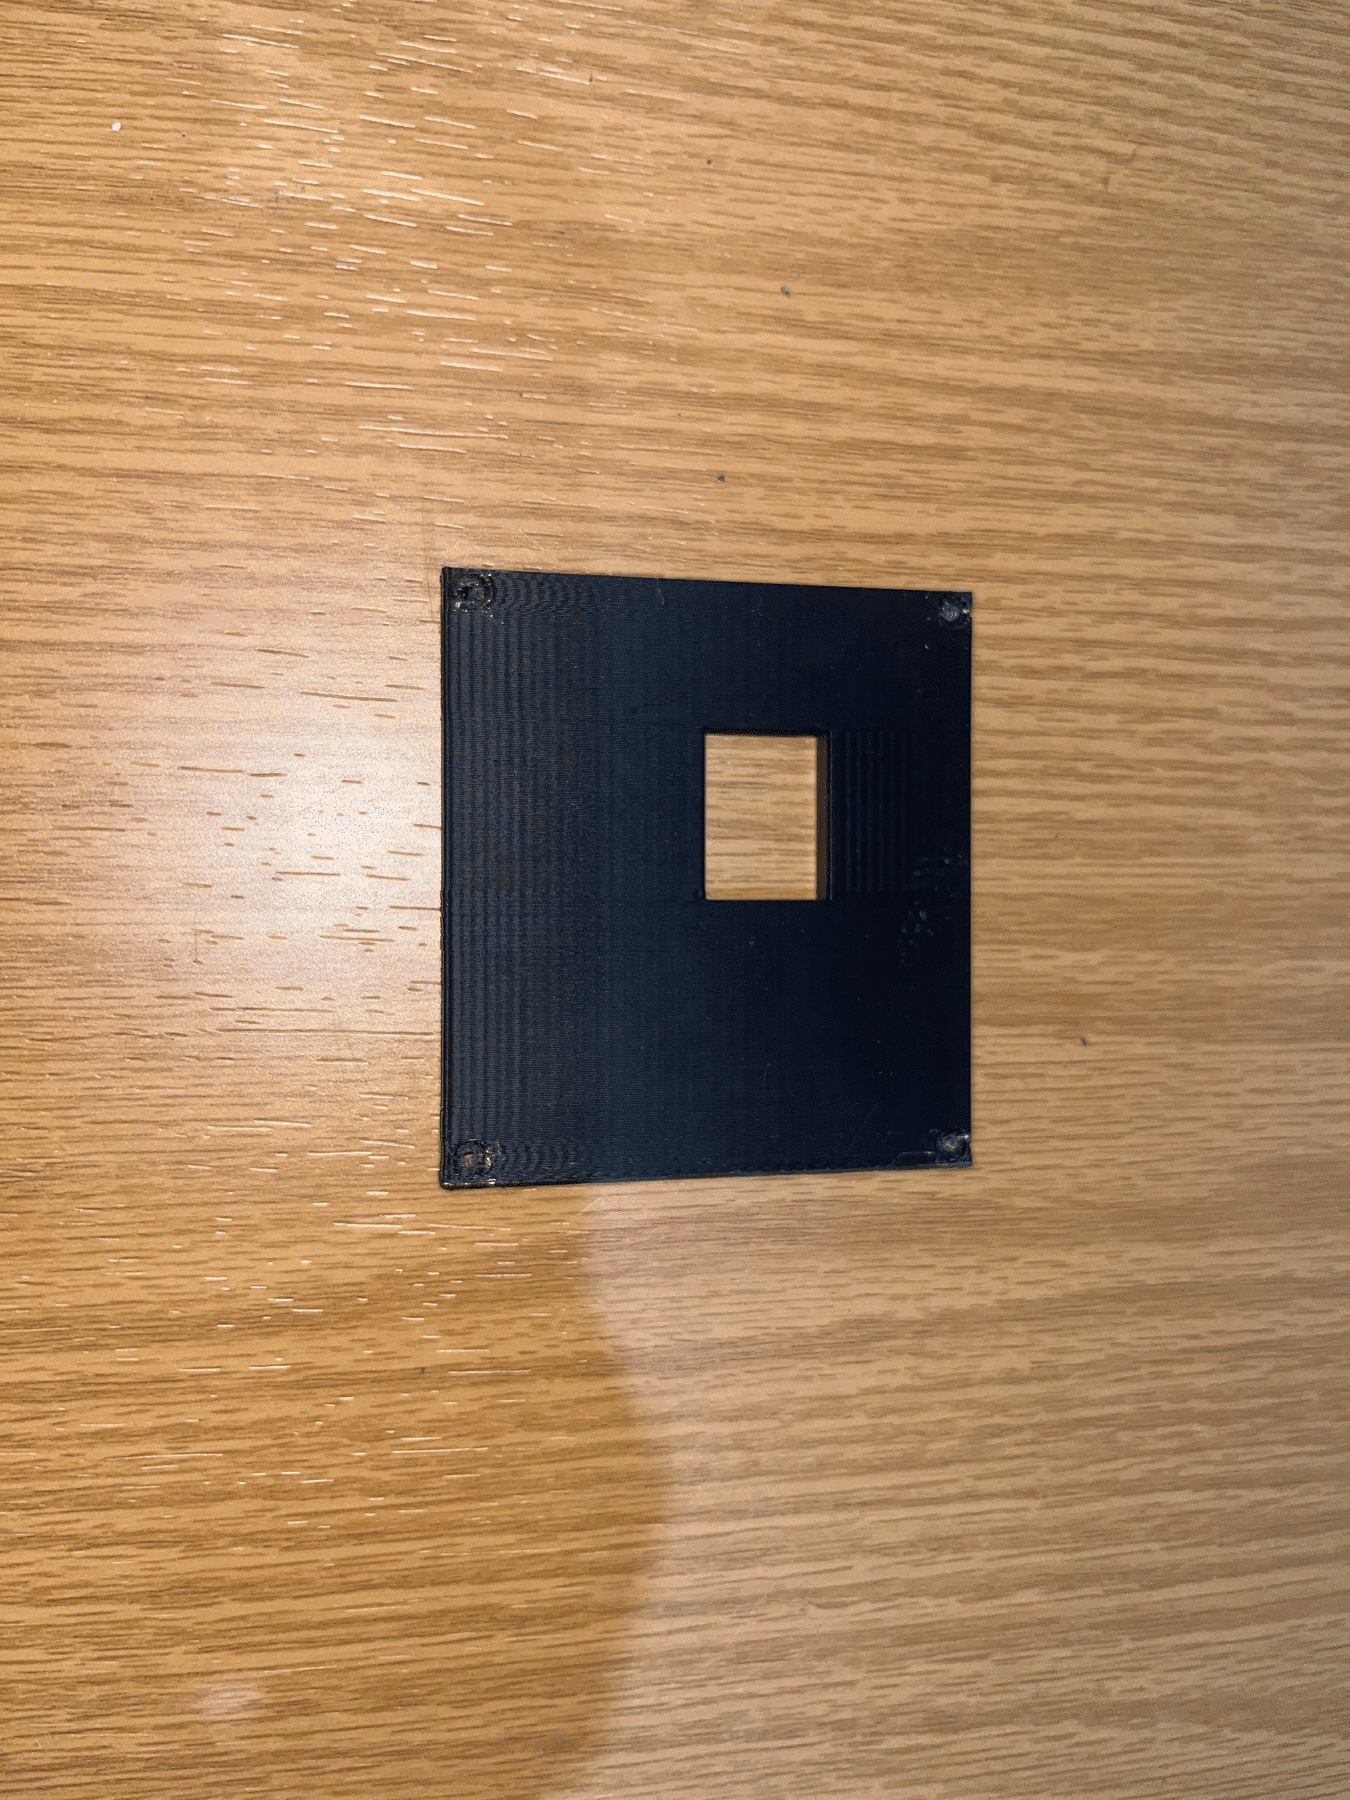
\includegraphics[width=0.7\linewidth]{bab3/casing_power_supply_real1}
				\caption{Hasil Realisasi Casing power supply Tampak Perspektif 1 (Desain Awal)}
				\label{fig:ubec-cover-real-1}
			\end{subfigure}
			\hfill
			\begin{subfigure}[b]{0.45\textwidth}
				\centering
				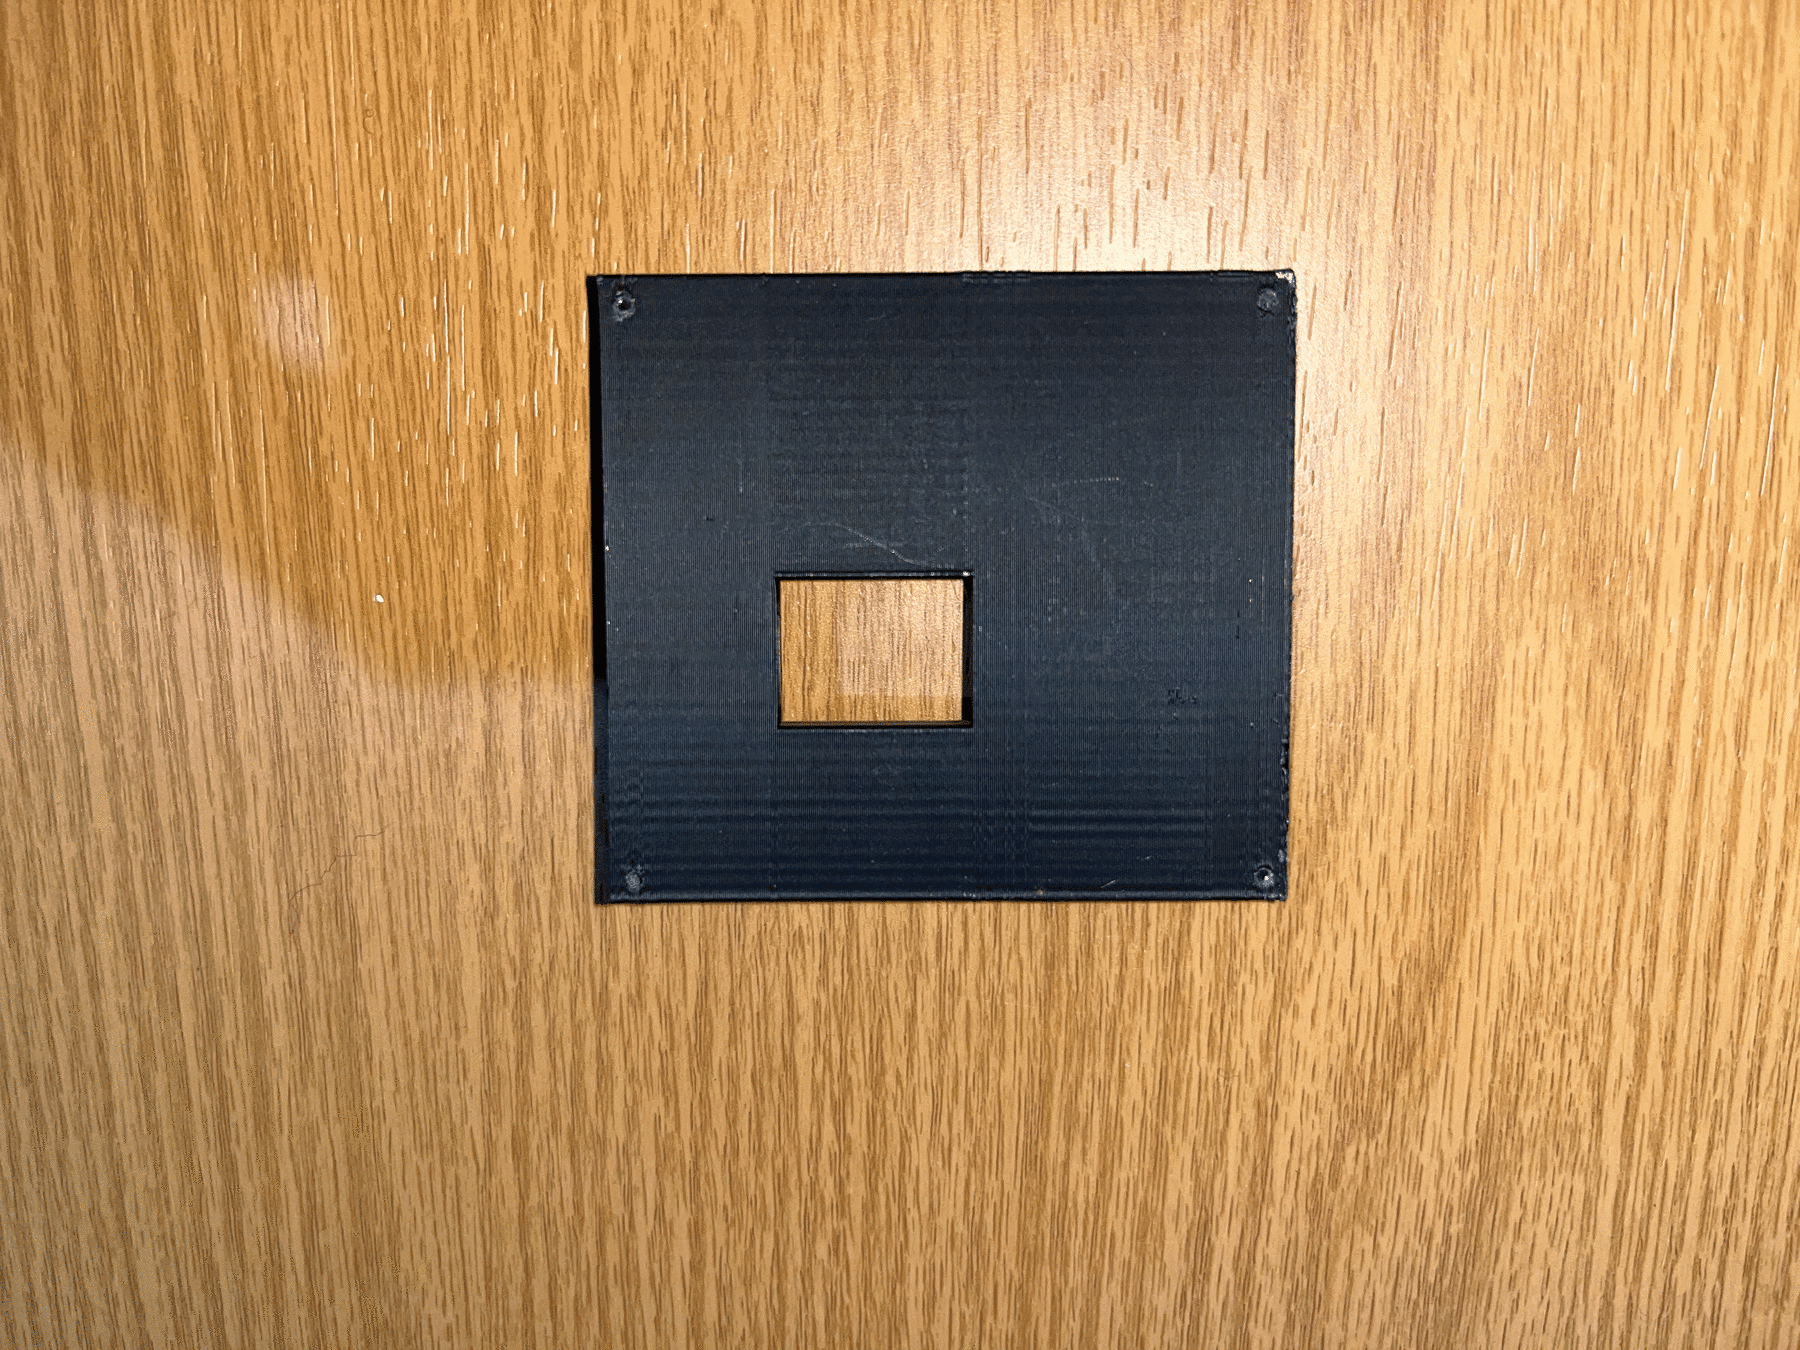
\includegraphics[width=0.7\linewidth]{bab3/casing_power_supply_real2}
				\caption{Hasil Realisasi Casing power supply Tampak Perspektif 2 (Desain Awal)}
				\label{fig:ubec-cover-real-2}
			\end{subfigure}
		\end{figure}
		\item Casing kamera (Desain Awal)\\
		\begin{figure}[H]
			\centering
			\begin{subfigure}[b]{0.3\textwidth}
				\centering
				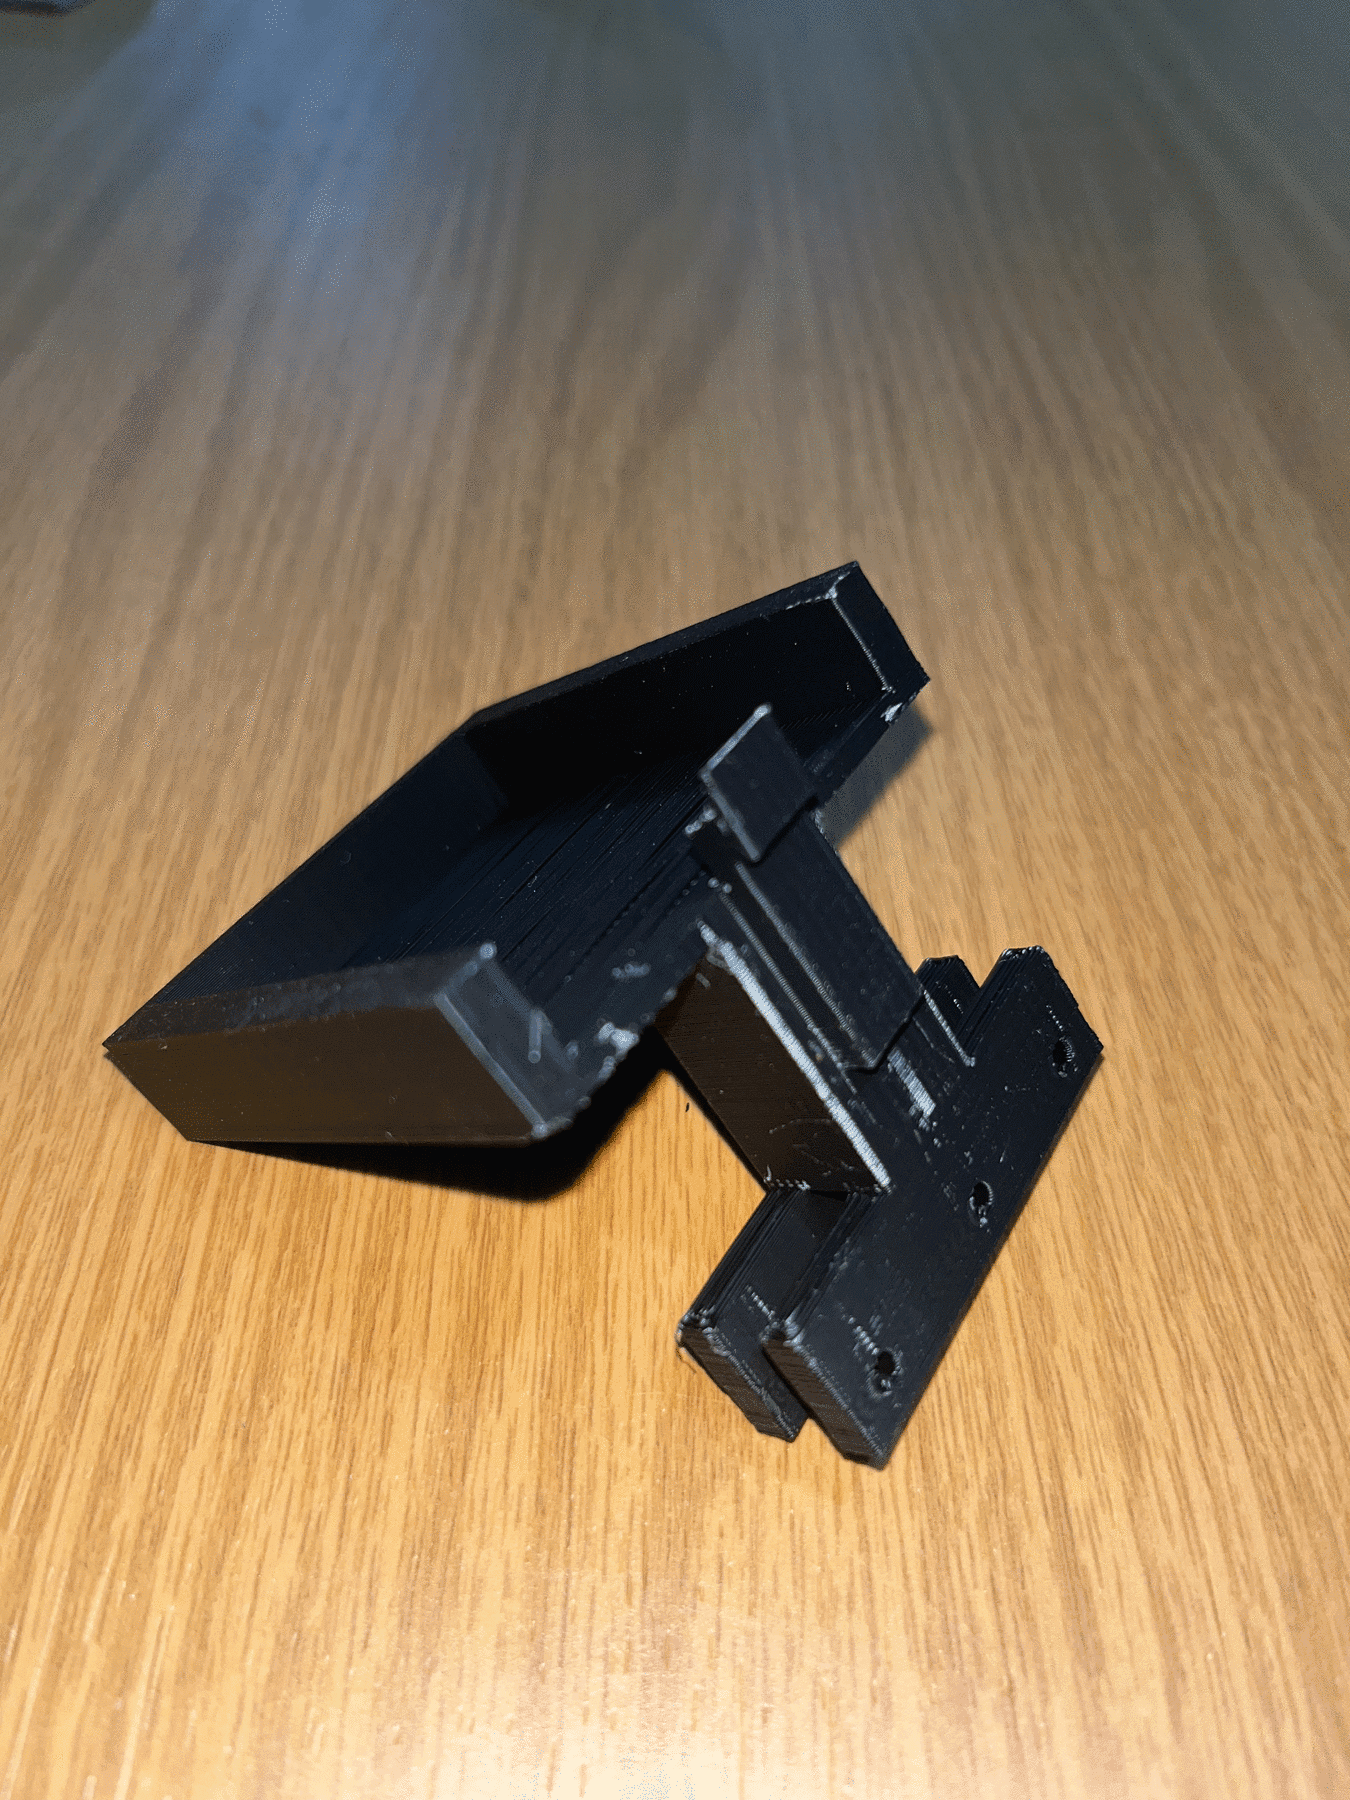
\includegraphics[width=0.7\linewidth]{bab3/casing_kamera_real1}
				\caption{Hasil Realisasi Casing kamera Tampak Perspektif 1 (Desain Awal)}
				\label{fig:webcam-back-real-1}
			\end{subfigure}
			\hfill
			\begin{subfigure}[b]{0.3\textwidth}
				\centering
				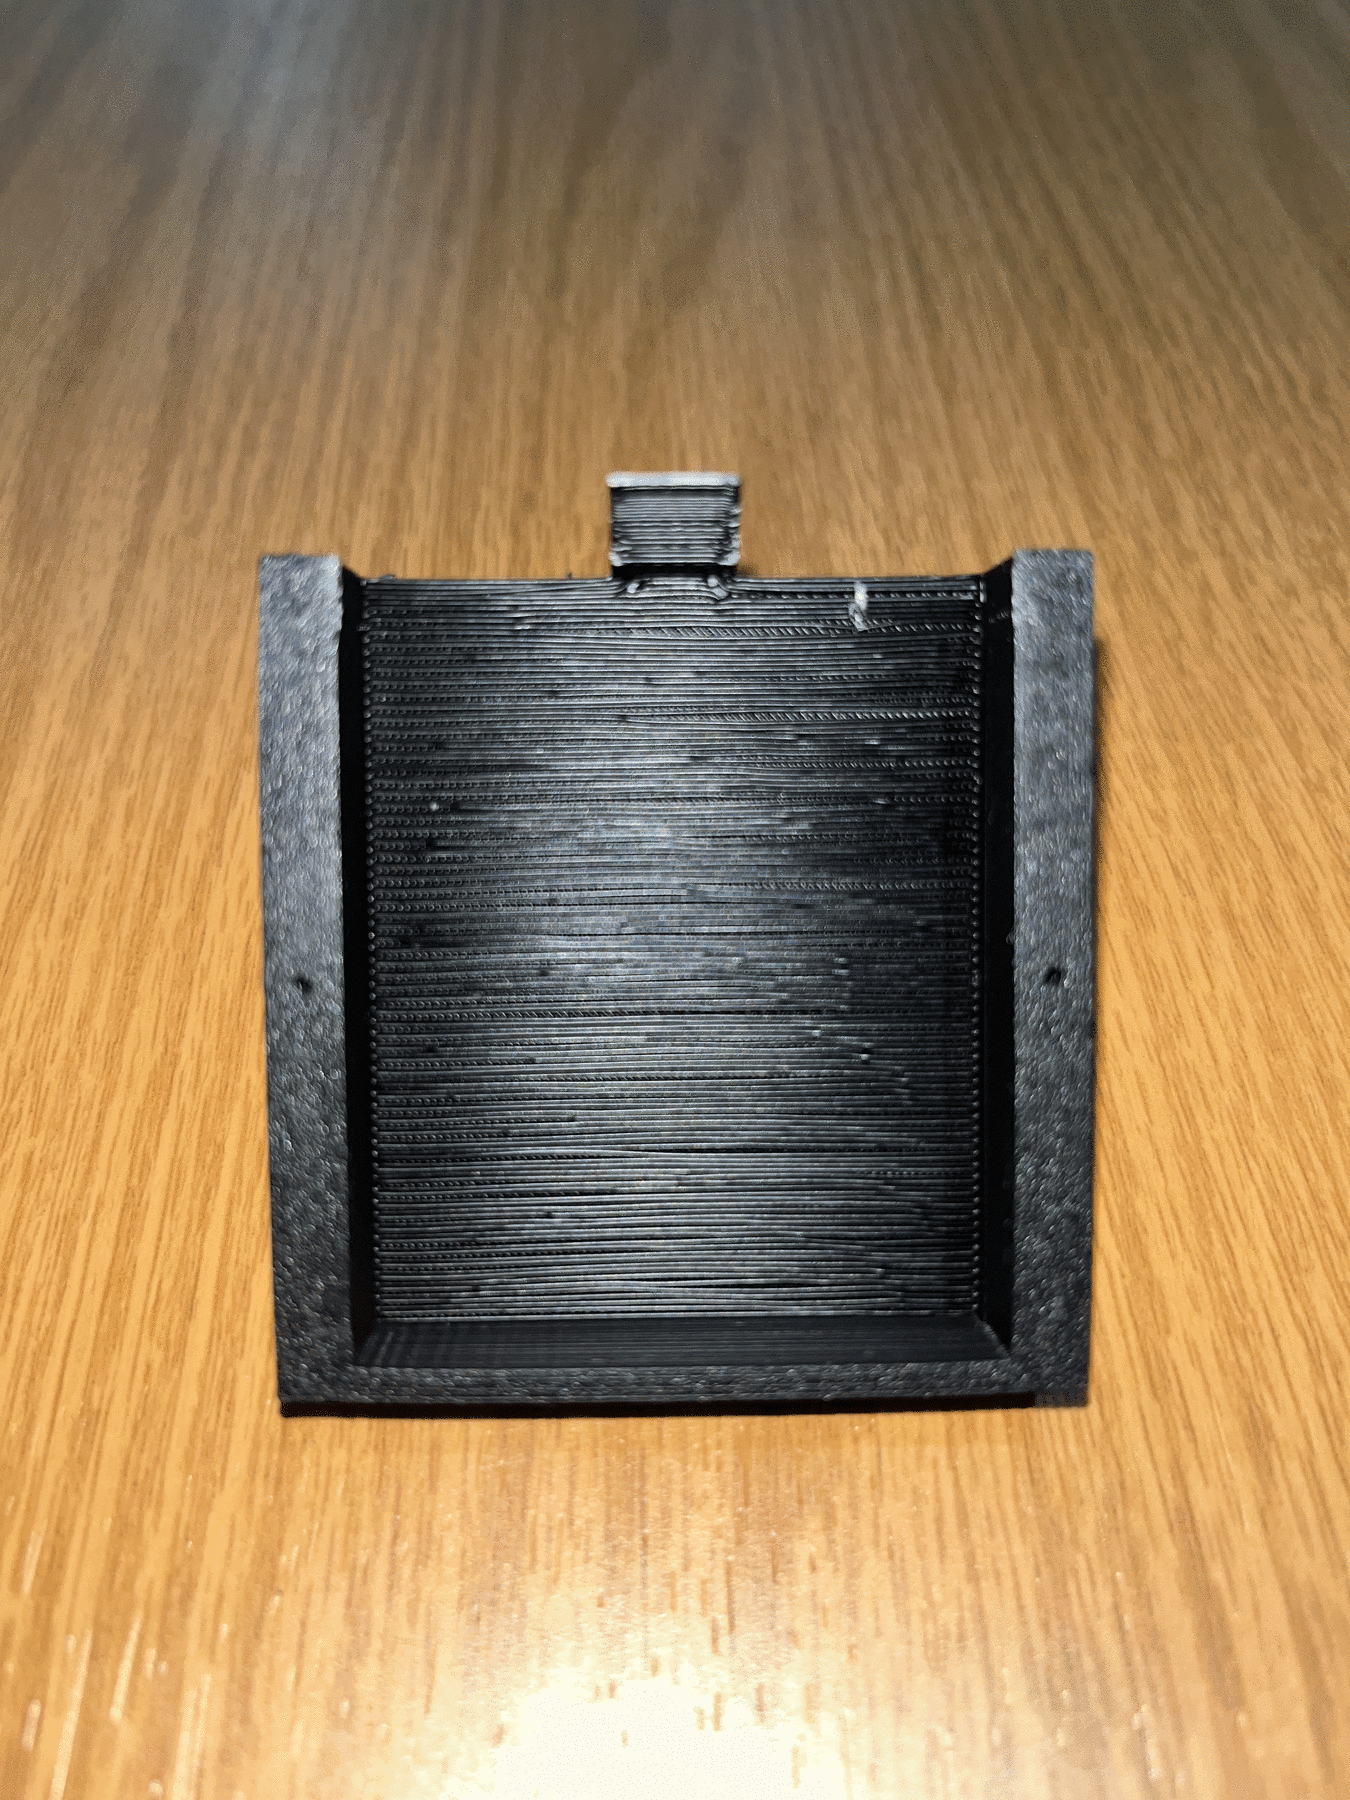
\includegraphics[width=0.7\linewidth]{bab3/casing_kamera_real2}
				\caption{Hasil Realisasi Casing kamera Tampak Perspektif 2 (Desain Awal)}
				\label{fig:webcam-back-real-2}
			\end{subfigure}
			\hfill
			\begin{subfigure}[b]{0.3\textwidth}
				\centering
				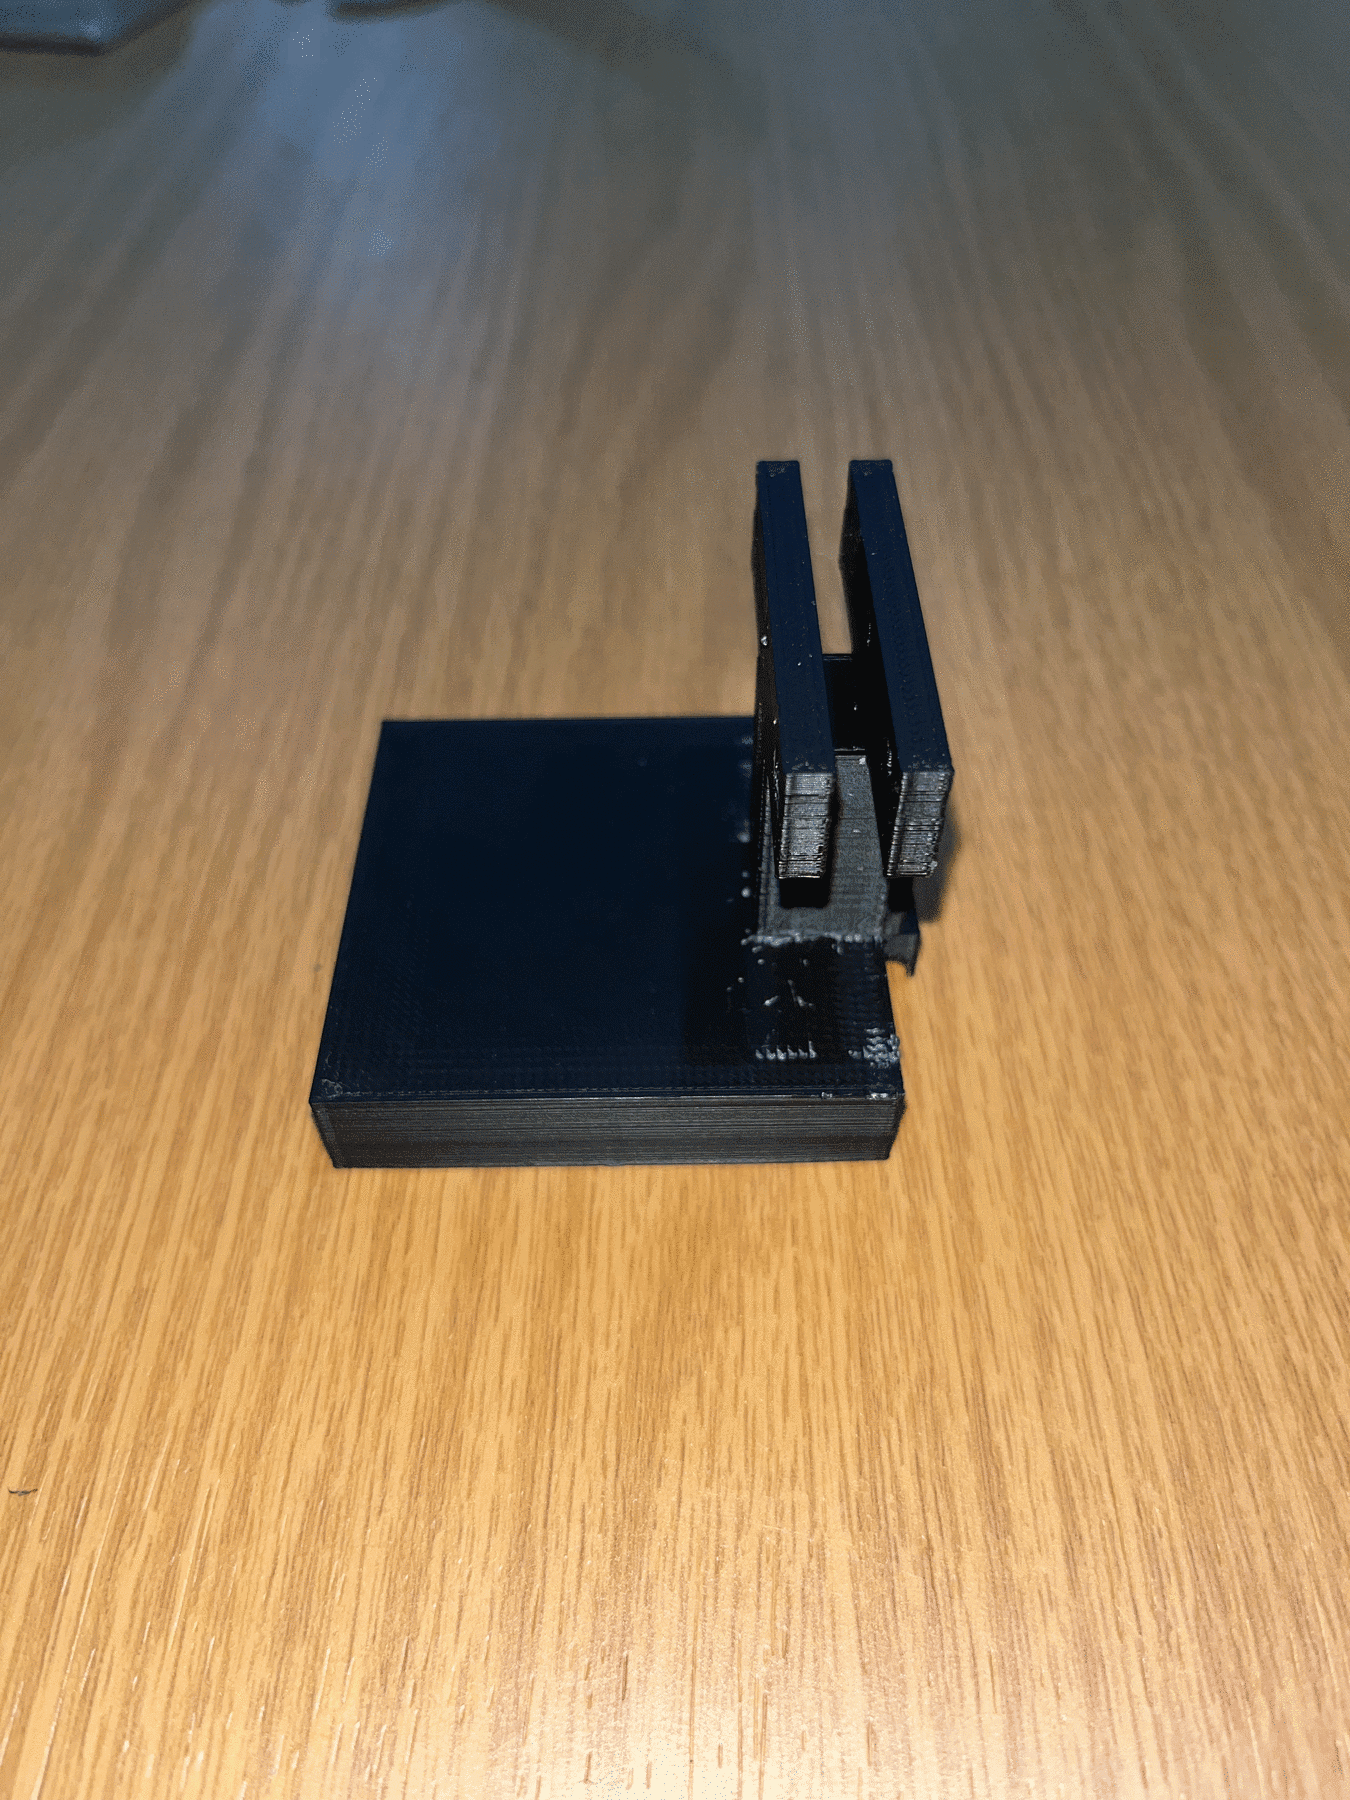
\includegraphics[width=0.7\linewidth]{bab3/casing_kamera_real3}
				\caption{Hasil Realisasi Casing kamera Tampak Perspektif 3 (Desain Awal)}
				\label{fig:webcam-back-real-3}
			\end{subfigure}
		\end{figure}
		\item Tutup kamera (Desain Awal)\\
		\begin{figure}[H]
			\centering
			\begin{subfigure}[b]{0.45\textwidth}
				\centering
				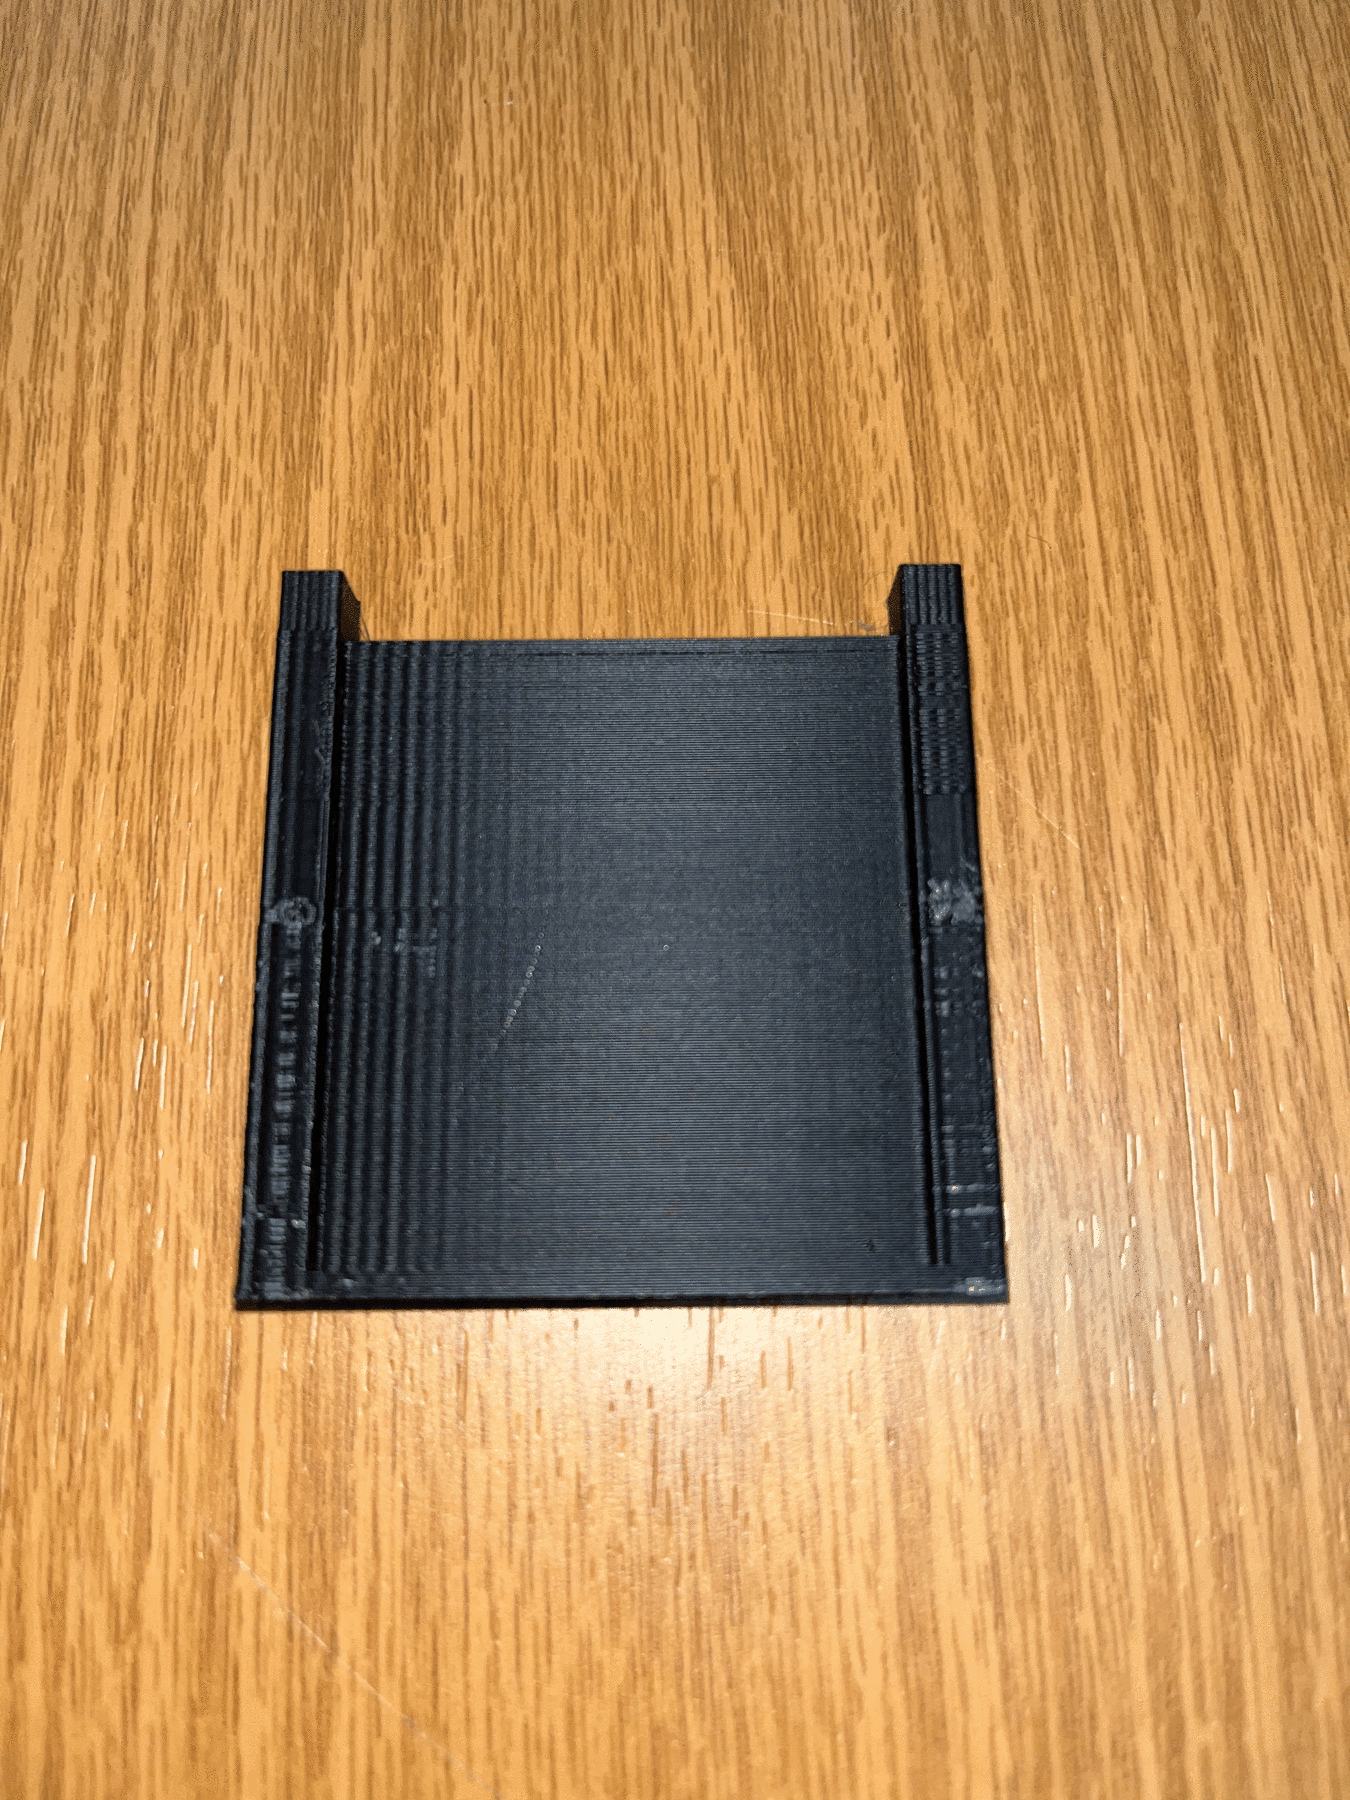
\includegraphics[width=0.7\linewidth]{bab3/tutup_kamera_real1}
				\caption{Hasil Realisasi Tutup kamera Tampak Perspektif 1 (Desain Awal)}
				\label{fig:webcam-front-real-1}
			\end{subfigure}
			\hfill
			\begin{subfigure}[b]{0.45\textwidth}
				\centering
				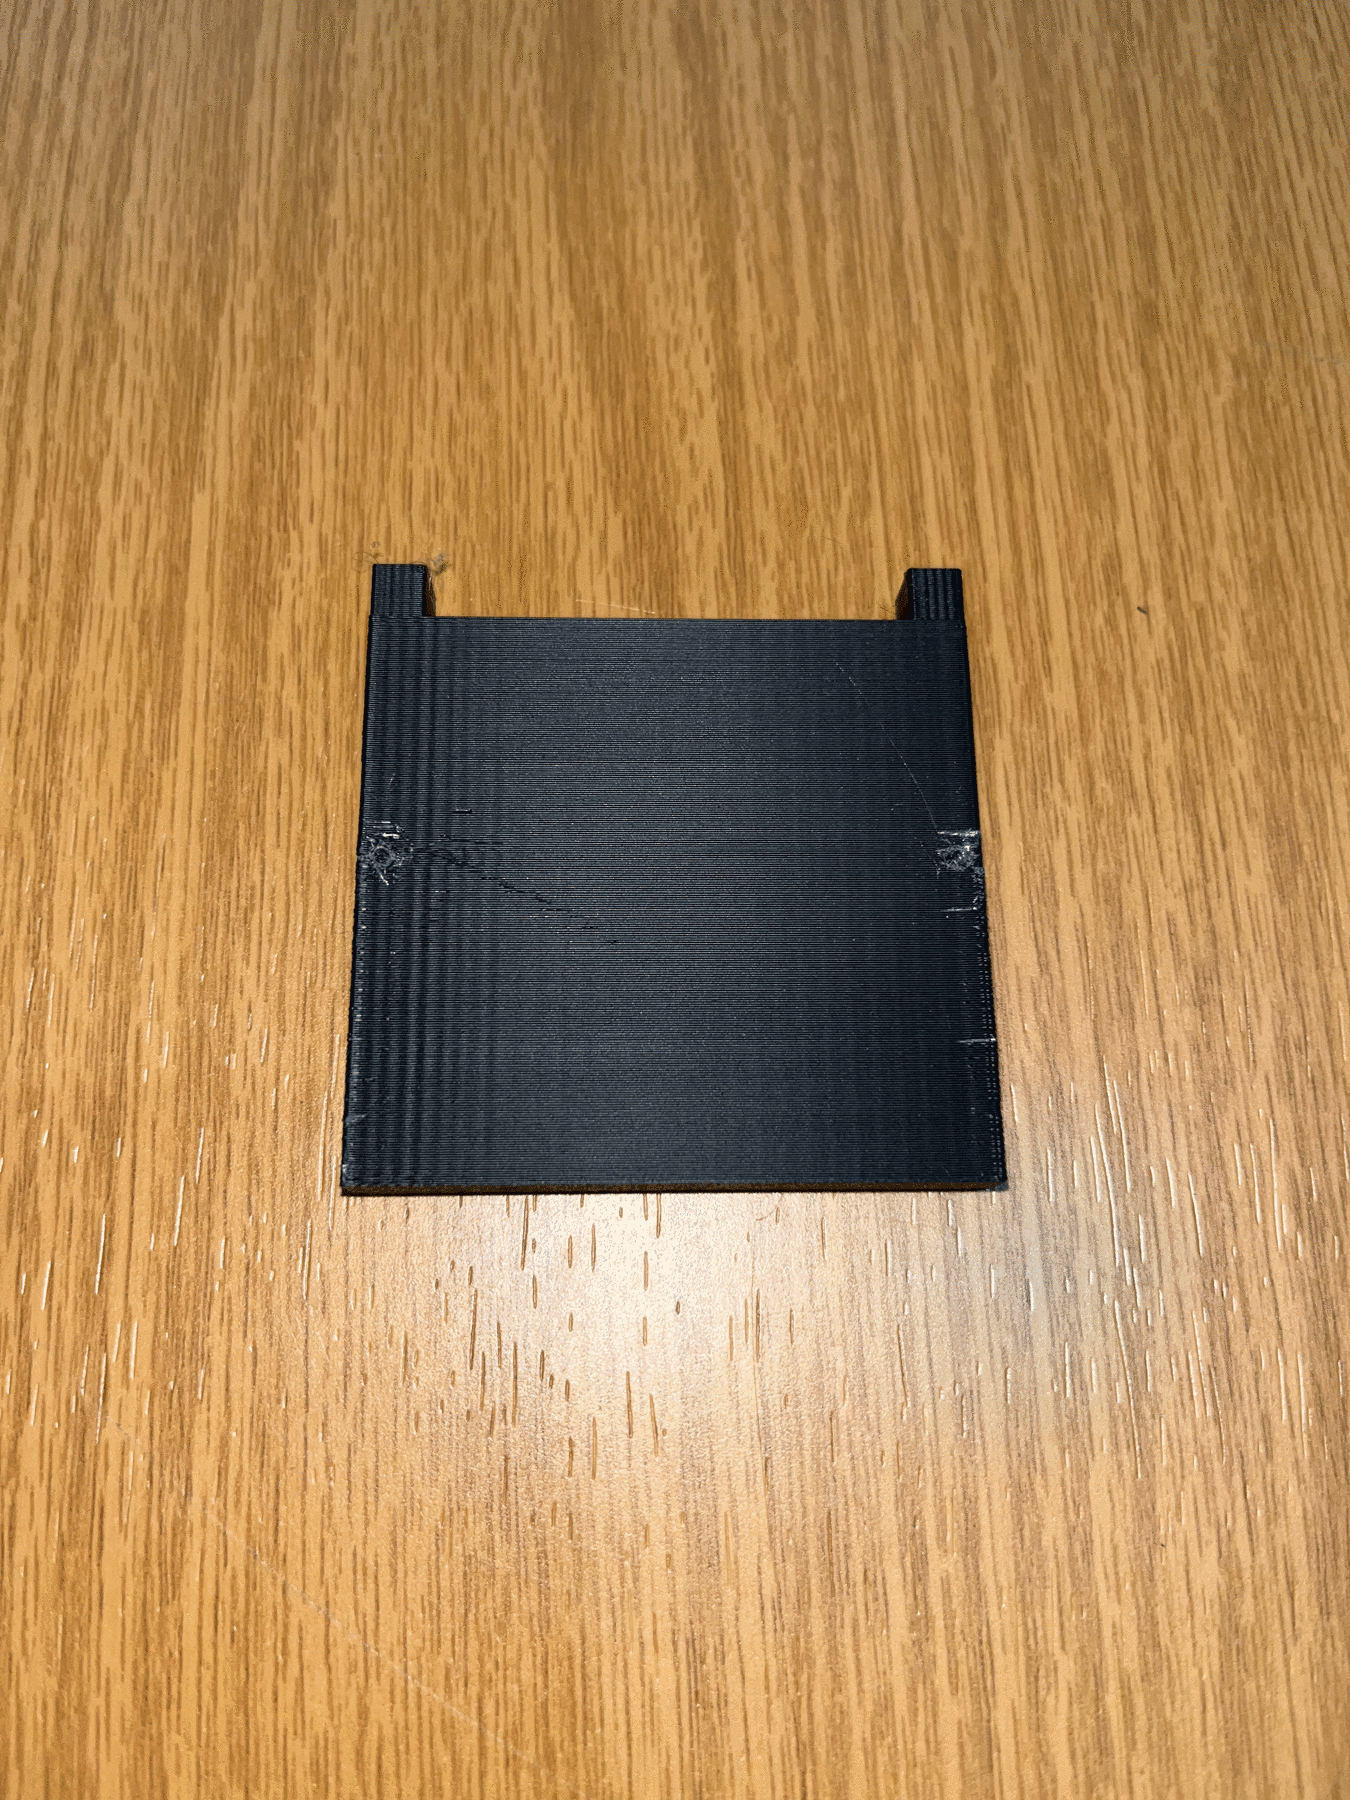
\includegraphics[width=0.7\linewidth]{bab3/tutup_kamera_real2}
				\caption{Hasil Realisasi Tutup kamera Tampak Perspektif 2 (Desain Awal)}
				\label{fig:webcam-front-real-2}
			\end{subfigure}
		\end{figure}
	\end{enumerate}
	
	\item Perakitan (Assembly) Komponen Mekanik 3D: Setelah seluruh komponen selesai dicetak, tahap selanjutnya adalah merakit komponen-komponen tersebut pada rangka bawah drone secara simetris. Penempatan yang terpusat ini bertujuan untuk meminimalisir pergeseran titik beban sehingga \textit{Center of Gravity} (CG) drone dapat terjaga. Berikut adalah hasil realisasi fisik perakitan keseluruhan komponen 3D pada sistem drone:
	
	\begin{figure}[H]
		\centering
		\begin{subfigure}[b]{0.3\textwidth}
			\centering
			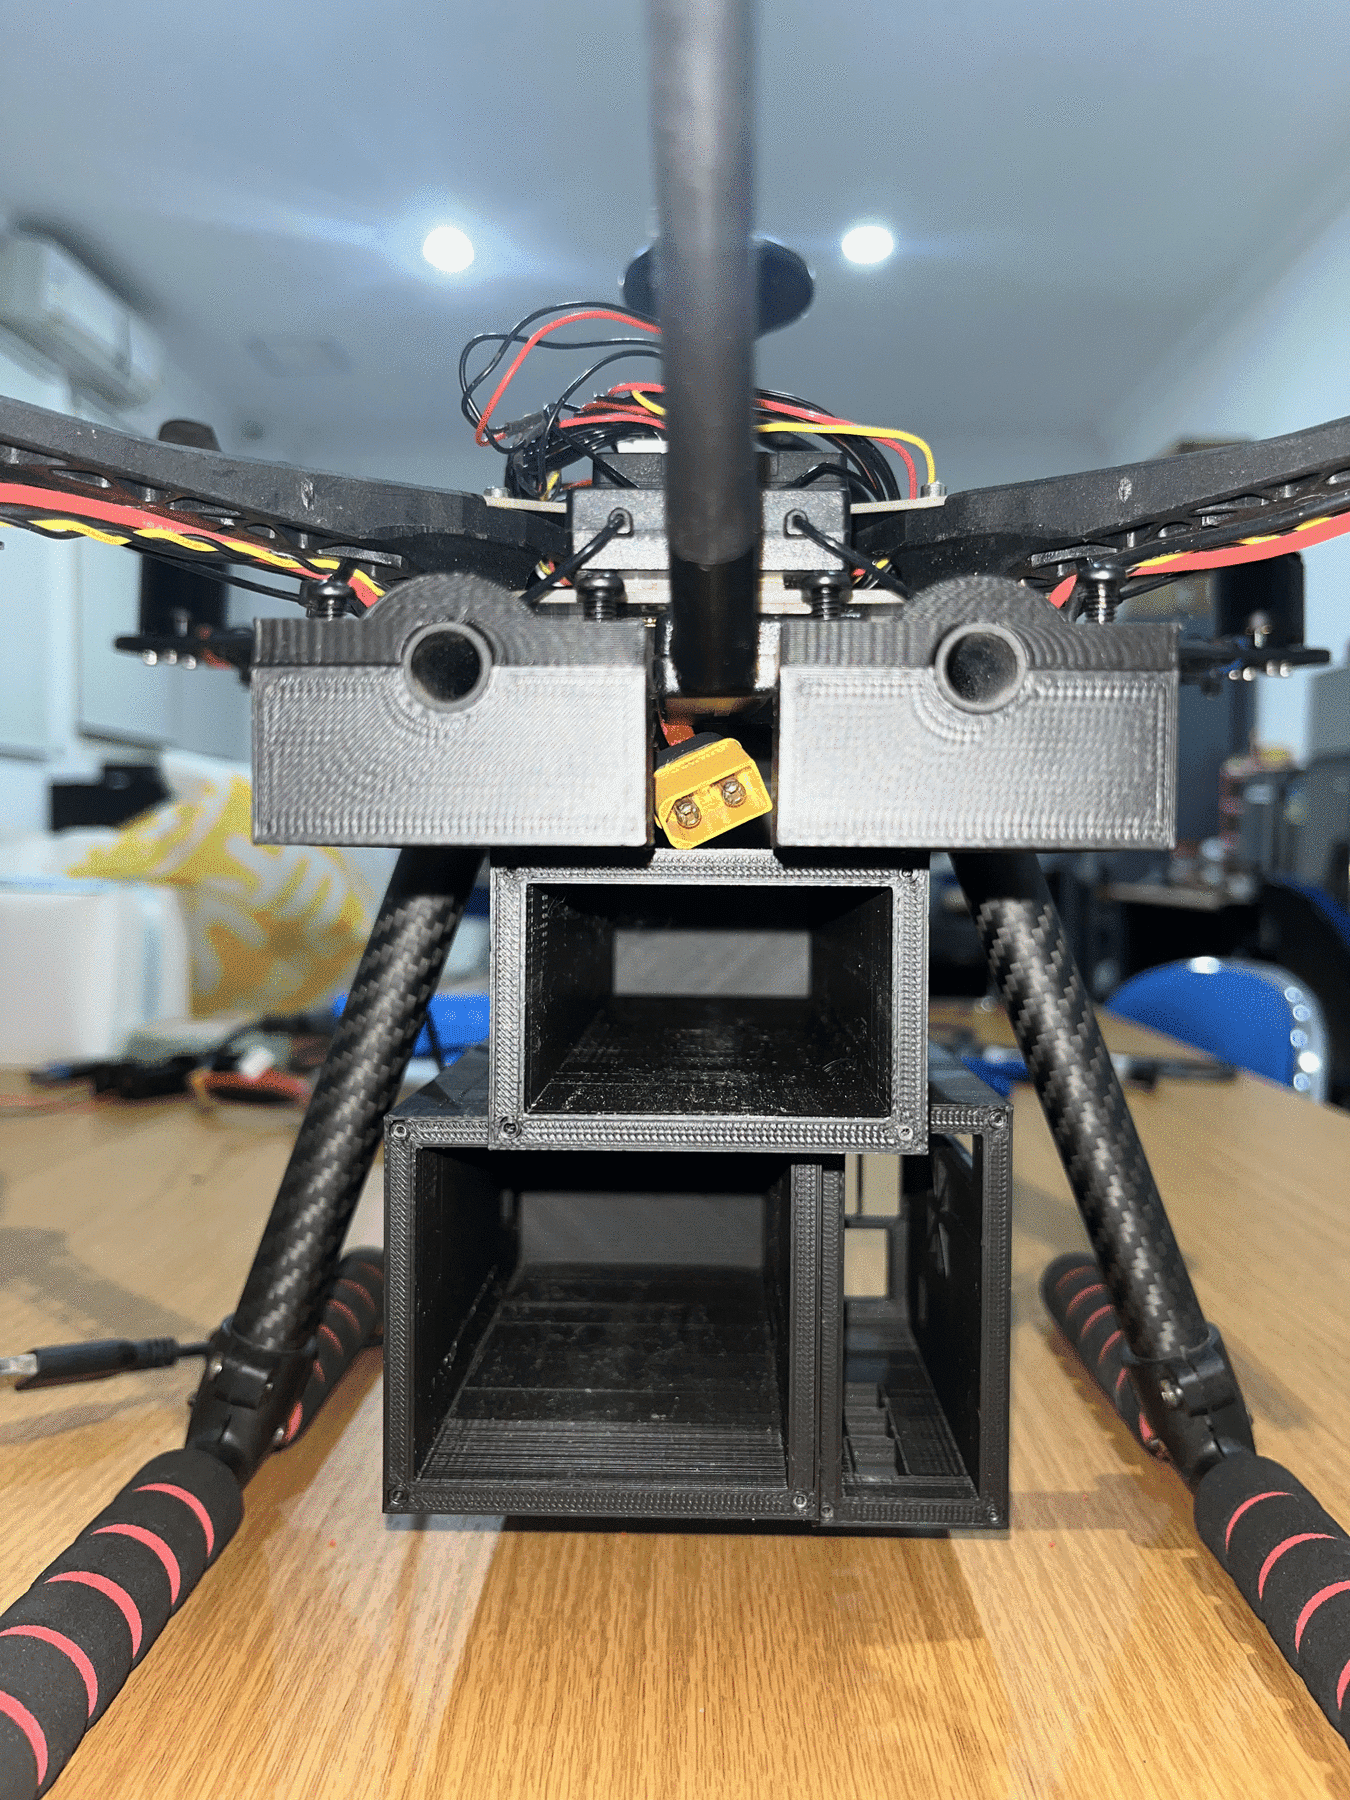
\includegraphics[width=0.7\linewidth]{bab3/full_assembly_real_1}
			\caption{Hasil Realisasi Perakitan Keseluruhan Sistem Tampak Perspektif 1}
			\label{fig:perakitan-keseluruhan-sistem-real-1}
		\end{subfigure}
		\hfill
		\begin{subfigure}[b]{0.3\textwidth}
			\centering
			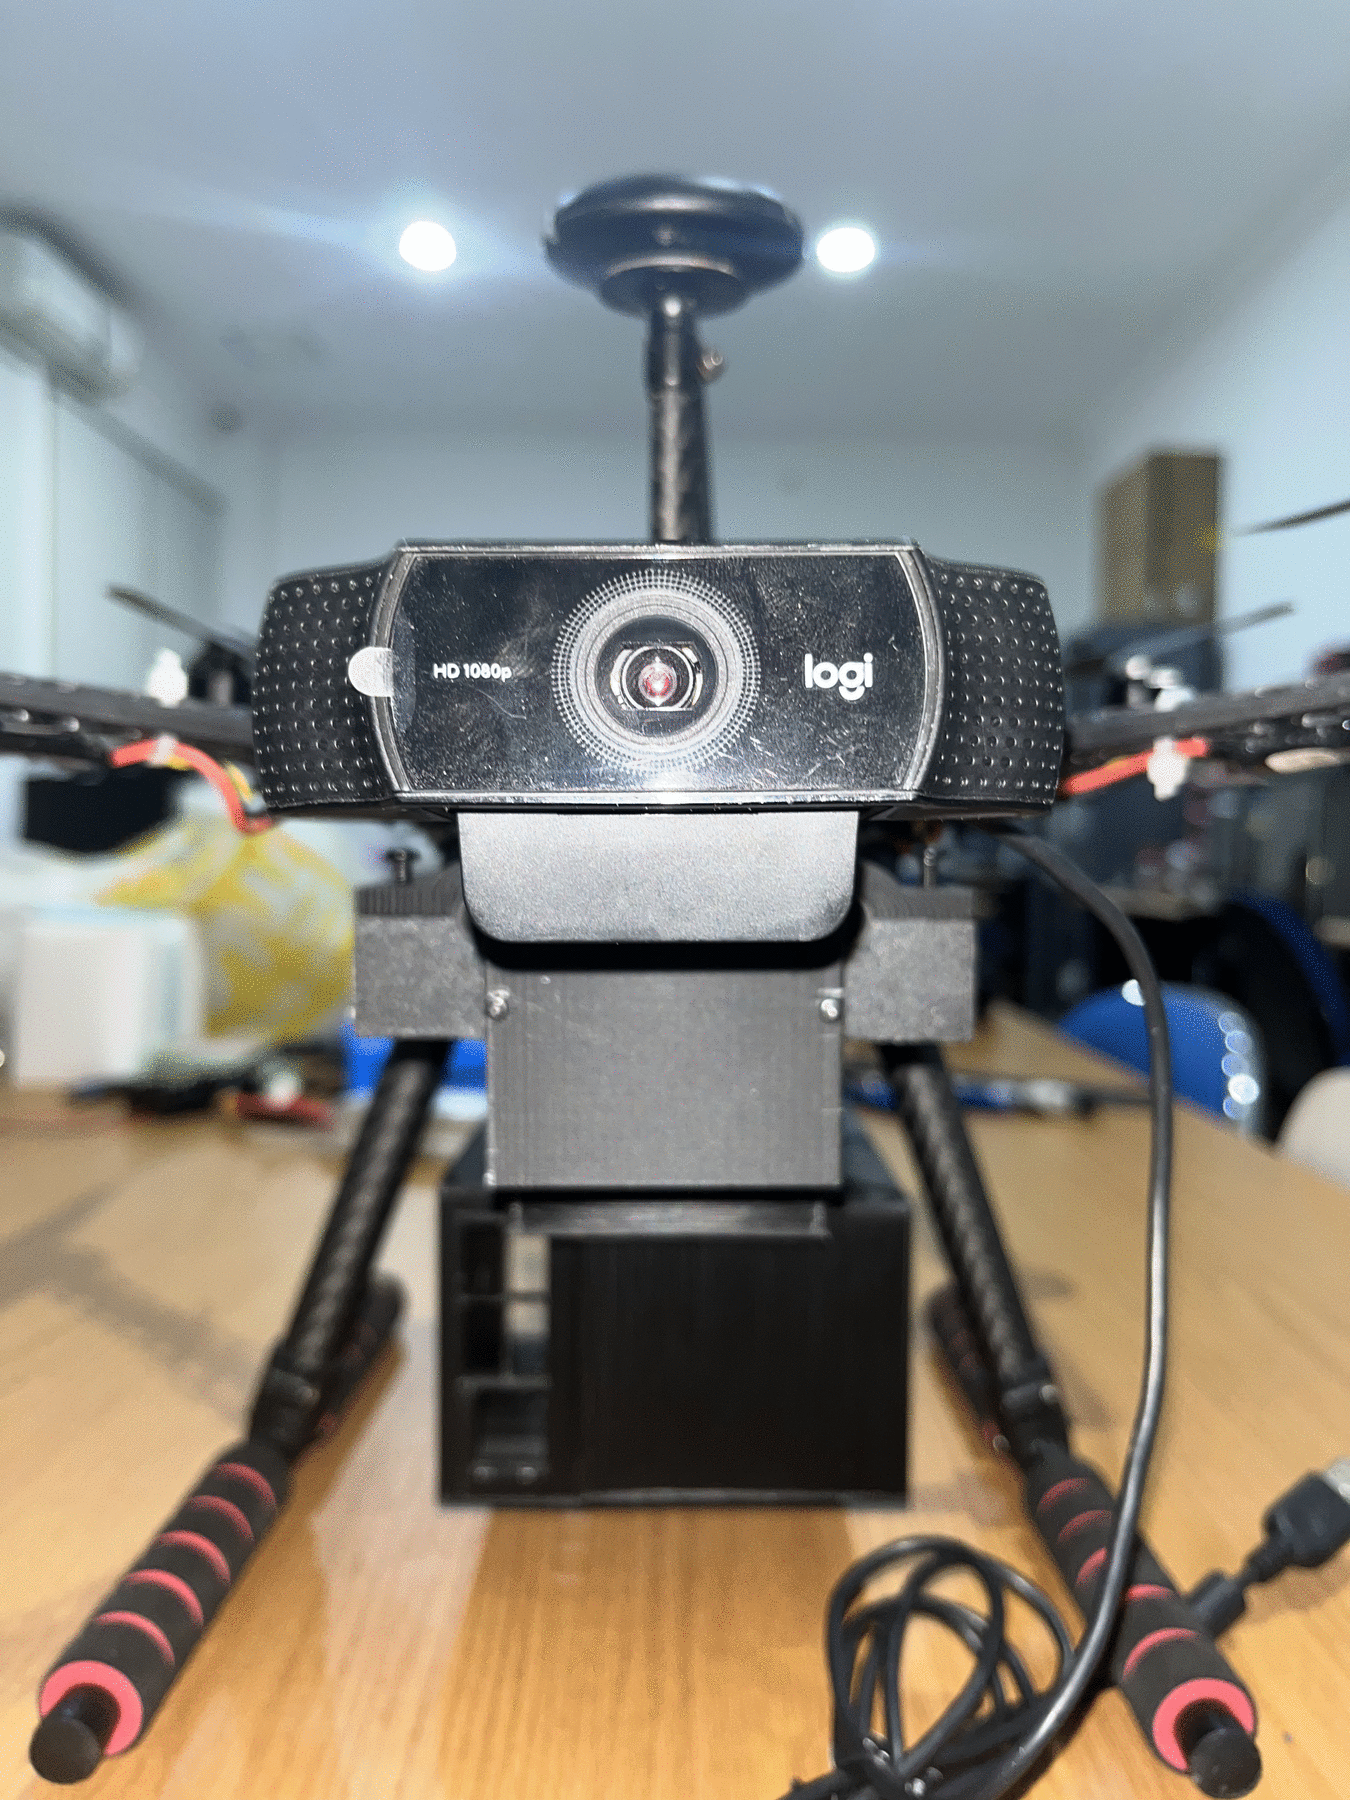
\includegraphics[width=0.7\linewidth]{bab3/full_assembly_real_2}
			\caption{Hasil Realisasi Perakitan Keseluruhan Sistem Tampak Perspektif 2}
			\label{fig:perakitan-keseluruhan-sistem-real-2}
		\end{subfigure}
		\hfill
		\begin{subfigure}[b]{0.3\textwidth}
			\centering
			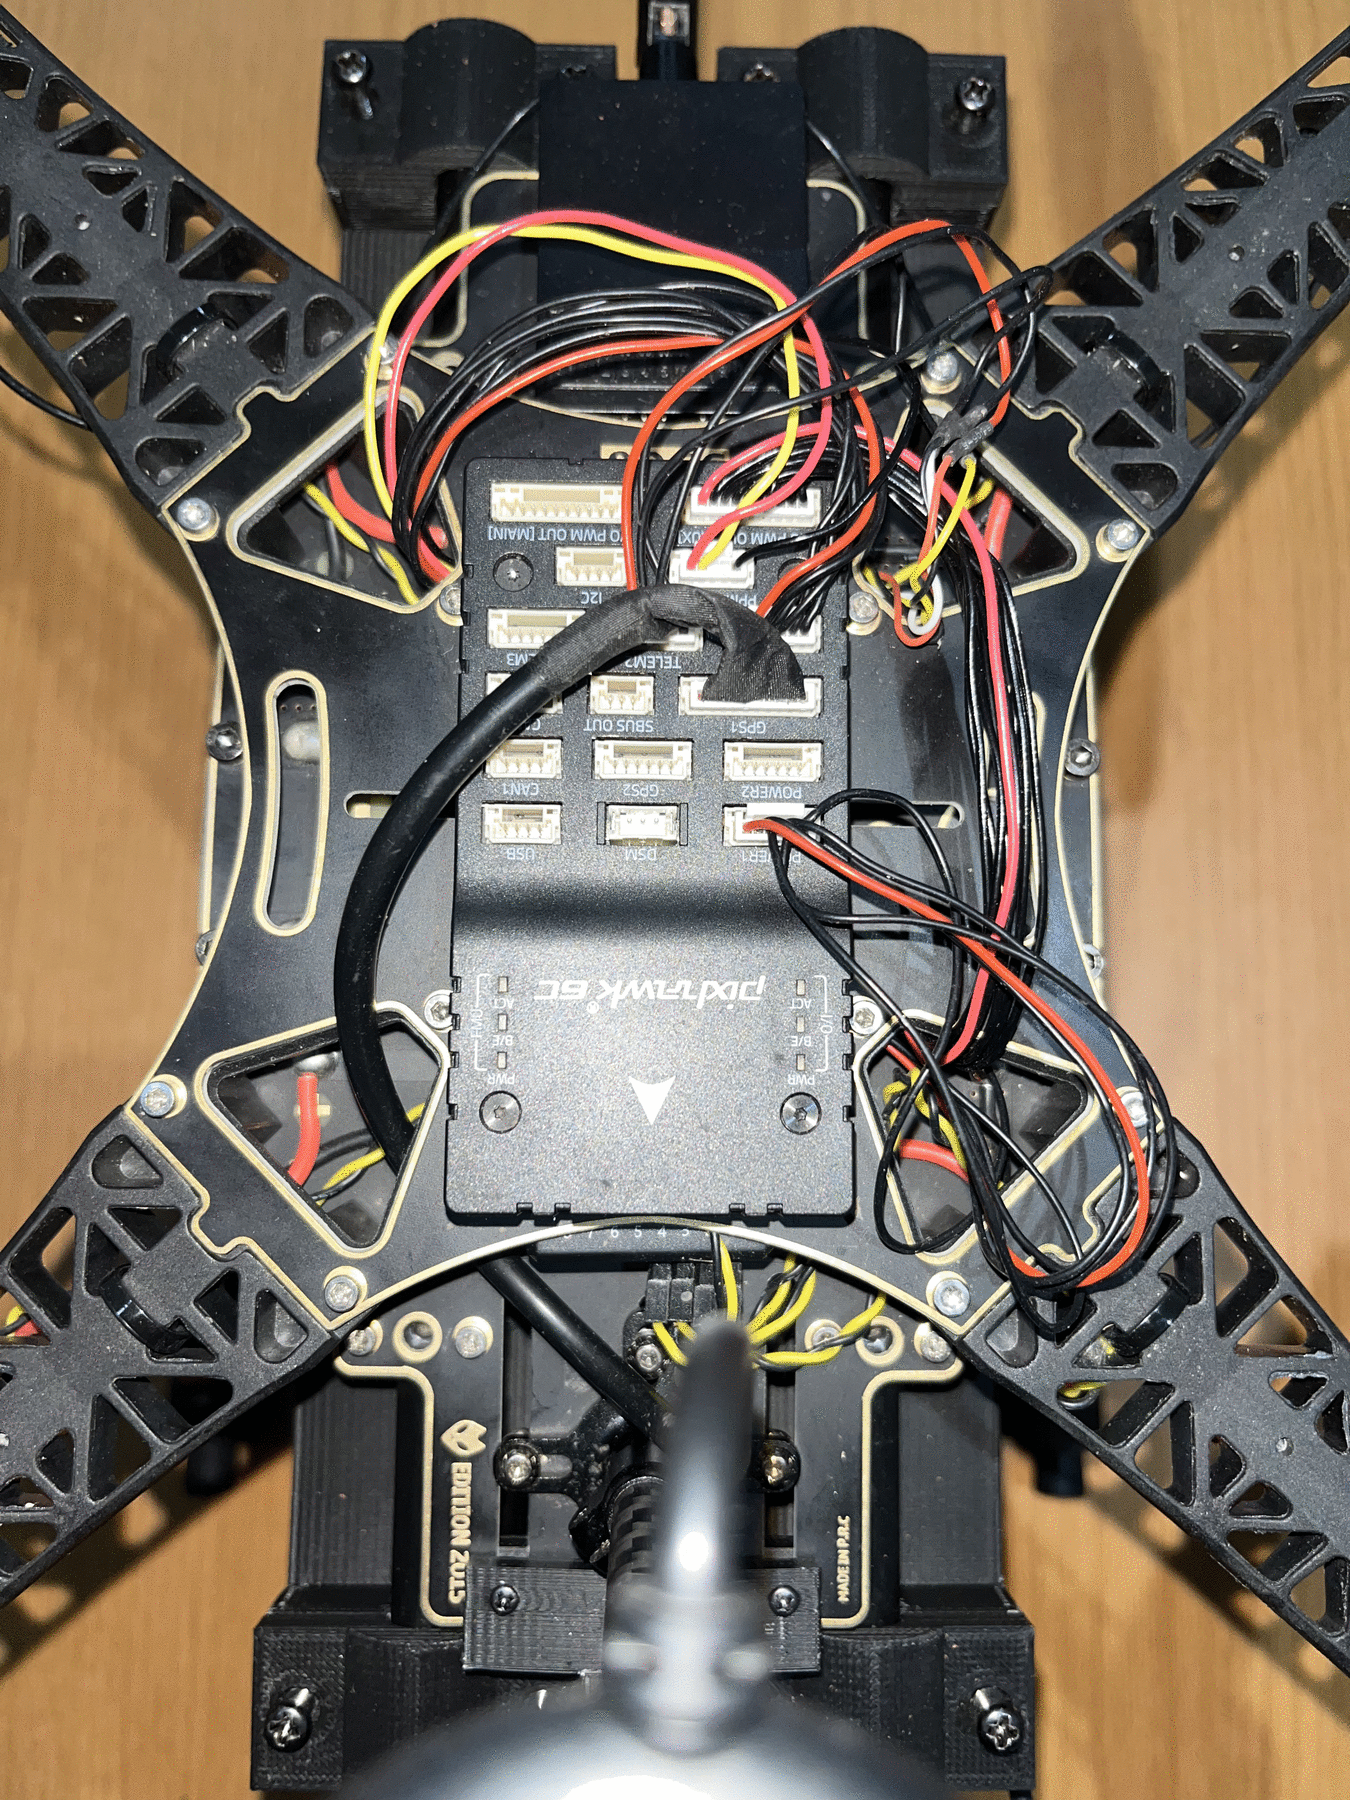
\includegraphics[width=0.7\linewidth]{bab3/full_assembly_real_3}
			\caption{Hasil Realisasi Perakitan Keseluruhan Sistem Tampak Perspektif 3}
			\label{fig:perakitan-keseluruhan-sistem-real-3}
		\end{subfigure}
	\end{figure}
	
	\item Instalasi Modem MiFi 4G/5G: Untuk mendukung komunikasi \textit{dual-mode}, sebuah modem MiFi 4G/5G (\textit{wireless}) ditempatkan di dalam Casing modem. Penempatan ini mempermudah tata letak dan meminimalisir risiko interferensi kabel pada sensor GPS
	\begin{figure}[H]
		\centering
		\begin{subfigure}[b]{0.45\textwidth}
			\centering
			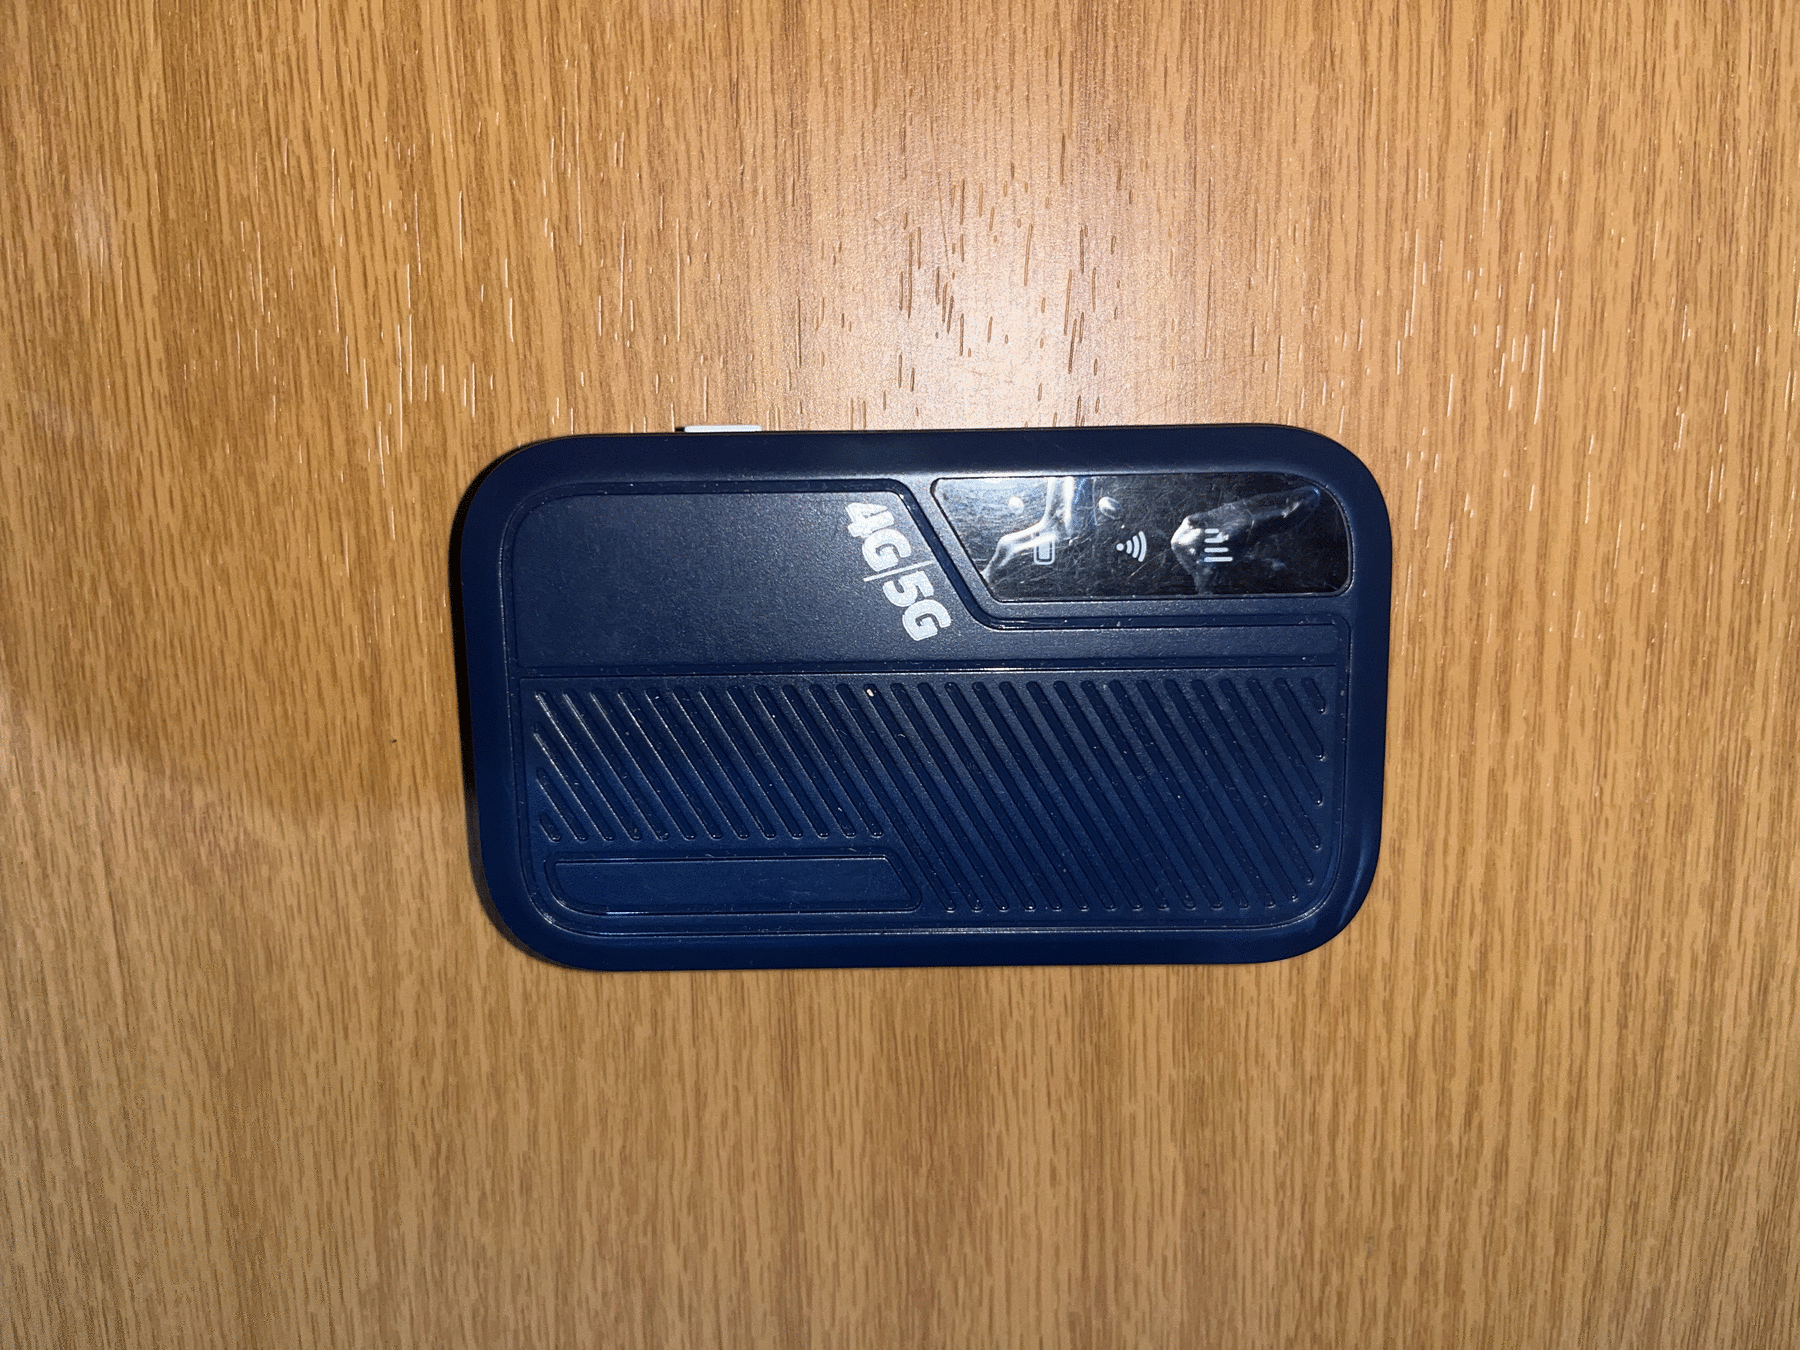
\includegraphics[width=0.9\linewidth]{bab3/modem_mifi_4g}
			\caption{Modem MiFi 4G/5G yang digunakan}
			\label{fig:modem-mifi-4g}
		\end{subfigure}
		\hfill
		\begin{subfigure}[b]{0.45\textwidth}
			\centering
			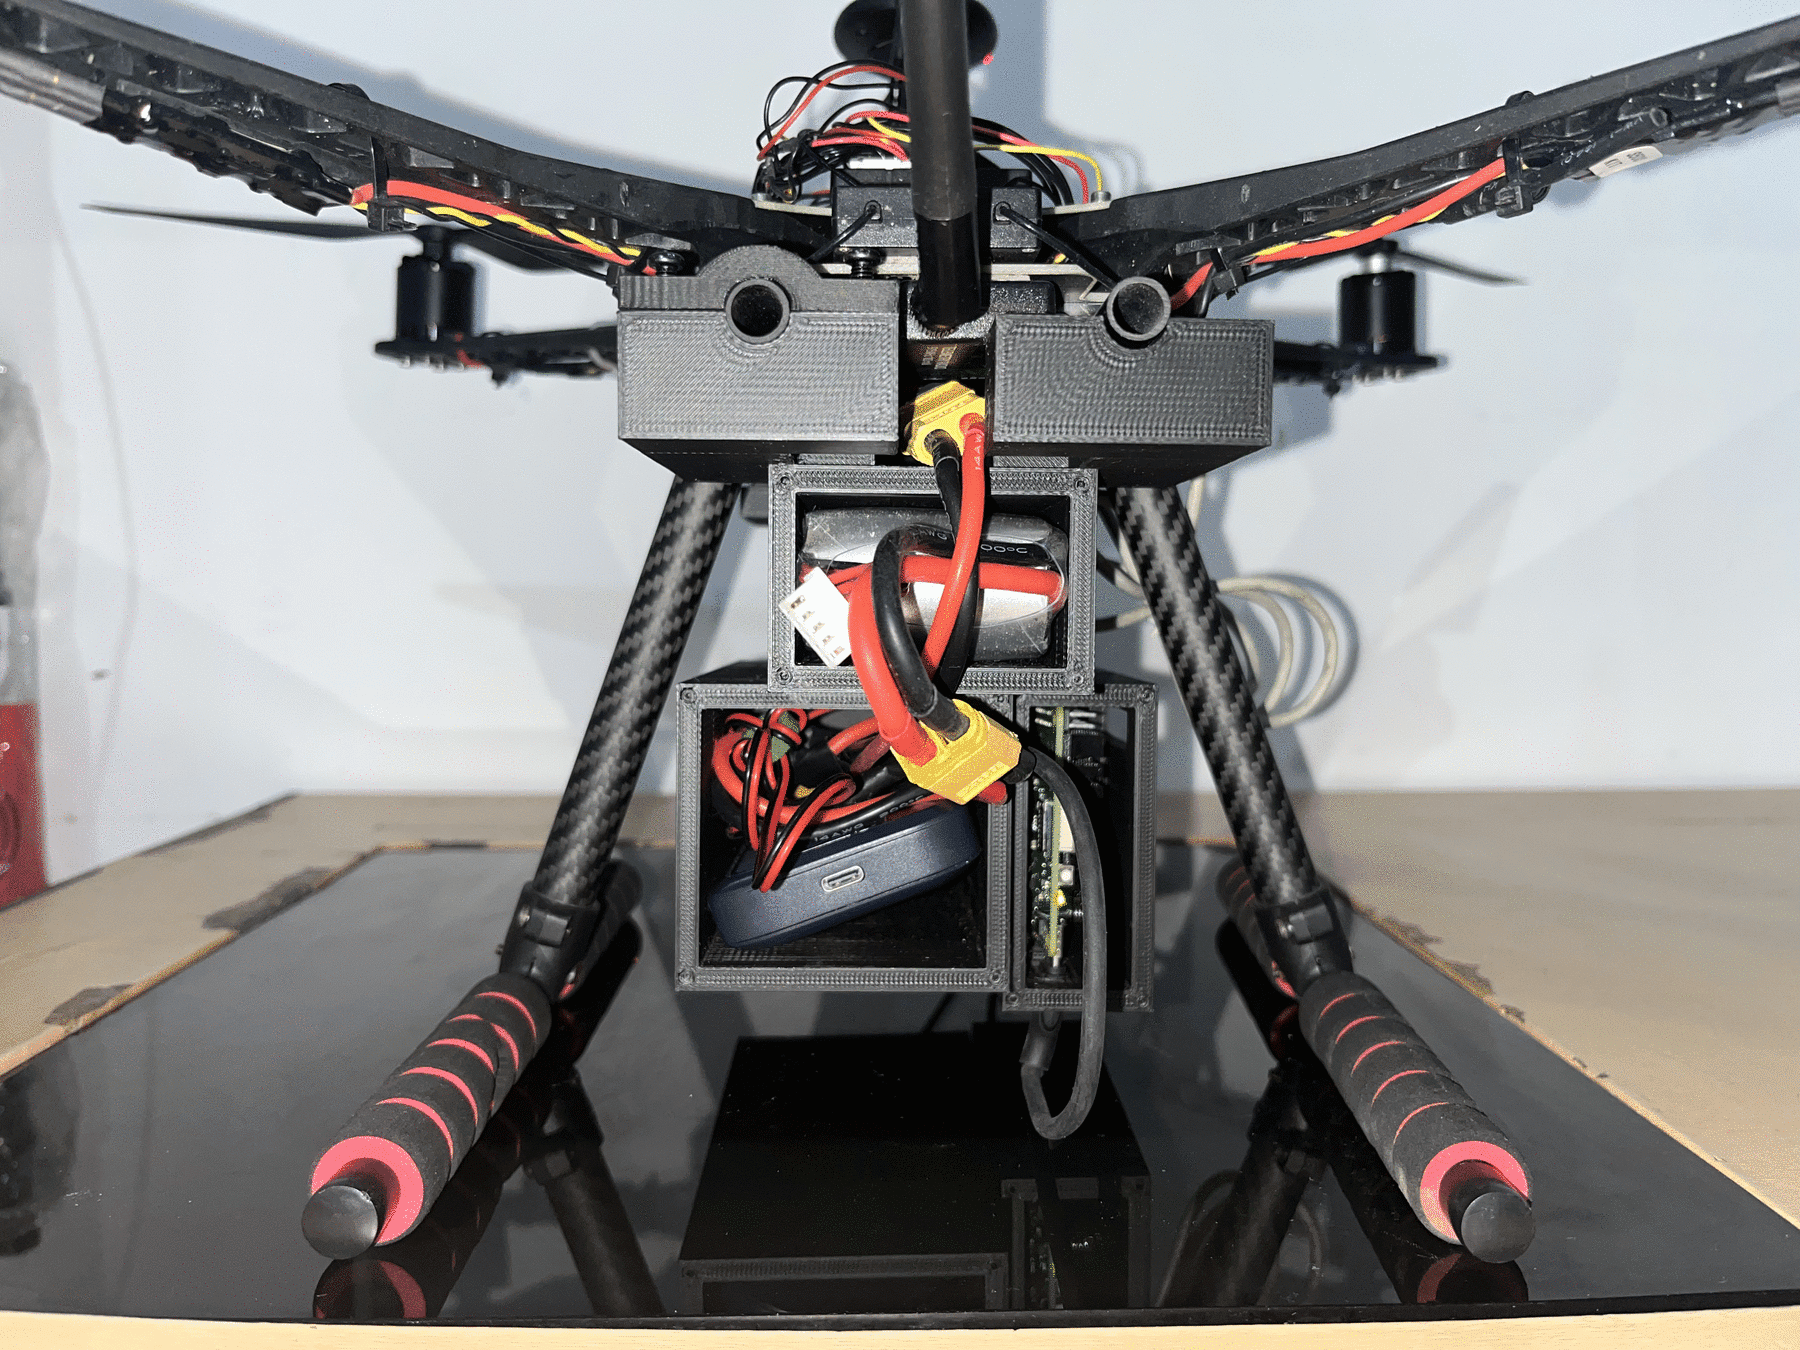
\includegraphics[width=0.9\linewidth]{bab3/modem_mifi_4g_casing}
			\caption{Penempatan Modem MiFi 4G/5G di dalam Casing modem}
			\label{fig:penempatan-modem-mifi-4g}
		\end{subfigure}
	\end{figure}
\end{itemize}

Gambar \ref{fig:modem-mifi-4g} dan Gambar \ref{fig:penempatan-modem-mifi-4g} menunjukkan wujud fisik modem MiFi 4G/5G beserta penempatannya di dalam Casing modem. Berdasarkan implementasi tersebut, integrasi modem ini menyediakan konektivitas internet nirkabel yang stabil untuk pengiriman data telemetri. Dapat diamati bahwa rancangan penempatan modem ini memanfaatkan ruang kosong secara efisien tanpa mengganggu penempatan sensor lainnya. Dengan demikian, seluruh perakitan perangkat keras tambahan telah diselesaikan secara terintegrasi dan siap mendukung fungsionalitas sistem otonom drone.

\subsection{Implementasi Backend System}
Implementasi \textit{backend system} direalisasikan menggunakan bahasa pemrograman Python dengan kerangka kerja Flask. Sistem ini mengadopsi arsitektur \textit{split-brain} dan didistribusikan ke dalam beberapa modul spesifik (telemetri, visi komputer, dan navigasi) yang dikerjakan secara konkuren.

Untuk memberikan gambaran menyeluruh terhadap ruang lingkup pengembangan, perangkat lunak disusun dalam struktur direktori fungsional sebagai berikut:

Arsitektur perangkat lunak pada sistem otonom ini disusun secara modular guna meningkatkan tingkat pemeliharaan (\textit{maintainability}) serta keterkembangan (\textit{scalability}) sistem secara berkelanjutan. Melalui pendekatan modularitas ini, pemisahan tanggung jawab antar-modul (\textit{separation of concerns}) dapat terjaga dengan baik sekaligus memberikan kemudahan bagi pengembangan fitur tambahan di masa depan. Struktur pengorganisasian kode program yang modular tersebut direpresentasikan melalui pembagian direktori kerja yang sistematis.

\begin{lstlisting}[language=bash, caption={Struktur direktori fungsional perangkat lunak sistem drone otonom}]
	/otonom
	|-- /client               # Antarmuka Pengguna (Frontend React 19)
	|   `-- /src
	|       |-- /components   # Representasi visual (Dasbor telemetri)
	|       `-- /services     # Layanan klien untuk koneksi REST API
	|-- /server_flask         # Sistem Backend & Pemrosesan Inti (Flask)
	|   |-- app.py            # Titik masuk & orkestrasi threading
	|   |-- /core             # Mesin keputusan & telemetri
	|   |-- /pipeline         # Subsistem akuisisi video & AI (YOLO)
	|   |-- /web              # Titik akhir komunikasi HTTP server
	|   |-- /photos           # Penyimpanan persisten dokumentasi visual (foto korban)
	|-- start_all.fish        # Skrip otomatisasi inisialisasi program
	`-- yolov8n320.onnx       # Model bobot kecerdasan buatan
\end{lstlisting}

Dengan pembagian fungsional tersebut, implementasi masing-masing layanan diuraikan pada bagian berikut.

\subsubsection{Implementasi Orkestrasi Threading Utama}
Modul utama (\textit{entry point}) berfungsi sebagai pusat pengatur jalannya program. Tujuannya adalah agar proses komputasi berat, seperti deteksi AI dan server web, tidak mengganggu kelancaran pengiriman perintah gerak ke drone. Pada Listing \ref{lst:app_thread}, program dijalankan secara berurutan. Pertama, sistem menyalakan kamera dan AI pendeteksi objek (YOLOv8n) di dalam blok pelindung \texttt{try-except}. Tujuannya agar jika kamera gagal menyala, program langsung berhenti dengan aman. Kedua, sistem menyiapkan jalur komunikasi (API) untuk dasbor pemantauan. Ketiga, program komunikasi ke \textit{flight controller} (MAVSDK) dijalankan di latar belakang (\textit{background thread}) agar tidak menahan proses lain. Terakhir, server web SocketIO dinyalakan untuk memancarkan data ke layar operator secara terus-menerus.

\begin{lstlisting}[language=Python, caption={Inisialisasi arsitektur \textit{multi-threading} pada modul utama}, label={lst:app_thread}]
	try:
	start_pipeline()
	except Exception as e:
	logger.critical(f"FATAL: Pipeline failed to start: {e}")
	sys.exit(1)
	
	register_monitoring_routes(app, get_listener=lambda: mavsdk_listener, ...)
	
	mav_thread = threading.Thread(target=run_async_main, daemon=True, name="MAVSDK-Thread")
	mav_thread.start()
	
	socketio.run(app, host="0.0.0.0", port=3000, debug=False, use_reloader=False)
\end{lstlisting}

\subsubsection{Implementasi Telemetri dan Mekanisme Keepalive}
Modul telemetri bertugas membaca data penerbangan seperti GPS, baterai, dan mode terbang secara rutin menggunakan pustaka \textit{MAVSDK-Python}. Bagian paling krusial di sini adalah mekanisme \textit{keepalive} (Listing \ref{lst:keepalive}). Aturan keselamatan dasar drone (Firmware PX4) mensyaratkan bahwa mode otonom (\textit{OFFBOARD}) baru bisa aktif jika \textit{companion computer} (Raspberry Pi 5) sudah terbukti aktif mengirimkan perintah gerak. Oleh karena itu, selama drone belum masuk mode otonom, sistem akan terus-menerus mengirimkan perintah gerak palsu bernilai nol (\texttt{set\_velocity\_ned}). Proses "detak jantung" ini dikirim sangat cepat (setiap 0,05 detik) agar kapan pun operator menekan tombol otonom, drone sudah dalam kondisi siap dan langsung merespons tanpa ditolak oleh sistem keamanan.

\begin{lstlisting}[language=Python, caption={Rutin \textit{keepalive} untuk menjamin transisi mode penerbangan otonom}, label={lst:keepalive}]
	async def _offboard_keepalive(self):
	logger.info("Offboard keepalive stream dimulai")
	while self._running:
	try:
	if not self.state.get("autonomy_running", False):
	await self.drone.offboard.set_velocity_ned(
	VelocityNedYaw(0.0, 0.0, 0.0, 0.0)
	)
	if not hasattr(self, '_last_keepalive_log') or (_time.time() - self._last_keepalive_log) > 1.0:
	logger.info("KEEPALIVE -> VelocityNedYaw(0.0, 0.0, 0.0, 0.0) -> Pixhawk (stream aktif)")
	self._last_keepalive_log = _time.time()
	await asyncio.sleep(0.05)
	except asyncio.CancelledError:
	break
\end{lstlisting}

\subsubsection{Implementasi Pipeline Video Bebas Blokir}
Pengambilan gambar dari kamera menggunakan GStreamer diatur agar terpisah dari proses deteksi AI. Ketika gambar diterima, sistem akan langsung mengubah format gambarnya menjadi susunan matriks agar bisa dibaca oleh algoritma komputer. Proses suplai gambar ini menggunakan metode antrean bocor atau \textit{leaky queue} (Listing \ref{lst:leaky}). Artinya, jika proses deteksi AI sedang melambat dan antrean gambar sudah terlanjur penuh (\texttt{Full}), sistem kamera tidak akan menunggu (\textit{non-blocking}). Sistem akan otomatis membuang gambar yang paling lama di dalam antrean (\texttt{get\_nowait()}) dan segera menggantinya dengan gambar hasil jepretan terbaru (\texttt{put\_nowait()}). Cara ini memastikan AI selalu menganalisis kondisi lapangan terkini tanpa membuat sistem kamera macet atau mengalami \textit{lag}.

\begin{lstlisting}[language=Python, caption={Penerapan mekanisme \textit{leaky queue} pada penerima aliran video}, label={lst:leaky}]
	frame = np.frombuffer(map_info.data, dtype=np.uint8).reshape((h, w, 3)).copy()
	
	try:
	self.frame_queue.put_nowait(frame)
	except Full:
	try:
	self.frame_queue.get_nowait() 
	self.frame_queue.put_nowait(frame)
	except:
	pass
\end{lstlisting}

\subsubsection{Implementasi Inferensi Visual YOLOv8}
Proses deteksi target AI dijalankan secara mandiri, terpisah dari proses tangkapan kamera. AI ini dikunci agar hanya fokus mencari target "manusia" (kelas 0) pada gambar (Listing \ref{lst:yolocore}). Saat target ditemukan, algoritma mengambil koordinat kotak pembatas objek (\textit{bounding box}) yang bentuk angkanya sudah dinormalisasi menjadi skala 0 hingga 1 (\texttt{box.xyxyn}). Dari angka tersebut, sistem menghitung titik tengah objek (\textit{center x} dan \textit{center y}) serta menghitung seberapa besar objek menutupi layar (\textit{area}). Data matematika inilah yang nantinya diserahkan kepada logika navigasi drone untuk memutuskan ke arah mana drone harus bergerak.

\begin{lstlisting}[language=Python, caption={Ekstraksi parameter sasaran spasial pasca-inferensi Model YOLOv8}, label={lst:yolocore}]
	results = self._pt_model(
	img, conf=self.conf_threshold, iou=self.iou_threshold, classes=[0], verbose=False
	)
	detections = []
	for r in results:
	for box in r.boxes:
	x1, y1, x2, y2 = box.xyxyn[0].tolist()
	cx = (x1 + x2) / 2
	cy = (y1 + y2) / 2
	area = (x2 - x1) * (y2 - y1)
	cls_name = r.names[int(box.cls)]
	
	detections.append(Detection(
	class_name=cls_name, confidence=float(box.conf),
	bbox=[x1, y1, x2, y2], cx=cx, cy=cy, area=area
	))
\end{lstlisting}

\subsubsection{Implementasi Kalkulasi Kendali Proporsional}
Bagian ini bertugas menerjemahkan posisi objek di dalam layar kamera menjadi perintah fisik terbang (Listing \ref{lst:tracking}). Agar pergerakan drone tidak tersendat atau bergetar akibat pergeseran kamera (\textit{jitter}), koordinat titik tengah target dihaluskan menggunakan algoritma \textit{Exponential Moving Average} (EMA). Setelah posisinya dikunci stabil, sistem akan menghitung seberapa jauh target melenceng dari titik tengah layar. Jika target terlalu ke kiri atau ke kanan (\texttt{cx\_error}), drone akan diperintahkan untuk berputar (\textit{yaw}). Jika target berada terlalu atas atau bawah di layar (\texttt{cy\_error}), drone akan bergerak maju (\textit{forward}) untuk menghampiri target secara proporsional sesuai batasan kecepatan maksimal (\texttt{MAX\_VEL}).

\begin{lstlisting}[language=Python, caption={Sistem komputasi navigasi pelacakan otomatis}, label={lst:tracking}]
	def _compute_tracking_command(self, detections, current_yaw, current_alt, vz_alt):
	target = self._select_person_target(detections, ...)
	if target is None:
	return 0.0, 0.0, vz_alt, current_yaw
	
	self._smooth_cx = self._alpha * target["cx_norm"] + (1 - self._alpha) * self._smooth_cx
	self._smooth_cy = self._alpha * target["cy_norm"] + (1 - self._alpha) * self._smooth_cy
	
	cx_error = self._smooth_cx - 0.5
	yaw_cmd = current_yaw + self.KP_YAW * cx_error
	
	cy_error = self._smooth_cy - 0.5
	vn = max(-self.MAX_VEL, min(self.MAX_VEL, self.KP_FORWARD * cy_error))
	
	return vn, 0.0, vz_alt, yaw_cmd
\end{lstlisting}

\subsubsection{Implementasi Diagram Keadaan Navigasi Pencarian}
Skenario misi pencarian (\textit{Scout Mission}) mengatur tahapan gerak drone menggunakan \textit{state machine} yang diintegrasikan dengan arsitektur keselamatan tiga lapis (\textit{Three-Layer Safety System}). Arsitektur keselamatan ini dirancang secara khusus untuk memitigasi risiko kegagalan fatal akibat penyimpangan sensor barometer (\textit{barometric altitude drift}) pada area penerbangan rendah di mana pembacaan ketinggian relatif (\textit{relative altitude}) Pixhawk sering kali melayang jauh lebih tinggi dari kondisi \textit{Above Ground Level} (AGL) sebenarnya (misalnya, pembacaan log menunjukkan ketinggian 1,6 meter sementara kondisi riil wahana hanya berada di bawah 60 cm). Tiga lapis sistem pengamanan keselamatan ini meliputi:

\begin{enumerate}
	\item \textit{Altitude Floor} (Batas Bawah Ketinggian): Pada saat inisialisasi awal maupun selama penerbangan otonom berlangsung, ketinggian target \texttt{\_target\_altitude\_scout} dikunci ke batas bawah keselamatan (\texttt{MIN\_SAFE\_ALTITUDE\_M} sebesar 1,2 meter) untuk mencegah drift barometer memaksa drone terbang terlalu rendah hingga membentur rintangan di permukaan tanah.
	\item \textit{Runtime Altitude Floor Clamp}: Pada setiap iterasi loop kontrol utama (20 Hz), target altitude drone diverifikasi secara dinamis. Apabila nilai target terdeteksi berada di bawah ambang batas aman 1,2 meter, sistem secara aktif menolak dan memaksa nilai tersebut kembali ke batas keselamatan minimum agar perintah kecepatan vertikal (\texttt{vz}) mendorong drone naik kembali ke ketinggian aman.
	\item \textit{Pre-RTL Safety Climb} (Fase Pendakian Sebelum RTL): Ketika tingkat baterai drone kritis di bawah ambang batas ($< 15\%$) atau terjadi perintah darurat (\textit{emergency stop}), drone tidak diizinkan langsung beralih ke mode RTL bawaan autopilot PX4 yang akan memulangkan drone secara horizontal dengan kecepatan tinggi pada ketinggian rendah. Sebagai gantinya, sistem otonom membatalkan seluruh misi dan memasuki fase pendakian keselamatan secara paksa dengan kecepatan vertikal konstan $vz = -0,8$ m/s (ke atas dalam kerangka acuan NED Pixhawk, menghasilkan pertambahan ketinggian sekitar 2,4 meter) selama durasi \texttt{SCOUT\_PRE\_RTL\_CLIMB\_S} (3,0 detik). Setelah mencapai ketinggian aman, gerak horizontal dihentikan sementara (\textit{hold}) sebelum kendali diserahterimakan sepenuhnya ke perintah \textit{Return to Launch} (RTL) PX4.
\end{enumerate}

Mengacu pada Listing \ref{lst:scoutstate}, integrasi \textit{state machine} otonom beserta tiga lapis sistem keselamatan tersebut dijalankan di dalam loop kontrol berfrekuensi 20 Hz.

\begin{lstlisting}[language=Python, caption={Perpindahan \textit{state machine} dengan tiga lapis sistem keselamatan}, label={lst:scoutstate}]
	# 1. Safety Check Baterai & Pre-RTL Climb Phase
	battery = self.state_dict.get("battery_pct", 100)
	if battery < self.BATTERY_RTL_THRESHOLD and not self._battery_rtl_triggered:
		self._battery_rtl_triggered = True
		self._scout_mode = False
		self._scout_state = ScoutState.IDLE
		
		# Prosedur pendakian paksa (pre-RTL safety climb) untuk memitigasi baro-drift
		cur_yaw = self.state_dict.get("attitude", {}).get("yaw", 0.0)
		climb_end = asyncio.get_event_loop().time() + self.SCOUT_PRE_RTL_CLIMB_S
		while asyncio.get_event_loop().time() < climb_end:
			await self.drone.offboard.set_velocity_ned(
				VelocityNedYaw(0.0, 0.0, self.SCOUT_PRE_RTL_VZ, cur_yaw)
			)
			await asyncio.sleep(SCOUT_LOOP_PERIOD)
			
		# Hentikan gerakan sebelum serah terima kontrol ke PX4 RTL
		await self.drone.offboard.set_velocity_ned(VelocityNedYaw(0.0, 0.0, 0.0, cur_yaw))
		await self.drone.action.return_to_launch()
		break

	# 2. Runtime Altitude Floor Clamping
	alt = float(self.state_dict.get("position", {}).get("alt", 0.0))
	target_alt = self._target_altitude_scout if self._target_altitude_scout is not None else alt
	if target_alt < self.MIN_SAFE_ALTITUDE_M:
		target_alt = self.MIN_SAFE_ALTITUDE_M
		self._target_altitude_scout = target_alt

	# Hitung vz otonom dengan redaman saat di area stabil
	vz = max(-self.SCOUT_MAX_VZ, min(self.SCOUT_MAX_VZ, -self.SCOUT_KP_ALT * (target_alt - alt)))
	
	# 3. Eksekusi State Machine Scout
	if self._scout_state == ScoutState.SCAN: 
		await self._scout_state_scan(vz, loop_count)
	elif self._scout_state == ScoutState.APPROACH: 
		await self._scout_state_approach(vz, loop_count)
	elif self._scout_state == ScoutState.DOCUMENT: 
		await self._scout_state_document(vz)
	elif self._scout_state == ScoutState.DISPLACING:
		await self._scout_state_displacing(vz)
\end{lstlisting}

\subsection{Implementasi Frontend Monitoring}
Aplikasi antarmuka pemantauan (\textit{dashboard}) di layar operator dibuat menggunakan pustaka modern React 19 dan Vite. Desain perangkat lunak ini dirancang seringkas mungkin agar dapat menampilkan data langsung secara cepat (\textit{real-time}) tanpa terjadi penundaan parah di pihak operator.

\subsubsection{Implementasi Komunikasi Asinkron Klien}
Komunikasi dua arah antara drone dan layar operator diatur menggunakan teknologi \textit{WebSocket} (Listing \ref{lst:reactsocket}). Jalur komunikasi ini dirancang agar kuat menghadapi kondisi sinyal di lapangan terbuka yang tidak menentu. Apabila koneksi terputus, dasbor secara otomatis akan mencoba menyambung ulang (\texttt{reconnection}) setiap satu detik hingga maksimal 10 kali percobaan. Selama tersambung, antarmuka ini secara konstan akan menangkap data status penerbangan (baterai, tinggi, mode) melalui saluran `drone:status` dan menangkap titik koordinat objek dari AI melalui saluran `yolo:detections` untuk langsung disajikan ke hadapan operator secara interaktif.

\begin{lstlisting}[language=Java, caption={Modul \textit{service} komunikasi \textit{socket} untuk penerimaan siaran telemetri}, label={lst:reactsocket}]
	connect() {
		this.socket = io(apiService.getSocketURL(), {
			transports: ['websocket', 'polling'],
			reconnection: true,
			reconnectionDelay: 1000,
			reconnectionAttempts: 10
		});
		
		this.socket.on('drone:status', (data) => {
			this.emit('drone:status', data);
		});
		
		this.socket.on('yolo:detections', (data) => {
			this.emit('yolo:detections', data);
		});
		
		return this.socket;
	}
\end{lstlisting}
Seluruh data yang diterima melalui saluran soket (khususnya \texttt{drone:status}) langsung diubah menjadi tampilan visual pada layar dasbor operator. Panel status bertugas menampilkan informasi penting penerbangan secara praktis, seperti ketinggian drone, sisa baterai, dan status sinyal satelit GPS. Sementara itu, pada panel pemutar video, sistem bertugas menampilkan siaran langsung dari kamera drone sekaligus menggambar kotak pembidik sasaran (\textit{Virtual Overlay HUD}) yang ditumpuk tepat di atas video tersebut secara interaktif.
\subsection{Integrasi Sistem Keseluruhan}

Tahap integrasi akhir memastikan seluruh subsistem—mulai dari struktur mekanik, kelistrikan, hingga arsitektur perangkat lunak—bekerja secara sinkron dan stabil melalui alur kerja komprehensif berikut:

\begin{enumerate}
	\item Integrasi Mekanik dan Perangkat Keras \\
	Rangkaian perangkat keras tambahan, termasuk \textit{companion computer} (\textit{Raspberry Pi 5}) dan sensor visual (\textit{kamera Logitech C922}), diintegrasikan pada rangka \textit{Holybro S500} menggunakan komponen cetak 3D. Penempatan seluruh modul dirancang secara simetris di bagian tengah bawah drone untuk menjaga \textit{Center of Gravity} (CG) agar keseimbangan aerodinamis tetap optimal selama penerbangan otonom.
	
	\item Kestabilan Suplai Daya \\
	Kebutuhan daya komputasi yang tinggi diatasi melalui integrasi modul regulator \textit{UBEC 5A} yang terhubung langsung dengan baterai \textit{LiPo} utama drone. Skema kelistrikan ini memastikan suplai tegangan 5V yang stabil dan terisolasi ke \textit{Raspberry Pi 5}, sehingga mencegah terjadinya \textit{voltage sag} atau mati mendadak saat motor penggerak menarik arus puncak.
	
	\item Akuisisi dan Pemrosesan Visual \\
	Pada sisi perangkat lunak, \textit{GStreamer} bertugas menangkap aliran video dari kamera dan mendistribusikannya secara \textit{non-blocking} ke \textit{thread YOLOv8}, di mana proses inferensi deteksi target manusia dilakukan secara \textit{real-time}.
	
	\item Pengambilan Keputusan Otonom \\
	Hasil deteksi visual spasial kemudian dipadukan dengan data telemetri dari \textit{Flight Controller Pixhawk} oleh \textit{thread MAVSDK}. Sistem memproses data tersebut melalui \textit{State Machine} untuk menentukan tindakan navigasi selanjutnya secara dinamis.
	
	\item Eksekusi Navigasi Penerbangan \\
	Keputusan dari \textit{State Machine} diterjemahkan menjadi perintah kecepatan (vektor \texttt{VelocityNedYaw}) dan dikirimkan kembali ke \textit{Pixhawk}. Selama mode penerbangan \textit{OFFBOARD} aktif, \textit{Pixhawk} akan mengeksekusi perintah tersebut menjadi pergerakan motor fisik secara otomatis.
	
	\item Sistem Keselamatan dan Prosedur Pengamanan (\textit{Safety Procedure}) \\
	Integritas misi dilindungi secara berlapis oleh sistem pengawasan (\textit{watchdog}) dan arsitektur keselamatan terpadu. Apabila terdeteksi kondisi kritis baterai rendah di bawah ambang batas ($< 15\%$) atau hilangnya koneksi telemetri, sistem secara asinkron memicu prosedur pendakian darurat (\textit{pre-RTL safety climb}) selama 3,0 detik pada kecepatan $0,8$ m/s ke atas untuk mencapai ketinggian aman sebelum mengaktifkan perintah \textit{Return to Launch} (RTL) otonom bawaan PX4. Mekanisme pendakian darurat ini krusial guna mencegah benturan akibat penyimpangan pembacaan ketinggian barometer (\textit{barometric altitude drift}) pada area penerbangan rendah. Selain itu, operator di darat memegang kendali prioritas tertinggi melalui \textit{Remote Controller} untuk melakukan pengambilalihan manual (\textit{manual override}) kapan saja demi alasan keselamatan penerbangan.
	
	\item Pengawasan Operator (\textit{Monitoring}) \\
	Seluruh data operasional, status terbang, dan tangkapan visual dipancarkan secara kontinu ke \textit{frontend monitoring} melalui koneksi jaringan nirkabel (\textit{Wi-Fi} lokal atau modem \textit{MiFi 4G/5G}), memungkinkan operator melakukan pengawasan misi pencarian secara presisi.
\end{enumerate}

Melalui integrasi menyeluruh ini, sistem tidak hanya mampu menjalankan proses akuisisi citra, deteksi target, dan navigasi otomatis, tetapi juga menjamin keandalan struktural, stabilitas kelistrikan, serta keselamatan operasional selama misi pencarian korban berlangsung. Seluruh konfigurasi mekanik akhir hasil penyempurnaan pada bagian konektor dudukan ini selanjutnya digunakan secara penuh pada seluruh tahapan pengujian sistem otonom yang dijabarkan pada Bab IV.